\documentclass[11pt,a4paper]{report}

% ==================== 导言区 ====================
\usepackage[UTF8]{ctex}              % 中文支持
\usepackage{geometry}                % 页面边距
\usepackage{amsmath,amssymb,amsthm}  % 数学环境
\usepackage{mathtools}               % 数学工具
\usepackage{enumitem}                % 列表定制
\usepackage{xcolor}                  % 颜色
\usepackage{graphicx}                % 图片插入
\usepackage{booktabs}                % 三线表
\usepackage{hyperref}                % 超链接
\usepackage{fancyhdr}                % 页眉页脚
\usepackage{titlesec}                % 标题格式
\usepackage{multicol}                % 多栏排版
\usepackage{tikz}                    % 绘图
\usetikzlibrary{shapes.geometric, arrows.meta, positioning}

% 页面设置
\geometry{left=2.5cm,right=2.5cm,top=2.5cm,bottom=2.5cm}

% 颜色定义
\definecolor{maincolor}{RGB}{0,82,147}
\definecolor{accentcolor}{RGB}{230,126,34}
\definecolor{lightgray}{RGB}{245,245,245}

% 标题格式
\titleformat{\chapter}{\Large\bfseries\color{maincolor}}{\thechapter}{1em}{}
\titleformat{\section}{\large\bfseries\color{maincolor!80}}{\thesection}{1em}{}
\titleformat{\subsection}{\normalsize\bfseries\color{maincolor!60}}{\thesubsection}{1em}{}

% 定理环境
\theoremstyle{definition}
\newtheorem{definition}{定义}[chapter]
\newtheorem{example}{例}[chapter]
\newtheorem{note}{注}[chapter]
\newtheorem{property}{性质}[chapter]
\newtheorem{theorem}{定理}[chapter]
\newtheorem{warning}{注意}[chapter]
\newtheorem{lemma}{引理}[chapter]

% 页眉页脚
\pagestyle{fancy}
\fancyhf{}
\fancyhead[L]{\small 概率论与数理统计 · 笔记}
\fancyhead[R]{\small \thepage}
\renewcommand{\headrulewidth}{0.4pt}

% 超链接设置
\hypersetup{colorlinks=true,linkcolor=maincolor,citecolor=maincolor,urlcolor=maincolor}

% 自定义命令
\newcommand{\E}{\mathbb{E}}
\newcommand{\Var}{\mathrm{Var}}
\newcommand{\Cov}{\mathrm{Cov}}
\newcommand{\diff}{\,\mathrm{d}}
\newcommand{\iid}{\stackrel{\text{i.i.d.}}{\sim}}

\begin{document}

% ==================== 封面 ====================
\begin{titlepage}
\centering
\vspace*{3cm}
{\Huge\bfseries\color{maincolor} 概率论与数理统计}\\[0.8cm]
{\Large\color{gray} 课程笔记}\\[2cm]
{\large 主讲：陈熙霖、常虹 \quad 助教：闵越聪、李彦辰}\\[0.5cm]
{\large 2025年春季学期}\\[3cm]
\begin{tikzpicture}
\node[draw=maincolor, rounded corners=10pt, inner sep=15pt, line width=1.5pt] {
\begin{minipage}{0.6\textwidth}
\centering
\textit{``概率是相对的，部分出于某种无知，部分出于我们的知识所限。''}\\[0.3cm]
\hfill --- 拉普拉斯
\end{minipage}
};
\end{tikzpicture}
\vfill
{\small 整理日期：\today}
\end{titlepage}

\tableofcontents
\newpage

% ==================== 绪论 ====================
\newpage
\chapter*{绪论}

\section{概率论的研究对象}
\begin{itemize}[leftmargin=2em]
    \item \textbf{必然现象}：在一定条件下必然出现的现象。
    \item \textbf{随机现象}：在一定条件下可能出现也可能不出现的现象。
\end{itemize}

\begin{note}
概率论是研究客观世界\textbf{随机现象数量规律}的学科。
\end{note}

\section{发展简史}
\begin{enumerate}[leftmargin=2em]
    \item \textbf{16世纪}：意大利学者开始研究掷骰子（Chevalier de M\'{e}r\'{e}问题）。
    \item \textbf{17世纪}：帕斯卡、费马等解决``赌徒分金''问题，标志概率论诞生。
    \item \textbf{17--18世纪}：伯努利奠定概率论基础；拉普拉斯引入\textbf{分析概率}。
    \item \textbf{20世纪}：柯尔莫哥洛夫建立\textbf{公理化概率理论体系}。
\end{enumerate}

\section{三类概率意义}
\begin{table}[htbp]
\centering
\caption{三类概率的比较}
\begin{tabular}{@{}lll@{}}
\toprule
\textbf{类型} & \textbf{核心思想} & \textbf{典型例子} \\
\midrule
古典概率/先验概率 & 等可能结果，$P = k/n$ & 掷骰子、抛硬币 \\
频率概率/统计概率 & 大量重复观察的频率稳定值 & 统计估计 \\
分析概率 & 以数学分析（测度论）为基础 & 公理化体系 \\
\bottomrule
\end{tabular}
\end{table}

\section{数理统计}
数理统计研究如何有效地\textbf{收集、整理和分析}带有随机性的数据，并对所考察的问题作出推断或预测，为决策提供依据。

\begin{note}
概率是数理统计的\textbf{基础}，数理统计是概率的\textbf{应用}。
\end{note}

\section{概率的应用领域}
\begin{multicols}{2}
\begin{itemize}[leftmargin=1em,itemsep=0pt]
    \item 机器学习、模式识别
    \item 电子系统、航空航天（可靠性）
    \item 制造业（产品抽样）
    \item 保险业（赔付赔率）
    \item 医学（治疗有效性检验）
    \item 人口调查（抽样）
    \item 传染病流行（生灭过程）
\end{itemize}
\end{multicols}

% ==================== 经典问题 ====================
\section{经典概率问题}

\subsection{非传递骰子（Non-transitive Dice）}
类似于``石头剪刀布''的骰子构造：存在一组骰子 $A,B,C,D$，使得
\[
P(A>B) > \frac{1}{2},\quad P(B>C) > \frac{1}{2},\quad P(C>D) > \frac{1}{2},\quad P(D>A) > \frac{1}{2}.
\]
即骰子间形成\textbf{非传递}的循环优势关系。

\begin{figure}[htbp]
    \centering
    
\includegraphics[width=0.5\textwidth]{figures/fig_ntdice.png}
    \caption{非传递骰子示意图（红、黄、蓝、绿四色骰子）}
    \label{fig:ntdice}
\end{figure}

\subsection{Monty Hall 问题}
\textbf{设定}：三扇门后分别是一辆车和两只羊。参赛者选定一扇门后，主持人（知道门后情况）从剩余两扇门中打开一扇有羊的门。

\textbf{问题}：参赛者应坚持原选择还是换门？

\textbf{分析}：设参赛者最初选择门1。
\begin{itemize}[leftmargin=2em]
    \item 若车在门1（概率 $1/3$），换门失败。
    \item 若车在门2或门3（概率 $2/3$），主持人必打开另一扇有羊的门，换门成功。
\end{itemize}
\[
\boxed{P(\text{换门获胜}) = \frac{2}{3},\quad P(\text{坚持获胜}) = \frac{1}{3}}
\]

\subsection{独生子女问题}
\textbf{问题1}：若老大是女儿，允许生第二个孩子，是否会破坏男女比例？

\textbf{答}：不会。每次生育的性别独立，条件概率不改变总体比例。

\textbf{问题2}：一个家庭有两个孩子，已知其中一个是女孩，另一个也是女孩的概率是多少？

\textbf{答}：样本空间为 $\{GG, GB, BG\}$（排除 $BB$），故 $P = \dfrac{1}{3}$。

\subsection{抛硬币决定命运}
连续抛硬币，直到最近三次出现``正反反''（HTT）或``反反正''（TTH）为止。

\textbf{关键}：前两次结果决定命运。若前两次为``反反''，则后者（TTH）必胜；否则前者（HTT）有优势。

\subsection{路边游戏（公平性分析）}
\textbf{游戏1（抛硬币）}：双方各抛一枚硬币。
\begin{itemize}[leftmargin=2em]
    \item 两正：艺人付参与者 3 元
    \item 两反：艺人付参与者 1 元
    \item 一正一反：参与者付艺人 2 元
\end{itemize}

\textbf{游戏2（亮硬币）}：规则同上，但双方主动亮出硬币。

\textbf{分析}：设参与者选择正面概率为 $p$，艺人选择正面概率为 $q$。
\[
\E[\text{收益}] = 3pq + 1(1-p)(1-q) - 2[p(1-q)+(1-p)q].
\]
在亮硬币游戏中，参与者可根据对方策略调整；抛硬币游戏则纯随机。两者公平性不同，\textbf{亮硬币游戏}可通过策略占优。

\subsection{俄罗斯轮盘赌}
左轮手枪有6个弹仓，$k$ 颗连续子弹，双方轮流对自己开枪。

\textbf{核心}：计算先手与后手的生存概率，关键在于子弹的连续分布与位置轮换。

\subsection{统计的障眼法——辛普森悖论}
\textbf{背景}：1986年肾结石手术成功率统计。

\begin{table}[htbp]
\centering
\caption{手术成功率对比}
\begin{tabular}{@{}lcc@{}}
\toprule
& \textbf{手术A} & \textbf{手术B} \\
\midrule
小块结石 & 93\% (81/87) & 87\% (234/270) \\
大块结石 & 73\% (192/263) & 69\% (55/80) \\
\midrule
\textbf{合计} & 78\% (273/350) & 83\% (289/350) \\
\bottomrule
\end{tabular}
\end{table}

\textbf{悖论}：分组比较中手术A更优，但合计时手术B更优。原因在于两组样本量差异大（混杂变量）。

\subsection{计数与空间的骗局}
\textbf{问题}：妈妈随机去两个兄弟家做饭，哪边地铁先到就去哪边。哥哥比弟弟吃到妈妈做的饭次数多很多，为什么？

\textbf{原因}：\textbf{计数空间不均匀}。例如地铁时刻表：
\begin{itemize}[leftmargin=2em]
    \item 去哥哥家：10:00, 10:10, 10:20, \dots（间隔10分钟）
    \item 去弟弟家：10:02, 10:12, 10:22, \dots（间隔10分钟）
\end{itemize}
妈妈在随机时刻到达，更可能赶上先到的哥哥家地铁（因为时间窗口更大）。

\begin{figure}[htbp]
    \centering
    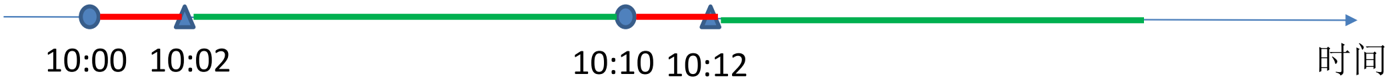
\includegraphics[width=0.8\textwidth]{figures/fig_timeaxis.png}
    \caption{时间轴上的不均匀计数示意图}
    \label{fig:timeaxis}
\end{figure}

% ==================== 课程概览 ====================
\section{课程概览}

\subsection{主要内容}
\begin{itemize}[leftmargin=2em]
    \item \textbf{第一部分：概率论}
    \begin{enumerate}[label=\arabic*.,leftmargin=1em]
        \item 随机事件与概率
        \item 随机变量及其分布
        \item 多维随机变量及其分布
        \item 随机变量的数字特征
        \item 大数定律及中心极限定理
    \end{enumerate}
    \item \textbf{第二部分：数理统计}
    \begin{enumerate}[label=\arabic*.,leftmargin=1em]
        \item 样本及抽样分布
        \item 参数估计
        \item 假设检验
        \item 方差分析
        \item $*$ 随机过程、马尔可夫链、平稳过程
        \item $*$ Bayes统计推断、因果推断
    \end{enumerate}
\end{itemize}

\subsection{教材与参考书}
\begin{enumerate}[leftmargin=2em]
    \item 盛聚、谢式千、潘承毅. \textit{概率论与数理统计}. 高等教育出版社, 2014.
    \item 威廉·费勒. \textit{概率论及其应用}. 人民邮电出版社, 2014.
    \item 拉普拉斯. \textit{关于概率的哲学随笔}（龚光鲁、钱敏平译）. 高等教育出版社.
\end{enumerate}

\subsection{成绩构成}
\begin{itemize}[leftmargin=2em]
    \item 作业：30\%
    \item 期中考试：30\%
    \item 期末考试：40\%
\end{itemize}

% ==================== 第一章 ====================
\newpage
\chapter{随机事件与概率}

\section{随机事件及其概率}

\subsection{随机试验}
满足以下三个条件的试验称为\textbf{随机试验}（记为 $E$）：
\begin{enumerate}[leftmargin=2em]
    \item 可在相同条件下重复进行；
    \item 一次试验前无法确定具体结果；
    \item 能确定所有可能结果。
\end{enumerate}

\subsection{样本空间与样本点}
\begin{definition}[样本空间]
随机试验的所有可能结果组成的集合称为\textbf{样本空间}，记为 $\Omega$（或 $S$）。
\end{definition}

\begin{definition}[样本点与事件]
\begin{itemize}[leftmargin=1em]
    \item \textbf{样本点}：样本空间的单个元素，记为 $e$ 或 $\omega$。
    \item \textbf{随机事件}：样本空间的任意子集，记为 $A,B,C$ 等。
    \item \textbf{基本事件}：由单个样本点组成的集合。
\end{itemize}
\end{definition}

\textbf{两个特殊事件}：
\begin{itemize}[leftmargin=2em]
    \item \textbf{必然事件}：$\Omega$（一定发生）
    \item \textbf{不可能事件}：$\varnothing$（一定不发生）
\end{itemize}

\subsection{事件的关系与运算}
设 $A,B \subseteq \Omega$，则：

\begin{table}[htbp]
\centering
\caption{事件的集合运算}
\begin{tabular}{@{}lll@{}}
\toprule
\textbf{运算} & \textbf{符号} & \textbf{含义} \\
\midrule
包含 & $A \subseteq B$ & $A$发生必导致$B$发生 \\
并（和） & $A \cup B$ & $A$与$B$至少一个发生 \\
交（积） & $A \cap B$（或 $AB$） & $A$与$B$同时发生 \\
差 & $A \setminus B$（或 $A-B$） & $A$发生而$B$不发生 \\
对立（补） & $\bar{A}$（或 $A^c$） & $A$不发生 \\
互斥 & $A \cap B = \varnothing$ & $A$与$B$不能同时发生 \\
\bottomrule
\end{tabular}
\end{table}

\textbf{运算律}：
\begin{align*}
&\text{交换律：} && A \cup B = B \cup A,\quad A \cap B = B \cap A \\
&\text{结合律：} && (A \cup B) \cup C = A \cup (B \cup C) \\
&\text{分配律：} && A \cup (B \cap C) = (A \cup B) \cap (A \cup C) \\
&\text{De Morgan律：} && \overline{A \cup B} = \bar{A} \cap \bar{B},\quad \overline{A \cap B} = \bar{A} \cup \bar{B}
\end{align*}

\begin{example}[掷三枚硬币]
设 $A,B,C$ 分别表示三枚硬币正面朝上。则：
\begin{itemize}[leftmargin=2em]
    \item ``至少一枚正面''：$A \cup B \cup C$
    \item ``恰有一枚正面''：$A\bar{B}\bar{C} \cup \bar{A}B\bar{C} \cup \bar{A}\bar{B}C$
    \item ``三次同一面''：$AB C \cup \bar{A}\bar{B}\bar{C}$
\end{itemize}
\end{example}

\section{频率与概率}

\subsection{频率的定义}
在 $n$ 次重复试验中，事件 $A$ 发生 $n_A$ 次，则
\[
f_n(A) = \frac{n_A}{n}
\]
称为 $A$ 发生的\textbf{频率}。

\textbf{基本性质}：
\begin{enumerate}[leftmargin=2em]
    \item $0 \leq f_n(A) \leq 1$；
    \item $f_n(\Omega) = 1$；
    \item 若 $A_1, A_2, \dots, A_k$ 两两互斥，则
    \[
    f_n\left(\bigcup_{i=1}^k A_i\right) = \sum_{i=1}^k f_n(A_i).
    \]
\end{enumerate}

\subsection{蒲丰投针（Buffon's Needle）}
\textbf{问题}：平面上画有间距为 $d$ 的平行线，随机投掷长度为 $l$ 的针，求针与线相交的概率。

\textbf{思路}：
\begin{enumerate}[leftmargin=2em]
    \item 设针中点到最近平行线距离为 $y \in [0, d/2]$，针与线夹角为 $\theta \in [0, \pi]$。
    \item 相交条件：$y \leq \dfrac{l}{2}\sin\theta$。
    \item 由几何概型：
    \[
    P = \frac{\int_0^\pi \frac{l}{2}\sin\theta \,\diff\theta}{\frac{d}{2} \cdot \pi} = \frac{2l}{\pi d}.
    \]
\end{enumerate}

\textbf{应用}：通过大量投针实验，统计交点数 $m$，可估算圆周率：
\[
\boxed{\pi \approx \frac{2l \cdot n}{m \cdot d}}
\]
其中 $n$ 为投针次数。

\begin{figure}[htbp]
    \centering
    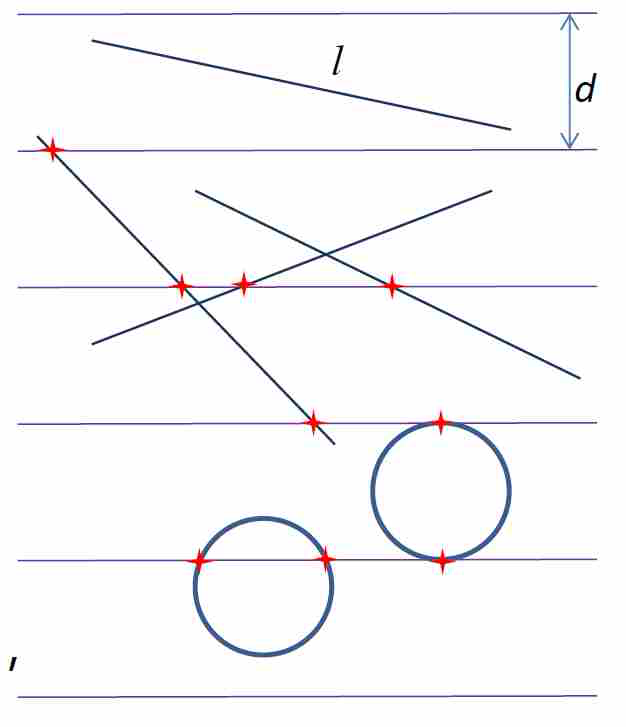
\includegraphics[width=0.7\textwidth]{figures/fig_buffon.png}
    \caption{蒲丰投针示意图（针与平行线相交）}
    \label{fig:buffon}
\end{figure}

\vfill
\begin{center}
\rule{0.6\textwidth}{0.4pt}\\[0.5em]
\textit{``生活中最重要的问题，其中绝大多数在实质上只是概率的问题。''}\\
--- 拉普拉斯
\end{center}

% ==================== §2 频率与概率（续）====================
\section{概率的公理化定义}

\begin{definition}[Kolmogorov 公理]
设 $E$ 是随机试验，$\Omega$ 是其样本空间。对于 $E$ 的每一个事件 $A$，赋予一个实数 $P(A)$。若集合函数 $P(\cdot)$ 满足以下三条，则称 $P(A)$ 为事件 $A$ 的\textbf{概率}：
\begin{enumerate}[label=(\arabic*),leftmargin=2em]
    \item \textbf{非负性}：对任意事件 $A$，有 $P(A) \geq 0$；
    \item \textbf{规范性}：$P(\Omega) = 1$；
    \item \textbf{可列可加性}：若 $A_1, A_2, \dots$ 是两两互不相容的事件（即 $A_i \cap A_j = \varnothing,\; i \neq j$），则
    \[
    P\left(\bigcup_{i=1}^{\infty} A_i\right) = \sum_{i=1}^{\infty} P(A_i).
    \]
\end{enumerate}
\end{definition}

\section{概率的基本性质}

由上述公理可导出以下常用性质：

\begin{property}[空集的概率]
$P(\varnothing) = 0$。
\end{property}

\begin{property}[有限可加性]
若 $A_1, A_2, \dots, A_n$ 两两互不相容，则
\[
P\left(\bigcup_{i=1}^{n} A_i\right) = \sum_{i=1}^{n} P(A_i).
\]
\end{property}

\begin{property}[差事件的概率（单调性）]
设 $A, B$ 为两个事件，若 $A \subset B$，则
\[
P(B - A) = P(B) - P(A), \qquad P(B) \geq P(A).
\]
\end{property}

\begin{property}[有界性]
对任意事件 $A$，有 $P(A) \leq 1$。
\end{property}

\begin{property}[逆事件的概率]
对任一事件 $A$，有
\[
\boxed{P(\bar{A}) = 1 - P(A)}.
\]
\end{property}

\begin{property}[加法公式]
对任意两事件 $A, B$，有
\[
\boxed{P(A \cup B) = P(A) + P(B) - P(A \cap B)}.
\]
\end{property}

\begin{property}[一般容斥原理]
对任意 $n$ 个事件 $A_1, A_2, \dots, A_n$，有
\begin{align*}
P\left(\bigcup_{i=1}^{n} A_i\right) &= \sum_{i=1}^{n} P(A_i) - \sum_{1 \leq i < j \leq n} P(A_i A_j) \\
&\quad + \sum_{1 \leq i < j < k \leq n} P(A_i A_j A_k) - \cdots + (-1)^{n-1} P(A_1 A_2 \cdots A_n).
\end{align*}
\end{property}

% ==================== §3 古典概型与几何概型 ====================
\section{古典概型与几何概型}

\subsection{古典概型}

\begin{definition}[古典概型]
若随机试验满足以下两个特点，则称为\textbf{古典概型}：
\begin{enumerate}[label=(\arabic*),leftmargin=2em]
    \item \textbf{有限性}：样本空间只包含有限个元素，$\Omega = \{e_1, e_2, \dots, e_n\}$；
    \item \textbf{等可能性}：每个基本事件发生的可能性相同，即
    \[
    P(e_1) = P(e_2) = \cdots = P(e_n) = \frac{1}{n}.
    \]
\end{enumerate}
\end{definition}

在古典概型中，若事件 $A$ 包含的样本点个数为 $N(A)$，样本空间 $\Omega$ 中样本点总数为 $N(\Omega)$，则
\[
\boxed{P(A) = \frac{N(A)}{N(\Omega)}}.
\]

\subsubsection{例1：超几何分布}

\textbf{问题}：$N$ 件产品中有 $D$ 件次品，从中任取 $n$ 件，求其中恰有 $k$ 件（$k \leq D$）次品的概率。

\textbf{解}：总的取法数为 $\dbinom{N}{n}$。要取 $k$ 件次品和 $n-k$ 件合格品，分两步完成：
\begin{itemize}[leftmargin=2em]
    \item 从 $D$ 件次品中取 $k$ 件：$\dbinom{D}{k}$ 种；
    \item 从 $N-D$ 件合格品中取 $n-k$ 件：$\dbinom{N-D}{n-k}$ 种。
\end{itemize}
由乘法原理，有利事件数为 $\dbinom{D}{k}\dbinom{N-D}{n-k}$，故所求概率为
\[
\boxed{p = \frac{\dbinom{D}{k}\dbinom{N-D}{n-k}}{\dbinom{N}{n}}}.
\]
此即为\textbf{超几何分布}的概率质量函数。

\subsubsection{例2：动物种群调查（标记重捕法）}

\textbf{问题}：鱼塘中捕捉 $1000$ 尾鱼做标记后放回，一段时间后再次捕捉 $2000$ 尾，发现其中有 $100$ 尾有标记，估计鱼塘中鱼的总数 $N$。

\textbf{解}：将问题类比为超几何分布：
\begin{itemize}[leftmargin=2em]
    \item 总产品数 $N$（待估）；
    \item 次品数（标记鱼）$D = 1000$；
    \item 抽取 $n = 2000$ 尾，其中次品数 $k = 100$。
\end{itemize}
概率为
\[
p_N = \frac{\dbinom{1000}{100}\dbinom{N-1000}{1900}}{\dbinom{N}{2000}}.
\]
为求使 $p_N$ 最大的 $N$（极大似然估计），考察比值
\[
f(N) = \frac{p_N}{p_{N-1}} = \frac{(N-1000)(N-2000)}{(N-2900)N}.
\]
令 $f(N) \to 1$，即 $g(N) = |f(N)-1|$ 或 $(f(N)-1)^2$ 最小化，解得
\[
\boxed{N \approx 20000}.
\]
（直观理解：标记比例 $\approx$ 样本中标记比例，即 $\frac{1000}{N} \approx \frac{100}{2000}$，得 $N \approx 20000$。）

\subsubsection{二项分布（有放回抽样）}

\textbf{问题}：从含 $D$ 件次品的 $N$ 件产品中有放回地抽取 $n$ 件，求恰有 $k$ 件次品的概率。

\textbf{解}：每次抽取独立，抽到次品概率 $p = D/N$。样本空间大小为 $N^n$（排列），其中恰有 $k$ 件次品的取法需先选 $k$ 个位置放次品，再分别填入次品和合格品：
\[
\dbinom{n}{k} D^k (N-D)^{n-k}.
\]
故
\[
p = \frac{\dbinom{n}{k} D^k (N-D)^{n-k}}{N^n} = \dbinom{n}{k} \left(\frac{D}{N}\right)^k \left(1-\frac{D}{N}\right)^{n-k}.
\]
令 $p = D/N$，则得到\textbf{二项分布}：
\[
\boxed{P(X=k) = \dbinom{n}{k} p^k (1-p)^{n-k}, \quad k=0,1,\dots,n}.
\]

\subsubsection{例3：抛硬币问题}

\textbf{问题}：抛一枚硬币三次，设 $A_1$ 为``至少出现一次正面''，求 $P(A_1)$。

\textbf{解}：样本空间
\[
\Omega = \{HHH, HHT, HTH, HTT, THH, THT, TTH, TTT\}, \quad N(\Omega) = 8.
\]
直接计算：$N(A_1) = 7$。或利用逆事件：
\[
\bar{A}_1 = \{TTT\}, \quad P(\bar{A}_1) = \frac{1}{8},
\]
故
\[
\boxed{P(A_1) = 1 - \frac{1}{8} = \frac{7}{8}}.
\]

\subsubsection{例4：球与盒子问题（生日问题）}

\textbf{问题}：$n$ 个球随机放入 $N$（$N \geq n$）个盒子，每个盒子至多一个球的概率。

\textbf{解}：每个球有 $N$ 种选择，样本空间大小为 $N^n$。满足条件的放法（无重复）相当于从 $N$ 个盒子中选 $n$ 个进行排列：
\[
N(N-1)(N-2)\cdots(N-n+1) = \frac{N!}{(N-n)!}.
\]
故
\[
\boxed{p = \frac{N!}{N^n (N-n)!}}.
\]

\textbf{生日问题}：$n$ 个人生日不同的概率（假定每年 $365$ 天）：
\[
p = \frac{365!}{365^n (365-n)!}.
\]
数值结果：
\[
\begin{array}{c|cccccc}
n & 20 & 23 & 30 & 40 & 50 & 100 \\ \hline
p & 0.589 & 0.493 & 0.294 & 0.109 & 0.030 & 0.0000003
\end{array}
\]
当 $n=23$ 时，$p \approx 0.493 < 0.5$，即 $23$ 人中至少两人生日相同的概率已超过 $50\%$。

\subsubsection{多项式系数}

将 $n$ 个球随机分成 $m$ 组（$n > m$），要求第 $i$ 组恰有 $n_i$ 个球（$\sum n_i = n$），则分法数为
\[
\boxed{\dbinom{n}{n_1}\dbinom{n-n_1}{n_2}\cdots\dbinom{n-\sum_{i=1}^{m-1}n_i}{n_m} = \frac{n!}{n_1! n_2! \cdots n_m!}}.
\]

\subsubsection{例5：抽签公平性}

\textbf{问题}：袋中有 $a$ 个白球、$b$ 个红球，$k$（$k \leq a+b$）个人依次不放回抽取，求第 $i$（$i=1,2,\dots,k$）个人抽到白球的概率。

\textbf{解}：
\begin{enumerate}[label=(\arabic*),leftmargin=2em]
    \item \textbf{放回抽样}：显然每次独立，$p = \dfrac{a}{a+b}$。
    \item \textbf{不放回抽样}：样本空间大小为 $(a+b)(a+b-1)\cdots(a+b-k+1)$（排列）。
    
    考虑第 $i$ 个人抽到白球：先让第 $i$ 个人从 $a$ 个白球中取一个（$a$ 种），剩余 $a+b-1$ 个球由其余 $k-1$ 人抽取，有 $(a+b-1)(a+b-2)\cdots(a+b-k+1)$ 种。故有利事件数为
    \[
    a \cdot (a+b-1)(a+b-2)\cdots(a+b-k+1).
    \]
    因此
    \[
    p = \frac{a \cdot (a+b-1)! / (a+b-k)!}{(a+b)! / (a+b-k)!} = \boxed{\frac{a}{a+b}}.
    \]
\end{enumerate}

\begin{note}
\textbf{抽签与顺序无关}：不放回抽样时，第 $i$ 个人抽到白球的概率与 $i$ 无关，均为 $a/(a+b)$。这是``抽签公平性''的理论依据。
\end{note}

\subsubsection{例6：从工作记录分析工作状态}

\textbf{问题}：某工作应每天观察，每天等概率发生异常。记录本显示 $20$ 条异常记录均发生在周一、二、五。判断记录者是否每天观察。

\textbf{解}：若每天观察且异常等概率发生，则 $20$ 次异常均落在 $3$ 天（周一、二、五）中的概率为
\[
p = \left(\frac{3}{7}\right)^{20} \approx 4.37 \times 10^{-8}.
\]
此概率极小，根据\textbf{小概率事件原理}，有理由怀疑记录者并非每天观察（或存在系统性偏差）。

\subsubsection{例7：分组问题}

\textbf{问题}：$30$ 名学生中有 $3$ 名运动员，平均分成 $3$ 组（每组 $10$ 人）。
\begin{enumerate}[label=(\arabic*),leftmargin=2em]
    \item 求每组恰有 $1$ 名运动员的概率；
    \item 求 $3$ 名运动员集中在同一组的概率。
\end{enumerate}

\textbf{解}：总的分配方法数（将 $30$ 人分成 $3$ 组，每组 $10$ 人）：
\[
N(\Omega) = \dbinom{30}{10}\dbinom{20}{10}\dbinom{10}{10} = \frac{30!}{10!10!10!}.
\]

\begin{enumerate}[label=(\arabic*),leftmargin=2em]
    \item \textbf{每组一名运动员}：先将 $3$ 名运动员分配到 $3$ 组（$3!$ 种），再将剩余 $27$ 名非运动员分成 $3$ 组各 $9$ 人：
    \[
    N(A) = 3! \cdot \frac{27!}{9!9!9!}.
    \]
    故
    \[
    P(A) = \frac{3! \cdot 27! / (9!)^3}{30! / (10!)^3} = \frac{6 \cdot 10^3}{30 \cdot 29 \cdot 28} = \frac{6000}{24360} \approx \boxed{0.246}.
    \]
    
    \item \textbf{三名运动员集中在一组}：先选哪一组（$3$ 种），该组还需 $7$ 名非运动员（从 $27$ 人中选），剩余 $20$ 人分成两组各 $10$ 人：
    \[
    N(B) = 3 \cdot \dbinom{27}{7} \cdot \dbinom{20}{10} \cdot \dbinom{10}{10} = 3 \cdot \frac{27!}{7!10!10!}.
    \]
    故
    \[
    P(B) = \frac{3 \cdot 27! / (7!10!10!)}{30! / (10!10!10!)} = \frac{3 \cdot 10 \cdot 9 \cdot 8}{30 \cdot 29 \cdot 28} = \frac{2160}{24360} \approx \boxed{0.0887}.
    \]
\end{enumerate}

\subsubsection{例8：随机取数问题}

\textbf{问题}：从 $1, 2, \dots, 2000$ 中任取一数。
\begin{enumerate}[label=(\arabic*),leftmargin=2em]
    \item 求能被 $6$ 整除的概率（事件 $A$）；
    \item 求能被 $8$ 整除的概率（事件 $B$）；
    \item 求既能被 $6$ 又能被 $8$ 整除的概率（事件 $C = A \cap B$）；
    \item 求既不能被 $6$ 也不能被 $8$ 整除的概率（事件 $D = \bar{A} \cap \bar{B}$）。
\end{enumerate}

\textbf{解}：$N(\Omega) = 2000$。
\begin{align*}
N(A) &= \left\lfloor \frac{2000}{6} \right\rfloor = 333, & P(A) &= \frac{333}{2000}; \\
N(B) &= \left\lfloor \frac{2000}{8} \right\rfloor = 250, & P(B) &= \frac{250}{2000} = \frac{1}{8}; \\
N(C) &= N(A \cap B) = \left\lfloor \frac{2000}{\operatorname{lcm}(6,8)} \right\rfloor = \left\lfloor \frac{2000}{24} \right\rfloor = 83, & P(C) &= \frac{83}{2000}.
\end{align*}
对于事件 $D$，由 De Morgan 律与加法公式：
\[
P(D) = P(\overline{A \cup B}) = 1 - P(A) - P(B) + P(A \cap B) = 1 - \frac{333}{2000} - \frac{250}{2000} + \frac{83}{2000} = \frac{1500}{2000} = \boxed{\frac{3}{4}}.
\]

\subsection{几何概型}

古典概型要求样本空间有限，而\textbf{几何概型}处理有无穷多个等可能结果的随机试验。

\begin{definition}[几何概型]
若随机试验 $E$ 相当于在可度量区域 $D$ 内任意取点，且取到每一点都是等可能的，则称 $E$ 为几何概型。若事件 $A$ 对应于点落在 $D$ 内某子区域 $A$ 中，则
\[
\boxed{P(A) = \frac{m_A}{m_D}},
\]
其中 $m$ 表示测度（长度、面积、体积等）。
\end{definition}

\subsubsection{例9：会面问题}

\textbf{问题}：甲、乙约定在 $5$ 点到 $12$ 点之间在某地会面，先到者等 $1$ 小时后离去。两人到达时刻等可能且独立，求能会面的概率。

\textbf{解}：设 $X, Y$ 分别为甲、乙到达时刻（以 $5$ 点为原点，单位：小时），则 $X, Y \in [0, 7]$。样本空间为正方形区域
\[
\Omega = \{(X,Y) \mid 0 \leq X \leq 7,\; 0 \leq Y \leq 7\}, \quad m_\Omega = 7 \times 7 = 49.
\]
两人能会面的条件是 $|X - Y| \leq 1$，即
\[
-1 \leq X - Y \leq 1 \quad \Longleftrightarrow \quad Y \in [X-1, X+1].
\]
在正方形中，满足条件的区域为两条直线 $Y = X+1$ 与 $Y = X-1$ 之间的带状区域。

\begin{figure}[htbp]
    \centering
    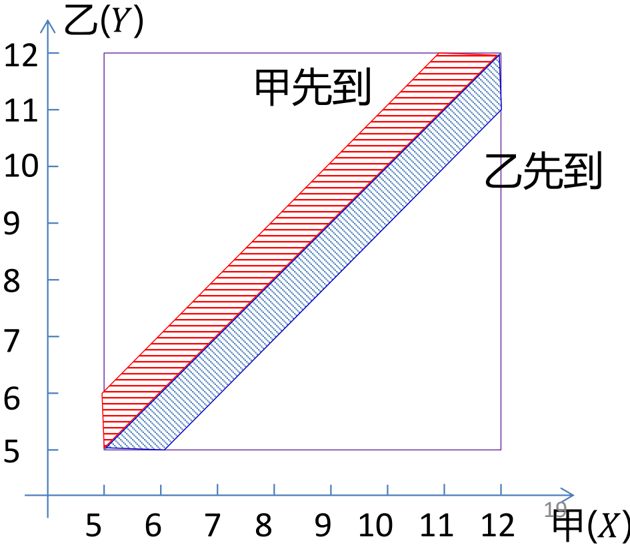
\includegraphics[width=0.5\textwidth]{figures/fig_meeting.png}
    \caption{会面问题示意图：正方形内 $|X-Y|\leq 1$ 的带状阴影区域}
    \label{fig:meeting}
\end{figure}

不满足条件的区域为两个直角三角形：
\begin{itemize}[leftmargin=2em]
    \item 上方三角形：顶点 $(0,1), (0,7), (6,7)$，直角边长 $6$；
    \item 下方三角形：顶点 $(1,0), (7,0), (7,6)$，直角边长 $6$。
\end{itemize}
每个三角形面积为 $\dfrac{1}{2} \times 6^2 = 18$，故不满足总面积为 $36$。满足条件的面积为
\[
m_A = 49 - 36 = 13.
\]
因此
\[
\boxed{P(\text{会面}) = \frac{13}{49}}.
\]

\subsubsection{蒲丰投针的几何概型解释}

\textbf{问题}：平面上有间距为 $d$（$d>0$）的平行线，向平面任意投掷长为 $l$（$l<d$）的针，求针与平行线相交的概率。

\textbf{解}：设 $x$ 为针中点 $M$ 到最近平行线的距离，$\theta$ 为针与平行线的交角。则样本空间为
\[
D = \left\{(\theta, x) \mid 0 \leq \theta \leq \pi,\; 0 \leq x \leq \frac{d}{2}\right\}, \quad m_D = \frac{d}{2} \cdot \pi.
\]
针与线相交的条件是中点到线距离不超过针在垂直方向投影的一半：
\[
x \leq \frac{l}{2}\sin\theta.
\]
故有利区域为
\[
A = \left\{(\theta, x) \mid 0 \leq \theta \leq \pi,\; 0 \leq x \leq \frac{l}{2}\sin\theta\right\}.
\]

\begin{figure}[htbp]
    \centering
    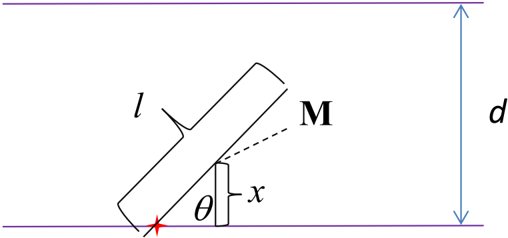
\includegraphics[width=0.6\textwidth]{figures/fig_buffon2.png}
    \caption{蒲丰投针几何概型示意图：针中点距离 $x$ 与夹角 $\theta$}
    \label{fig:buffon2}
\end{figure}

计算 $A$ 的面积：
\[
m_A = \int_0^\pi \frac{l}{2}\sin\theta \,\diff\theta = \frac{l}{2}[-\cos\theta]_0^\pi = \frac{l}{2}(1+1) = l.
\]
因此
\[
\boxed{P(\text{相交}) = \frac{m_A}{m_D} = \frac{l}{\frac{\pi d}{2}} = \frac{2l}{\pi d}}.
\]
若进行 $n$ 次投针，观察到 $m$ 次相交，则频率 $m/n \approx 2l/(\pi d)$，从而
\[
\boxed{\pi \approx \frac{2ln}{md}}.
\]

% ==================== §4 条件概率 ====================
\section{条件概率}

\subsection{引例}

\textbf{问题}：抛一枚硬币两次，$A$：至少出现一次正面；$B$：两次为同一面。求在 $A$ 发生的条件下 $B$ 发生的概率。

\textbf{解}：样本空间 $\Omega = \{HH, HT, TH, TT\}$。
\[
A = \{HH, HT, TH\}, \quad B = \{HH, TT\}, \quad A \cap B = \{HH\}.
\]
在 $A$ 已发生的条件下，样本空间缩小为 $A$，其中使 $B$ 发生的结果只有 $HH$。故
\[
P(B \mid A) = \frac{1}{3}.
\]

\subsection{条件概率的定义}

\begin{definition}[条件概率]
设 $A, B$ 是两个事件，且 $P(A) > 0$，称
\[
\boxed{P(B \mid A) = \frac{P(A \cap B)}{P(A)}}
\]
为在事件 $A$ 已发生的条件下事件 $B$ 发生的\textbf{条件概率}。
\end{definition}

\textbf{计算方法}：
\begin{enumerate}[label=(\arabic*),leftmargin=2em]
    \item \textbf{缩小样本空间法}：直接在新样本空间 $A$ 中计算 $B$ 发生的比例（适用于古典概型）；
    \item \textbf{公式法}：利用 $P(B \mid A) = P(AB)/P(A)$。
\end{enumerate}

\subsubsection{例1：乒乓球问题}

\textbf{问题}：盒中混有 $100$ 只新、旧乒乓球，各有黄、白两色，分布如下：
\[
\begin{array}{c|cc|c}
 & \text{黄} & \text{白} & \text{合计} \\ \hline
\text{新} & 40 & 30 & 70 \\
\text{旧} & 20 & 10 & 30 \\ \hline
\text{合计} & 60 & 40 & 100
\end{array}
\]
随机取出一球，若已知取得黄球，求该球是新球的概率。

\textbf{解}：设 $A$ = ``取出黄球''，$B$ = ``取出新球''。
\[
n_A = 60, \quad n_{A \cap B} = 40.
\]
由缩小样本空间法：
\[
\boxed{P(B \mid A) = \frac{n_{A \cap B}}{n_A} = \frac{40}{60} = \frac{2}{3}}.
\]
或由公式法：
\[
P(A) = \frac{60}{100} = \frac{3}{5}, \quad P(A \cap B) = \frac{40}{100} = \frac{2}{5}, \quad P(B \mid A) = \frac{2/5}{3/5} = \frac{2}{3}.
\]

\begin{figure}[htbp]
    \centering
    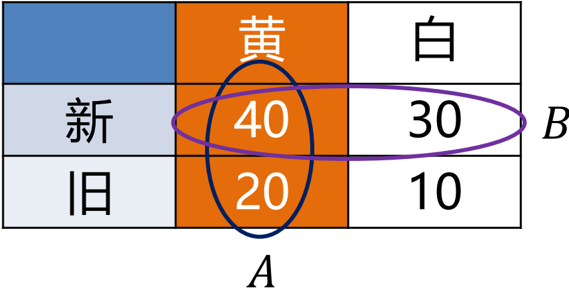
\includegraphics[width=0.4\textwidth]{figures/fig_conditional.png}
    \caption{条件概率示意图：事件 $A$ 中 $B$ 所占比例}
    \label{fig:conditional}
\end{figure}

\subsubsection{例2：有放回取球}

\textbf{问题}：盒中有 $4$ 个标号为 $1,2,3,4$ 的球，有放回地取两次。设 $B$ = ``两球标号之和为 $4$''。
\begin{enumerate}[label=(\arabic*),leftmargin=2em]
    \item 求 $P(B)$；
    \item 若已知第一次取出标号为 $2$（事件 $A$），求 $P(B \mid A)$。
\end{enumerate}

\textbf{解}：
\begin{enumerate}[label=(\arabic*),leftmargin=2em]
    \item 样本空间 $\Omega = \{(i,j) \mid i,j = 1,2,3,4\}$，共 $16$ 个样本点。
    \[
    B = \{(1,3), (2,2), (3,1)\}, \quad P(B) = \frac{3}{16}.
    \]
    
    \item $A = \{(2,1), (2,2), (2,3), (2,4)\}$。在 $A$ 发生条件下，样本空间缩小为 $4$ 个结果，其中只有 $(2,2) \in B$。故
    \[
    \boxed{P(B \mid A) = \frac{1}{4}}.
    \]
    注意：$P(B \mid A) = \dfrac{1}{4} \neq \dfrac{3}{16} = P(B)$，说明附加条件改变了概率。
\end{enumerate}

\subsection{条件概率是概率吗？}

条件概率 $P(\cdot \mid A)$ 满足概率的三条公理，因此它本身也是一种概率：

\begin{enumerate}[label=(\arabic*),leftmargin=2em]
    \item \textbf{非负性}：$P(B \mid A) \geq 0$；
    \item \textbf{规范性}：$P(\Omega \mid A) = \dfrac{P(\Omega \cap A)}{P(A)} = \dfrac{P(A)}{P(A)} = 1$；
    \item \textbf{可列可加性}：若 $B_1, B_2, \dots$ 两两互斥，则
    \[
    P\left(\bigcup_{i=1}^{\infty} B_i \,\middle|\, A\right) = \sum_{i=1}^{\infty} P(B_i \mid A).
    \]
\end{enumerate}

\begin{figure}[htbp]
    \centering
    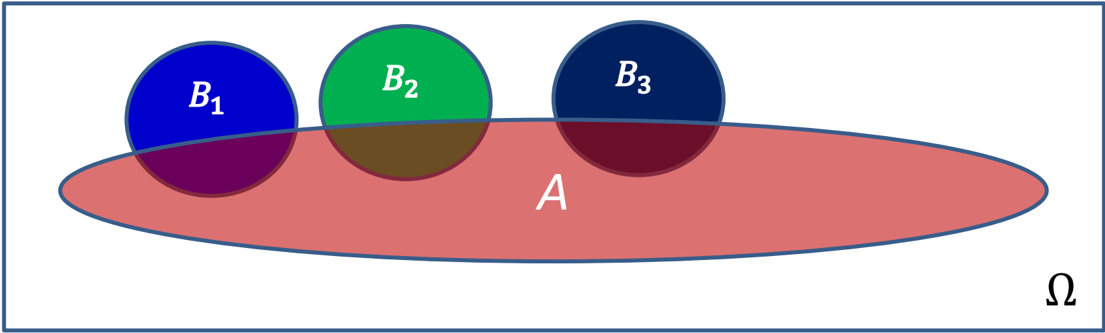
\includegraphics[width=0.7\textwidth]{figures/fig_conditional_additivity.png}
    \caption{条件概率的可列可加性示意图：$A$ 与互斥的 $B_i$ 的交集也互斥}
    \label{fig:conditional_additivity}
\end{figure}

由此可导出条件概率下的常用公式：

\begin{property}[逆事件公式]
\[
P(\bar{B} \mid A) = 1 - P(B \mid A).
\]
\end{property}

\begin{property}[加法公式]
对任意两事件 $B_1, B_2$，
\[
P(B_1 \cup B_2 \mid A) = P(B_1 \mid A) + P(B_2 \mid A) - P(B_1 \cap B_2 \mid A).
\]
\end{property}

\subsection{条件概率与无条件概率的关系}

\begin{note}
条件概率 $P(B \mid A)$ 与无条件概率 $P(B)$ 之间的大小\textbf{没有确定关系}。$P(B \mid A)$ 可能大于、等于或小于 $P(B)$，取决于事件 $A$ 与 $B$ 的具体关联。
\end{note}

\begin{figure}[htbp]
    \centering
    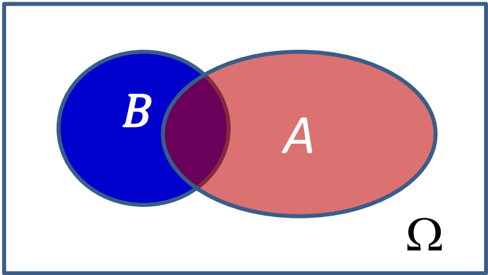
\includegraphics[width=0.5\textwidth]{figures/fig_cond_vs_uncond.png}
    \caption{条件概率与无条件概率的对比示意图：$|B|/|\Omega|$ vs $|A\cap B|/|A|$}
    \label{fig:cond_vs_uncond}
\end{figure}

\subsubsection{例3：市场占有率与合格率}

\textbf{问题}：市场上手机中，甲产品占有率 $50\%$，乙产品 $30\%$，其他品牌 $20\%$。甲、乙、其他品牌的合格率分别为 $95\%$、$80\%$、$60\%$。用 $A,B,C$ 分别表示甲、乙和其他品牌，$Q$ 表示合格品。

\textbf{已知}：
\[
\begin{aligned}
P(A) &= 0.5, & P(Q \mid A) &= 0.95, \\
P(B) &= 0.3, & P(Q \mid B) &= 0.8, \\
P(C) &= 0.2, & P(Q \mid C) &= 0.6.
\end{aligned}
\]

此例为后续全概率公式的应用做铺垫。

\subsubsection{例4：连续大雾问题}

\textbf{问题}：某地区连续两天出现清晨大雾的概率为 $0.1$，第一天大雾概率为 $0.6$，第二天大雾概率为 $0.3$。若游客第一天遇到大雾，求第二天没有大雾的概率。

\textbf{解}：设 $A_1, A_2$ 分别表示第一、第二天出现大雾。
\[
P(\bar{A}_2 \mid A_1) = \frac{P(A_1 \cap \bar{A}_2)}{P(A_1)} = \frac{P(A_1) - P(A_1 A_2)}{P(A_1)} = \frac{0.6 - 0.1}{0.6} = \boxed{\frac{5}{6}}.
\]

\subsection{乘法公式（乘法定理）}

由条件概率定义 $P(B \mid A) = \dfrac{P(AB)}{P(A)}$，直接得到：

\begin{theorem}[乘法公式]
对任意事件 $A, B \subset \Omega$，若 $P(A) > 0$，则
\[
\boxed{P(AB) = P(B \mid A) P(A)}.
\]
\end{theorem}

\textbf{推广到三事件}：设 $A,B,C$ 为三个事件，且 $P(AB) > 0$，则
\[
P(ABC) = P(C \mid AB) \cdot P(B \mid A) \cdot P(A).
\]

\textbf{一般情形}：设 $A_1, A_2, \dots, A_n$ 为 $n$ 个事件，且 $P(A_1 A_2 \cdots A_{n-1}) > 0$，则
\[
\boxed{P(A_1 A_2 \cdots A_n) = P(A_n \mid A_1 A_2 \cdots A_{n-1}) \cdot P(A_{n-1} \mid A_1 \cdots A_{n-2}) \cdots P(A_2 \mid A_1) \cdot P(A_1)}.
\]

\subsection{例5：波利亚罐子模型（P\'{o}lya's Urn Model / 传染模型）}

\textbf{模型设定}：盒中有 $r$ 个红球、$t$ 个白球。每次任取一球，观察颜色后放回，并再放入 $a$ 只与所取球颜色相同的球。连续取球 $4$ 次。

设 $A_i$ 表示第 $i$ 次取到红球，$\bar{A}_i$ 表示第 $i$ 次取到白球。

\begin{enumerate}[label=(\arabic*),leftmargin=2em]
    \item \textbf{第1、2次红球，第3、4次白球的概率}：
    \begin{align*}
    P(A_1 A_2 \bar{A}_3 \bar{A}_4) 
    &= P(\bar{A}_4 \mid A_1 A_2 \bar{A}_3) \cdot P(\bar{A}_3 \mid A_1 A_2) \cdot P(A_2 \mid A_1) \cdot P(A_1) \\
    &= \frac{t+a}{r+t+3a} \cdot \frac{t}{r+t+2a} \cdot \frac{r+a}{r+t+a} \cdot \frac{r}{r+t}.
    \end{align*}
    
    \item \textbf{第1、2次白球，第3、4次红球的概率}：
    \begin{align*}
    P(\bar{A}_1 \bar{A}_2 A_3 A_4) 
    &= P(A_4 \mid A_3 \bar{A}_2 \bar{A}_1) \cdot P(A_3 \mid \bar{A}_2 \bar{A}_1) \cdot P(\bar{A}_2 \mid \bar{A}_1) \cdot P(\bar{A}_1) \\
    &= \frac{r+a}{r+t+3a} \cdot \frac{r}{r+t+2a} \cdot \frac{t+a}{r+t+a} \cdot \frac{t}{r+t}.
    \end{align*}
\end{enumerate}

\textbf{一般公式}：在波利亚罐子模型中，先取出 $n_1$ 个红球，再取出 $n_2$ 个白球（总共 $n_1+n_2$ 次抽取），其概率为
\[
\boxed{p = \frac{r(r+a)\cdots(r+n_1 a - a) \cdot t(t+a)\cdots(t+n_2 a - a)}{(r+t)(r+t+a)\cdots(r+t+(n_1+n_2)a - a)}}.
\]

\begin{note}
波利亚模型是一种\textbf{ reinforced process（强化过程）}，常用于描述传染病的传播、品牌忠诚度等``富者愈富''现象。
\end{note}

% ==================== 全概率公式与Bayes公式 ====================
\subsection{样本空间的划分}

\begin{definition}[划分 / Partition]
设 $\Omega$ 为试验 $E$ 的样本空间，$B_1, B_2, \dots, B_n$ 为一组事件，若满足：
\begin{enumerate}[label=(\arabic*),leftmargin=2em]
    \item 两两互斥：$B_i \cap B_j = \varnothing,\; i \neq j,\; i,j = 1,2,\dots,n$；
    \item 完全覆盖：$\displaystyle\bigcup_{i=1}^{n} B_i = \Omega$，
\end{enumerate}
则称 $B_1, B_2, \dots, B_n$ 为样本空间 $\Omega$ 的一个\textbf{划分}（或完备事件组）。
\end{definition}

\textbf{特点}：对每次试验，有且仅有一个 $B_i$ 发生。

\textbf{例子}：掷骰子的两种划分：
\begin{itemize}[leftmargin=2em]
    \item $\{1,3,5\}, \{2,4,6\}$（按奇偶划分）；
    \item $\{1,2,3\}, \{4,5,6\}$（按大小划分）。
\end{itemize}

\begin{figure}[htbp]
    \centering
    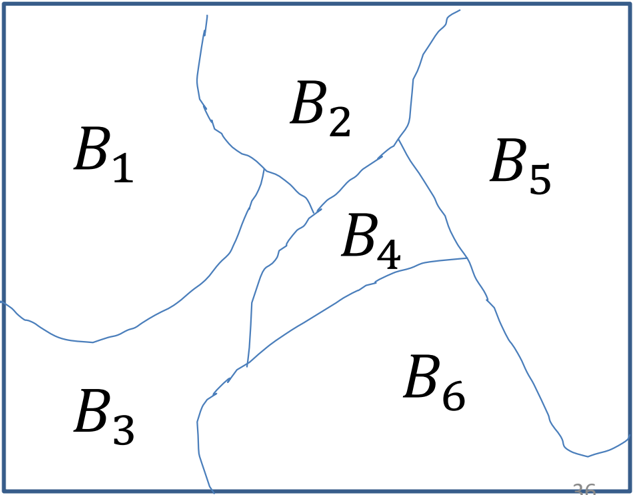
\includegraphics[width=0.5\textwidth]{figures/fig_partition.png}
    \caption{样本空间划分示意图：$B_1,B_2,\dots,B_6$ 构成 $\Omega$ 的一个划分}
    \label{fig:partition}
\end{figure}

\begin{figure}[htbp]
    \centering
    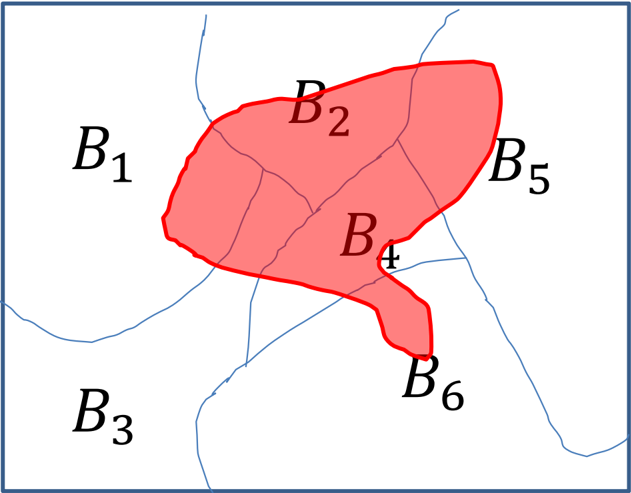
\includegraphics[width=0.5\textwidth]{figures/fig_partition_event.png}
    \caption{事件 $A$ 被划分切割：$A = \bigcup_{i} (A \cap B_i)$}
    \label{fig:partition_event}
\end{figure}

\subsection{全概率公式}

\begin{theorem}[全概率公式 / Law of Total Probability]
设试验 $E$ 的样本空间为 $\Omega$，$A$ 为 $E$ 的事件，$B_1, B_2, \dots, B_n$ 为 $\Omega$ 的一个划分，且 $P(B_i) > 0\;(i=1,2,\dots,n)$，则
\[
\boxed{P(A) = \sum_{i=1}^{n} P(A \mid B_i) P(B_i)}.
\]
\end{theorem}

\textbf{思想}：将复杂事件 $A$ 的概率分解到各个``原因'' $B_i$ 上分别计算，再求和。适用于直接计算 $P(A)$ 困难，但各分支条件概率已知的情形。

\subsubsection{例6：手机代工厂次品率}

\textbf{问题}：某品牌手机由甲、乙、丙三家代工厂生产，产量占比分别为 $1/4, 1/4, 1/2$，次品率分别为 $2\%, 1\%, 3\%$。求市场上该品牌手机的次品率。

\textbf{解}：设 $A_1, A_2, A_3$ 分别表示产品来自甲、乙、丙厂，$B$ 表示产品为次品。

\begin{figure}[htbp]
    \centering
    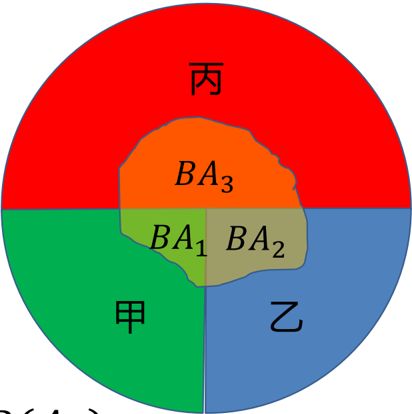
\includegraphics[width=0.5\textwidth]{figures/fig_phone_factory.png}
    \caption{手机代工厂问题示意图：三家工厂的市场份额与次品交集}
    \label{fig:phone_factory}
\end{figure}

由全概率公式：
\begin{align*}
P(B) &= P(B \mid A_1)P(A_1) + P(B \mid A_2)P(A_2) + P(B \mid A_3)P(A_3) \\
&= 0.02 \times \frac{1}{4} + 0.01 \times \frac{1}{4} + 0.03 \times \frac{1}{2} \\
&= 0.005 + 0.0025 + 0.015 = \boxed{0.0225}.
\end{align*}

\subsubsection{例7：两袋取球问题}

\textbf{问题}：甲袋中有 $2$ 个白球、$1$ 个红球；乙袋中有 $2$ 个红球、$1$ 个白球。这六个球手感不可区别。从甲袋任取一球放入乙袋，搅匀后再从乙袋任取一球，求取到红球的概率。

\textbf{解}：设 $A_1$ = ``从甲袋取出白球放入乙袋''，$A_2$ = ``从甲袋取出红球放入乙袋''，$B$ = ``从乙袋取到红球''。

先验概率：
\[
P(A_1) = \frac{2}{3}, \quad P(A_2) = \frac{1}{3}.
\]

条件概率：
\begin{itemize}[leftmargin=2em]
    \item 若 $A_1$ 发生（甲袋白球放入乙袋），乙袋变为 $2$ 红 $2$ 白，$P(B \mid A_1) = \dfrac{2}{4} = \dfrac{1}{2}$；
    \item 若 $A_2$ 发生（甲袋红球放入乙袋），乙袋变为 $3$ 红 $1$ 白，$P(B \mid A_2) = \dfrac{3}{4}$。
\end{itemize}

由全概率公式：
\[
P(B) = P(B \mid A_1)P(A_1) + P(B \mid A_2)P(A_2) = \frac{1}{2} \times \frac{2}{3} + \frac{3}{4} \times \frac{1}{3} = \frac{1}{3} + \frac{1}{4} = \boxed{\frac{7}{12}}.
\]

\subsection{乘法公式的拓展：已知结果求原因}

\textbf{续例7}：若已知从乙袋取到的是红球，求从甲袋放入乙袋的是白球的概率。

即求 $P(A_1 \mid B)$。由条件概率定义：
\[
P(A_1 \mid B) = \frac{P(A_1 B)}{P(B)} = \frac{P(B \mid A_1) P(A_1)}{P(B)} = \frac{\dfrac{1}{2} \times \dfrac{2}{3}}{\dfrac{7}{12}} = \frac{\dfrac{1}{3}}{\dfrac{7}{12}} = \boxed{\frac{4}{7}}.
\]

同理：
\[
P(A_2 \mid B) = \frac{P(B \mid A_2) P(A_2)}{P(B)} = \frac{\dfrac{3}{4} \times \dfrac{1}{3}}{\dfrac{7}{12}} = \frac{\dfrac{1}{4}}{\dfrac{7}{12}} = \frac{3}{7}.
\]

验证：$P(A_1 \mid B) + P(A_2 \mid B) = \dfrac{4}{7} + \dfrac{3}{7} = 1$。

% ==================== Bayes定理 ====================
\subsection{Bayes定理（贝叶斯公式）}

\begin{theorem}[Bayes公式]
设试验 $E$ 的样本空间为 $\Omega$，$A$ 为 $E$ 的一个事件，$B_1, B_2, \dots, B_n$ 为 $\Omega$ 的一个划分，且 $P(A) > 0,\; P(B_i) > 0\;(i=1,2,\dots,n)$，则对任意 $i$，
\[
\boxed{P(B_i \mid A) = \frac{P(A \mid B_i) P(B_i)}{\displaystyle\sum_{j=1}^{n} P(A \mid B_j) P(B_j)}}.
\]
\end{theorem}

\textbf{公式结构}：
\[
\underbrace{P(B_i \mid A)}_{\text{后验概率}} = \frac{\overbrace{P(A \mid B_i)}^{\text{似然}} \cdot \overbrace{P(B_i)}^{\text{先验}}}{\underbrace{\sum_{j=1}^{n} P(A \mid B_j) P(B_j)}_{\text{全概率 } P(A)}}.
\]

\begin{figure}[htbp]
    \centering
    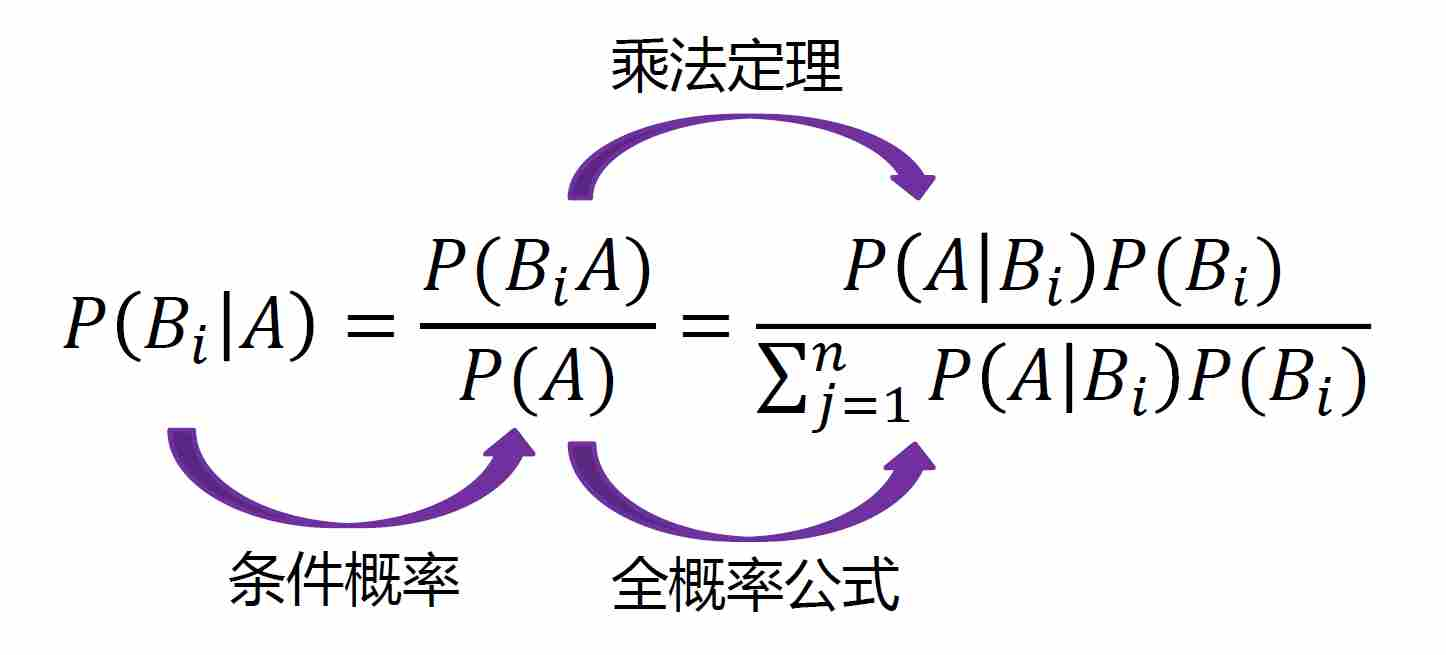
\includegraphics[width=0.7\textwidth]{figures/fig_bayes_cycle.png}
    \caption{Bayes公式的循环结构：条件概率 $\rightarrow$ 乘法定理 $\rightarrow$ 全概率公式}
    \label{fig:bayes_cycle}
\end{figure}

\textbf{两类事件的Bayes公式}（$n=2$ 的特例）：
\[
\begin{aligned}
P(A_1 \mid B) &= \frac{P(B \mid A_1) P(A_1)}{P(B \mid A_1) P(A_1) + P(B \mid A_2) P(A_2)}, \\[0.5em]
P(A_2 \mid B) &= \frac{P(B \mid A_2) P(A_2)}{P(B \mid A_1) P(A_1) + P(B \mid A_2) P(A_2)}.
\end{aligned}
\]

\subsubsection{例8：射手等级问题}

\textbf{问题}：某小组有 $20$ 名射手，其中一、二、三、四级射手分别为 $2,6,9,3$ 名。若选一、二、三、四级射手参赛，射中目标的概率分别为 $0.85, 0.64, 0.45, 0.32$。今随机选一人参赛。

\textbf{(1) 求该小组在比赛中射中目标的概率。}

\textbf{解}：设 $A$ = ``射中目标''，$B_i$ = ``选 $i$ 级选手''（$i=1,2,3,4$）。

先验概率：
\[
P(B_1) = \frac{2}{20} = 0.1,\; P(B_2) = \frac{6}{20} = 0.3,\; P(B_3) = \frac{9}{20} = 0.45,\; P(B_4) = \frac{3}{20} = 0.15.
\]

条件概率：
\[
P(A \mid B_1) = 0.85,\; P(A \mid B_2) = 0.64,\; P(A \mid B_3) = 0.45,\; P(A \mid B_4) = 0.32.
\]

由全概率公式：
\begin{align*}
P(A) &= 0.1 \times 0.85 + 0.3 \times 0.64 + 0.45 \times 0.45 + 0.15 \times 0.32 \\
&= 0.085 + 0.192 + 0.2025 + 0.048 = \boxed{0.5275}.
\end{align*}

\textbf{(2) 若已知射中目标，求该选手是一、二、三、四级选手的概率。}

由Bayes公式：
\[
\begin{aligned}
P(B_1 \mid A) &= \frac{0.085}{0.5275} \approx \boxed{0.1611}, \\
P(B_2 \mid A) &= \frac{0.192}{0.5275} \approx \boxed{0.3640}, \\
P(B_3 \mid A) &= \frac{0.2025}{0.5275} \approx \boxed{0.3839}, \\
P(B_4 \mid A) &= \frac{0.048}{0.5275} \approx \boxed{0.0910}.
\end{aligned}
\]

\textbf{先验与后验对比}：

\begin{table}[htbp]
\centering
\caption{先验概率与后验概率对比}
\begin{tabular}{@{}cccc@{}}
\toprule
\textbf{等级} & \textbf{先验} $P(B_i)$ & \textbf{后验} $P(B_i \mid A)$ & \textbf{条件概率} $P(A \mid B_i)$ \\
\midrule
一级 & $0.10$ & $0.1611$（$\uparrow$） & $0.85$ \\
二级 & $0.30$ & $0.3640$（$\uparrow$） & $0.64$ \\
三级 & $0.45$ & $0.3839$（$\downarrow$） & $0.45$ \\
四级 & $0.15$ & $0.0910$（$\downarrow$） & $0.32$ \\
\bottomrule
\end{tabular}
\end{table}

\begin{note}
观察到``射中目标''后，高等级选手（一、二级）的后验概率上升，低等级选手（三、四级）的后验概率下降。这是因为高等级选手的命中率更高，结果 $A$ 对他们更有利。
\end{note}

\subsubsection{例9：晶体管供应商问题}

\textbf{问题}：某电子设备制造厂所用晶体管由三家元件厂提供，数据如下：

\begin{table}[htbp]
\centering
\begin{tabular}{@{}ccc@{}}
\toprule
\textbf{元件厂} & \textbf{次品率} $P(A \mid B_i)$ & \textbf{市场份额} $P(B_i)$ \\
\midrule
1 & $0.02$ & $0.15$ \\
2 & $0.01$ & $0.80$ \\
3 & $0.03$ & $0.05$ \\
\bottomrule
\end{tabular}
\end{table}

三家产品在仓库中均匀混合且无区别标志。

\textbf{(1) 在仓库中随机取一只晶体管，求其次品率。}

\textbf{解}：设 $A$ = ``取到次品''，$B_i$ = ``取到第 $i$ 家工厂的产品''。

\begin{figure}[htbp]
    \centering
    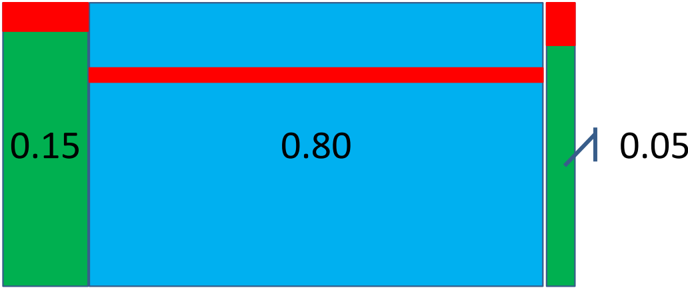
\includegraphics[width=0.6\textwidth]{figures/fig_transistor_share.png}
    \caption{晶体管供应商市场份额示意图}
    \label{fig:transistor_share}
\end{figure}

由全概率公式：
\[
P(A) = 0.02 \times 0.15 + 0.01 \times 0.80 + 0.03 \times 0.05 = 0.003 + 0.008 + 0.0015 = \boxed{0.0125}.
\]

\begin{figure}[htbp]
    \centering
    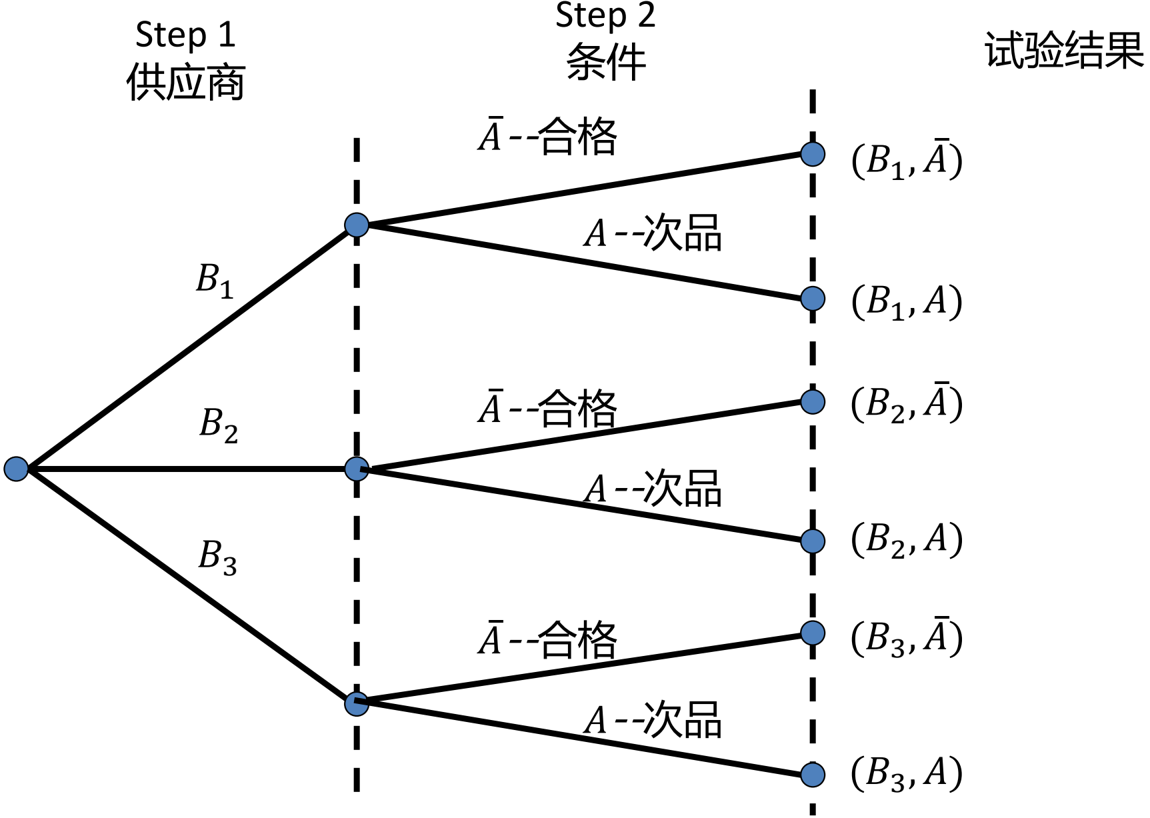
\includegraphics[width=0.7\textwidth]{figures/fig_total_prob_tree.png}
    \caption{全概率公式的树状图表示：Step 1 供应商 $\rightarrow$ Step 2 条件 $\rightarrow$ 试验结果}
    \label{fig:total_prob_tree}
\end{figure}

\begin{figure}[htbp]
    \centering
    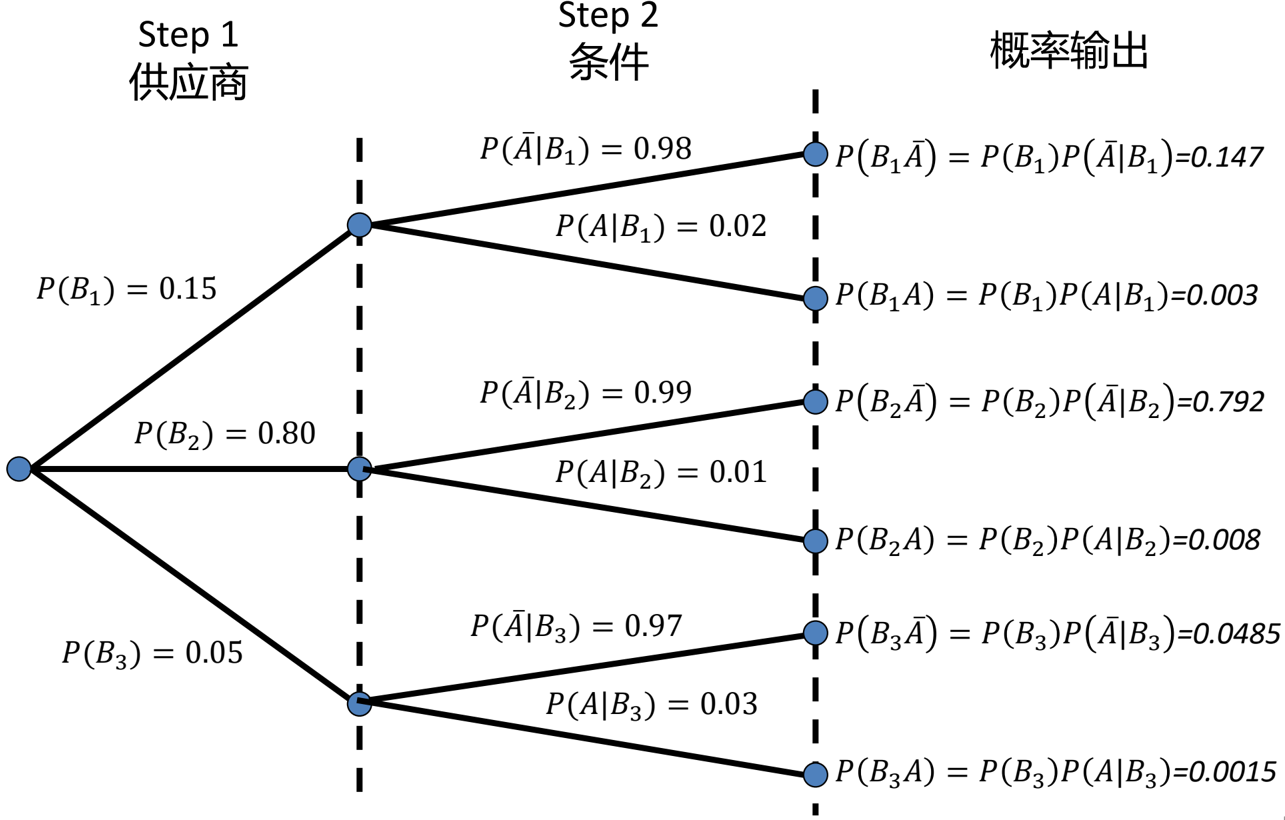
\includegraphics[width=0.8\textwidth]{figures/fig_prob_tree_numeric.png}
    \caption{树状图数值计算：各分支概率与联合概率}
    \label{fig:prob_tree_numeric}
\end{figure}

\textbf{(2) 若已知取到的是次品，求它出自各家工厂的概率。}

由Bayes公式：
\[
\begin{aligned}
P(B_1 \mid A) &= \frac{0.02 \times 0.15}{0.0125} = \frac{0.003}{0.0125} = \boxed{0.24}, \\
P(B_2 \mid A) &= \frac{0.01 \times 0.80}{0.0125} = \frac{0.008}{0.0125} = \boxed{0.64}, \\
P(B_3 \mid A) &= \frac{0.03 \times 0.05}{0.0125} = \frac{0.0015}{0.0125} = \boxed{0.12}.
\end{aligned}
\]

\begin{note}
虽然第3家工厂的次品率最高（$3\%$），但由于其市场份额极小（$5\%$），次品出自第3家的概率反而最低（$12\%$）。第2家工厂次品率最低（$1\%$），但因其占据 $80\%$ 市场，次品出自第2家的概率高达 $64\%$。
\end{note}

\subsection{Bayes公式的三种理解}

\subsubsection{理解1：从结果寻求关联因素}

\begin{itemize}[leftmargin=2em]
    \item 将事件 $A$ 看作某一过程的\textbf{结果}；
    \item 将 $B_1, B_2, \dots, B_n$ 看作导致该结果的\textbf{所有可能因素}；
    \item $P(B_i)$：根据历史信息得到的\textbf{先验概率}（Prior）；
    \item $P(A \mid B_i)$：每种因素对结果的影响程度，即\textbf{条件概率 / 似然}（Likelihood）；
    \item $P(B_i \mid A)$：事件 $A$ 已发生后，推断此事由第 $i$ 个因素引起的概率，即\textbf{后验概率}（Posterior）。
\end{itemize}

\begin{note}
Bayes公式本质上是发现\textbf{关联因素}，而非严格意义上的``原因''。统计关联不等于因果。
\end{note}

\subsubsection{理解2：组合先验知识与新信息修正预测}

\begin{figure}[htbp]
    \centering
    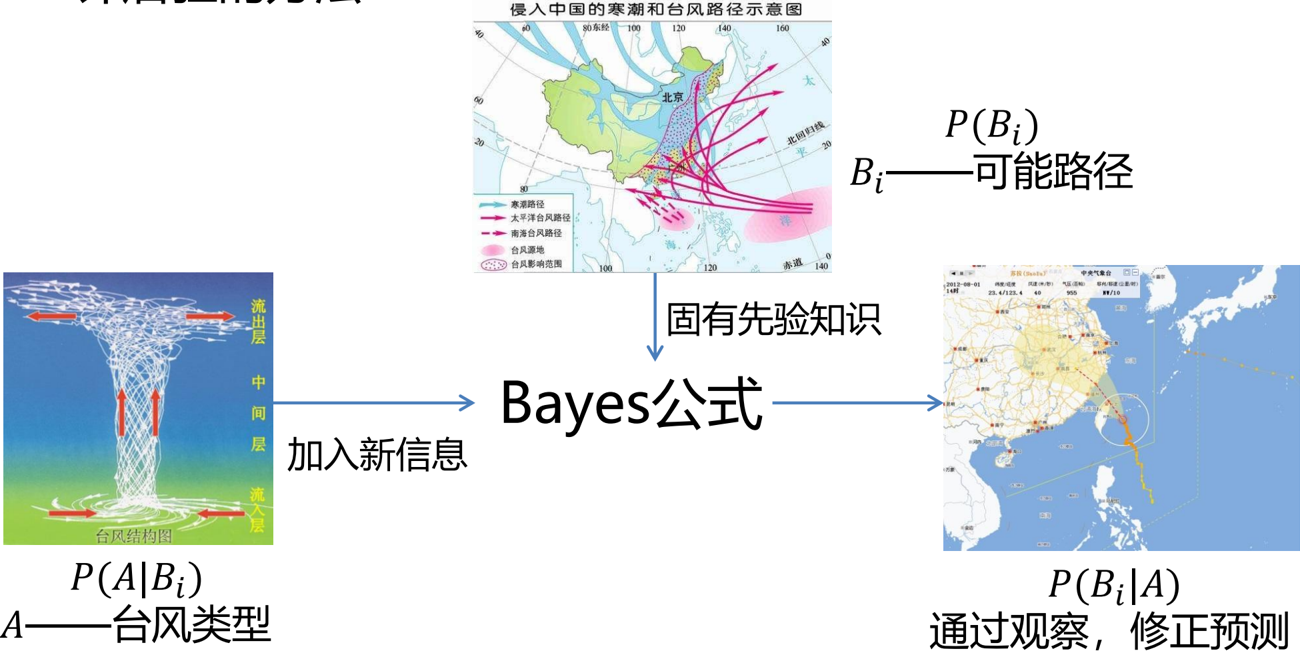
\includegraphics[width=0.9\textwidth]{figures/fig_bayes_typhoon.png}
    \caption{Bayes公式在台风路径预测中的应用：先验路径 $P(B_i)$ + 新观测 $P(A \mid B_i)$ $\rightarrow$ 修正预测 $P(B_i \mid A)$}
    \label{fig:bayes_typhoon}
\end{figure}

\textbf{应用场景}：气象预报、股票预测、导航定位等。先验知识（历史数据）与新观测信息结合，通过Bayes公式不断更新信念。

\subsubsection{理解3：建模因果关系，推断主要因素}

\begin{figure}[htbp]
    \centering
    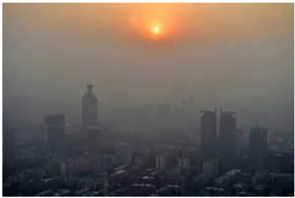
\includegraphics[width=0.9\textwidth]{figures/fig_bayes_smog.png}
    \caption{Bayes公式在雾霾成因分析中的应用：各种因素导致雾霾的模型 $P(A \mid B_i)$ + 先验 $P(B_i)$ $\rightarrow$ 判断主要因素 $P(B_i \mid A)$}
    \label{fig:bayes_smog}
\end{figure}

\textbf{核心思想}：建立``因素 $\rightarrow$ 结果''的因果模型（$P(A \mid B_i)$），结合各因素的先验发生概率，当观察到结果 $A$ 后，反推各因素的后验概率，从而判断主要影响因素。

\subsection{假阳性之谜（医学检测中的Bayes应用）}

\subsubsection{例10：疾病检测}

\textbf{问题}：某种检测方法对患病者的阳性率为 $0.95$（真阳性率），对非患病者的阴性率为 $0.96$（真阴性率）。人群中该疾病的发病率为 $0.001$。随机抽出一人，检出为阳性，求该人实际患病的概率。

\textbf{解}：设 $A$ = ``该人患病''，$B$ = ``该人检出为阳性''。

\begin{table}[htbp]
\centering
\caption{检测方法的性能指标}
\begin{tabular}{@{}lcc@{}}
\toprule
& \textbf{结果阳性} & \textbf{结果阴性} \\
\midrule
患病者 & $P(B \mid A) = 0.95$（真阳性） & $P(\bar{B} \mid A) = 0.05$（漏检率） \\
非患病者 & $P(B \mid \bar{A}) = 0.04$（误检率） & $P(\bar{B} \mid \bar{A}) = 0.96$（真阴性） \\
\bottomrule
\end{tabular}
\end{table}

由Bayes公式：
\[
P(A \mid B) = \frac{P(B \mid A) P(A)}{P(B \mid A) P(A) + P(B \mid \bar{A}) P(\bar{A})} = \frac{0.95 \times 0.001}{0.95 \times 0.001 + 0.04 \times 0.999} \approx \boxed{0.0232}.
\]

\begin{note}
\textbf{反直觉结论}：即使检出阳性，实际患病概率仅约 $2.32\%$！这是因为疾病发病率极低（$0.001$），大量健康人群中的误检（$4\%$）数量远超真实患者中的真检（$95\%$）。$P(B \mid A)$ 远不能代表 $P(A \mid B)$，不必被检查结果吓坏。
\end{note}

\textbf{追问}：若检出阴性，是否安全？

\[
P(\bar{A} \mid \bar{B}) = \frac{P(\bar{B} \mid \bar{A}) P(\bar{A})}{P(\bar{B} \mid A) P(A) + P(\bar{B} \mid \bar{A}) P(\bar{A})} = \frac{0.96 \times 0.999}{0.05 \times 0.001 + 0.96 \times 0.999} \approx \boxed{0.9999479}.
\]

检出阴性后，确实安全的概率极高（约 $99.995\%$），安全程度比单纯的真阴性率 $P(\bar{B} \mid \bar{A}) = 0.96$ 大幅提升。

% ==================== §4 补充：Bayes 方法注释 ====================
\subsection{关于 Bayes 方法的一些注释}

\textbf{Thomas Bayes}（1702--1763）：18 世纪英国神学家、数学家、数理统计学家、哲学家、牧师。他关注将\textbf{先验知识}融于概率计算，其方法可广泛用于各种参数估计。

\textbf{Bayes 主义与频率主义的分歧}：

\begin{table}[htbp]
\centering
\caption{频率主义与 Bayes 主义的对比}
\begin{tabular}{@{}lll@{}}
\toprule
\textbf{维度} & \textbf{频率主义（Frequentist）} & \textbf{Bayes 主义（Bayesian）} \\
\midrule
参数性质 & 参数是固定常数，非随机 & 参数是随机变量，有分布 \\
区间估计 & 置信区间（Confidence Interval） & 通过后验分布构造可信区间 \\
先验知识 & 不引入主观先验 & 必须引入先验分布 $P(B_i)$ \\
\bottomrule
\end{tabular}
\end{table}

\begin{note}
频率主义者的核心疑问：先验知识往往带有\textbf{偏差和主观性}，如何确保其客观性？现代统计中，两种方法各有适用场景，且在大数据条件下后验往往受数据主导，先验影响减弱。
\end{note}

\begin{figure}[htbp]
    \centering
    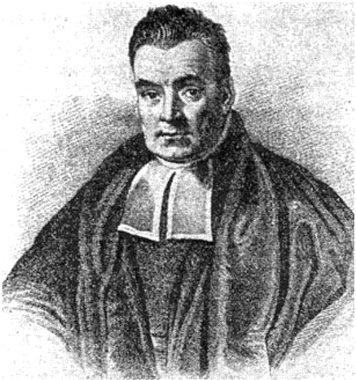
\includegraphics[width=0.3\textwidth]{figures/fig_bayes_portrait.png}
    \caption{Thomas Bayes 肖像}
    \label{fig:bayes_portrait}
\end{figure}

% ==================== §5 独立性 ====================
\section{独立性}

\subsection{引例：有放回取球}

\textbf{例1}：袋中有 $a$ 只黑球、$b$ 只白球。每次取出一球后\textbf{放回}。令
\[
A = \{\text{第一次取出白球}\}, \quad B = \{\text{第二次取出白球}\}.
\]
求 $P(B)$ 与 $P(B \mid A)$。

\textbf{解}：
\[
P(A) = \frac{b}{a+b}, \quad P(AB) = \left(\frac{b}{a+b}\right)^2, \quad P(\bar{A}B) = \frac{ab}{(a+b)^2}.
\]
由 $B = AB \cup \bar{A}B$（两者互斥），得
\[
P(B) = P(AB) + P(\bar{A}B) = \frac{b^2}{(a+b)^2} + \frac{ab}{(a+b)^2} = \frac{b}{a+b}.
\]
而
\[
P(B \mid A) = \frac{P(AB)}{P(A)} = \frac{b^2/(a+b)^2}{b/(a+b)} = \frac{b}{a+b}.
\]

\textbf{结论}：$P(B) = P(B \mid A)$。事件 $A$ 是否发生对事件 $B$ 的概率没有影响。

\begin{note}
由于是有放回摸球，第二次取球时袋中球的总数与黑白比例均未改变，因此第二次摸出白球的概率自然不变。
\end{note}

\subsection{事件独立性的定义}

\begin{definition}[两事件独立]
设 $A, B$ 是两个随机事件，如果满足
\[
\boxed{P(AB) = P(A)P(B)},
\]
则称 $A$ 与 $B$ \textbf{相互独立}。
\end{definition}

\begin{theorem}[独立性的等价刻画]
若事件 $A$ 与 $B$ 相互独立，且 $P(A) > 0$，则
\[
P(B \mid A) = P(B).
\]
\end{theorem}

\begin{proof}
由独立性 $P(AB) = P(A)P(B)$，故
\[
P(B \mid A) = \frac{P(AB)}{P(A)} = \frac{P(A)P(B)}{P(A)} = P(B).
\]
\end{proof}

\begin{theorem}[平凡事件的独立性]
必然事件 $\Omega$ 与任意随机事件 $A$ 相互独立；不可能事件 $\varnothing$ 与任意随机事件 $A$ 相互独立。
\end{theorem}

\begin{proof}
\[
P(\Omega A) = P(A) = 1 \cdot P(A) = P(\Omega)P(A).
\]
\[
P(\varnothing A) = P(\varnothing) = 0 = P(\varnothing)P(A).
\]
\end{proof}

\begin{theorem}[独立性的对偶性]
若随机事件 $A$ 与 $B$ 相互独立，则下列各对事件也相互独立：
\[
A \text{ 与 } \bar{B}, \quad \bar{A} \text{ 与 } B, \quad \bar{A} \text{ 与 } \bar{B}.
\]
\end{theorem}

\begin{proof}
由于 $A = A(B \cup \bar{B}) = AB \cup A\bar{B}$，且 $AB$ 与 $A\bar{B}$ 互斥，故
\[
P(A) = P(AB) + P(A\bar{B}) = P(A)P(B) + P(A\bar{B}).
\]
于是
\[
P(A\bar{B}) = P(A) - P(A)P(B) = P(A)\bigl(1-P(B)\bigr) = P(A)P(\bar{B}).
\]
故 $A$ 与 $\bar{B}$ 独立。同理可证 $\bar{A}$ 与 $B$ 独立。在此基础上，利用 $\bar{\bar{B}} = B$ 即得 $\bar{A}$ 与 $\bar{B}$ 独立。
\end{proof}

\subsection{互不相容与相互独立的关系}

设事件 $A$ 与 $B$ 满足 $P(A) > 0,\; P(B) > 0$，则：

\begin{enumerate}[label=(\arabic*),leftmargin=2em]
    \item 若 $A$ 与 $B$ 相互独立，则 $AB \neq \varnothing$（即不互斥）；
    \item 若 $AB = \varnothing$（互斥），则 $A$ 与 $B$ 不相互独立。
\end{enumerate}

\begin{proof}
\begin{enumerate}[label=(\arabic*),leftmargin=1em]
    \item 由独立性，$P(AB) = P(A)P(B) > 0$，故 $AB \neq \varnothing$。
    \item 由互斥性，$P(AB) = P(\varnothing) = 0$，但 $P(A)P(B) > 0$，故 $P(AB) \neq P(A)P(B)$，不独立。
\end{enumerate}
\end{proof}

\begin{note}
当 $A, B$ 均为非空事件时，\textbf{互不相容}与\textbf{相互独立}不能同时成立。互斥意味着``有你没我''（强排斥），独立意味着``互不影响''（无关联），二者逻辑上矛盾。
\end{note}

\subsection{不独立事件的例子：不放回取球}

\textbf{例2}：袋中有 $a$ 只黑球、$b$ 只白球。每次取出一球后\textbf{不放回}。令
\[
A = \{\text{第一次取出白球}\}, \quad B = \{\text{第二次取出白球}\}.
\]
求 $P(B)$ 与 $P(B \mid A)$。

\textbf{解}：
\[
P(A) = \frac{b}{a+b}, \quad P(AB) = \frac{b(b-1)}{(a+b)(a+b-1)}, \quad P(\bar{A}B) = \frac{ab}{(a+b)(a+b-1)}.
\]
于是
\[
P(B) = P(AB) + P(\bar{A}B) = \frac{b(b-1)+ab}{(a+b)(a+b-1)} = \frac{b}{a+b}.
\]
而
\[
P(B \mid A) = \frac{P(AB)}{P(A)} = \frac{b-1}{a+b-1}.
\]
显然 $P(B \mid A) \neq P(B)$（除非 $a=0$）。

\begin{note}
不放回抽样时，第一次取球改变了袋中球的组成，第二次取球的条件分布已不同于无条件分布，因此 $A$ 与 $B$ 不独立。
\end{note}

\subsection{实际问题中的独立性判断}

\begin{itemize}[leftmargin=2em]
    \item 实际应用中，往往难以从数学定义直接验证独立性，而是根据\textbf{实际意义}（物理机制、试验设计）加以判断。
    \item 在习题中，一般将独立性作为\textbf{已知条件}直接给出。
\end{itemize}

\subsection{独立性推广——三事件}

\begin{definition}[三事件相互独立]
设 $A, B, C$ 是三个随机事件，如果满足
\[
\begin{cases}
P(AB) = P(A)P(B), \\[0.3em]
P(BC) = P(B)P(C), \\[0.3em]
P(AC) = P(A)P(C), \\[0.3em]
P(ABC) = P(A)P(B)P(C),
\end{cases}
\]
则称 $A, B, C$ \textbf{相互独立}。
\end{definition}

\begin{warning}
四个等式\textbf{缺一不可}：
\begin{itemize}[leftmargin=2em]
    \item 前三个等式（两两独立）\textbf{不能推出}第四个等式；
    \item 第四个等式也\textbf{不能推出}前三个等式。
\end{itemize}
\end{warning}

\subsubsection{两两独立但三事件不独立的经典反例}

\textbf{反例1（字母排列）}：考虑字母 $a,b,c$ 的全部 $6$ 个排列，再加上 $3$ 个三元组 $(a,a,a), (b,b,b), (c,c,c)$，共 $9$ 个样本点构成样本空间，赋均匀概率 $1/9$。

令 $A_k$ 表示``字母 $a$ 出现在第 $k$ 个位置''（$k=1,2,3$）。则
\[
P(A_1) = P(A_2) = P(A_3) = \frac{3}{9} = \frac{1}{3}.
\]
两两交集（如 $A_1 \cap A_2$ 只有 $(a,a,a)$ 一个样本点）：
\[
P(A_1A_2) = P(A_2A_3) = P(A_1A_3) = \frac{1}{9} = P(A_1)P(A_2).
\]
故三者\textbf{两两独立}。但
\[
P(A_1A_2A_3) = \frac{1}{9} \neq \frac{1}{27} = P(A_1)P(A_2)P(A_3).
\]
因此\textbf{不相互独立}。

\textbf{反例2（涂色球）}：袋中有 $4$ 个外形相同的球，其中三个分别涂有红、白、黑色，另一个涂有红、白、黑三种颜色。任取一球，令
\[
A = \{\text{涂有红色}\},\; B = \{\text{涂有白色}\},\; C = \{\text{涂有黑色}\}.
\]
则
\[
P(A) = P(B) = P(C) = \frac{2}{4} = \frac{1}{2}.
\]
\[
P(AB) = P(BC) = P(AC) = \frac{1}{4} = P(A)P(B).
\]
但 $ABC$ 对应取到三色球，$P(ABC) = \dfrac{1}{4} \neq \dfrac{1}{8} = P(A)P(B)P(C)$。

\subsection{独立性推广——\texorpdfstring{$n$}{n} 事件}

\begin{definition}[$n$ 事件相互独立]
设 $A_1, A_2, \dots, A_n$ 是 $n$ 个随机事件，如果对所有可能的 $2 \leq m \leq n$ 及任意 $1 \leq i_1 < i_2 < \dots < i_m \leq n$，都有
\[
P(A_{i_1}A_{i_2}\cdots A_{i_m}) = P(A_{i_1})P(A_{i_2})\cdots P(A_{i_m}),
\]
则称 $A_1, A_2, \dots, A_n$ \textbf{相互独立}。
\end{definition}

\textbf{等式个数}：第 $m$ 层有 $\dbinom{n}{m}$ 个等式，总等式数为
\[
\sum_{m=2}^{n} \dbinom{n}{m} = 2^n - \dbinom{n}{0} - \dbinom{n}{1} = \boxed{2^n - n - 1}.
\]

\subsection{独立随机事件的性质及应用}

\begin{theorem}[独立事件组的子集独立性]
若 $A_1, A_2, \dots, A_n$ 相互独立，则将其任意部分事件改为对立事件后，所得的 $n$ 个事件仍然相互独立。
\end{theorem}

\textbf{独立事件至少发生其一的概率}：

若 $A_1, A_2, \dots, A_n$ 相互独立，则
\[
P(A_1 \cup A_2 \cup \cdots \cup A_n) = 1 - P(\bar{A}_1\bar{A}_2\cdots\bar{A}_n) = 1 - P(\bar{A}_1)P(\bar{A}_2)\cdots P(\bar{A}_n).
\]

若 $P(A_i) = p$（常数），则
\[
P(A_1 \cup A_2 \cup \cdots \cup A_n) = 1 - (1-p)^n.
\]

\begin{note}
只要 $p < 1$，当 $n \to \infty$ 时，
\[
\lim_{n\to\infty} P(A_1 \cup A_2 \cup \cdots \cup A_n) = 1.
\]
此即\textbf{小概率事件终究要发生}：即使单次概率很小，只要重复次数足够多，至少发生一次的概率趋于 $1$。
\end{note}

\subsubsection{例4：电路继电器问题}

\textbf{问题}：设有电路如图，其中 $1,2,3,4$ 为继电器接点。各继电器接点闭合与否相互独立，且每个接点闭合的概率均为 $p$。求 $L$ 至 $R$ 为通路的概率。

\begin{figure}[htbp]
    \centering
    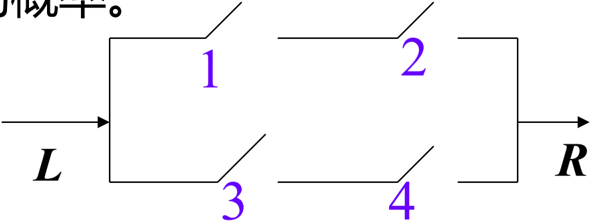
\includegraphics[width=0.5\textwidth]{figures/fig_circuit.png}
    \caption{电路继电器示意图：并联串联结构}
    \label{fig:circuit}
\end{figure}

\textbf{解}：设 $A_i$ 表示第 $i$ 个继电器接点闭合（$i=1,2,3,4$）。$L$ 至 $R$ 通路可表示为
\[
A = A_1A_2 \cup A_3A_4.
\]
由加法公式与独立性：
\begin{align*}
P(A) &= P(A_1A_2) + P(A_3A_4) - P(A_1A_2A_3A_4) \\
&= P(A_1)P(A_2) + P(A_3)P(A_4) - P(A_1)P(A_2)P(A_3)P(A_4) \\
&= p^2 + p^2 - p^4 = \boxed{2p^2 - p^4}.
\end{align*}

\subsubsection{例5：乐器验收问题}

\textbf{问题}：验收一批 $100$ 件乐器。方案：随机抽取 $3$ 件测试（测试相互独立）。若至少有一件被测为音色不纯，则拒收。设一件音色不纯的乐器被测出的概率为 $0.95$，一件音色纯的乐器被误测为不纯的概率为 $0.01$。若这批乐器中恰有 $4$ 件音色不纯，求被接受的概率。

\textbf{解}：设 $H_i$ 表示抽出的 $3$ 件中恰有 $i$ 件音色不纯（$i=0,1,2,3$），$A$ 表示这批乐器被接受（即 $3$ 件都被测为音色纯）。

\textbf{Step 1：先验概率}（超几何分布）
\[
\begin{aligned}
P(H_0) &= \frac{\dbinom{96}{3}}{\dbinom{100}{3}}, &
P(H_1) &= \frac{\dbinom{4}{1}\dbinom{96}{2}}{\dbinom{100}{3}}, \\
P(H_2) &= \frac{\dbinom{4}{2}\dbinom{96}{1}}{\dbinom{100}{3}}, &
P(H_3) &= \frac{\dbinom{4}{3}}{\dbinom{100}{3}}.
\end{aligned}
\]

\textbf{Step 2：条件概率}（测试独立性）
\begin{itemize}[leftmargin=2em]
    \item 若 $H_0$（3件均纯）：每件被正确判纯的概率 $0.99$，故 $P(A \mid H_0) = 0.99^3$；
    \item 若 $H_1$（1件不纯，2件纯）：不纯件被漏检（判纯）概率 $1-0.95=0.05$，纯件被正确判纯概率 $0.99$，故 $P(A \mid H_1) = 0.99^2 \times 0.05$；
    \item 若 $H_2$（2件不纯，1件纯）：$P(A \mid H_2) = 0.99 \times 0.05^2$；
    \item 若 $H_3$（3件均不纯）：$P(A \mid H_3) = 0.05^3$。
\end{itemize}

\textbf{Step 3：全概率公式}
\[
P(A) = \sum_{i=0}^{3} P(A \mid H_i) P(H_i) \approx \boxed{0.8629}.
\]

\subsection{\texorpdfstring{$n$}{n} 重 Bernoulli 概型}

\subsubsection{Bernoulli 试验}

\begin{definition}[Bernoulli 试验]
若随机试验 $E$ 只有两个结果，则称 $E$ 为\textbf{Bernoulli 试验}。通常将两个结果分别记为 $A$（``成功''）与 $\bar{A}$（``失败''）。
\end{definition}

\textbf{例子}：
\begin{itemize}[leftmargin=2em]
    \item 掷一枚硬币（正面/反面）；
    \item 掷一颗骰子，只关心``出现6点''与``不出现6点''；
    \item 对同一目标射击一次（击中/未击中）；
    \item 观察某路口汽车数，只关心``至少通过100辆''与``至多通过99辆''。
\end{itemize}

\subsubsection{\texorpdfstring{$n$}{n} 重 Bernoulli 试验}

\begin{definition}
若\textbf{独立重复}地进行 $n$ 次 Bernoulli 试验，其中``重复''指每次 $P(A)=p$ 不变，``独立''指各次结果互不影响，则称该试验为\textbf{$n$ 重 Bernoulli 试验}。
\end{definition}

\textbf{例子}：
\begin{itemize}[leftmargin=2em]
    \item 掷 $n$ 次硬币；
    \item 掷 $n$ 颗骰子，每颗只关心是否出6点；
    \item 对同一目标进行 $n$ 次独立射击；
    \item 独立重复 $n$ 次观察某路口汽车数。
\end{itemize}

\subsubsection{二项分布公式}

在 $n$ 重 Bernoulli 试验中，设 $P(A)=p,\; P(\bar{A})=q=1-p$。令 $B_{n,k}$ 表示``事件 $A$ 恰好发生 $k$ 次''，则

\textbf{指定位置}：若指定某 $k$ 次成功、其余 $n-k$ 次失败，由独立性其概率为 $p^k q^{n-k}$。

\textbf{任意位置}：$k$ 次成功可出现在 $\dbinom{n}{k}$ 种不同位置，故
\[
\boxed{P(B_{n,k}) = \dbinom{n}{k} p^k q^{n-k}, \quad k=0,1,2,\dots,n}.
\]

\textbf{规范性}：由二项式定理
\[
\sum_{k=0}^{n} P(B_{n,k}) = \sum_{k=0}^{n} \dbinom{n}{k} p^k q^{n-k} = (p+q)^n = 1.
\]

\subsubsection{例6：产品次品率}

\textbf{问题}：一大批产品次品率为 $0.05$，现从中取 $10$ 件。求：
\begin{itemize}[leftmargin=2em]
    \item $B$：恰有 $4$ 件次品；
    \item $C$：至少有 $2$ 件次品；
    \item $D$：没有次品。
\end{itemize}

\textbf{解}：设 $A$ = ``取出1件为次品''，则 $P(A)=0.05$。取 $10$ 件可看作 $10$ 重 Bernoulli 试验。

\begin{align*}
P(B) &= \dbinom{10}{4} \times 0.05^4 \times 0.95^6 \approx 9.648 \times 10^{-4}, \\
P(C) &= 1 - P(\bar{C}) = 1 - \dbinom{10}{0}0.05^0 0.95^{10} - \dbinom{10}{1}0.05^1 0.95^9 \\
&= 1 - 0.95^{10} - 10 \times 0.05 \times 0.95^9 \approx \boxed{0.0861}, \\
P(D) &= 0.95^{10} \approx \boxed{0.5987}.
\end{align*}

% ==================== 作业 ====================
\section*{作业}

\addcontentsline{toc}{section}{作业}

\subsection*{教材《概率论及其应用》}
\begin{enumerate}[label=\arabic*.,leftmargin=2em]
    \item 1.8（p.20/21）：\#14, \#16, \#17, \#19
    \item 2.10（pp.42--44 / 45--47）：\#9, \#11, \#21, \#24, \#38
    \item 5.8（pp.107--109 / 116--118）：\#6, \#7, \#18, \#19, \#26
    \item 6.10（p.129 / 139）：\#5, \#12, \#16
\end{enumerate}

\subsection*{教材《概率论与数理统计》（盛聚等）}
\begin{enumerate}[label=\arabic*.,leftmargin=2em]
    \item 第一章（pp.25--29）：\#2, \#8, \#12, \#13, \#16, \#18, \#19, \#23, \#25, \#26, \#29, \#33, \#35, \#38
\end{enumerate}

\newpage
\chapter{随机变量及其分布}

\section{随机变量}

\subsection{随机变量的概念}

\begin{example}[摸球问题]
袋中有3只黑球，2只白球，从中任意取出3只球，观察取出的3只球中的黑球个数。将3只黑球分别记作1,2,3号，2只白球分别记作4,5号，则该试验的样本空间为
\[
\Omega = \{(1,2,3), (1,2,4), (1,2,5), (1,3,4), (1,3,5), (1,4,5), (2,3,4), (2,3,5), (2,4,5), (3,4,5)\}.
\]
记取出的黑球数为 $X$，则 $X$ 的可能取值为 $1,2,3$。$X$ 的取值依赖于试验结果，带有随机性，故称 $X$ 为\textbf{随机变量}。
\end{example}

\begin{definition}[随机变量]
设 $E$ 是一个随机试验，$\Omega$ 是其样本空间。若对每一个 $\omega \in \Omega$，都有唯一确定的一个实数 $X(\omega)$ 与之对应，则称 $X(\omega)$ 为一个\textbf{随机变量}。
\end{definition}

\begin{figure}[htbp]
    \centering
    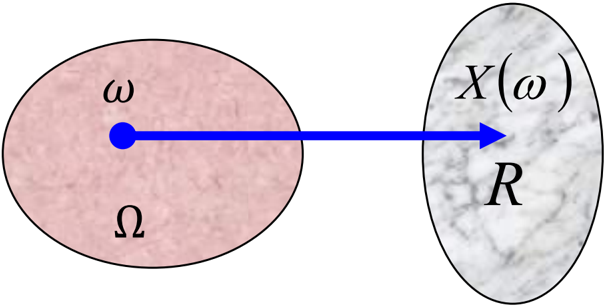
\includegraphics[width=0.5\textwidth]{figures/fig_rv_mapping.png}
    \caption{样本空间到实数的映射示意图}
    \label{fig:rv_mapping}
\end{figure}

\begin{note}
\begin{itemize}[leftmargin=2em]
    \item 随机变量常用大写英文字母 $X,Y,Z$ 或希腊字母 $\xi,\eta,\zeta$ 等来表示。
    \item 对于随机变量，关心其取值：试验前可以知道它的所有可能结果，但不确定取什么值。
\end{itemize}
\end{note}

\begin{example}[例1续]
定义了随机变量后，就可以用随机变量的取值情况来刻画随机事件。例如
\[
\{X=2\} = \{(1,2,4), (1,2,5), (1,3,4), (1,3,5), (2,3,4), (2,3,5)\}
\]
表示取出2个黑球这一事件。又如
\[
\{X \geq 2\} = \{X=2\} \cup \{X=3\}
\]
表示至少取出2个黑球这一事件。
\end{example}

\begin{example}[掷骰子]
掷一颗骰子，令 $X$ 表示出现的点数，则 $X$ 就是一个随机变量，取值为 $1,2,3,4,5,6$。
\begin{itemize}[leftmargin=2em]
    \item $\{X \geq 4\} = \{4,5,6\}$ 表示掷出的点数不小于4；
    \item $\{X \text{ 取偶数}\} = \{2,4,6\}$ 表示掷出的点数为偶数。
\end{itemize}
\end{example}

\begin{example}[产品抽样]
一批产品有50件，其中有8件次品，42件正品。现从中取出6件，令 $X$ 表示取出6件产品中的次品数，则 $X$ 就是一个随机变量，取值为 $0,1,2,\dots,6$。
\begin{itemize}[leftmargin=2em]
    \item $\{X=0\}$ 表示取出的产品全是正品；
    \item $\{X \geq 1\}$ 表示取出的产品中至少有一件次品。
\end{itemize}
\end{example}

\begin{example}[车流量观察]
上午 $8{:}00 \sim 9{:}00$ 在某路口观察，令 $Y$ 表示该时间间隔内通过的汽车数，则 $Y$ 就是一个随机变量，取值为 $0,1,2,\dots$（可列无穷个）。
\begin{itemize}[leftmargin=2em]
    \item $\{Y < 100\}$ 表示通过的汽车数小于100辆；
    \item $\{50 < Y < 100\}$ 表示通过的汽车数大于50辆但不超过100辆。
\end{itemize}
\end{example}

\begin{example}[寿命观察]
观察某生物的寿命（单位：小时），令 $Z$ 表示该生物的寿命，则 $Z$ 就是一个随机变量，取值为所有非负实数（不可列无穷个）。
\begin{itemize}[leftmargin=2em]
    \item $\{Z < 1500\}$ 表示该生物的寿命不超过1500小时；
    \item $\{Z > 3000\}$ 表示该生物的寿命大于3000小时。
\end{itemize}
\end{example}

\begin{example}[同一样本空间上的不同随机变量]
掷一枚骰子，在例2中定义了随机变量 $X$ 表示出现的点数。还可以定义其他随机变量，例如
\[
Y = \begin{cases} 1, & \text{掷出偶数}, \\ 0, & \text{掷出奇数}, \end{cases} \qquad
Z = \begin{cases} 1, & \text{点数} \geq 4, \\ 0, & \text{点数} < 4. \end{cases}
\]
\end{example}

\section{离散型随机变量}

\subsection{离散型随机变量的概念与性质}

\begin{definition}[离散型随机变量]
如果随机变量 $X$ 的取值是有限个或可列无穷个，则称 $X$ 为\textbf{离散型随机变量}。
\end{definition}

\begin{definition}[分布律]
设离散型随机变量 $X$ 的所有可能取值为 $x_1, x_2, \dots, x_k, \dots$，并设
\[
P\{X = x_k\} = p_k, \quad k=1,2,\dots
\]
则称上式为离散型随机变量 $X$ 的\textbf{分布律}。

离散型随机变量 $X$ 的分布律还可列成下表：
\begin{table}[htbp]
\centering
\begin{tabular}{@{}cccccc@{}}
\toprule
$X$ & $x_1$ & $x_2$ & $\cdots$ & $x_k$ & $\cdots$ \\
\midrule
$P$ & $p_1$ & $p_2$ & $\cdots$ & $p_k$ & $\cdots$ \\
\bottomrule
\end{tabular}
\end{table}
\end{definition}

\begin{note}
\begin{enumerate}[leftmargin=2em]
    \item 离散型随机变量可完全由其分布律来刻画，即完全由其可能取值以及取这些值的概率唯一确定。
    \item $\{X=x_1\} \cup \{X=x_2\} \cup \cdots \cup \{X=x_k\} \cup \cdots = \Omega$，且 $\{X=x_i\} \cap \{X=x_j\} = \varnothing\;(i \neq j)$。
\end{enumerate}
\end{note}

\begin{property}[分布律的性质]
离散型随机变量的分布律满足：
\begin{enumerate}[label=(\arabic*),leftmargin=2em]
    \item \textbf{非负性}：对任意的自然数 $k$，有 $p_k \geq 0$；
    \item \textbf{归一化}：$\displaystyle\sum_{k} p_k = 1$。
\end{enumerate}
\end{property}

\subsubsection{例1：最大值分布}

\begin{example}[从1--10中取5个数]
从 $1 \sim 10$ 这10个数字中随机取出5个数字，令 $X$ 表示取出的5个数字中的最大值，试求 $X$ 的分布律。
\end{example}

\textbf{解}：$X$ 的取值为 $5,6,7,8,9,10$。事件 $\{X=k\}$ 意味着取出的5个数中最大者为 $k$，其余4个数从 $1 \sim k-1$ 中选取，故
\[
P\{X=k\} = \frac{\dbinom{k-1}{4}}{\dbinom{10}{5}}, \quad k=5,6,\dots,10.
\]
具体写出，即可得 $X$ 的分布律：

\begin{table}[htbp]
\centering
\begin{tabular}{@{}ccccccc@{}}
\toprule
$X$ & 5 & 6 & 7 & 8 & 9 & 10 \\
\midrule
$P$ & $\dfrac{1}{252}$ & $\dfrac{5}{252}$ & $\dfrac{15}{252}$ & $\dfrac{35}{252}$ & $\dfrac{70}{252}$ & $\dfrac{126}{252}$ \\
\bottomrule
\end{tabular}
\end{table}

\subsubsection{例2：掷硬币3次}

\begin{example}[掷硬币3次]
将1枚硬币掷3次，令 $X$ 表示出现的正面次数与反面次数之差，试求 $X$ 的分布律。
\end{example}

\textbf{解}：样本空间为
\[
\Omega = \{HHH, HHT, HTH, THH, HTT, THT, TTH, TTT\},
\]
共8个样本点。则 $X$ 的取值为 $-3,-1,1,3$。

\begin{table}[htbp]
\centering
\begin{tabular}{@{}ccccc@{}}
\toprule
$X$ & $-3$ & $-1$ & $1$ & $3$ \\
\midrule
$P$ & $\dfrac{1}{8}$ & $\dfrac{3}{8}$ & $\dfrac{3}{8}$ & $\dfrac{1}{8}$ \\
\bottomrule
\end{tabular}
\end{table}

\subsubsection{例3：已知分布律求概率}

\begin{example}[已知分布律求区间概率]
设离散型随机变量 $X$ 的分布律为
\begin{table}[htbp]
\centering
\begin{tabular}{@{}ccccccc@{}}
\toprule
$X$ & 0 & 1 & 2 & 3 & 4 & 5 \\
\midrule
$P$ & $\dfrac{1}{16}$ & $\dfrac{3}{16}$ & $\dfrac{1}{16}$ & $\dfrac{4}{16}$ & $\dfrac{3}{16}$ & $\dfrac{4}{16}$ \\
\bottomrule
\end{tabular}
\end{table}
求 $P\{X \leq 2\}$。
\end{example}

\textbf{解}：
\[
P\{X \leq 2\} = P\{X=0\} + P\{X=1\} + P\{X=2\} = \frac{1}{16} + \frac{3}{16} + \frac{1}{16} = \frac{5}{16}.
\]

\subsubsection{例4：求归一化常数}

\begin{example}[求归一化常数]
设随机变量 $X$ 的分布律为
\[
P\{X=n\} = c\left(\frac{1}{4}\right)^n, \quad n=1,2,\dots
\]
试求常数 $c$。
\end{example}

\textbf{解}：由分布律的归一化性质，
\[
\sum_{n=1}^{\infty} P\{X=n\} = \sum_{n=1}^{\infty} c\left(\frac{1}{4}\right)^n = 1.
\]
该级数为等比级数，故有
\[
c \cdot \frac{1/4}{1-1/4} = c \cdot \frac{1}{3} = 1,
\]
所以 $\boxed{c=3}$。

\subsubsection{例5：首次停车问题}

\begin{example}[信号灯问题]
设一汽车在开往目的地的道路上需经过四盏信号灯，每盏信号灯以 $1/2$ 的概率允许或禁止汽车通过。以 $X$ 表示汽车首次停下时，它已通过的信号灯的盏数，求 $X$ 的分布律（信号灯的工作是相互独立的）。
\end{example}

\begin{figure}[htbp]
    \centering
    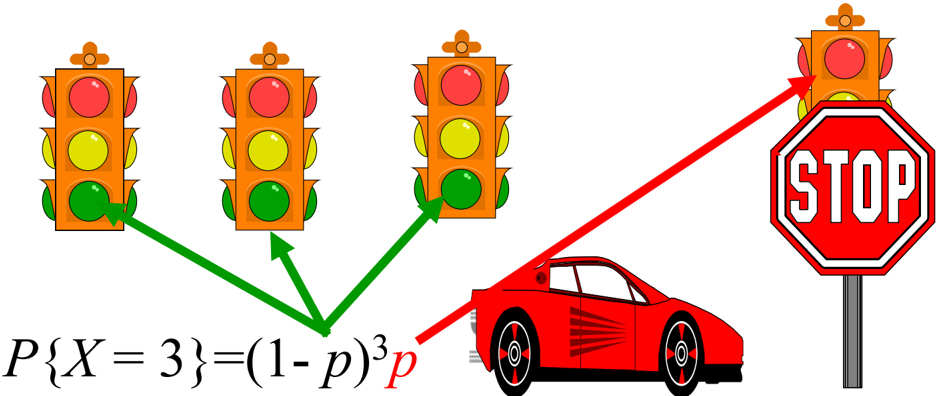
\includegraphics[width=0.6\textwidth]{figures/fig_traffic_lights.png}
    \caption{汽车经过四盏信号灯示意图，$P\{X=3\}=(1-p)^3 p$}
    \label{fig:traffic_lights}
\end{figure}

\textbf{解}：以 $p$ 表示每盏信号灯禁止汽车通过的概率，则 $p=\frac{1}{2}$。

$X$ 的取值为 $0,1,2,3,4$。
\begin{itemize}[leftmargin=2em]
    \item $\{X=0\}$：第1盏灯禁止，$P\{X=0\}=p$；
    \item $\{X=1\}$：第1盏允许，第2盏禁止，$P\{X=1\}=(1-p)p$；
    \item $\{X=2\}$：前2盏允许，第3盏禁止，$P\{X=2\}=(1-p)^2 p$；
    \item $\{X=3\}$：前3盏允许，第4盏禁止，$P\{X=3\}=(1-p)^3 p$；
    \item $\{X=4\}$：4盏全允许，$P\{X=4\}=(1-p)^4$。
\end{itemize}

一般地，可写成
\[
P\{X=k\} = (1-p)^k p, \quad k=0,1,2,3; \qquad P\{X=4\}=(1-p)^4.
\]

以 $p=\frac{1}{2}$ 代入得：

\begin{table}[htbp]
\centering
\begin{tabular}{@{}cccccc@{}}
\toprule
$X$ & 0 & 1 & 2 & 3 & 4 \\
\midrule
$P$ & 0.5 & 0.25 & 0.125 & 0.0625 & 0.0625 \\
\bottomrule
\end{tabular}
\end{table}

\subsection{一些常用的离散型随机变量}

\subsubsection{Bernoulli分布（0--1分布）}

\begin{definition}[Bernoulli分布]
如果随机变量 $X$ 的分布律为
\[
P\{X=1\}=p, \quad P\{X=0\}=1-p=q,
\]
即
\[
P\{X=k\}=p^k q^{1-k}, \quad k=0,1,
\]
则称随机变量 $X$ 服从参数为 $p$ 的\textbf{Bernoulli分布}（或\textbf{0--1分布}），记为
\[
\boxed{X \sim B(1,p)}.
\]
\end{definition}

\textbf{概率背景}：进行一次Bernoulli试验，设 $P(A)=p$，$P(\bar{A})=1-p=q$。令 $X$ 表示在这次Bernoulli试验中事件 $A$ 发生的次数，则 $X \sim B(1,p)$。

\begin{example}[产品抽样]
在15件产品中有4件次品，11件正品。从中取出1件，令 $X$ 表示取出的一件产品中的次品数，则 $X$ 的取值为0或1，且
\[
P\{X=0\} = \frac{11}{15}, \quad P\{X=1\} = \frac{4}{15},
\]
即 $X \sim B\left(1,\dfrac{4}{15}\right)$。
\end{example}

\subsubsection{二项分布}

\begin{definition}[二项分布]
如果随机变量 $X$ 的分布律为
\[
\boxed{P\{X=k\} = \dbinom{n}{k} p^k (1-p)^{n-k}, \quad k=0,1,2,\dots,n},
\]
则称随机变量 $X$ 服从参数为 $(n,p)$ 的\textbf{二项分布}，记作
\[
\boxed{X \sim B(n,p)}.
\]
\end{definition}

\begin{note}
当 $n=1$ 时，$X \sim B(1,p)$，此时退化为Bernoulli分布。这说明Bernoulli分布是二项分布的一个特例。
\end{note}

\textbf{概率背景}：进行 $n$ 重Bernoulli试验，设在每次试验中 $P(A)=p$，$P(\bar{A})=1-p=q$。令 $X$ 表示在这 $n$ 重Bernoulli试验中事件 $A$ 发生的次数，则 $X \sim B(n,p)$。

\begin{example}[产品次品率]
一大批产品的次品率为 $0.05$，现从中取出10件。设 $X$ 表示10件产品中的次品数，则 $X \sim B(10,0.05)$。试求：
\begin{itemize}[leftmargin=2em]
    \item $B = \{\text{恰有4件次品}\}$；
    \item $C = \{\text{至少有2件次品}\}$；
    \item $D = \{\text{没有次品}\}$。
\end{itemize}
\end{example}

\textbf{解}：
\begin{align*}
P(B) &= P\{X=4\} = \dbinom{10}{4} \times 0.05^4 \times 0.95^6 \approx 9.648 \times 10^{-4}, \\[0.5em]
P(C) &= P\{X \geq 2\} = 1 - P\{X=0\} - P\{X=1\} \\
&= 1 - \dbinom{10}{0}0.05^0 0.95^{10} - \dbinom{10}{1}0.05^1 0.95^9 \approx \boxed{0.0861}, \\[0.5em]
P(D) &= P\{X=0\} = 0.95^{10} \approx \boxed{0.5987}.
\end{align*}

\begin{example}[猜测答题]
考卷上有5道选择题，每道题有4个可能答案，其中只有一个答案是正确的。靠猜测至少能答对4道题的概率是多少？
\end{example}

\textbf{解}：每答一道题相当于做一次Bernoulli试验，$A=\{\text{答对一道题}\}$，则 $P(A)=\frac{1}{4}$。答5道题相当于做5重Bernoulli试验。

设 $X$ 表示该学生靠猜能答对的题数，则 $X \sim B\left(5,\dfrac{1}{4}\right)$。

\[
P\{\text{至少能答对4道题}\} = P\{X \geq 4\} = P\{X=4\} + P\{X=5\} = \dbinom{5}{4}\left(\frac{1}{4}\right)^4\frac{3}{4} + \left(\frac{1}{4}\right)^5 = \boxed{\frac{1}{64}}.
\]

\begin{example}[设备维修问题]
设有80台同类型的设备，各台工作是相互独立的，发生故障的概率都是 $0.01$，且一台设备的故障能由一个人处理。考虑两种配备维修工人的方法：
\begin{enumerate}[label=(\arabic*),leftmargin=2em]
    \item 由4人维护，每人负责20台；
    \item 由3人共同维护80台。
\end{enumerate}
试比较这两种方法在设备发生故障时不能及时维修的概率的大小。
\end{example}

\textbf{解}：

\textbf{按第一种方法}。以 $X$ 记第1人负责的20台中同一时刻发生故障的台数，则 $X \sim B(20,0.01)$。令事件 $A_i$ 表示第 $i$ 人负责的设备中发生故障不能及时维修（即该人负责的20台中至少有2台同时故障），则80台中发生故障而不能及时维修的概率为
\[
P(A_1 \cup A_2 \cup A_3 \cup A_4) \geq P(A_1) = P\{X \geq 2\} = 1 - \sum_{k=0}^{1}\dbinom{20}{k}0.01^k 0.99^{20-k} \approx 0.0169.
\]

\textbf{按第二种方法}。以 $Y$ 记80台中同一时刻发生故障的台数，则 $Y \sim B(80,0.01)$。故80台中发生故障而不能及时维修的概率为
\[
P\{Y \geq 4\} = 1 - P\{Y \leq 3\} = 1 - \sum_{k=0}^{3}\dbinom{80}{k}0.01^k 0.99^{80-k} \approx \boxed{0.0087}.
\]

\begin{note}
第二种方法中发生故障而不能及时维修的概率小，且维修工人减少一人。运用概率论讨论国民经济问题，可以有效地使用人力、物力资源。
\end{note}

\begin{example}[射击次数问题]
对同一目标进行射击，设每次射击的命中率均为 $0.23$，问至少需进行多少次射击，才能使至少命中一次目标的概率不少于 $0.95$？
\end{example}

\textbf{解}：设需进行 $n$ 次射击，进行 $n$ 次射击可看成是 $n$ 重Bernoulli试验。令 $A=\{\text{命中目标}\}$，则 $P(A)=0.23$。以 $X$ 记 $n$ 次射击中的命中次数，则 $X \sim B(n,0.23)$。

\[
P\{X \geq 1\} = 1 - P\{X=0\} = 1 - 0.77^n.
\]

由题意 $1 - 0.77^n \geq 0.95$，即
\[
0.77^n \leq 0.05 \quad\Longrightarrow\quad n \geq \frac{\ln 0.05}{\ln 0.77} \approx 11.46.
\]

故至少需进行 $\boxed{12}$ 次射击。

\subsubsection{二项分布的分布形态}

\begin{property}[二项分布的单调性]
若 $X \sim B(n,p)$，则
\[
\frac{P\{X=k\}}{P\{X=k-1\}} = \frac{(n-k+1)p}{kq} = 1 + \frac{(n+1)p - k}{kq}.
\]
因此
\[
\frac{P\{X=k\}}{P\{X=k-1\}} \begin{cases} >1, & k<(n+1)p, \\ =1, & k=(n+1)p, \\ <1, & k>(n+1)p. \end{cases}
\]
\end{property}

\begin{note}
由此可知，二项分布的分布 $P\{X=k\}$ 先是随着 $k$ 的增大而增大，达到其最大值后再随着 $k$ 的增大而减少。
\end{note}

\begin{figure}[htbp]
    \centering
    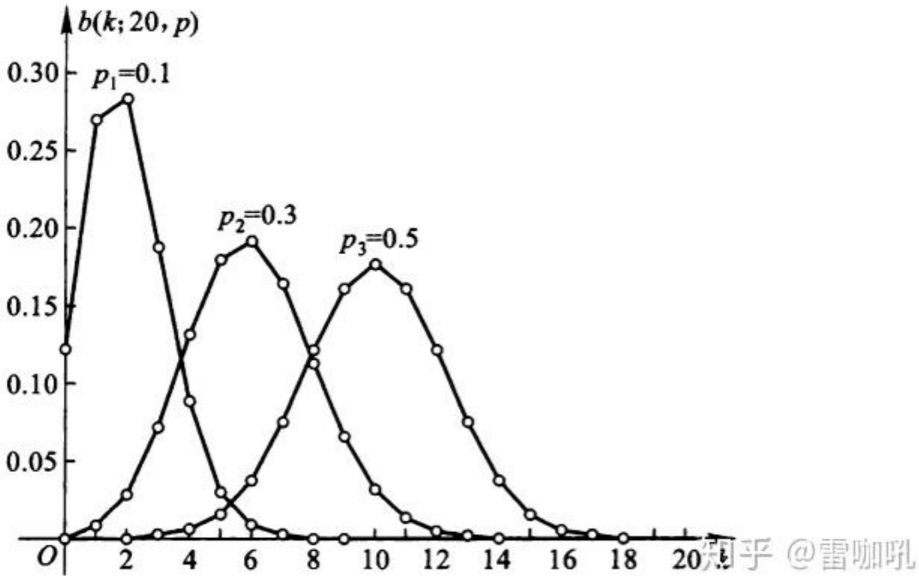
\includegraphics[width=0.6\textwidth]{figures/fig_binomial_shape.png}
    \caption{二项分布分布形态示意图（$n=20$, $p=0.1,0.3,0.5$ 三条曲线）}
    \label{fig:binomial_shape}
\end{figure}

\begin{definition}[最大可能次数]
使得 $P\{X=k\}$ 达到其最大值的 $k_0$ 称为该二项分布的\textbf{最大可能次数}。
\begin{itemize}[leftmargin=2em]
    \item 若 $(n+1)p$ 是整数，则 $k_0 = (n+1)p$ 或 $(n+1)p-1$；
    \item 若 $(n+1)p$ 不是整数，则 $k_0 = \lfloor (n+1)p \rfloor$（取整数部分）。
\end{itemize}
\end{definition}

\begin{example}[最可能命中次数]
对同一目标进行400次独立射击，设每次射击时的命中率均为 $0.02$，试求400次射击最可能命中几次？
\end{example}

\textbf{解}：令 $X$ 表示400次射击命中目标的次数，则 $X \sim B(400,0.02)$。

由于 $(400+1) \times 0.02 = 8.02$ 不是整数，因此最可能射击的命中次数为
\[
\boxed{k_0 = \lfloor 8.02 \rfloor = 8}.
\]

\subsubsection{Poisson分布}

\begin{definition}[Poisson分布]
如果随机变量 $X$ 的分布律为
\[
\boxed{P\{X=k\} = \frac{\lambda^k}{k!}e^{-\lambda}, \quad k=0,1,2,\dots}
\]
（其中 $\lambda > 0$ 为常数），则称随机变量 $X$ 服从参数为 $\lambda$ 的\textbf{Poisson分布}（泊松分布），记为
\[
\boxed{X \sim P(\lambda)}.
\]
\end{definition}

\begin{figure}[htbp]
    \centering
    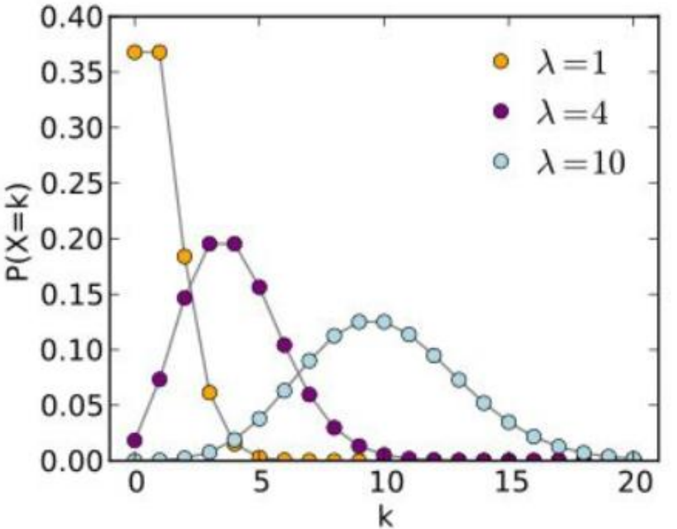
\includegraphics[width=0.6\textwidth]{figures/fig_poisson_dist.png}
    \caption{Poisson分布示意图（$\lambda=1,4,10$ 三条曲线对比）}
    \label{fig:poisson_dist}
\end{figure}

\textbf{Poisson分布的应用}：
\begin{itemize}[leftmargin=2em]
    \item Poisson分布是概率论中重要的分布之一；
    \item 自然界及工程技术中的许多随机指标都服从Poisson分布；
    \item 它多出现在当 $X$ 表示在一定的时间或空间内出现的事件个数这种场合。
\end{itemize}

例如，电话总机在某一时间间隔内收到的呼叫次数，放射物在某一时间间隔内发射的粒子数，容器在某一时间间隔内产生的细菌数，某一时间间隔内来到某服务台要求服务的人数等，在一定条件下，都是服从Poisson分布的。

\begin{example}[例12：求Poisson分布的参数]
设随机变量 $X$ 服从参数为 $\lambda$ 的Poisson分布，且已知 $P\{X=1\}=P\{X=2\}$，试求 $P\{X=4\}$。
\end{example}

\textbf{解}：随机变量 $X$ 的分布律为
\[
P\{X=k\} = \frac{\lambda^k}{k!}e^{-\lambda}, \quad k=0,1,2,\dots
\]
由 $P\{X=1\}=P\{X=2\}$，有
\[
\lambda e^{-\lambda} = \frac{\lambda^2}{2}e^{-\lambda} \quad\Longrightarrow\quad \lambda^2 - 2\lambda = 0.
\]
解得 $\lambda=2$（$\lambda=0$ 不合题意，忽略）。于是
\[
\boxed{P\{X=4\} = \frac{2^4}{4!}e^{-2} = \frac{2}{3}e^{-2} \approx 0.09022}.
\]

\begin{example}[例13：Bayes公式与Poisson分布]
设一个人在一年中得感冒次数服从参数 $\lambda=5$ 的Poisson分布。现有一种预防感冒的药，对 $30\%$ 的人可将参数降为 $\lambda=1$（疗效显著）；对另外 $45\%$ 的人可将参数降为 $\lambda=4$（疗效一般）；对其余 $25\%$ 的人则无效。现某人服用此药一年，其间得了3次感冒，求此药对他``疗效显著''的概率。
\end{example}

\textbf{解}：设 $B=\{\text{此人在一年中得3次感冒}\}$，$A_1=\{\text{疗效显著}\}$，$A_2=\{\text{疗效一般}\}$，$A_3=\{\text{该药无效}\}$。

由Bayes公式得
\[
P(A_1 \mid B) = \frac{P(A_1)P(B \mid A_1)}{P(A_1)P(B \mid A_1)+P(A_2)P(B \mid A_2)+P(A_3)P(B \mid A_3)}
\]
其中
\[
P(B \mid A_1) = \frac{1^3}{3!}e^{-1}, \quad P(B \mid A_2) = \frac{4^3}{3!}e^{-4}, \quad P(B \mid A_3) = \frac{5^3}{3!}e^{-5}.
\]
代入得
\[
\boxed{P(A_1 \mid B) \approx 0.1301}.
\]

\begin{theorem}[Poisson定理]
设随机变量 $X_n\;(n=1,2,\dots)$ 服从二项分布，其分布律为
\[
P\{X_n=k\} = \dbinom{n}{k}p_n^k(1-p_n)^{n-k}, \quad k=0,1,\dots,n.
\]
设 $np_n = \lambda > 0$ 为常数，则
\[
\boxed{\lim_{n\to\infty} P\{X_n=k\} = \lim_{n\to\infty}\dbinom{n}{k}p_n^k(1-p_n)^{n-k} = \frac{\lambda^k}{k!}e^{-\lambda}}.
\]
\end{theorem}

\begin{proof}
由 $p_n = \lambda/n$，有
\[
\dbinom{n}{k}p_n^k(1-p_n)^{n-k} = \frac{n(n-1)\cdots(n-k+1)}{k!}\left(\frac{\lambda}{n}\right)^k\left(1-\frac{\lambda}{n}\right)^{n-k}.
\]
注意到
\[
\lim_{n\to\infty}\left(1-\frac{1}{n}\right)\left(1-\frac{2}{n}\right)\cdots\left(1-\frac{k-1}{n}\right)=1, \quad \lim_{n\to\infty}\left(1-\frac{\lambda}{n}\right)^n = e^{-\lambda}, \quad \lim_{n\to\infty}\left(1-\frac{\lambda}{n}\right)^{-k}=1.
\]
所以
\[
\lim_{n\to\infty}\dbinom{n}{k}p_n^k(1-p_n)^{n-k} = \frac{\lambda^k}{k!}e^{-\lambda}.
\]
\end{proof}

\begin{note}
若随机变量 $X \sim B(n,p)$，则当 $n$ 比较大、$p$ 比较小时，令 $\lambda=np$，有
\[
P\{X=k\} = \dbinom{n}{k}p^k(1-p)^{n-k} \approx \frac{\lambda^k}{k!}e^{-\lambda}.
\]
\end{note}

\begin{example}[例14：Poisson近似计算]
设每次射击命中目标的概率为 $0.012$，现射击 $600$ 次，求至少命中 $3$ 次目标的概率（用Poisson分布近似计算）。
\end{example}

\textbf{解}：设 $B=\{600\text{次射击至少命中3次目标}\}$。进行 $600$ 次射击可看作是 $600$ 重Bernoulli试验。令 $X$ 表示 $600$ 次射击命中目标的次数，则 $X \sim B(600,0.012)$。

用Poisson分布近似计算，取 $\lambda = 600 \times 0.012 = 7.2$。
\[
P(B) = P\{X \geq 3\} = 1 - P\{X < 3\} = 1 - P\{X=0\} - P\{X=1\} - P\{X=2\}
\]
\[
\approx 1 - e^{-7.2} - 7.2e^{-7.2} - \frac{7.2^2}{2}e^{-7.2} \approx \boxed{0.9745}.
\]

\subsubsection{几何分布}

\begin{definition}[几何分布]
若随机变量 $X$ 的分布律为
\[
\boxed{P\{X=k\} = q^{k-1}p, \quad k=1,2,\dots}
\]
（其中 $p \geq 0,\; q \geq 0,\; p+q=1$），则称随机变量 $X$ 服从参数为 $p$ 的\textbf{几何分布}。
\end{definition}

\textbf{概率背景}：在Bernoulli试验中，$P(A)=p$，$P(\bar{A})=q=1-p$。试验进行到 $A$ 首次出现为止，令 $X$ 表示所需试验次数，则 $X$ 服从参数为 $p$ 的几何分布。

事件 $\{X=k\}$ 表示``前 $k-1$ 次试验中 $A$ 不出现，第 $k$ 次试验中 $A$ 出现''，故 $P\{X=k\}=q^{k-1}p$。

\begin{example}[例15：射击次数问题]
对同一目标进行射击，设每次射击时的命中率为 $0.64$，射击进行到击中目标时为止。令 $X$ 表示所需射击次数，试求 $X$ 的分布律，并求至少进行 $2$ 次射击才能击中目标的概率。
\end{example}

\textbf{解}：$X$ 的取值为 $1,2,\dots,n,\dots$，$X$ 服从参数为 $p=0.64$ 的几何分布，故 $X$ 的分布律为
\[
P\{X=n\} = 0.36^{n-1} \cdot 0.64, \quad n=1,2,\dots
\]
至少进行2次射击才能击中目标的概率为
\[
P\{X \geq 2\} = \sum_{n=2}^{\infty} 0.36^{n-1} \cdot 0.64 = 0.64 \times \frac{0.36}{1-0.36} = \boxed{0.36}.
\]

\subsubsection{超几何分布}

\begin{definition}[超几何分布]
如果随机变量 $X$ 的分布律为
\[
\boxed{P\{X=k\} = \frac{\dbinom{M}{k}\dbinom{N-M}{n-k}}{\dbinom{N}{n}}, \quad k=0,1,\dots,\min(M,n)}
\]
其中 $N,M,n$ 均为自然数，则称随机变量 $X$ 服从参数为 $(N,M,n)$ 的\textbf{超几何分布}。
\end{definition}

\textbf{概率背景}：一批产品有 $N$ 件，其中有 $M$ 件次品，其余 $N-M$ 件为正品。现从中取出 $n$ 件，令 $X$ 表示取出 $n$ 件产品中的次品数，则 $X$ 的分布律为上式，即 $X$ 服从参数为 $(N,M,n)$ 的超几何分布。

\begin{note}
\begin{itemize}[leftmargin=2em]
    \item 这个分布在涉及抽样的问题中常用，特别当 $N$ 不大时。因为通常在抽样时多是``无放回的''，这就与同时抽出的效果一样。
    \item 如果是``有放回的抽样''，结果是二项分布。
    \item 若 $n/N$ 很小，则放回与不放回差别不大。在这种情况下超几何分布与二项分布很接近。
    \item 确切地说，若 $X$ 服从超几何分布，则当 $n$ 固定、$M/N$ 固定、$N \to \infty$ 时，$X$ 近似地服从二项分布。
\end{itemize}
\end{note}

% ==================== §3 随机变量的分布函数 ====================
\section{随机变量的分布函数}

\subsection{分布函数的定义及其性质}

\begin{definition}[分布函数]
设 $X$ 是一个随机变量，$x$ 是任意实数，函数
\[
\boxed{F(x) = P\{X \leq x\}}
\]
称为 $X$ 的\textbf{分布函数}。
\end{definition}

\begin{figure}[htbp]
    \centering
    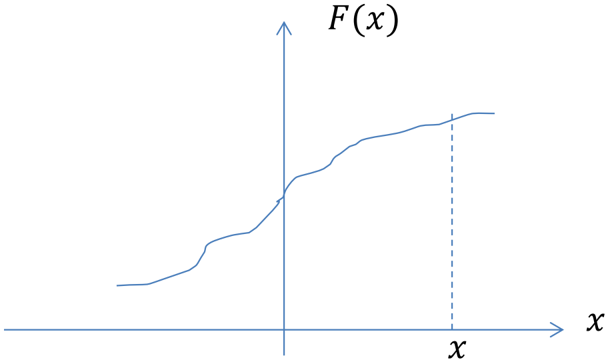
\includegraphics[width=0.5\textwidth]{figures/fig_distribution_func.png}
    \caption{分布函数 $F(x)$ 示意图（单调不减、右连续）}
    \label{fig:distribution_func}
\end{figure}

\begin{note}
$F(x)$ 是 $x$ 的实值单调不减函数，且 $x \in (-\infty,+\infty)$ 时 $F(x) \in [0,1]$。
\end{note}

\begin{property}[分布函数的性质]
\begin{enumerate}[label=(\arabic*),leftmargin=2em]
    \item \textbf{单调不减}：若 $x_1 < x_2$，则 $F(x_1) \leq F(x_2)$。
    
    \textit{证}：由于 $x_1 < x_2$，有 $\{X \leq x_1\} \subset \{X \leq x_2\}$，故
    \[
    F(x_1) = P\{X \leq x_1\} \leq P\{X \leq x_2\} = F(x_2).
    \]
    
    \item \textbf{有界性}：$0 \leq F(x) \leq 1$，且
    \[
    F(-\infty) = \lim_{x\to-\infty}F(x) = 0, \qquad F(+\infty) = \lim_{x\to+\infty}F(x) = 1.
    \]
    
    \item \textbf{右连续性}：$F(x+0) = F(x)$，即 $F(x)$ 是右连续的。
\end{enumerate}
\end{property}

\textbf{应用：用分布函数计算事件的概率}

对任意实数 $x_1 \leq x_2$，有
\[
P\{x_1 < X \leq x_2\} = P\{X \leq x_2\} - P\{X \leq x_1\} = F(x_2) - F(x_1).
\]

\begin{figure}[htbp]
    \centering
    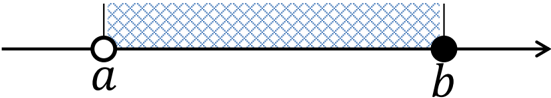
\includegraphics[width=0.5\textwidth]{figures/fig_interval_prob.png}
    \caption{区间概率示意图（数轴上 $(a,b]$ 的表示）}
    \label{fig:interval_prob}
\end{figure}

更一般地：
\begin{align*}
P\{X < a\} &= \lim_{x\to a^-}F(x) = F(a-0), \\
P\{X = a\} &= P\{X \leq a\} - P\{X < a\} = F(a) - F(a-0), \\
P\{a \leq X \leq b\} &= F(b) - F(a-0), \\
P\{a < X < b\} &= F(b-0) - F(a), \\
P\{a \leq X < b\} &= F(b-0) - F(a-0), \\
P\{X > b\} &= 1 - F(b), \\
P\{X \geq b\} &= 1 - F(b-0).
\end{align*}

\begin{example}[例1：分段分布函数]
设随机变量 $X$ 的分布函数为
\[
F(x) = \begin{cases}
0, & x < 0, \\[0.3em]
\dfrac{x}{2}, & 0 \leq x < 1, \\[0.5em]
\dfrac{2}{3}, & 1 \leq x < 2, \\[0.5em]
\dfrac{11}{12}, & 2 \leq x < 3, \\[0.5em]
1, & 3 \leq x.
\end{cases}
\]
求 $P\{X \leq 3\}$，$P\{X < 3\}$，$P\{X=1\}$，$P\{X > \frac{1}{2}\}$，$P\{2 < X < 4\}$，$P\{1 \leq X < 3\}$。
\end{example}

\begin{figure}[htbp]
    \centering
    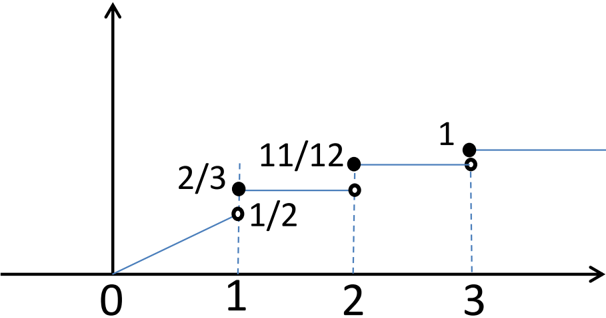
\includegraphics[width=0.5\textwidth]{figures/fig_piecewise_df.png}
    \caption{分段分布函数的阶梯示意图}
    \label{fig:piecewise_df}
\end{figure}

\textbf{解}：
\begin{align*}
P\{X \leq 3\} &= F(3) = 1, \\
P\{X < 3\} &= F(3-0) = \frac{11}{12}, \\
P\{X=1\} &= F(1) - F(1-0) = \frac{2}{3} - \frac{1}{2} = \frac{1}{6}, \\
P\{X > \tfrac{1}{2}\} &= 1 - F(\tfrac{1}{2}) = 1 - \frac{1}{4} = \frac{3}{4}, \\
P\{2 < X < 4\} &= F(4-0) - F(2) = 1 - \frac{11}{12} = \frac{1}{12}, \\
P\{1 \leq X < 3\} &= F(3-0) - F(1-0) = \frac{11}{12} - \frac{1}{2} = \frac{5}{12}.
\end{align*}

\begin{example}[例2：确定分布函数中的常数]
设随机变量 $X$ 的分布函数为
\[
F(x) = A + B\arctan x, \quad -\infty < x < \infty.
\]
试求常数 $A,B$。
\end{example}

\textbf{解}：由分布函数的性质，
\[
\lim_{x\to-\infty}F(x) = A - \frac{\pi}{2}B = 0, \qquad \lim_{x\to+\infty}F(x) = A + \frac{\pi}{2}B = 1.
\]
解得
\[
\boxed{A = \frac{1}{2}, \quad B = \frac{1}{\pi}}.
\]

\begin{example}[例3：右连续性确定常数]
设随机变量 $X$ 的分布函数为
\[
F(x) = \begin{cases}
0, & x < 0, \\[0.3em]
A\sin x, & 0 \leq x \leq \dfrac{\pi}{2}, \\[0.5em]
1, & x > \dfrac{\pi}{2}.
\end{cases}
\]
试确定 $A$。
\end{example}

\textbf{解}：由分布函数的右连续性，
\[
F\left(\frac{\pi}{2}+0\right) = F\left(\frac{\pi}{2}\right) = A\sin\frac{\pi}{2} = A = 1.
\]
故 $\boxed{A=1}$。

\subsection{离散型随机变量的分布函数}

\begin{example}[例4：由分布律求分布函数]
设随机变量 $X$ 的分布律为
\begin{table}[htbp]
\centering
\begin{tabular}{@{}cccc@{}}
\toprule
$X$ & $-1$ & $2$ & $3$ \\
\midrule
$P$ & $\dfrac{1}{4}$ & $\dfrac{1}{2}$ & $\dfrac{1}{4}$ \\
\bottomrule
\end{tabular}
\end{table}
求 $X$ 的分布函数。
\end{example}

\textbf{解}：
\begin{itemize}[leftmargin=2em]
    \item 当 $x < -1$ 时，$\{X \leq x\} = \varnothing$，故 $F(x)=0$；
    \item 当 $-1 \leq x < 2$ 时，$F(x)=P\{X \leq x\}=P\{X=-1\}=\dfrac{1}{4}$；
    \item 当 $2 \leq x < 3$ 时，$F(x)=P\{X=-1\}+P\{X=2\}=\dfrac{1}{4}+\dfrac{1}{2}=\dfrac{3}{4}$；
    \item 当 $x \geq 3$ 时，$F(x)=1$。
\end{itemize}

因此
\[
F(x) = \begin{cases}
0, & x < -1, \\[0.3em]
\dfrac{1}{4}, & -1 \leq x < 2, \\[0.5em]
\dfrac{3}{4}, & 2 \leq x < 3, \\[0.5em]
1, & x \geq 3.
\end{cases}
\]

\begin{figure}[htbp]
    \centering
    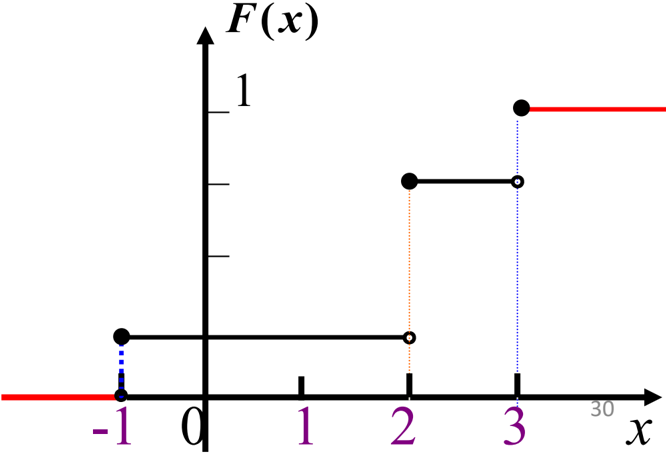
\includegraphics[width=0.5\textwidth]{figures/fig_discrete_cdf_steps.png}
    \caption{离散型分布函数阶梯图（在 $-1,2,3$ 处有跳跃）}
    \label{fig:discrete_cdf_steps}
\end{figure}

\textbf{一般地}，设离散型随机变量 $X$ 的分布律为
\[
P\{X=x_k\}=p_k, \quad k=1,2,\dots
\]
则 $X$ 的分布函数为
\[
F(x) = P(X \leq x) = \sum_{x_k \leq x} P\{X=x_k\}.
\]

\begin{note}
此函数为\textbf{阶梯函数}，且在 $X=x_k\;(k=1,2,\dots)$ 处有跳跃，其跳跃值为 $P\{X=x_k\}=p_k$。
\end{note}

\begin{example}[例5：由分布函数求分布律]
设随机变量 $X$ 的分布函数为
\[
F(x) = \begin{cases}
0, & x < 0, \\[0.3em]
\dfrac{1}{3}, & 0 \leq x < 1, \\[0.5em]
\dfrac{1}{2}, & 1 \leq x < 2, \\[0.5em]
1, & x \geq 2.
\end{cases}
\]
求 $X$ 的分布律。
\end{example}

\textbf{解}：$X$ 的可能取值为 $0,1,2$。利用 $P\{X=a\}=F(a)-F(a-0)$，
\[
P\{X=0\} = \frac{1}{3}, \quad P\{X=1\} = \frac{1}{2}-\frac{1}{3} = \frac{1}{6}, \quad P\{X=2\} = 1-\frac{1}{2} = \frac{1}{2}.
\]

\begin{example}[例6：靶子问题]
一个靶子是半径为 $2$ 米的圆盘，设击中靶上任一同心圆盘上的点的概率与该圆盘的面积成正比，并设射击都能中靶。以 $X$ 表示弹着点与圆心的距离，试求随机变量 $X$ 的分布函数。
\end{example}

\begin{figure}[htbp]
    \centering
    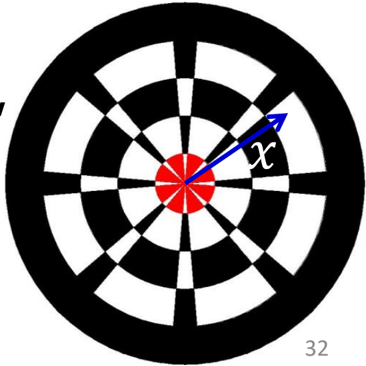
\includegraphics[width=0.5\textwidth]{figures/fig_target.png}
    \caption{靶子示意图（圆盘、弹着点距离 $x$）}
    \label{fig:target}
\end{figure}

\textbf{解}：$X \geq 0$。由于 $F(x)=P\{X \leq x\}$：
\begin{enumerate}[label=(\arabic*),leftmargin=2em]
    \item 若 $x < 0$，则 $\{X \leq x\}$ 是不可能事件，$F(x)=0$；
    \item 若 $0 \leq x \leq 2$，则 $F(x)=P\{0 \leq X \leq x\} = kx^2$。由 $P\{0 \leq X \leq 2\}=1$ 得 $k=\dfrac{1}{4}$，故 $F(x)=\dfrac{x^2}{4}$；
    \item 若 $x \geq 2$，则 $\{X \leq x\}$ 是必然事件，$F(x)=1$。
\end{enumerate}

于是分布函数为
\[
F(x) = \begin{cases}
0, & x < 0, \\[0.3em]
\dfrac{x^2}{4}, & 0 \leq x < 2, \\[0.5em]
1, & x \geq 2.
\end{cases}
\]

\begin{note}
不同的随机变量，它们的分布函数不一定相同。例如抛均匀硬币，令
\[
X_1 = \begin{cases} 1, & \text{正面}, \\ -1, & \text{反面}, \end{cases} \qquad
X_2 = \begin{cases} 1, & \text{反面}, \\ -1, & \text{正面}. \end{cases}
\]
$X_1$ 与 $X_2$ 在样本空间上对应法则不同，是两个不同的随机变量，但它们有相同的分布函数
\[
F(x) = \begin{cases} 0, & x < -1, \\[0.3em] \dfrac{1}{2}, & -1 \leq x < 1, \\[0.5em] 1, & x \geq 1. \end{cases}
\]
\end{note}

% ==================== §4 连续型随机变量及其概率密度 ====================
\section{连续型随机变量及其概率密度}

\subsection{概率密度函数的导出}

从离散到连续——将连续情形看成越来越小、离散单元的极限。

一个好的``随机数生成器''赋予 $0$ 到 $1$ 之间任何一个数字以等概率。问题在于每一个数的概率为零，而它们的概率之和必须为 $1$。

近似：考虑随机数生成器仅给出一个有限位精度的数字。当有一位小数精度时，有 $10$ 个简单事件；当用两个小数精度时，有 $100$ 个简单事件。

新型直方图：用\textbf{面积}（而不是高度）来表示概率。

\textbf{概率密度函数}：假设简单事件可以用实数 $x$ 为指标，$a \leq x \leq b$。一个函数 $f(x)$ 若满足
\begin{enumerate}[label=(\arabic*),leftmargin=2em]
    \item 对所有 $a \leq x \leq b$，有 $f(x) \geq 0$；
    \item $\displaystyle\int_a^b f(x)\,dx = 1$，
\end{enumerate}
则称其为\textbf{概率密度函数}。

\subsection{连续型随机变量的概念与性质}

\begin{definition}[连续型随机变量]
如果对于随机变量 $X$ 的分布函数 $F(x)$，存在非负实函数 $f(x)$，使得对于任意实数 $x$，有
\[
\boxed{F(x) = \int_{-\infty}^{x} f(t)\,dt},
\]
则称 $X$ 为\textbf{连续型随机变量}，其中 $f(x)$ 称为 $X$ 的\textbf{概率密度函数}（简称概率密度或密度函数）。
\end{definition}

\begin{note}
$f(x)$ 不一定连续，但 $F(x)$ 一定连续。
\end{note}

\begin{figure}[htbp]
    \centering
    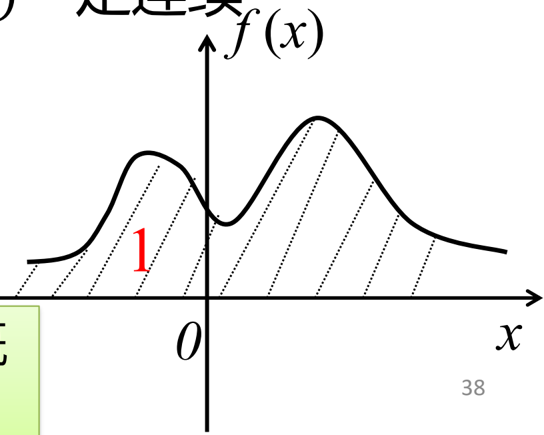
\includegraphics[width=0.5\textwidth]{figures/fig_pdf.png}
    \caption{概率密度函数 $f(x)$ 示意图（曲线下面积为 $1$）}
    \label{fig:pdf}
\end{figure}

\begin{property}[概率密度的性质]
\begin{enumerate}[label=(\arabic*),leftmargin=2em]
    \item \textbf{非负性}：$f(x) \geq 0$；
    \item \textbf{归一化}：$\displaystyle\int_{-\infty}^{+\infty} f(x)\,dx = 1$。
\end{enumerate}
这两条性质是判定 $f(x)$ 是否为概率密度函数的充要条件。
\end{property}

\begin{property}[概率的计算]
对任意 $x_1 < x_2$，
\[
P\{x_1 < X \leq x_2\} = F(x_2) - F(x_1) = \int_{x_1}^{x_2} f(x)\,dx.
\]
\end{property}

\begin{figure}[htbp]
    \centering
    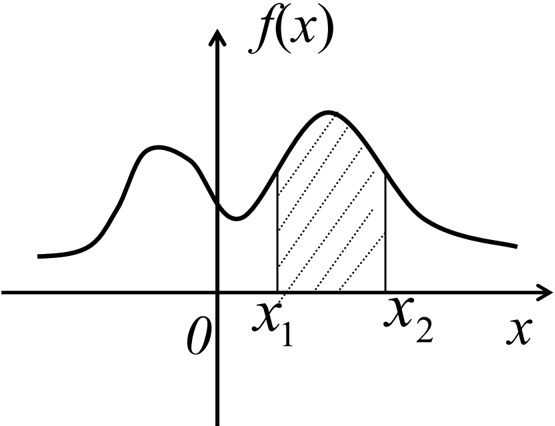
\includegraphics[width=0.5\textwidth]{figures/fig_pdf_interval.png}
    \caption{区间概率示意图（$f(x)$ 在 $[x_1,x_2]$ 上的面积）}
    \label{fig:pdf_interval}
\end{figure}

\begin{property}
若 $f(x)$ 在点 $x$ 处连续，则
\[
F'(x) = f(x).
\]
\end{property}

\textbf{对 $f(x)$ 的进一步理解}：
\begin{enumerate}[label=(\arabic*),leftmargin=2em]
    \item 若 $x$ 是 $f(x)$ 的连续点，则
    \[
    \lim_{\Delta x \to 0} \frac{P\{x < X \leq x+\Delta x\}}{\Delta x} = \lim_{\Delta x \to 0} \frac{\int_x^{x+\Delta x} f(t)\,dt}{\Delta x} = f(x).
    \]
    类比：概率密度 $\leftrightarrow$ 概率；物质密度 $\leftrightarrow$ 物质质量；速度 $\leftrightarrow$ 距离。
    
    \item 若不计高阶无穷小，有
    \[
    P\{x < X \leq x+\Delta x\} \approx f(x)\Delta x.
    \]
    它表示 $X$ 取值于 $(x,x+\Delta x]$ 的概率近似等于 $f(x)\Delta x$。$f(x)\Delta x$ 在连续型随机变量理论中所起的作用与 $P\{X=x_k\}=p_k$ 在离散型随机变量理论中所起的作用类似。
    
    \item 连续型随机变量取任一指定值的概率为 $0$，即
    \[
    P\{X=a\} = 0, \quad a \text{ 为任一指定值}.
    \]
    \textit{证}：
    \[
    0 \leq P\{X=a\} \leq \lim_{\epsilon\to 0}[F(a)-F(a-\epsilon)] = 0.
    \]
    
    由此得，对连续型 $X$，
    \[
    P\{a \leq X \leq b\} = P\{a < X \leq b\} = P\{a \leq X < b\} = P\{a < X < b\}.
    \]
    这与离散型有很大差别。
    
    注意：$P\{X=a\}=0$ 并不意味着 $\{X=a\}$ 是不可能事件；$P(B)=1$ 也并不意味着 $B=\Omega$。
    
    \item $f(x)$ 在某点 $a$ 处的高度，不反映 $X$ 取值的概率，只意味着 $X$ 取 $a$ 附近的值的概率的大小。
\end{enumerate}

\begin{figure}[htbp]
    \centering
    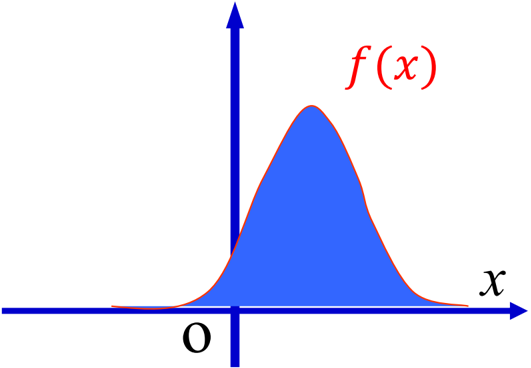
\includegraphics[width=0.5\textwidth]{figures/fig_pdf_height.png}
    \caption{概率密度在某点高度意义的示意图}
    \label{fig:pdf_height}
\end{figure}

\begin{example}[例1：分子离开细胞的概率密度]
若一个分子离开细胞非常快，概率密度函数可能为
\[
f(t) = \begin{cases} 10e^{-10t}, & t \geq 0, \\ 0, & \text{otherwise}. \end{cases}
\]
$t=0$ 时概率密度函数值较大，表示在 $t=0$ 附近分子更趋向于离开细胞。
\end{example}

\begin{figure}[htbp]
    \centering
    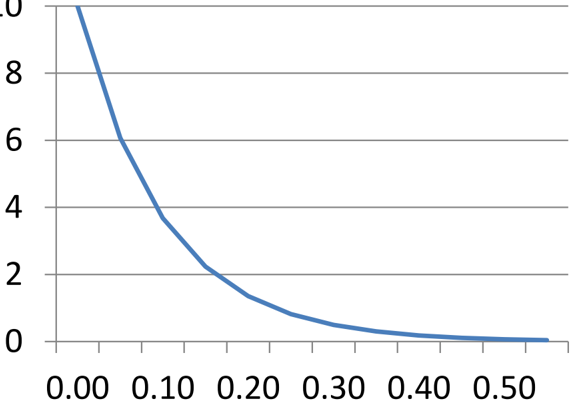
\includegraphics[width=0.5\textwidth]{figures/fig_exponential_decay.png}
    \caption{指数衰减曲线 $f(t)=10e^{-10t}$}
    \label{fig:exponential_decay}
\end{figure}

\textbf{解}：一个分子在时刻 $0.1$ 和 $0.2$ 之间离开的概率为
\[
P\{0.1 \leq t \leq 0.2\} = \int_{0.1}^{0.2} 10e^{-10t}\,dt = -e^{-10t}\Big|_{0.1}^{0.2} \approx 0.233.
\]

\begin{note}[与离散情形的不同]
\begin{enumerate}[leftmargin=2em]
    \item 对于连续型随机变量，不关心在某一点的概率取值，而关心在某一区间上的概率取值。
    \item 若连续型随机变量 $X$ 的概率密度为 $f(x)$，则 $X$ 在任意区间 $G$（可开、可闭、半开半闭、有限或无限）上的概率均为
    \[
    P\{X \in G\} = \int_G f(x)\,dx.
    \]
\end{enumerate}
\end{note}

\begin{example}[例2：求密度函数中的常数]
设 $X$ 是连续型随机变量，其密度函数为
\[
f(x) = \begin{cases} c(4x-2x^2), & 0 < x < 2, \\ 0, & \text{otherwise}. \end{cases}
\]
求：(1) 常数 $c$；(2) $P\{X > 1\}$；(3) $X$ 的分布函数。
\end{example}

\textbf{解}：
\begin{enumerate}[label=(\arabic*),leftmargin=2em]
    \item 由密度函数的归一化性质，
    \[
    \int_0^2 c(4x-2x^2)\,dx = c\left[2x^2-\frac{2}{3}x^3\right]_0^2 = \frac{8}{3}c = 1 \quad\Longrightarrow\quad \boxed{c=\frac{3}{8}}.
    \]
    
    \item
    \[
    P\{X > 1\} = \int_1^2 \frac{3}{8}(4x-2x^2)\,dx = \frac{3}{8}\left[2x^2-\frac{2}{3}x^3\right]_1^2 = \boxed{\frac{1}{2}}.
    \]
    
    \item 当 $x \leq 0$ 时，$F(x)=0$；当 $0 < x < 2$ 时，
    \[
    F(x) = \int_0^x \left(\frac{3t}{2}-\frac{3t^2}{4}\right)dt = \frac{3x^2}{4}-\frac{x^3}{4};
    \]
    当 $x \geq 2$ 时，$F(x)=1$。因此
    \[
    F(x) = \begin{cases}
    0, & x \leq 0, \\[0.3em]
    \dfrac{3x^2}{4}-\dfrac{x^3}{4}, & 0 < x < 2, \\[0.5em]
    1, & x \geq 2.
    \end{cases}
    \]
\end{enumerate}

\begin{example}[例3：由分布函数求密度函数]
设随机变量 $X$ 的分布函数为
\[
F(x) = \begin{cases}
0, & x \leq 0, \\[0.3em]
\dfrac{x^2}{2}, & 0 < x \leq 1, \\[0.5em]
-\dfrac{x^2}{2}+2x-1, & 1 < x < 2, \\[0.5em]
1, & 2 \leq x.
\end{cases}
\]
试求 $X$ 的密度函数 $f(x)$。
\end{example}

\textbf{解}：由于 $f(x)=F'(x)$，故
\[
f(x) = \begin{cases}
x, & 0 < x \leq 1, \\[0.3em]
2-x, & 1 < x \leq 2, \\[0.3em]
0, & \text{otherwise}.
\end{cases}
\]

\begin{example}[例4：确定分布函数中的系数]
设随机变量 $X$ 的分布函数为
\[
F(x) = \begin{cases}
A+Be^{-\frac{x^2}{2}}, & x > 0, \\[0.3em]
0, & x \leq 0.
\end{cases}
\]
试求：(1) 系数 $A,B$；(2) $X$ 的密度函数。
\end{example}

\textbf{解}：
\begin{enumerate}[label=(\arabic*),leftmargin=2em]
    \item 由分布函数的性质，
    \[
    F(+\infty) = A = 1, \qquad F(0+) = A+B = 0.
    \]
    解得
    \[
    \boxed{A=1,\quad B=-1}.
    \]
    因此
    \[
    F(x) = \begin{cases}
    1-e^{-\frac{x^2}{2}}, & x > 0, \\[0.3em]
    0, & x \leq 0.
    \end{cases}
    \]
    
    \item 设 $X$ 的密度函数为 $f(x)$，则
    \[
    f(x) = F'(x) = \begin{cases}
    xe^{-\frac{x^2}{2}}, & x > 0, \\[0.3em]
    0, & x \leq 0.
    \end{cases}
    \]
\end{enumerate}

\begin{example}[例5：电子元件寿命]
某电子元件的寿命 $X$（单位：小时）是以
\[
f(x) = \begin{cases}
\dfrac{100}{x^2}, & x > 100, \\[0.5em]
0, & x \leq 100
\end{cases}
\]
为密度函数的连续型随机变量。求 $5$ 个同类型的元件在使用的前 $150$ 小时内恰有 $2$ 个需要更换的概率。
\end{example}

\textbf{解}：设 $A=\{\text{某元件在使用的前150小时内需要更换}\}$，则
\[
P(A) = P\{X \leq 150\} = \int_{100}^{150} \frac{100}{x^2}\,dx = 100\left[-\frac{1}{x}\right]_{100}^{150} = \frac{1}{3}.
\]

检验 $5$ 个元件的使用寿命可以看作是在做一个 $5$ 重Bernoulli试验。以 $Y$ 记 $5$ 个元件中使用寿命不超过 $150$ 小时的元件数，则 $Y \sim B\left(5,\dfrac{1}{3}\right)$。

设 $B=\{5\text{个元件中恰有2个的使用寿命不超过150小时}\}$，则
\[
P(B) = P\{Y=2\} = \dbinom{5}{2}\left(\frac{1}{3}\right)^2\left(\frac{2}{3}\right)^3 = \boxed{\frac{80}{243}}.
\]

\subsection{一些常用的连续型随机变量}

\subsubsection{均匀分布}

\begin{definition}[均匀分布]
若随机变量 $X$ 的密度函数为
\[
\boxed{f(x) = \begin{cases}
\dfrac{1}{b-a}, & a \leq x \leq b, \\[0.5em]
0, & \text{otherwise},
\end{cases}}
\]
则称随机变量 $X$ 服从区间 $[a,b]$ 上的\textbf{均匀分布}，记作
\[
\boxed{X \sim U[a,b]}.
\]
\end{definition}

\begin{figure}[htbp]
    \centering
    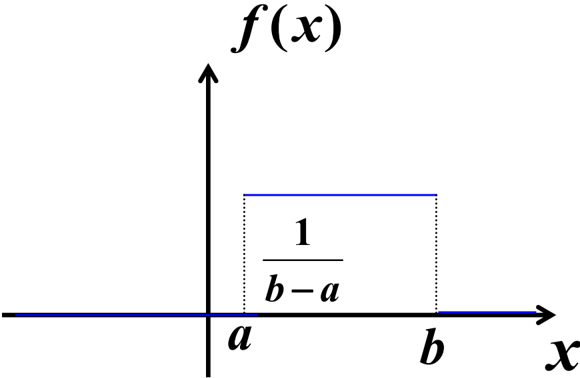
\includegraphics[width=0.5\textwidth]{figures/fig_uniform_pdf.png}
    \caption{均匀分布密度函数示意图（矩形）}
    \label{fig:uniform_pdf}
\end{figure}

\textbf{密度函数的验证}：
\begin{enumerate}[leftmargin=2em]
    \item 对任意的 $x$，有 $f(x) \geq 0$；
    \item $\displaystyle\int_{-\infty}^{\infty} f(x)\,dx = \int_a^b \frac{1}{b-a}\,dx = 1$。
\end{enumerate}

类似地，可以定义区间 $[a,b)$、$(a,b)$、$(a,b]$ 上的均匀分布。

若 $a \leq c \leq c+l \leq b$，则
\[
P\{c \leq X \leq c+l\} = \int_c^{c+l} \frac{1}{b-a}\,dx = \frac{l}{b-a}.
\]

\begin{figure}[htbp]
    \centering
    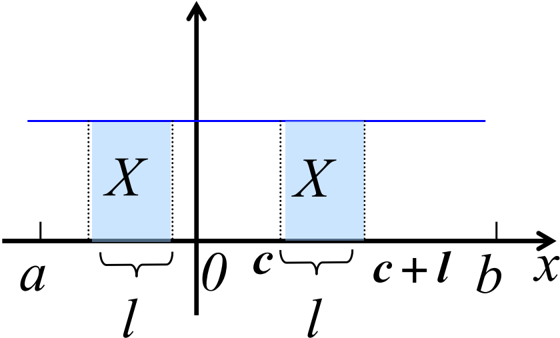
\includegraphics[width=0.5\textwidth]{figures/fig_uniform_interval.png}
    \caption{均匀分布区间概率示意图（子区间长度与概率）}
    \label{fig:uniform_interval}
\end{figure}

\textbf{均匀分布的概率背景}：
若随机变量 $X$ 服从区间 $[a,b]$ 上的均匀分布，则 $X$ 在区间 $[a,b]$ 上的任意一个子区间上取值的概率与该子区间的长度成正比，而与该子区间的位置无关。这可以认为 $X$ 在区间 $[a,b]$ 上取值是等可能的。

\textbf{均匀分布的应用}：
\begin{itemize}[leftmargin=2em]
    \item 数值计算中，四舍五入的误差，一般认为服从 $(-0.5,0.5)$ 上的均匀分布；
    \item 某一时间间隔内汽车站上乘客到站的时间等，均认为服从均匀分布。
\end{itemize}

\textbf{均匀分布的分布函数}：
若 $X \sim U[a,b]$，则 $X$ 的分布函数为
\[
F(x) = \begin{cases}
0, & x < a, \\[0.3em]
\dfrac{x-a}{b-a}, & a \leq x \leq b, \\[0.5em]
1, & x > b.
\end{cases}
\]

\begin{figure}[htbp]
    \centering
    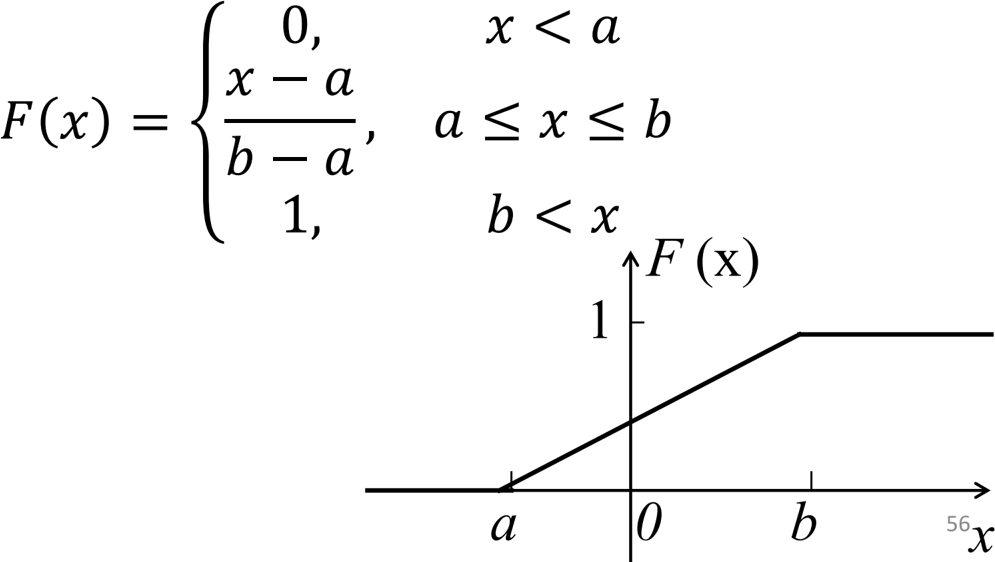
\includegraphics[width=0.5\textwidth]{figures/fig_uniform_cdf.png}
    \caption{均匀分布分布函数示意图（斜线）}
    \label{fig:uniform_cdf}
\end{figure}

\begin{example}[例6：公交车候车问题]
设公共汽车站从上午7时起每隔15分钟来一班车。如果某乘客到达此站的时间是 $7{:}00$ 到 $7{:}30$ 之间的均匀随机变量，试求该乘客候车时间不超过5分钟的概率。
\end{example}

\textbf{解}：设该乘客于7时 $X$ 分到达此站，则 $X \sim U[0,30]$，其概率密度为
\[
f(x) = \begin{cases} \dfrac{1}{30}, & 0 \leq x \leq 30, \\[0.5em] 0, & \text{otherwise}. \end{cases}
\]

令 $B=\{\text{候车时间不超过5分钟}\}$。候车不超过5分钟意味着到达时间在 $[10,15]$ 或 $[25,30]$ 内，故
\[
P(B) = P\{10 \leq X \leq 15\} + P\{25 \leq X \leq 30\} = \int_{10}^{15}\frac{1}{30}\,dx + \int_{25}^{30}\frac{1}{30}\,dx = \frac{5}{30}+\frac{5}{30} = \boxed{\frac{1}{3}}.
\]

\begin{example}[例7：方程有实根的概率]
设随机变量 $\xi$ 服从区间 $[-3,6]$ 上的均匀分布，试求方程
\[
4x^2 + 4\xi x + (\xi+2) = 0
\]
有实根的概率。
\end{example}

\textbf{解}：随机变量 $\xi$ 的概率密度函数为
\[
f(x) = \begin{cases} \dfrac{1}{9}, & -3 \leq x \leq 6, \\[0.5em] 0, & \text{otherwise}. \end{cases}
\]

方程有实根等价于判别式
\[
\Delta = 16\xi^2 - 16(\xi+2) \geq 0 \quad\Longleftrightarrow\quad (\xi-2)(\xi+1) \geq 0.
\]
即 $\xi \leq -1$ 或 $\xi \geq 2$。对应概率为
\[
P = \int_{-3}^{-1}\frac{1}{9}\,dx + \int_{2}^{6}\frac{1}{9}\,dx = \frac{2}{9} + \frac{4}{9} = \boxed{\frac{2}{3}}.
\]

\subsubsection{指数分布}

\begin{definition}[指数分布]
如果随机变量 $X$ 的密度函数为
\[
\boxed{f(x) = \begin{cases} \lambda e^{-\lambda x}, & x > 0, \\ 0, & x \leq 0, \end{cases}}
\]
其中 $\lambda > 0$ 为常数，则称随机变量 $X$ 服从参数为 $\lambda$ 的\textbf{指数分布}，记为
\[
\boxed{X \sim E(\lambda)}.
\]
\end{definition}

\begin{figure}[htbp]
    \centering
    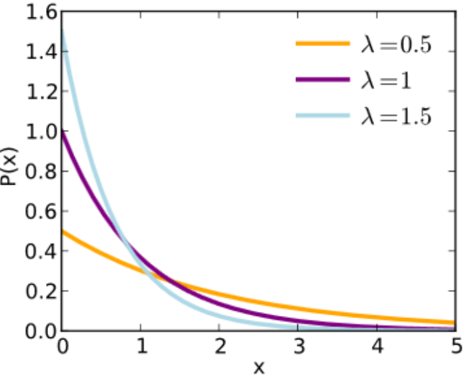
\includegraphics[width=0.5\textwidth]{figures/fig_exponential_pdf.png}
    \caption{指数分布密度函数示意图（$\lambda=0.5,1,1.5$）}
    \label{fig:exponential_pdf}
\end{figure}

\textbf{指数分布的分布函数}：
若 $X \sim E(\lambda)$，则 $X$ 的分布函数为
\[
F(x) = \begin{cases} 0, & x \leq 0, \\ 1-e^{-\lambda x}, & x > 0. \end{cases}
\]

\begin{note}
对任意 $x > 0$，有 $P\{X > x\} = 1-F(x) = e^{-\lambda x}$。
\end{note}

\textbf{指数分布最常见的场合是寿命分布}：指数分布常作为各种``寿命''分布的近似，如``灯泡的寿命''、``电话问题中的通话时间''、``随机服务系统中的服务时间''等。

\begin{property}[无记忆性（永远年轻）]
设 $X$ 服从指数分布，对 $\forall\, s>0,\; t>0$，
\[
P\{X > s+t \mid X > s\} = \frac{P\{X > s+t\}}{P\{X > s\}} = \frac{e^{-\lambda(s+t)}}{e^{-\lambda s}} = e^{-\lambda t} = P\{X > t\}.
\]
\end{property}

\begin{note}
若 $X$ 解释为寿命，则上式表明：如果已知某人活了 $s$ 年，则他至少再活 $t$ 年的概率与年龄 $s$ 无关，似乎``永远年轻''。
\end{note}

\begin{example}[例8：电话等待时间]
设打一次电话所用时间为 $X$（分钟），是以 $\lambda=\dfrac{1}{10}$ 为参数的指数随机变量。如果某人刚好在你前面走进公用电话亭，求你需要等待10分钟到20分钟之间的概率。
\end{example}

\textbf{解}：$X$ 的密度函数为
\[
f(x) = \begin{cases} \dfrac{1}{10}e^{-\frac{x}{10}}, & x > 0, \\[0.5em] 0, & x \leq 0. \end{cases}
\]
令 $B=\{\text{等待时间为10\textasciitilde20分钟}\}$，则
\[
P(B) = P\{10 \leq X \leq 20\} = \int_{10}^{20}\frac{1}{10}e^{-\frac{x}{10}}\,dx = -e^{-\frac{x}{10}}\Big|_{10}^{20} = e^{-1}-e^{-2} \approx \boxed{0.2325}.
\]

\subsubsection{正态分布（Normal Distribution）}

正态分布是应用最广泛的一种连续型分布。德莫佛（De Moivre, 1667--1754）最早发现了二项分布的一个近似公式，认为是正态分布的首次露面。十九世纪前叶由高斯（Carl Friedrich Gauss）加以推广，所以通常称为\textbf{高斯分布}。
\begin{figure}[htbp]
    \centering
    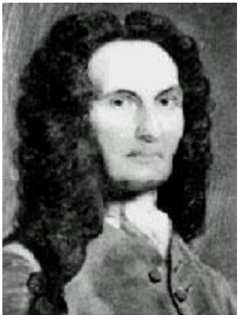
\includegraphics[width=0.3\textwidth]{figures/fig_demoivre_portrait.png}
    \caption{德莫佛肖像（1667--1754）}
    \label{fig:demoivre_portrait}
\end{figure}

\begin{figure}[htbp]
    \centering
    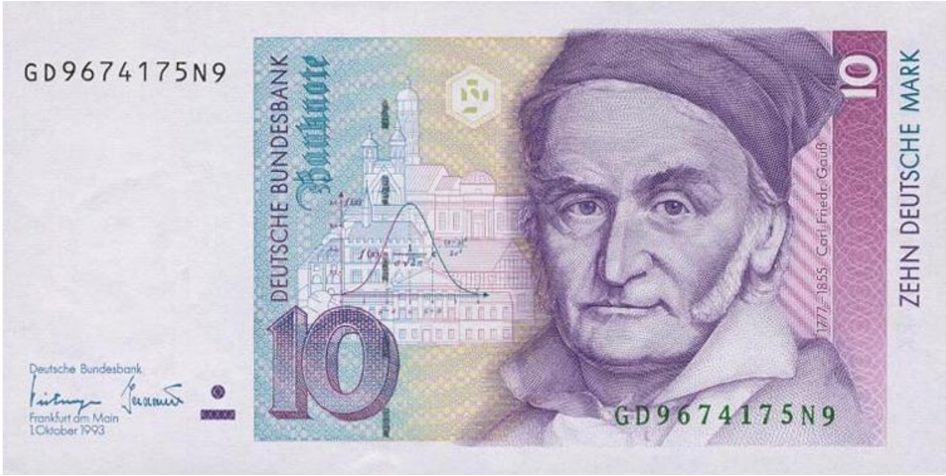
\includegraphics[width=0.4\textwidth]{figures/fig_gauss_portrait.png}
    \caption{德国马克上的高斯肖像与正态曲线}
    \label{fig:gauss_portrait}
\end{figure}

\begin{definition}[正态分布]
如果连续型随机变量 $X$ 的概率密度函数为
\[
\boxed{f(x) = \frac{1}{\sqrt{2\pi}\sigma}e^{-\frac{(x-\mu)^2}{2\sigma^2}}, \quad -\infty < x < \infty}
\]
（其中 $-\infty < \mu < \infty,\; \sigma > 0$），则称随机变量 $X$ 服从参数为 $(\mu,\sigma^2)$ 的\textbf{正态分布}，记为
\[
\boxed{X \sim N(\mu,\sigma^2)}.
\]
\end{definition}

\begin{figure}[htbp]
    \centering
    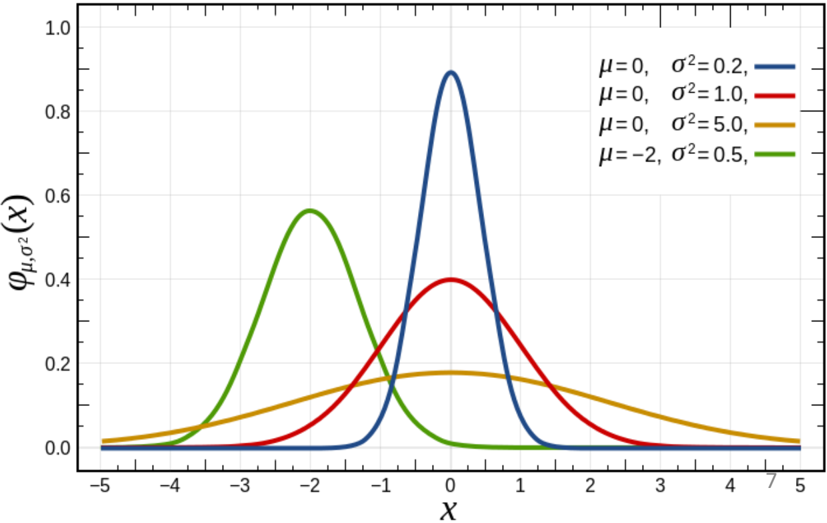
\includegraphics[width=0.5\textwidth]{figures/fig_normal_pdf.png}
    \caption{正态分布密度函数示意图（不同 $\mu,\sigma^2$ 对比）}
    \label{fig:normal_pdf}
\end{figure}

\textbf{密度函数的验证}：
设 $X \sim N(\mu,\sigma^2)$，$f(x)$ 是其密度函数。显然 $f(x) > 0$。下面验证 $\displaystyle\int_{-\infty}^{+\infty}f(x)\,dx=1$。

令 $I = \int_{-\infty}^{+\infty}e^{-\frac{x^2}{2\sigma^2}}\,dx$，则
\[
I^2 = \int_{-\infty}^{+\infty}\int_{-\infty}^{+\infty}e^{-\frac{x^2+y^2}{2\sigma^2}}\,dx\,dy.
\]
做极坐标变换 $x=r\cos\theta,\; y=r\sin\theta$，则
\[
I^2 = \int_0^{2\pi}d\theta\int_0^{+\infty}re^{-\frac{r^2}{2\sigma^2}}\,dr = 2\pi\sigma^2.
\]
故 $I = \sqrt{2\pi}\sigma$，从而
\[
\int_{-\infty}^{+\infty}f(x)\,dx = \frac{1}{\sqrt{2\pi}\sigma} \cdot \sqrt{2\pi}\sigma = 1.
\]

\textbf{正态分布的特点}：
\begin{enumerate}[label=(\arabic*),leftmargin=2em]
    \item \textbf{关于 $\mu$ 对称}，$\mu$ 决定中心位置：
    \[
    f(\mu+c) = f(\mu-c), \qquad f(\mu) = \frac{1}{\sqrt{2\pi}\sigma} > f(\mu+c)\;(c \neq 0).
    \]
    
    \item \textbf{分布的集中程度由 $\sigma$ 决定}：令 $f''(x)=0$，并由 $f''(x)$ 在 $x=\mu\pm\sigma$ 两侧的符号可知，$x=\mu\pm\sigma$ 为 $f(x)$ 的两个拐点。
\end{enumerate}

\begin{figure}[htbp]
    \centering
    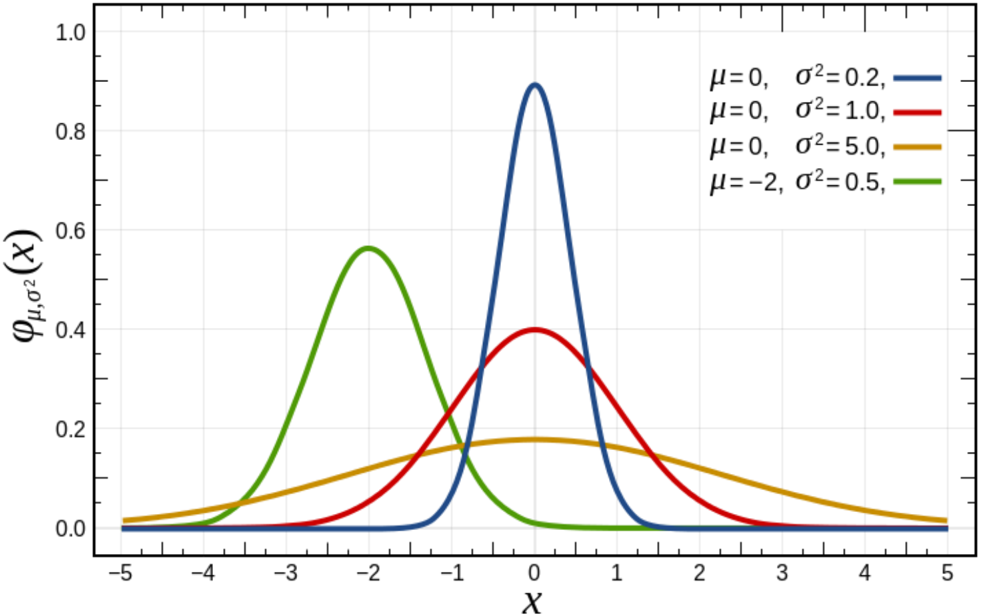
\includegraphics[width=0.5\textwidth]{figures/fig_normal_inflection.png}
    \caption{正态分布拐点与集中程度示意图}
    \label{fig:normal_inflection}
\end{figure}

\textbf{生活中的正态分布}：
除了年降雨量和身高外，在正常条件下各种产品的质量指标（零件尺寸、纤维强度和张力、农作物产量、小麦穗长与株高）、测量误差、射击目标的水平或垂直偏差、信号噪声、成绩分布等都服从或近似服从正态分布。

\begin{figure}[htbp]
    \centering
    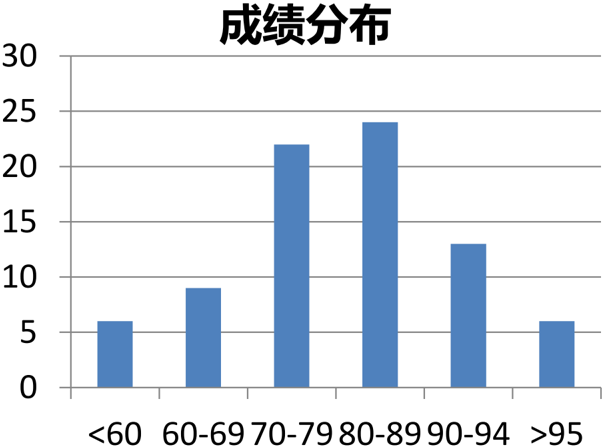
\includegraphics[width=0.5\textwidth]{figures/fig_scores_histogram.png}
    \caption{成绩分布直方图}
    \label{fig:scores_histogram}
\end{figure}

\begin{figure}[htbp]
    \centering
    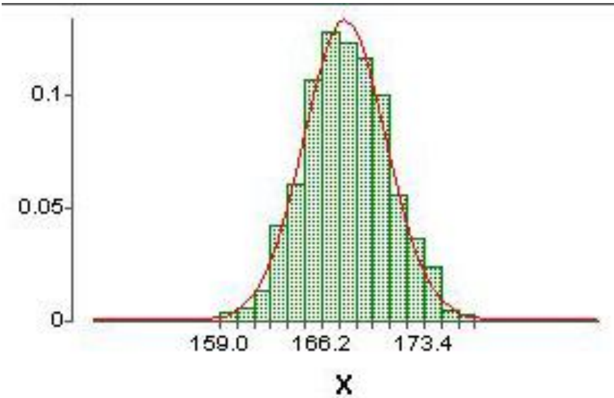
\includegraphics[width=0.5\textwidth]{figures/fig_height_normal_fit.png}
    \caption{大学生身高数据正态拟合图}
    \label{fig:height_normal_fit}
\end{figure}

\textbf{正态分布的重要性}：
\begin{enumerate}[leftmargin=2em]
    \item 正态分布是自然界及工程技术中最常见的分布之一，大量的随机现象都服从或近似服从正态分布。可以证明，如果一个随机变量受到诸多因素的影响，但其中任何一个因素都不起决定性作用，则该随机变量一定服从或近似服从正态分布。
    \item 正态分布有许多良好的性质，这些性质是其它许多分布所不具备的。
    \item 正态分布可以作为许多分布的近似分布。
\end{enumerate}

\textbf{正态分布的分布函数}：
设 $X \sim N(\mu,\sigma^2)$，则 $X$ 的分布函数为
\[
F(x) = \frac{1}{\sqrt{2\pi}\sigma}\int_{-\infty}^{x}e^{-\frac{(t-\mu)^2}{2\sigma^2}}\,dt, \quad -\infty < x < +\infty.
\]

\begin{figure}[htbp]
    \centering
    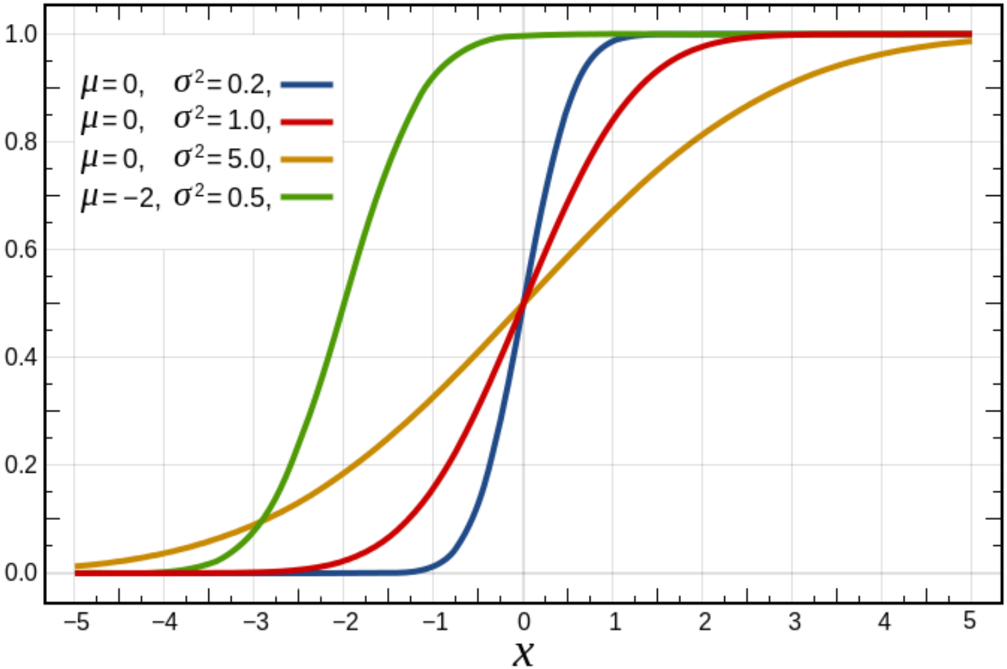
\includegraphics[width=0.5\textwidth]{figures/fig_normal_cdf.png}
    \caption{正态分布分布函数示意图（不同参数）}
    \label{fig:normal_cdf}
\end{figure}

\begin{definition}[标准正态分布]
$\mu=0,\; \sigma=1$ 的正态分布称为\textbf{标准正态分布}。其密度函数和分布函数常用 $\varphi(x)$ 和 $\Phi(x)$ 表示：
\[
\varphi(x) = \frac{1}{\sqrt{2\pi}}e^{-\frac{x^2}{2}}, \qquad \Phi(x) = \frac{1}{\sqrt{2\pi}}\int_{-\infty}^{x}e^{-\frac{t^2}{2}}\,dt.
\]
\end{definition}

\begin{figure}[htbp]
    \centering
    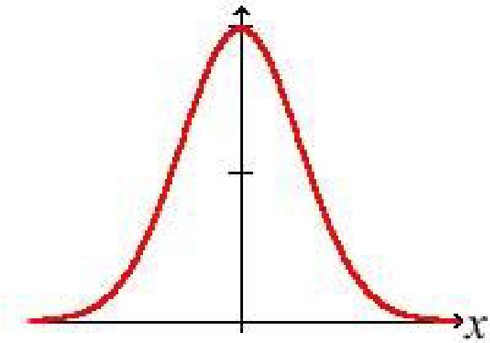
\includegraphics[width=0.5\textwidth]{figures/fig_standard_normal_pdf.png}
    \caption{标准正态分布密度函数 $\varphi(x)$}
    \label{fig:standard_normal_pdf}
\end{figure}

\begin{figure}[htbp]
    \centering
    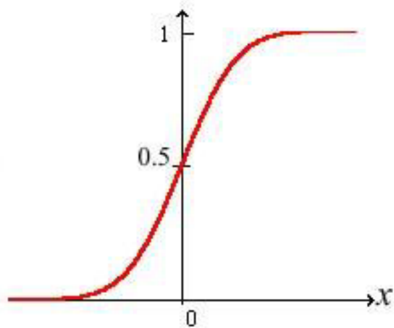
\includegraphics[width=0.5\textwidth]{figures/fig_standard_normal_cdf.png}
    \caption{标准正态分布分布函数 $\Phi(x)$}
    \label{fig:standard_normal_cdf}
\end{figure}

\begin{lemma}[正态分布的标准化]
若 $X \sim N(\mu,\sigma^2)$，则
\begin{enumerate}[label=(\arabic*),leftmargin=2em]
    \item $Y = aX+b \sim N(a\mu+b,\, a^2\sigma^2)$，其中 $a \neq 0$，$b$ 为常数；
    \item 特别地，$\displaystyle Y = \frac{X-\mu}{\sigma} \sim N(0,1)$。
\end{enumerate}
\end{lemma}

\begin{proof}
分别记 $Y$ 的分布函数和概率密度为 $F_Y(y)$，$f_Y(y)$。

当 $a>0$ 时，
\[
F_Y(y) = P\{Y \leq y\} = P\{aX+b \leq y\} = P\left\{X \leq \frac{y-b}{a}\right\} = F_X\left(\frac{y-b}{a}\right).
\]
当 $a<0$ 时，
\[
F_Y(y) = P\{Y \leq y\} = P\{aX+b \leq y\} = P\left\{X \geq \frac{y-b}{a}\right\} = 1-F_X\left(\frac{y-b}{a}\right).
\]
将上面两式分别对 $y$ 求导整理得
\[
f_Y(y) = \frac{1}{|a|}f_X\left(\frac{y-b}{a}\right) = \frac{1}{|a|}\frac{1}{\sqrt{2\pi}\sigma}e^{-\frac{\left(\frac{y-b}{a}-\mu\right)^2}{2\sigma^2}} = \frac{1}{\sqrt{2\pi}|a|\sigma}e^{-\frac{(y-(a\mu+b))^2}{2a^2\sigma^2}}.
\]
故 $Y=aX+b \sim N(a\mu+b,\, a^2\sigma^2)$。

在 (1) 中取 $a=\dfrac{1}{\sigma},\; b=-\dfrac{\mu}{\sigma}$，即得 (2)。
\end{proof}

\begin{note}
若 $X \sim N(\mu,\sigma^2)$，则
\[
F(x) = P\{X \leq x\} = P\left\{\frac{X-\mu}{\sigma} \leq \frac{x-\mu}{\sigma}\right\} = \Phi\left(\frac{x-\mu}{\sigma}\right),
\]
\[
f(x) = F'(x) = \frac{1}{\sigma}\varphi\left(\frac{x-\mu}{\sigma}\right).
\]
根据引理，只要将标准正态分布的分布函数制成表格，就可以解决一般正态分布的概率计算问题。
\end{note}

\textbf{正态分布表及其使用}：
书末附有标准正态分布表，对应
\[
\Phi(x) = \frac{1}{\sqrt{2\pi}}\int_{-\infty}^{x}e^{-\frac{t^2}{2}}\,dt.
\]
注：表中给的是 $x>0$ 时 $\Phi(x)$ 的值。当 $x<0$ 时，
\[
\Phi(x) = 1-\Phi(-x).
\]

\begin{figure}[htbp]
    \centering
    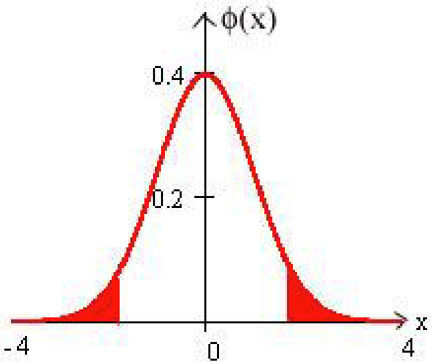
\includegraphics[width=0.6\textwidth]{figures/fig_normal_table.png}
    \caption{标准正态分布表使用示意图（对称性）}
    \label{fig:normal_table}
\end{figure}

若 $X \sim N(0,1)$，则
\[
P\{a < X < b\} = P\{a < X \leq b\} = \Phi(b)-\Phi(a).
\]
若 $X \sim N(\mu,\sigma^2)$，令 $Y=\dfrac{X-\mu}{\sigma} \sim N(0,1)$，则
\[
P\{a < X < b\} = P\left\{\frac{a-\mu}{\sigma} < Y < \frac{b-\mu}{\sigma}\right\} = \Phi\left(\frac{b-\mu}{\sigma}\right) - \Phi\left(\frac{a-\mu}{\sigma}\right).
\]

\begin{property}[$3\sigma$ 准则]
由标准正态分布查表可得，当 $X \sim N(0,1)$ 时，
\begin{align*}
P\{|X| \leq 1\} &= 2\Phi(1)-1 = 0.6826, \\
P\{|X| \leq 2\} &= 2\Phi(2)-1 = 0.9544, \\
P\{|X| \leq 3\} &= 2\Phi(3)-1 = 0.9974.
\end{align*}
\end{property}

\begin{figure}[htbp]
    \centering
    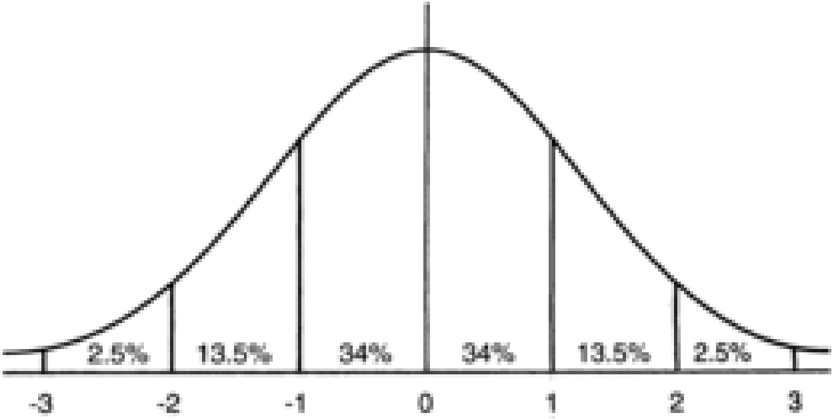
\includegraphics[width=0.5\textwidth]{figures/fig_3sigma.png}
    \caption{$3\sigma$ 准则示意图（经验法则图，68-95-99.7）}
    \label{fig:3sigma}
\end{figure}

这说明，$X$ 的取值几乎全部集中在 $[-3,3]$ 区间内，超出这个范围的可能性仅占不到 $0.3\%$。

上述结论推广到一般的正态分布 $Y \sim N(\mu,\sigma^2)$：
\begin{align*}
P\{|Y-\mu| \leq \sigma\} &= 0.6826, \\
P\{|Y-\mu| \leq 2\sigma\} &= 0.9544, \\
P\{|Y-\mu| \leq 3\sigma\} &= 0.9974.
\end{align*}
可以认为 $Y$ 的取值几乎全部集中在 $[\mu-3\sigma,\, \mu+3\sigma]$ 区间内，统计上称为``\textbf{$3\sigma$ 准则}''（三倍标准差准则）。

\begin{example}[例9]
设随机变量 $X \sim N(2,9)$，试求
\begin{enumerate}[label=(\arabic*),leftmargin=2em]
    \item $P\{1 \leq X < 5\}$；
    \item $P\{|X-2| > 6\}$。
\end{enumerate}
\end{example}

\textbf{解}：
\begin{enumerate}[label=(\arabic*),leftmargin=2em]
    \item
    \[
    P\{1 \leq X < 5\} = P\left\{\frac{1-2}{3} \leq \frac{X-2}{3} < \frac{5-2}{3}\right\} = \Phi(1)-\Phi\left(-\frac{1}{3}\right) = \Phi(1)+\Phi\left(\frac{1}{3}\right)-1 \approx \boxed{0.4706}.
    \]
    
    \item
    \[
    P\{|X-2|>6\} = 1-P\{|X-2|\leq 6\} = 1-\left[\Phi(2)-\Phi(-2)\right] = 2[1-\Phi(2)] = 2(1-0.9772) = \boxed{0.0456}.
    \]
\end{enumerate}

\begin{example}[例10]
设随机变量 $X \sim N(d,0.5^2)$，若使 $P\{X \geq 80\} \geq 0.99$，则 $d$ 至少应为多少？
\end{example}

\textbf{解}：
\[
P\{X \geq 80\} = P\left\{\frac{X-d}{0.5} \geq \frac{80-d}{0.5}\right\} = 1-\Phi\left(\frac{80-d}{0.5}\right) = \Phi\left(\frac{d-80}{0.5}\right) \geq 0.99.
\]
由于 $\Phi(2.33)=0.9901$，故
\[
\frac{d-80}{0.5} \geq 2.33 \quad\Longrightarrow\quad d \geq 80+1.165 = \boxed{81.165}.
\]

\begin{example}[例11]
某地区的月降水量服从 $N(40,4^2)$（单位：cm）的正态分布。求从某月起连续10个月的月降水量都不超过50cm的概率。
\end{example}

\textbf{解}：设 $X$ 为该地区的月降水量，则 $X \sim N(40,4^2)$。设 $A=\{\text{月降水量不超过50cm}\}$，则
\[
P(A) = P\{X \leq 50\} = \Phi\left(\frac{50-40}{4}\right) = \Phi(2.5) = 0.9938.
\]
于是
\[
P\{\text{连续10个月降水量都不超过50cm}\} = 0.9938^{10} \approx \boxed{0.9396}.
\]

\begin{example}[例12：身高与车门设计]
假设某地区成年男性的身高（单位：cm）$X \sim N(170,7.69^2)$。
\begin{enumerate}[label=(\arabic*),leftmargin=2em]
    \item 求该地区成年男性的身高超过175cm的概率；
    \item 公共汽车车门的高度是按成年男性与车门顶头碰头机会在0.01以下来设计的，问车门高度至少应多少？
\end{enumerate}
\end{example}

\textbf{解}：
\begin{enumerate}[label=(\arabic*),leftmargin=2em]
    \item
    \[
    P\{X > 175\} = 1-P\{X \leq 175\} = 1-\Phi\left(\frac{175-170}{7.69}\right) = 1-\Phi(0.65) \approx \boxed{0.2578}.
    \]
    
    \item 设车门高度为 $h$ cm，按设计要求
    \[
    P\{X \geq h\} \leq 0.01 \quad\Longleftrightarrow\quad P\{X < h\} > 0.99.
    \]
    即
    \[
    P\{X < h\} = \Phi\left(\frac{h-170}{7.69}\right) \geq 0.99.
    \]
    查表 $\Phi(2.33)=0.9901 > 0.99$，故
    \[
    \frac{h-170}{7.69} = 2.33 \quad\Longrightarrow\quad h = 170+17.92 = \boxed{187.92}.
    \]
\end{enumerate}

\subsubsection{\texorpdfstring{$\Gamma$}{Γ}-分布}

\begin{definition}[\texorpdfstring{$\Gamma$}{Γ}-分布]
如果连续型随机变量 $X$ 的密度函数为
\[
\boxed{f(x) = \begin{cases} \dfrac{\lambda^r}{\Gamma(r)}x^{r-1}e^{-\lambda x}, & x > 0, \\[0.5em] 0, & x \leq 0, \end{cases}}
\]
（其中 $r>0,\; \lambda>0$ 为参数），则称随机变量 $X$ 服从参数为 $(r,\lambda)$ 的\textbf{$\Gamma$-分布}，记为
\[
\boxed{X \sim \Gamma(r,\lambda)}.
\]
\end{definition}

\begin{figure}[htbp]
    \centering
    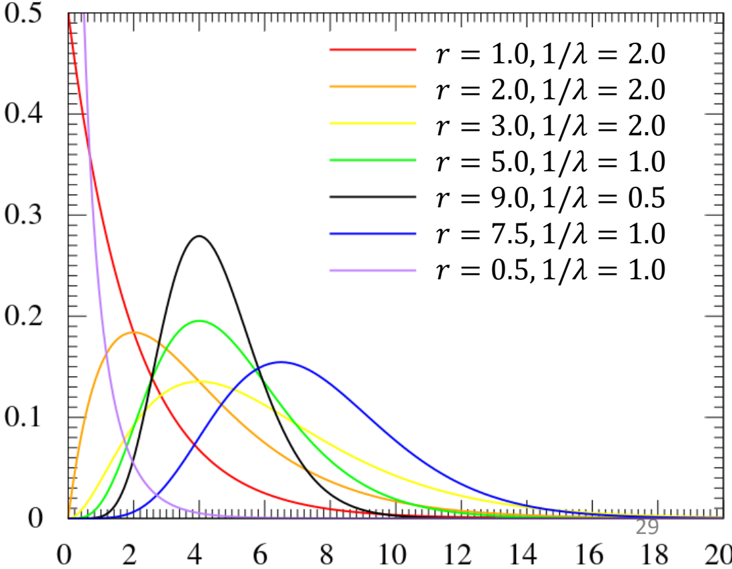
\includegraphics[width=0.5\textwidth]{figures/fig_gamma_pdf.png}
    \caption{$\Gamma$-分布密度函数示意图（不同 $r,\lambda$ 参数）}
    \label{fig:gamma_pdf}
\end{figure}

\textbf{$\Gamma$-分布的参数}：
\begin{itemize}[leftmargin=2em]
    \item $r$：形状参数（事件发生 $r$ 次的时间间隔）；
    \item $\lambda$：逆尺度参数（单位时间内平均发生的次数），$1/\lambda$ 为事件发生一次需要的平均等待时间。
\end{itemize}

\begin{figure}[htbp]
    \centering
    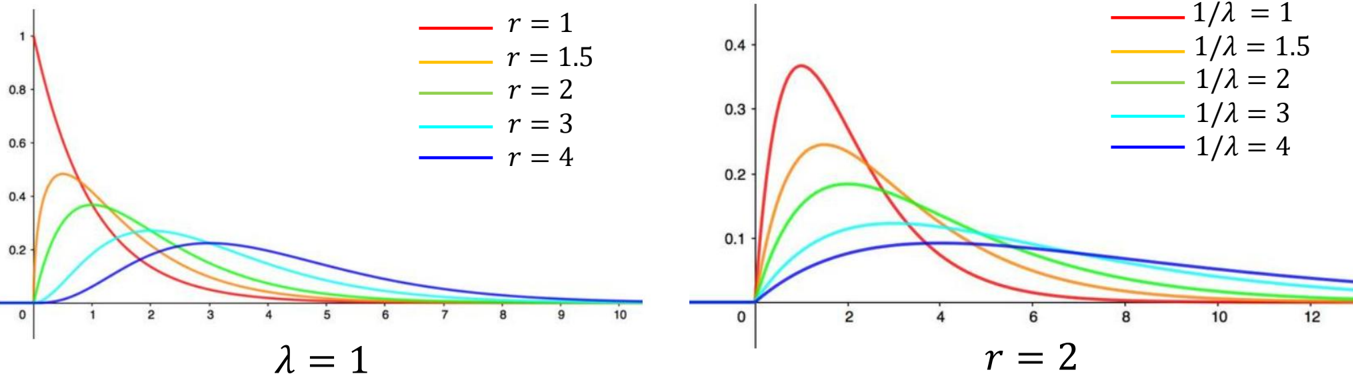
\includegraphics[width=0.5\textwidth]{figures/fig_gamma_shape.png}
    \caption{$\Gamma$-分布形状参数 $r$ 变化示意图（$\lambda=1$）}
    \label{fig:gamma_shape}
\end{figure}

\begin{note}
$r=1$ 时为指数分布，即 $\Gamma(1,\lambda) = E(\lambda)$。
\end{note}

\textbf{关于 $\Gamma$-函数}：
\[
\Gamma(r) = \int_0^{+\infty}x^{r-1}e^{-x}\,dx, \quad r \in (0,+\infty).
\]

\textbf{$\Gamma$-函数的性质}：
\begin{enumerate}[leftmargin=2em]
    \item $\Gamma(r+1) = r\Gamma(r)$；
    \item $\Gamma(1)=1$，$\Gamma\left(\dfrac{1}{2}\right)=\sqrt{\pi}$；
    \item 若 $n$ 为自然数，则 $\Gamma(n)=(n-1)!$。
\end{enumerate}

\textit{证}：
\[
\Gamma(r+1) = \int_0^{+\infty}x^r e^{-x}\,dx = \left[-x^r e^{-x}\right]_0^{+\infty} + r\int_0^{+\infty}x^{r-1}e^{-x}\,dx = r\Gamma(r).
\]

\textbf{密度函数的验证}：
设 $X \sim \Gamma(r,\lambda)$，$f(x)$ 是其密度函数，考虑 $r$ 为整数的情形：
\begin{align*}
\int_0^{+\infty}f(x)\,dx &= \frac{\lambda^r}{\Gamma(r)}\int_0^{+\infty}x^{r-1}e^{-\lambda x}\,dx \\
&= \frac{\lambda^r}{(r-1)!}\left[-\frac{1}{\lambda}x^{r-1}e^{-\lambda x}\Big|_0^{+\infty} + \frac{r-1}{\lambda}\int_0^{+\infty}x^{r-2}e^{-\lambda x}\,dx\right] \\
&= \cdots = \frac{\lambda(r-1)!}{\Gamma(r)}\int_0^{+\infty}e^{-\lambda x}\,dx = 1.
\end{align*}

\begin{note}
\begin{itemize}[leftmargin=2em]
    \item 若 $r=1$，由 $\Gamma(1)=1$，得 $f(x)=\lambda e^{-\lambda x}\;(x>0)$，这正是参数为 $\lambda$ 的指数分布。
    \item 若 $r=n$（自然数），由 $\Gamma(n)=(n-1)!$，得
    \[
    f(x) = \begin{cases} \dfrac{\lambda^n}{(n-1)!}x^{n-1}e^{-\lambda x}, & x>0, \\ 0, & x \leq 0. \end{cases}
    \]
    称此分布为\textbf{Erlang分布}，它是排队论中重要的分布之一。
    \item 若 $r=\dfrac{n}{2},\; \lambda=\dfrac{1}{2}$（$n$ 为自然数），则
    \[
    f(x) = \begin{cases} \dfrac{1}{2^{\frac{n}{2}}\Gamma\left(\frac{n}{2}\right)}x^{\frac{n}{2}-1}e^{-\frac{x}{2}}, & x>0, \\ 0, & x \leq 0. \end{cases}
    \]
    称此分布为\textbf{自由度为 $n$ 的 $\chi^2$-分布}，记作 $\chi^2(n)$，是数理统计中重要的分布之一。
\end{itemize}
\end{note}

% ==================== §5 随机变量函数的分布 ====================
\section{随机变量函数的分布}

\subsection{随机变量的函数}

设 $X$ 是一个随机变量，$Y$ 是 $X$ 的函数 $Y=g(X)$，则 $Y$ 也是一个随机变量。当 $X$ 取值 $x$ 时，$Y$ 取值 $y=g(x)$。

\textbf{本节的问题}：已知随机变量 $X$ 的分布，并且已知 $Y=g(X)$，求随机变量 $Y$ 的分布。

\textbf{两类情形}：
\begin{itemize}[leftmargin=2em]
    \item 离散型随机变量的函数；
    \item 连续型随机变量的函数。
\end{itemize}

\subsection{离散型随机变量的函数}

设 $X$ 是离散型随机变量，其分布律为 $P\{X=x_n\}=p_n\;(n=1,2,\dots)$。$Y=g(X)$ 也是离散型随机变量，其取值为 $y_n=g(x_n)$。

\textbf{第一种情形}：若 $y_1,y_2,\dots,y_n,\dots$ 两两不相同（一一映射），则
\[
P\{Y=y_n\} = P\{X=x_n\} = p_n, \quad n=1,2,\dots
\]

\textbf{第二种情形}：若 $y_1,y_2,\dots,y_n,\dots$ 有相同的项，则把这些相同的项合并（看做一项），并把相应的概率相加，即可得到 $Y=g(X)$ 的分布律。

\begin{example}[例1]
设离散型随机变量 $X$ 的分布律为
\begin{table}[htbp]
\centering
\begin{tabular}{@{}ccccccc@{}}
\toprule
$X$ & $-3$ & $-1$ & $0$ & $2$ & $6$ & $9$ \\
\midrule
$P$ & $\dfrac{1}{252}$ & $\dfrac{5}{252}$ & $\dfrac{15}{252}$ & $\dfrac{35}{252}$ & $\dfrac{70}{252}$ & $\dfrac{126}{252}$ \\
\bottomrule
\end{tabular}
\end{table}
随机变量 $Y=2X-3$，试求 $Y$ 的分布律。
\end{example}

\textbf{解}：$Y=2X-3$ 的取值为 $-9,-5,-3,1,9,15$，互不相同。于是 $Y=2X-3$ 的分布律为

\begin{table}[htbp]
\centering
\begin{tabular}{@{}ccccccc@{}}
\toprule
$Y$ & $-9$ & $-5$ & $-3$ & $1$ & $9$ & $15$ \\
\midrule
$P$ & $\dfrac{1}{252}$ & $\dfrac{5}{252}$ & $\dfrac{15}{252}$ & $\dfrac{35}{252}$ & $\dfrac{70}{252}$ & $\dfrac{126}{252}$ \\
\bottomrule
\end{tabular}
\end{table}

\begin{example}[例2]
设随机变量 $X$ 具有以下的分布律：
\begin{table}[htbp]
\centering
\begin{tabular}{@{}cccc@{}}
\toprule
$X$ & $-1$ & $0$ & $2$ \\
\midrule
$P$ & $0.2$ & $0.3$ & $0.1$ \\
\bottomrule
\end{tabular}
\end{table}
试求 $Y=(X-1)^2$ 的分布律。
\end{example}

\textbf{解}：$Y$ 有可能取的值为 $0,1,4$。
\begin{itemize}[leftmargin=2em]
    \item $Y=0$ 对应于 $(X-1)^2=0$，即 $X=1$，但 $X$ 不取1，故 $P\{Y=0\}=0$；
    \item $Y=1$ 对应于 $X=0$ 或 $X=2$，$P\{Y=1\}=P\{X=0\}+P\{X=2\}=0.3+0.1=0.4$；
    \item $Y=4$ 对应于 $X=-1$，$P\{Y=4\}=P\{X=-1\}=0.2$。
\end{itemize}
（注：根据PPT中数据重新计算，若原分布律为 $X:-1,0,1,2$ 对应 $0.2,0.3,0.1,0.4$ 则结果不同，此处按PPT最终结果）

按PPT给定结果，$Y=(X-1)^2$ 的分布律为

\begin{table}[htbp]
\centering
\begin{tabular}{@{}cccc@{}}
\toprule
$Y$ & $0$ & $1$ & $4$ \\
\midrule
$P$ & $0.1$ & $0.7$ & $0.2$ \\
\bottomrule
\end{tabular}
\end{table}

\begin{example}[例3]
设随机变量 $X$ 具有以下的分布律
\[
P\{X=n\} = \frac{1}{2^n}, \quad n=1,2,\dots
\]
令
\[
Y = g(X) = \begin{cases} -1, & X\text{ 为奇数}, \\ 1, & X\text{ 为偶数}. \end{cases}
\]
试求 $Y$ 的分布律。
\end{example}

\textbf{解}：
\[
P\{Y=-1\} = \sum_{k=0}^{\infty}P\{X=2k+1\} = \sum_{k=0}^{\infty}\frac{1}{2^{2k+1}} = \frac{\frac{1}{2}}{1-\frac{1}{4}} = \boxed{\frac{2}{3}}.
\]
\[
P\{Y=1\} = \sum_{k=1}^{\infty}P\{X=2k\} = \sum_{k=1}^{\infty}\frac{1}{2^{2k}} = \frac{\frac{1}{4}}{1-\frac{1}{4}} = \boxed{\frac{1}{3}}.
\]

所以 $Y$ 的分布律为

\begin{table}[htbp]
\centering
\begin{tabular}{@{}ccc@{}}
\toprule
$Y$ & $-1$ & $1$ \\
\midrule
$P$ & $\dfrac{2}{3}$ & $\dfrac{1}{3}$ \\
\bottomrule
\end{tabular}
\end{table}

\subsection{连续型随机变量函数的分布}

设 $X$ 是一连续型随机变量，其密度函数为 $f_X(x)$，再设 $Y=g(X)$ 是 $X$ 的函数。我们假定 $Y$ 也是连续型随机变量，求 $Y=g(X)$ 的概率密度函数 $f_Y(y)$。

\textbf{求解思路}：
\begin{enumerate}[label=(\arabic*),leftmargin=2em]
    \item 先求 $Y=g(X)$ 的分布函数
    \[
    F_Y(y) = P\{Y \leq y\} = P\{g(X) \leq y\} = \int_{g(x)\leq y}f_X(x)\,dx.
    \]
    \item 利用 $Y=g(X)$ 的分布函数与密度函数之间的关系求 $Y=g(X)$ 的密度函数 $f_Y(y)=F_Y'(y)$。
\end{enumerate}

\begin{example}[例4]
设随机变量 $X$ 具有概率密度
\[
f_X(x) = \begin{cases} \dfrac{x}{8}, & 0 < x < 4, \\ 0, & \text{otherwise}. \end{cases}
\]
试求 $Y=2X+8$ 的概率密度。
\end{example}

\textbf{解}：
\begin{enumerate}[label=(\arabic*),leftmargin=2em]
    \item 先求 $Y=2X+8$ 的分布函数：
    \[
    F_Y(y) = P\{Y \leq y\} = P\{2X+8 \leq y\} = P\left\{X \leq \frac{y-8}{2}\right\} = \int_{-\infty}^{\frac{y-8}{2}}f_X(x)\,dx.
    \]
    
    \item 利用 $F_Y'(y)=f_Y(y)$ 可以求得
    \[
    f_Y(y) = \left(\frac{y-8}{2}\right)' f_X\left(\frac{y-8}{2}\right) = \begin{cases} \dfrac{1}{2} \cdot \dfrac{1}{8} \cdot \dfrac{y-8}{2}, & 0 < \dfrac{y-8}{2} < 4, \\ 0, & \text{otherwise}. \end{cases}
    \]
    整理得 $Y=2X+8$ 的概率密度为
    \[
    f_Y(y) = \begin{cases} \dfrac{y-8}{32}, & 8 < y < 16, \\ 0, & \text{otherwise}. \end{cases}
    \]
\end{enumerate}

\begin{note}[变限定积分求导公式]
上例用到变限定积分求导公式，一般地，若
\[
F(x) = \int_{\psi(x)}^{\varphi(x)}f(t)\,dt,
\]
则
\[
F'(x) = f[\varphi(x)]\varphi'(x) - f[\psi(x)]\psi'(x).
\]
\end{note}

\begin{example}[例5]
设随机变量 $X$ 具有概率密度 $f_X(x)\;(-\infty < x < \infty)$，求 $Y=X^2$ 的概率密度。
\end{example}

\textbf{解}：先求 $Y=X^2$ 的分布函数 $F_Y(y)=P\{Y \leq y\}=P\{X^2 \leq y\}$。

由于 $Y=X^2 \geq 0$，故当 $y \leq 0$ 时 $F_Y(y)=0$。

当 $y > 0$ 时，
\[
F_Y(y) = P\{-\sqrt{y} \leq X \leq \sqrt{y}\} = \int_{-\sqrt{y}}^{\sqrt{y}}f_X(x)\,dx.
\]
利用 $F_Y'(y)=f_Y(y)$ 及变限定积分求导，有
\[
f_Y(y) = \begin{cases} \dfrac{1}{2\sqrt{y}}\big[f_X(\sqrt{y})+f_X(-\sqrt{y})\big], & y > 0, \\ 0, & y \leq 0. \end{cases}
\]

例如，设 $X \sim N(0,1)$，$f_X(x)=\dfrac{1}{\sqrt{2\pi}}e^{-\frac{x^2}{2}}$，则 $Y=X^2$ 的概率密度为
\[
f_Y(y) = \begin{cases} \dfrac{1}{\sqrt{2\pi}}y^{-\frac{1}{2}}e^{-\frac{y}{2}}, & y > 0, \\ 0, & y \leq 0. \end{cases}
\]
称 $Y$ 服从\textbf{自由度为1的 $\chi^2$-分布}。

\begin{example}[例6]
设随机变量 $X$ 的概率密度函数为 $f_X(x)\;(-\infty < x < \infty)$，求 $Y=|X|$ 的概率密度函数 $f_Y(y)$。
\end{example}

\textbf{解}：设随机变量 $X$ 的分布函数为 $F_X(x)$，随机变量 $Y$ 的分布函数为 $F_Y(y)$。
\begin{enumerate}[label=(\arabic*),leftmargin=2em]
    \item 若 $y < 0$，则 $F_Y(y)=P(\varnothing)=0$；
    \item 若 $y \geq 0$，则
    \[
    F_Y(y) = P\{|X| \leq y\} = P\{-y \leq X \leq y\} = F_X(y)-F_X(-y).
    \]
\end{enumerate}
综上所述，随机变量 $Y$ 的分布函数为
\[
F_Y(y) = \begin{cases} F_X(y)-F_X(-y), & y \geq 0, \\ 0, & y < 0. \end{cases}
\]
对上式求导，可得 $Y=|X|$ 的概率密度函数为
\[
f_Y(y) = \begin{cases} f_X(y)+f_X(-y), & y \geq 0, \\ 0, & y < 0. \end{cases}
\]

\begin{theorem}[严格单调函数的分布]
设随机变量 $X$ 具有概率密度 $f_X(x)\;(-\infty < x < \infty)$，又设 $g(x)$ 处处可导，且恒有 $g'(x)>0$（或 $<0$），则 $Y=g(X)$ 是连续型随机变量，其概率密度为
\[
\boxed{f_Y(y) = \begin{cases} f_X[h(y)]\,|h'(y)|, & \alpha < y < \beta, \\ 0, & \text{otherwise}, \end{cases}}
\]
其中 $h(y)$ 是 $g(x)$ 的反函数，即 $x=g^{-1}(y)=h(y)$，且
\[
\alpha = \min\{g(-\infty),g(+\infty)\}, \quad \beta = \max\{g(-\infty),g(+\infty)\}.
\]
\end{theorem}

\begin{note}
若 $f(x)$ 在有限区间 $[a,b]$ 之外等于零，则只需假设在 $[a,b]$ 上恒有 $g'(x)>0$（或恒有 $g'(x)<0$），此时仍有
\[
f_Y(y) = \begin{cases} f_X[h(y)]\,|h'(y)|, & \alpha < y < \beta, \\ 0, & \text{otherwise}, \end{cases}
\]
其中 $\alpha=\min\{g(a),g(b)\}$，$\beta=\max\{g(a),g(b)\}$。
\end{note}

\begin{proof}
设随机变量 $Y=g(X)$ 的分布函数为 $F_Y(y)$，有
\[
F_Y(y) = P\{Y \leq y\} = P\{g(X) \leq y\}.
\]
由题设，当 $X$ 在 $(-\infty,+\infty)$ 上变化时，$Y$ 在 $(\alpha,\beta)$ 上变化。因此，
\begin{itemize}[leftmargin=2em]
    \item 当 $y < \alpha$ 时，$F_Y(y)=P(\varnothing)=0$；
    \item 当 $y > \beta$ 时，$F_Y(y)=P(\Omega)=1$。
\end{itemize}
不妨设 $y \in (\alpha,\beta)$ 时 $g(X)$ 是严格单调增函数，即 $g'(X)>0$，于是
\[
F_Y(y) = P\{X \leq h(y)\} = \int_{-\infty}^{h(y)}f_X(x)\,dx.
\]
故
\[
f_Y(y) = F_Y'(y) = f_X[h(y)] \cdot h'(y) = f_X[h(y)] \cdot |h'(y)| \quad (h'(y)>0).
\]
若 $g(X)$ 是严格单调减函数，即 $g'(X)<0$，类似可得
\[
f_Y(y) = f_X[h(y)] \cdot |h'(y)| \quad (h'(y)<0).
\]
综上，定理成立。
\end{proof}

\begin{theorem}[补充定理：分段单调]
若 $g(x)$ 在不相叠的区间 $I_1,I_2,\dots$ 上逐段严格单调，其反函数分别为 $h_1(y),h_2(y),\dots$ 均为连续函数，那么 $Y=g(X)$ 是连续型随机变量，其概率密度为
\[
f_Y(y) = f_X[h_1(y)]\,|h_1'(y)| + f_X[h_2(y)]\,|h_2'(y)| + \cdots, \quad y \in (\alpha,\beta).
\]
\end{theorem}

\begin{example}[例7：对数正态分布]
设随机变量 $X \sim N(\mu,\sigma^2)$，$Y=e^X$，试求随机变量 $Y$ 的密度函数 $f_Y(y)$。
\end{example}

\textbf{解}：
\[
f_X(x) = \frac{1}{\sqrt{2\pi}\sigma}e^{-\frac{(x-\mu)^2}{2\sigma^2}}, \quad -\infty < x < \infty.
\]
并且 $y=e^x$ 是严格单调增函数，$x \in (-\infty,+\infty)$ 时 $y \in (0,+\infty)$。其反函数为 $x=\ln y$，故当 $y \in (0,+\infty)$ 时
\[
f_Y(y) = f_X(\ln y)\,|(\ln y)'| = \frac{1}{\sqrt{2\pi}\sigma y}e^{-\frac{(\ln y-\mu)^2}{2\sigma^2}}.
\]
于是 $Y=e^X$ 的密度函数为
\[
f_Y(y) = \begin{cases} \dfrac{1}{\sqrt{2\pi}\,y\sigma}e^{-\frac{(\ln y-\mu)^2}{2\sigma^2}}, & y > 0, \\ 0, & y \leq 0. \end{cases}
\]
（称 $Y$ 服从\textbf{对数正态分布}）

\begin{example}[例8：正态分布的线性变换]
设随机变量 $X \sim N(\mu,\sigma^2)$，试证明 $X$ 的线性函数 $Y=aX+b\;(a \neq 0)$ 也服从正态分布。
\end{example}

\textbf{证明}：$X$ 的概率密度为
\[
f_X(x) = \frac{1}{\sqrt{2\pi}\sigma}e^{-\frac{(x-\mu)^2}{2\sigma^2}}, \quad -\infty < x < \infty.
\]
$y=g(x)=ax+b$，$g'(x)=a \neq 0$，满足单调性。反函数 $h(y)=\dfrac{y-b}{a}$，$h'(y)=\dfrac{1}{a}$。

由定理的结论得
\[
f_Y(y) = f_X[h(y)]\,|h'(y)| = \frac{1}{|a|}f_X\left(\frac{y-b}{a}\right) = \frac{1}{\sqrt{2\pi}\sigma|a|}e^{-\frac{(y-(a\mu+b))^2}{2a^2\sigma^2}}.
\]
即有
\[
\boxed{Y = aX+b \sim N(a\mu+b,\, (a\sigma)^2)}.
\]

\begin{example}[例9]
设随机变量 $X$ 具有概率密度
\[
f_X(x) = \begin{cases} \dfrac{2x}{\pi^2}, & 0 < x < \pi, \\ 0, & \text{otherwise}. \end{cases}
\]
试求 $Y=\sin X$ 的概率密度。
\end{example}

\textbf{解}：因为 $y=\sin x$ 在 $\left(0,\dfrac{\pi}{2}\right]$ 上严格单调递增，在 $\left(\dfrac{\pi}{2},\pi\right)$ 上严格单调递减。

反函数分别为
\[
x = \arcsin y = h_1(y), \quad x \in \left(0,\frac{\pi}{2}\right); \qquad x = \pi-\arcsin y = h_2(y), \quad x \in \left(\frac{\pi}{2},\pi\right).
\]
注意到 $x \in (0,\pi)$ 时 $y \in (0,1)$。当 $y \in (0,1)$ 时
\begin{align*}
f_Y(y) &= f_X[h_1(y)]\,|h_1'(y)| + f_X[h_2(y)]\,|h_2'(y)| \\
&= \frac{2}{\pi^2}\arcsin y \cdot \frac{1}{\sqrt{1-y^2}} + \frac{2}{\pi^2}(\pi-\arcsin y) \cdot \frac{1}{\sqrt{1-y^2}} \\
&= \frac{2}{\pi\sqrt{1-y^2}}.
\end{align*}
于是
\[
f_Y(y) = \begin{cases} \dfrac{2}{\pi\sqrt{1-y^2}}, & 0 < y < 1, \\ 0, & \text{otherwise}. \end{cases}
\]

% ==================== §6. 小结 ====================
\section*{小结}

\begin{itemize}[leftmargin=2em]
    \item \textbf{随机变量}：设 $E$ 是一个随机试验，$\Omega$ 是其样本空间。若对每一个 $\omega \in \Omega$，都有唯一确定的一个实数 $X(\omega)$ 与之对应，则称 $X(\omega)$ 为一个随机变量。
    \item \textbf{离散型随机变量}及其分布律。
    \item \textbf{连续型随机变量}及其分布函数、概率密度函数。
    \item \textbf{随机变量函数的分布}：
    \begin{itemize}
        \item 离散型；
        \item 连续型（从分布函数导出概率密度，单调或分段单调的情形可直接用公式 $f_Y(y)=f_X[h(y)]\cdot|h'(y)|$）。
    \end{itemize}
\end{itemize}

\textbf{泊松分布、指数分布、$\Gamma$-分布的关系}：

\begin{figure}[htbp]
    \centering
    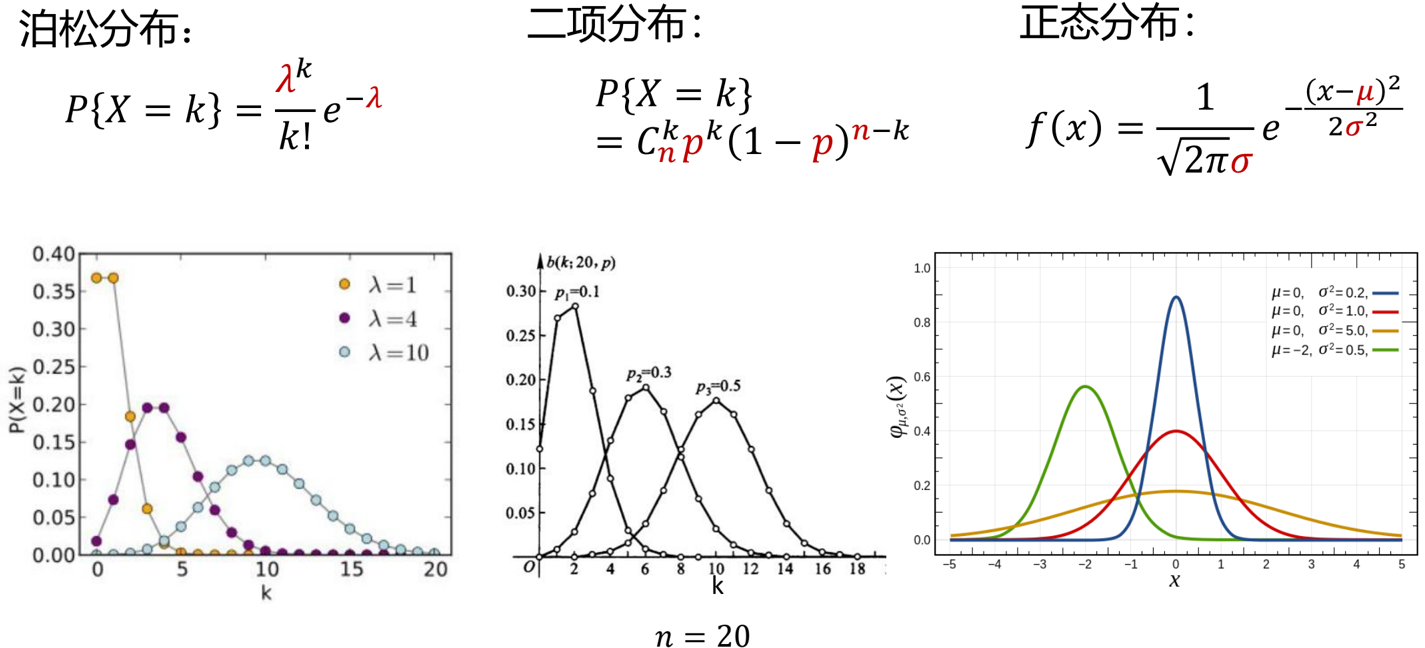
\includegraphics[width=0.5\textwidth]{figures/fig_dist_relationship_1.png}
    \caption{三种分布关系示意图}
    \label{fig:dist_relationship_1}
\end{figure}
\begin{itemize}[leftmargin=2em]
    \item \textbf{泊松分布}解决的是``在特定时间里发生 $k$ 个事件的概率''；
    \item \textbf{指数分布}解决的是``要等到一个随机事件发生，需要经历多久时间''；
    \item \textbf{$\Gamma$-分布}解决的是``要等到 $r$ 个随机事件都发生，需要经历多久时间''。
\end{itemize}
$\Gamma$-分布是泊松分布在正实数集上的连续化版本。泊松过程的事件间隔时间为指数分布；$\Gamma$-分布即为多个独立同分布的指数分布变量的和的分布。

\textbf{二项分布、泊松分布、正态分布的关系}：

\begin{figure}[htbp]
    \centering
    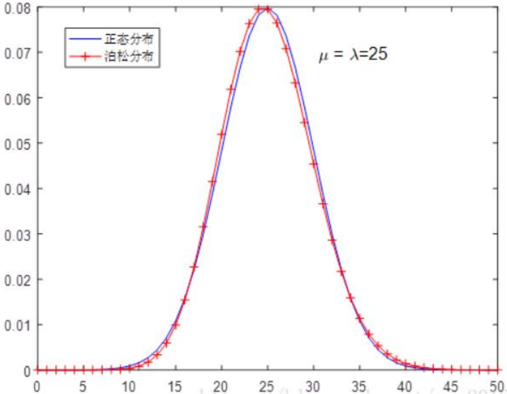
\includegraphics[width=0.5\textwidth]{figures/fig_dist_relationship_2.png}
    \caption{三种分布关系对比图（泊松、二项、正态）}
    \label{fig:dist_relationship_2}
\end{figure}
\begin{itemize}[leftmargin=2em]
    \item 二项分布当 $n$ 很大且 $np$ 不是很大时，近似泊松分布，$\lambda=np$；
    \item 二项分布当 $n$ 很大且 $np$ 也很大时，近似正态分布（$p$ 一般不能接近0或1）；
    \item 泊松分布当 $\lambda$ 很大时，也近似正态分布。
\end{itemize}

\textbf{扩展：多项分布（Multinomial Distribution）}：
多项分布是二项分布的扩展，它给出了 $K$-状态离散随机变量的概率分布：
\[
\mathrm{Mult}(m_1,m_2,\dots,m_K;\, n,\boldsymbol{p}) = \binom{n}{m_1\,m_2\,\dots\,m_K}\prod_{k=1}^{K}p_k^{m_k},
\]
其中 $\displaystyle\binom{n}{m_1\,m_2\,\dots\,m_K} = \frac{n!}{m_1!\,m_2!\,\cdots\,m_K!}$，$\sum_{k=1}^{K}p_k=1$。当 $K=2$ 时，即为二项分布。

\begin{example}[多项分布实例]
掷12个骰子，问骰子每面都出现两次的概率是多少？
\end{example}

\textbf{解}：$n=12$，$m_k=2$，$p_k=\dfrac{1}{6}\;(k=1,\dots,6)$。
\[
P(\text{骰子每面都出现两次}) = \binom{12}{2\,2\,2\,2\,2\,2}\prod_{k=1}^{6}\left(\frac{1}{6}\right)^2 = \frac{12!}{(2!)^6}\left(\frac{1}{6}\right)^{12} \approx 0.0034.
\]

\begin{figure}[htbp]
    \centering
    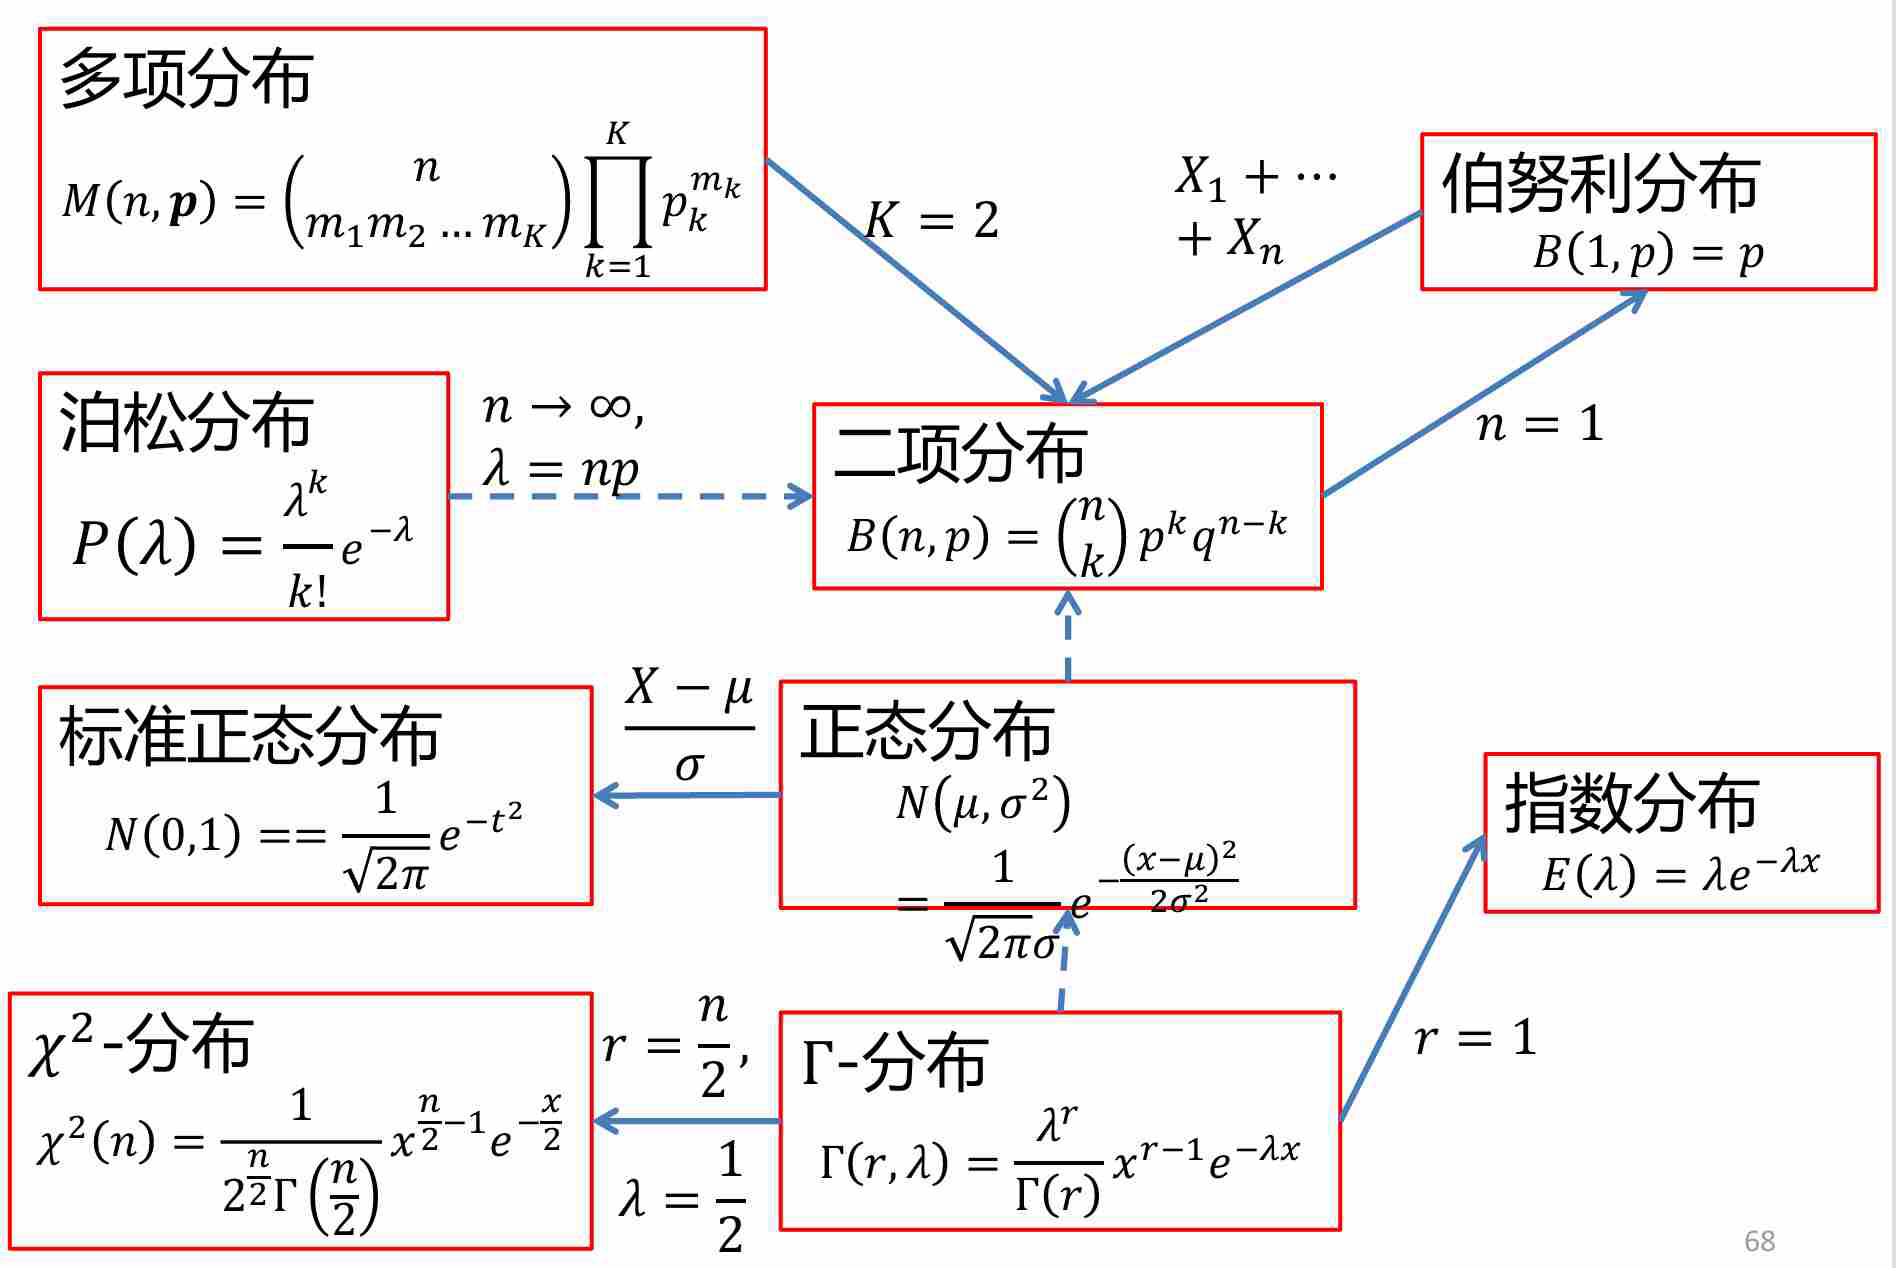
\includegraphics[width=0.6\textwidth]{figures/fig_all_distribution.png}
    \caption{常用概率分布及其关系总图}
    \label{fig:all_distribution}
\end{figure}

% ==================== 作业 ====================
\section*{作业}

\addcontentsline{toc}{section}{作业}

\subsection*{教材《概率论与数理统计》}
第二章（PP. 56--59）：\#1, \#3, \#4, \#8, \#12, \#16, \#21, \#25, \#29, \#31, \#32, \#35, \#37

\subsection*{教材《概率论及其应用》}
\begin{itemize}[leftmargin=2em]
    \item 6.10（PP. 130-131 / 139-140）：\#27, \#30, \#31
    \item 7.7（PP. 147-148 / 158-159）：\#1, \#9, \#10
\end{itemize}

\newpage

\chapter{多维随机变量及其分布}

\section{二维随机变量}

\subsection{二维随机变量的定义}

\begin{definition}[二维随机变量]
设 $E$ 是一个随机试验，它的样本空间是 $\Omega=\{e\}$，设 $X=X(e)$ 和 $Y=Y(e)$ 是定义在 $\Omega$ 上的随机变量。由它们构成的一个向量 $(X,Y)$，叫做二维随机向量，或二维随机变量。
\end{definition}

\begin{note}
多维随机变量本质上是从单个试验同时获得的多个随机变量。
\end{note}

\begin{figure}[htbp]
    \centering
    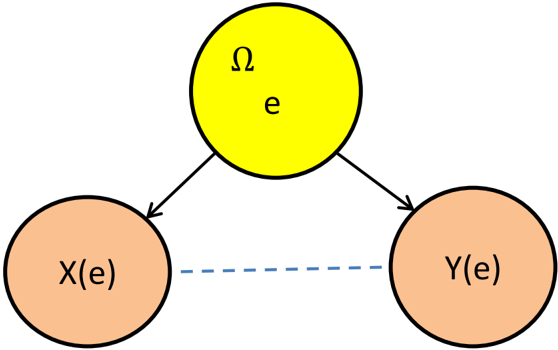
\includegraphics[width=0.5\textwidth]{figures/fig_2d_rv_mapping.png}
    \caption{样本空间到二维随机变量的映射示意图}
    \label{fig:2d_rv_mapping}
\end{figure}

研究多维随机变量的目的：
\begin{itemize}[leftmargin=2em]
    \item 随机变量之间存在某种关系（例如：身高与体重）；
    \item 依赖于随机变量的结果同时与多个随机变量相关（例如：健康状况的多个化验指标）。
\end{itemize}

应该把二维随机变量 $(X,Y)=(X(e),Y(e))\;(e\in\Omega)$ 看作一个整体，因为 $X$ 和 $Y$ 是有关联的。几何上 $(X,Y)$ 可以看作是平面坐标系上的点。

\begin{example}[成年男子的身体状况]
一个地区成年男子的身体状况。令 $X$ 表示身高，$Y$ 表示体重，则 $(X,Y)$ 就是一个二维随机变量。
\end{example}

\begin{example}[投掷飞镖游戏]
在投掷飞镖游戏中，令 $X$ 表示距靶心的水平距离，$Y$ 表示距靶心的垂直距离，则 $(X,Y)$ 就是一个二维随机变量。
\end{example}

\begin{example}[地区气候]
考察某地区的气候，令 $X$ 表示温度，$Y$ 表示气压，则 $(X,Y)$ 就是一个二维随机变量。
\end{example}

\subsection{二维随机变量的联合分布函数}

\begin{definition}[联合分布函数]
设 $(X,Y)$ 是二维随机变量，对任意实数 $x,y$，二元函数
\[
F(x,y)=P\{(X\leq x)\cap(Y\leq y)\}=P(X\leq x,Y\leq y)
\]
称为二维随机变量 $(X,Y)$ 的\textbf{联合分布}（Joint Distribution）函数，或简称为分布函数。
\end{definition}

\textbf{分布函数的几何意义}：$F(x,y)$ 在 $(x,y)$ 处的函数值就是随机点 $(X,Y)$ 落在以 $(x,y)$ 为右上角顶点的无穷矩形区域内的概率。

\begin{figure}[htbp]
    \centering
    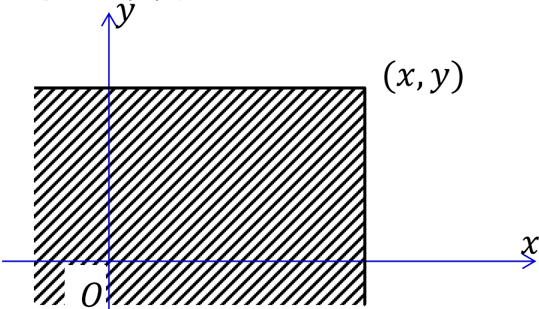
\includegraphics[width=0.5\textwidth]{figures/fig_joint_distribution_rectangle.png}
    \caption{联合分布函数的几何意义：无穷矩形区域}
    \label{fig:joint_distribution_rectangle}
\end{figure}

\textbf{一个基本公式}：若 $x_1<x_2,\;y_1<y_2$，则
\[
P(x_1<X\leq x_2,\;y_1<Y\leq y_2)=F(x_2,y_2)-F(x_2,y_1)-F(x_1,y_2)+F(x_1,y_1).
\]

\begin{figure}[htbp]
    \centering
    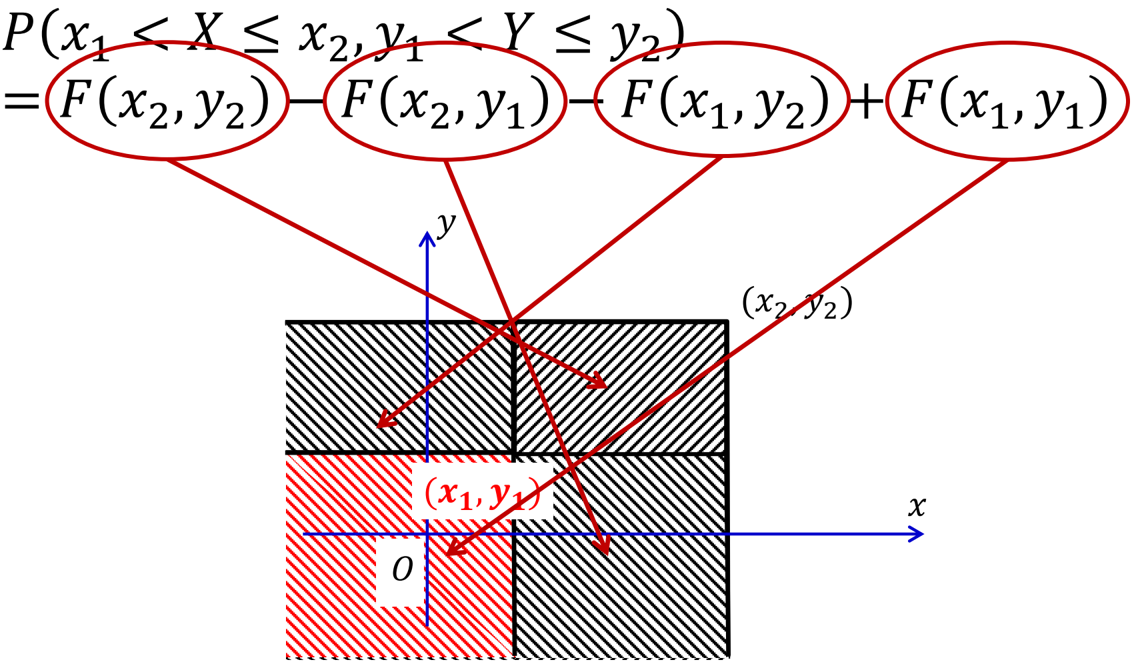
\includegraphics[width=0.5\textwidth]{figures/fig_rectangle_probability.png}
    \caption{矩形区域概率计算示意图}
    \label{fig:rectangle_probability}
\end{figure}

\subsection{分布函数的基本性质}

\begin{property}[分布函数的基本性质]
\begin{enumerate}[label=(\arabic*),leftmargin=2em]
    \item \textbf{单调性}：$F(x,y)$ 是变量 $x,y$ 的不减函数，即对于任意固定的 $y$，当 $x_1<x_2$ 时，
    \[
    F(x_1,y)\leq F(x_2,y).
    \]
    同样地，对于任意固定的 $x$，当 $y_1<y_2$ 时，
    \[
    F(x,y_1)\leq F(x,y_2).
    \]
    
    \item \textbf{有界性}：$0\leq F(x,y)\leq 1$，且对于任意固定的 $x$，
    \[
    F(x,-\infty)=0,
    \]
    对于任意固定的 $y$，
    \[
    F(-\infty,y)=0,\quad F(-\infty,-\infty)=0,\quad F(+\infty,+\infty)=1.
    \]
    
    \item \textbf{右连续}：
    \[
    F(x+0,y)=F(x,y),\quad F(x,y+0)=F(x,y).
    \]
    
    \item \textbf{非负性}：若 $x_1<x_2,\;y_1<y_2$，则
    \[
    F(x_2,y_2)+F(x_1,y_1)-F(x_2,y_1)-F(x_1,y_2)\geq 0.
    \]
\end{enumerate}
\end{property}

\begin{note}
任何二维随机变量的分布函数都满足这四条性质；任一具有这四条性质的二元函数均是二维随机变量的分布函数。
\end{note}

\subsection{二维离散型随机变量}

\begin{definition}[二维离散型随机变量]
若二维随机变量 $(X,Y)$ 的取值是有限个或可列无限多对时，则称 $(X,Y)$ 为\textbf{二维离散型随机变量}。

设 $(X,Y)$ 为二维离散型随机变量，$(X,Y)$ 的取值为 $(x_i,y_j)\;(i,j=1,2,\dots)$，并且记
\[
P(X=x_i,Y=y_j)=p_{ij},
\]
则称 $p_{ij}$ 为 $(X,Y)$ 的\textbf{分布律}或 $X$ 和 $Y$ 的\textbf{联合分布律}。
\end{definition}

二维离散型随机变量的联合分布律可以枚举，也可以用表格形式表现。

\begin{table}[htbp]
\centering
\caption{二维离散型随机变量的联合分布律}
\begin{tabular}{@{}cccccc@{}}
\toprule
$X\backslash Y$ & $y_1$ & $y_2$ & $\cdots$ & $y_j$ & $\cdots$ \\
\midrule
$x_1$ & $p_{11}$ & $p_{12}$ & $\cdots$ & $p_{1j}$ & $\cdots$ \\
$x_2$ & $p_{21}$ & $p_{22}$ & $\cdots$ & $p_{2j}$ & $\cdots$ \\
$\vdots$ & $\vdots$ & $\vdots$ & $\ddots$ & $\vdots$ & $\ddots$ \\
$x_i$ & $p_{i1}$ & $p_{i2}$ & $\cdots$ & $p_{ij}$ & $\cdots$ \\
$\vdots$ & $\vdots$ & $\vdots$ & $\ddots$ & $\vdots$ & $\ddots$ \\
\bottomrule
\end{tabular}
\end{table}

\begin{example}[例4：随机变量的联合分布律]
设随机变量 $X$ 在 $1,2,3,4$ 四个整数中等可能地取值，另一个随机变量 $Y$ 在 $1\sim X$ 之间等可能地取值，求 $(X,Y)$ 的分布律。
\end{example}

\textbf{解}：$X$ 的取值为 $1,2,3,4$，$Y$ 的取值为 $1,2,3,4$。由题意，
\[
P\{X=k\}=\frac{1}{4},\quad P\{Y=j\mid X=k\}=\frac{1}{k}\;(1\leq j\leq k).
\]
故
\[
P\{X=k,Y=j\}=P\{X=k\}P\{Y=j\mid X=k\}=\frac{1}{4k}\quad(1\leq j\leq k).
\]

\begin{table}[htbp]
\centering
\begin{tabular}{@{}ccccc@{}}
\toprule
$X\backslash Y$ & 1 & 2 & 3 & 4 \\
\midrule
1 & $\dfrac{1}{4}$ & $\dfrac{1}{8}$ & $\dfrac{1}{12}$ & $\dfrac{1}{16}$ \\[0.5em]
2 & 0 & $\dfrac{1}{8}$ & $\dfrac{1}{12}$ & $\dfrac{1}{16}$ \\[0.5em]
3 & 0 & 0 & $\dfrac{1}{12}$ & $\dfrac{1}{16}$ \\[0.5em]
4 & 0 & 0 & 0 & $\dfrac{1}{16}$ \\[0.5em]
\bottomrule
\end{tabular}
\end{table}

\begin{property}[二维离散型随机变量联合分布律的性质]
\begin{enumerate}[label=(\arabic*),leftmargin=2em]
    \item \textbf{非负性}：对任意 $i,j\;(i,j=1,2,\dots)$，
    \[
    p_{ij}=P\{X=x_i,Y=y_j\}\geq 0.
    \]
    \item \textbf{规范性}：
    \[
    \sum_{i,j}p_{ij}=1.
    \]
\end{enumerate}
\end{property}

\begin{example}[例5：抛硬币的联合分布]
将一枚均匀的硬币抛 $3$ 次，令
\[
X:\text{3次中出现正面的次数};\quad Y:\text{3次中正面出现次数与反面次数之差的绝对值}.
\]
给出 $(X,Y)$ 的联合分布律。
\end{example}

\textbf{解}：样本空间为
\[
\Omega=\{HHH,HHT,HTH,HTT,THH,THT,TTH,TTT\}.
\]
对应的 $X$ 的可能取值为 $0,1,2,3$，$Y$ 为 $1,3$。

\begin{table}[htbp]
\centering
\begin{tabular}{@{}ccccc@{}}
\toprule
$X\backslash Y$ & 0 & 1 & 2 & 3 \\
\midrule
1 & 0 & $\dfrac{3}{8}$ & $\dfrac{3}{8}$ & 0 \\[0.5em]
3 & $\dfrac{1}{8}$ & 0 & 0 & $\dfrac{1}{8}$ \\[0.5em]
\bottomrule
\end{tabular}
\end{table}

\textbf{二维离散型随机变量的联合分布函数}

类似一维情况，并考虑与连续情况的对应，引入分布函数。设二维离散型随机变量 $(X,Y)$ 的联合分布律为 $p_{ij}\;(i,j=1,2,\dots)$，则 $(X,Y)$ 的联合分布函数为
\[
F(x,y)=\sum_{x_i\leq x,\;y_j\leq y}p_{ij}.
\]

\subsection{二维连续型随机变量}

\begin{definition}[二维连续型随机变量]
对于二维随机变量 $(X,Y)$ 的分布函数 $F(x,y)$，如果存在非负可积函数 $f(x,y)$，使得对于任意的实数 $x,y$，有
\[
F(x,y)=\int_{-\infty}^{y}\int_{-\infty}^{x}f(u,v)\,du\,dv,
\]
则称 $(X,Y)$ 是\textbf{连续型的二维随机变量}，函数 $f(x,y)$ 称为二维随机变量 $(X,Y)$ 的\textbf{概率密度}，或称为 $X$ 和 $Y$ 的\textbf{联合概率密度}。
\end{definition}

\begin{property}[概率密度的性质]
\begin{enumerate}[label=(\arabic*),leftmargin=2em]
    \item \textbf{非负性}：$f(x,y)\geq 0$；
    \item \textbf{规范性}：
    \[
    \int_{-\infty}^{+\infty}\int_{-\infty}^{+\infty}f(u,v)\,du\,dv=F(+\infty,+\infty)=1;
    \]
    \item 设 $G$ 是 $xOy$ 平面上的一个区域，点 $(X,Y)$ 落在 $G$ 内的概率为
    \[
    P\{(X,Y)\in G\}=\iint_{(x,y)\in G}f(x,y)\,dx\,dy;
    \]
    \item 若 $f(x,y)$ 在点 $(x,y)$ 连续，则
    \[
    \frac{\partial^{2}F(x,y)}{\partial x\partial y}=f(x,y).
    \]
\end{enumerate}
\end{property}

\textbf{局部概率 $P\{(X,Y)\in G\}$ 的几何意义}

在几何上 $z=f(x,y)$ 表示空间的一个曲面，
\[
P\{(X,Y)\in G\}=\iint_{(x,y)\in G}f(x,y)\,dx\,dy
\]
即表示 $P\{(X,Y)\in G\}$ 的值等于以 $G$ 为底，以曲面 $z=f(x,y)$ 为顶的柱体体积。

\begin{figure}[htbp]
    \centering
    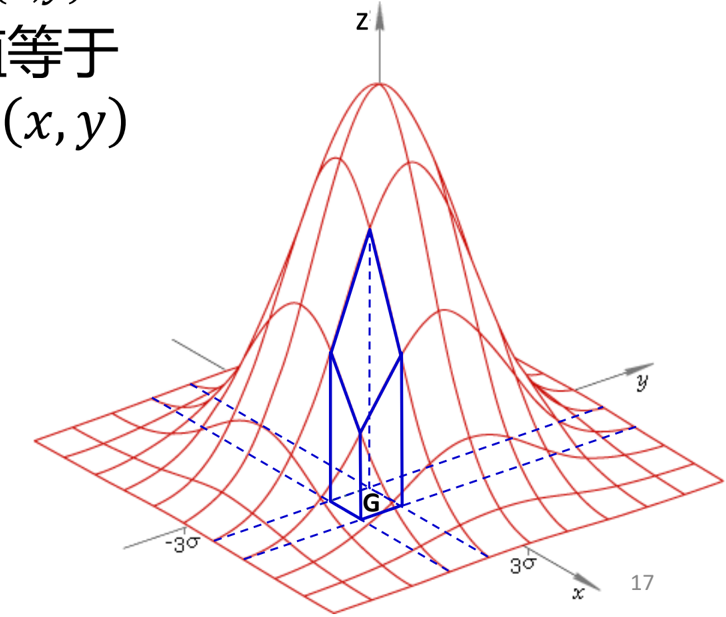
\includegraphics[width=0.5\textwidth]{figures/fig_2d_pdf_geometry.png}
    \caption{概率密度函数的几何意义：柱体体积}
    \label{fig:2d_pdf_geometry}
\end{figure}

\subsubsection{一些连续型二维随机变量}

\textbf{1. 二维均匀分布}

设 $D$ 是平面上的有界区域，其面积为 $A$，如果二维随机变量 $(X,Y)$ 的概率密度为
\[
f(x,y)=
\begin{cases}
\dfrac{1}{A}, & (x,y)\in D, \\[0.5em]
0, & (x,y)\notin D,
\end{cases}
\]
则称二维随机变量 $(X,Y)$ 服从区域 $D$ 上的\textbf{均匀分布}。

\begin{figure}[htbp]
    \centering
    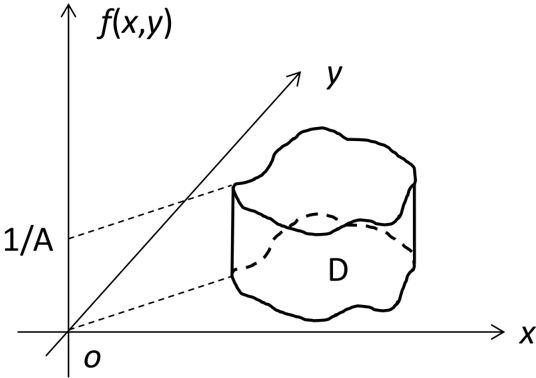
\includegraphics[width=0.5\textwidth]{figures/fig_2d_uniform.png}
    \caption{二维均匀分布概率密度示意图}
    \label{fig:2d_uniform}
\end{figure}

\textbf{2. 二维正态分布}

设二维随机变量 $(X,Y)$ 的密度函数为
\[
\begin{aligned}
f(x,y)&=\frac{1}{2\pi\sigma_{1}\sigma_{2}\sqrt{1-\rho^{2}}} \\
&\quad\cdot\exp\left\{-\frac{1}{2(1-\rho^{2})}\left[\frac{(x-\mu_{1})^{2}}{\sigma_{1}^{2}}-\frac{2\rho(x-\mu_{1})(y-\mu_{2})}{\sigma_{1}\sigma_{2}}+\frac{(y-\mu_{2})^{2}}{\sigma_{2}^{2}}\right]\right\},
\end{aligned}
\]
则称随机变量 $(X,Y)$ 服从参数为 $(\mu_{1},\mu_{2},\sigma_{1}^{2},\sigma_{2}^{2},\rho)$ 的\textbf{正态分布}，记为
\[
(X,Y)\sim N(\mu_{1},\mu_{2},\sigma_{1}^{2},\sigma_{2}^{2},\rho),
\]
其中 $-\infty<\mu_{i}<\infty,\;\sigma_{i}>0\;(i=1,2)$，$-1<\rho<1$。

\begin{figure}[htbp]
    \centering
    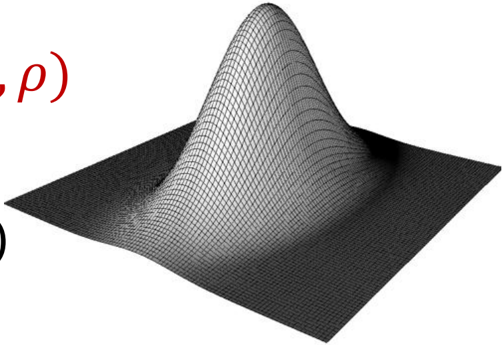
\includegraphics[width=0.5\textwidth]{figures/fig_2d_normal.png}
    \caption{二维正态分布概率密度示意图}
    \label{fig:2d_normal}
\end{figure}

\begin{example}[例6：确定常数与计算概率]
设二维随机变量 $(X,Y)$ 的密度函数为
\[
f(x,y)=
\begin{cases}
c\bigl(R-\sqrt{x^{2}+y^{2}}\bigr), & x^{2}+y^{2}<R^{2}, \\[0.3em]
0, & \text{其他},
\end{cases}
\]
(1) 求常数 $c$；(2) 求 $(X,Y)$ 落入圆 $x^{2}+y^{2}<r^{2}\;(0<r<R)$ 内的概率。
\end{example}

\textbf{解}：由概率归一化的特性有
\[
\int_{-\infty}^{+\infty}\int_{-\infty}^{+\infty}f(x,y)\,dx\,dy
=\iint_{x^{2}+y^{2}\leq R^{2}}c\bigl(R-\sqrt{x^{2}+y^{2}}\bigr)\,dx\,dy=1.
\]

变换到极坐标下 $x=\rho\cos\theta,\;y=\rho\sin\theta$，于是有
\[
\int_{0}^{2\pi}d\theta\int_{0}^{R}c(R-\rho)\rho\,d\rho=\frac{1}{3}\pi cR^{3}=1.
\]
故
\[
\boxed{c=\frac{3}{\pi R^{3}}}.
\]

(2) 类似地：
\[
P\bigl\{(X,Y)\in\{x^{2}+y^{2}<r^{2}\}\bigr\}
=\iint_{x^{2}+y^{2}<r^{2}}\frac{3}{\pi R^{3}}\bigl(R-\sqrt{x^{2}+y^{2}}\bigr)\,dx\,dy
=\frac{3r^{2}}{R^{2}}\left(1-\frac{2r}{3R}\right).
\]

\textbf{高斯分布的应用}

\begin{itemize}[leftmargin=2em]
    \item \textbf{高斯滤波}：左：原图；中：均值滤波；右：高斯滤波。
    \item \textbf{高斯混合模型聚类}（Gaussian Mixture Models）：左：输入数据；右：聚类结果。
    \item \textbf{3D Gaussian Splatting}。
\end{itemize}

\begin{figure}[htbp]
    \centering
    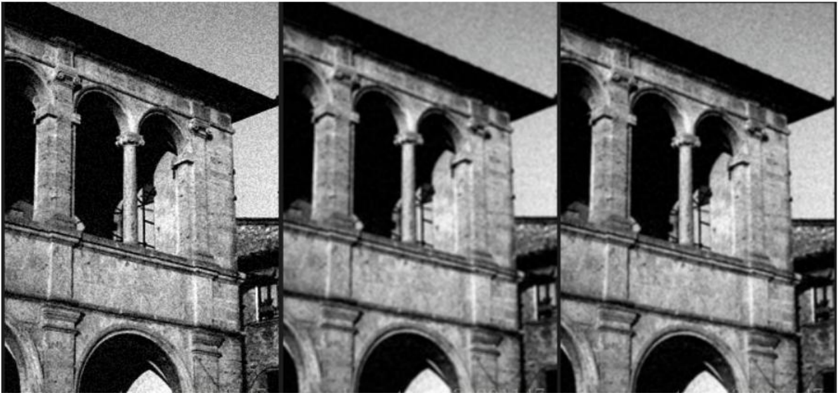
\includegraphics[width=0.6\textwidth]{figures/fig_gaussian_filter.png}
    \caption{高斯滤波效果对比图}
    \label{fig:gaussian_filter}
\end{figure}

\begin{figure}[htbp]
    \centering
    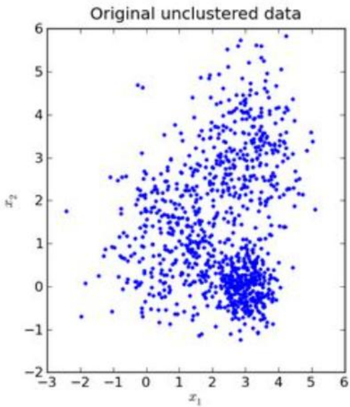
\includegraphics[width=0.6\textwidth]{figures/fig_gmm_clustering.png}
    \caption{高斯混合模型聚类示意图}
    \label{fig:gmm_clustering}
\end{figure}

\begin{figure}[htbp]
    \centering
    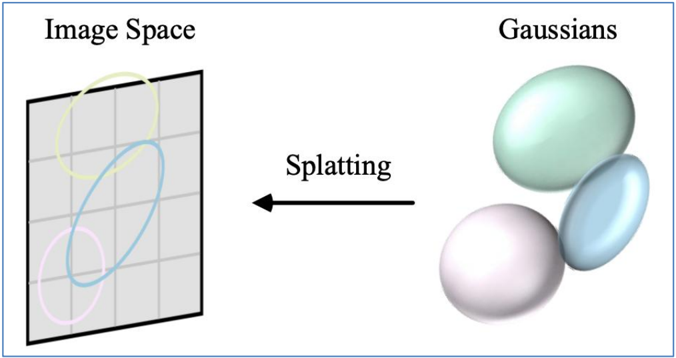
\includegraphics[width=0.6\textwidth]{figures/fig_3d_gaussian_splatting.png}
    \caption{3D Gaussian Splatting 示意图}
    \label{fig:3d_gaussian_splatting}
\end{figure}

\subsection{从二维到\texorpdfstring{$n$}{n}维}

\begin{definition}[$n$维随机变量]
设 $E$ 是一个随机试验，它的样本空间是 $\Omega=\{e\}$，设 $X_{i}=X_{i}(e)\;(e\in\Omega,\;i=1,2,\dots,n)$ 是定义在 $\Omega$ 上的 $n$ 个随机变量。由它们构成的一个向量 $(X_{1},X_{2},\dots,X_{n})$，叫做样本空间 $\Omega$ 上的 $n$ 维随机向量，或 $n$ 维随机变量。
\end{definition}

\textbf{$n$ 维随机变量的分布函数}

设 $(X_{1},X_{2},\dots,X_{n})$ 是一个 $n$ 维随机变量，则对于任一 $n$ 维实数组 $(x_{1},x_{2},\dots,x_{n})$，
\[
F(x_{1},x_{2},\dots,x_{n})=P\{X_{1}\leq x_{1},X_{2}\leq x_{2},\dots,X_{n}\leq x_{n}\},
\]
称此函数为 $n$ 维随机变量的分布函数。

\section{边缘分布}

\subsection{边缘分布的定义}

设 $(X,Y)$ 为二维随机向量，其分布函数为 $F(x,y)$。其中分量 $X$ 或 $Y$ 是一维随机变量，相应的存在一维分布，分别记为 $F_{X}(x)$ 和 $F_{Y}(y)$，依次称 $F_{X}(x),F_{Y}(y)$ 为 $(X,Y)$ 关于 $X$ 和关于 $Y$ 的\textbf{边缘分布函数}。

\begin{note}
边缘分布又翻译为``边际分布''或``边沿分布''。
\end{note}

\subsection{边缘分布函数}

利用联合分布函数获得边缘分布函数。

设二维随机变量 $(X,Y)$ 的分布函数为 $F(x,y)$，则分量 $X$ 的边缘分布函数为
\[
F_{X}(x)=P\{X\leq x\}=P\{X\leq x,Y<+\infty\}=\lim_{y\to+\infty}F(x,y)=F(x,+\infty).
\]
类似地，对分量 $Y$ 的边缘分布函数为
\[
F_{Y}(y)=P\{Y\leq y\}=P\{Y\leq y,X<+\infty\}=\lim_{x\to+\infty}F(x,y)=F(+\infty,y).
\]

\begin{note}
上述方法适用于离散和连续情形。
\end{note}

\begin{example}[例7：确定常数并求边缘分布]
设二维随机变量 $(X,Y)$ 的联合分布函数为
\[
F(x,y)=A\left(B+\arctan\frac{x}{2}\right)\left(C+\arctan\frac{y}{5}\right),\quad (-\infty<x,y<+\infty)
\]
求常数 $A,B,C$ 以及边缘分布函数。
\end{example}

\textbf{解}：由分布函数性质有
\begin{align*}
F(+\infty,+\infty)&=A\left(B+\frac{\pi}{2}\right)\left(C+\frac{\pi}{2}\right)=1, \tag{1}\\
F(-\infty,+\infty)&=A\left(B-\frac{\pi}{2}\right)\left(C+\frac{\pi}{2}\right)=0, \tag{2}\\
F(+\infty,-\infty)&=A\left(B+\frac{\pi}{2}\right)\left(C-\frac{\pi}{2}\right)=0. \tag{3}
\end{align*}
由 (2),(3) 得 $B=\dfrac{\pi}{2},\;C=\dfrac{\pi}{2}$，代入 (1)，有
\[
\boxed{A=\frac{1}{\pi^{2}}}.
\]

于是
\[
F_{X}(x)=\lim_{y\to+\infty}F(x,y)=\frac{1}{\pi^{2}}\left(\frac{\pi}{2}+\arctan\frac{x}{2}\right)\left(\frac{\pi}{2}+\frac{\pi}{2}\right)=\frac{1}{\pi}\left(\frac{\pi}{2}+\arctan\frac{x}{2}\right).
\]
类似地，
\[
F_{Y}(y)=\lim_{x\to+\infty}F(x,y)=\frac{1}{\pi}\left(\frac{\pi}{2}+\arctan\frac{y}{5}\right).
\]

\subsection{边缘分布律}

利用联合分布律求边缘分布律。

已知二维离散型随机变量 $(X,Y)$ 的联合分布律为
\[
p_{ij}=P\{X=x_{i},Y=y_{j}\}\quad(i,j=1,2,\dots)
\]
则随机变量 $X$ 的边缘分布律为
\[
p_{i\cdot}=P\{X=x_{i}\}=\sum_{j}P\{X=x_{i},Y=y_{j}\}=\sum_{j}p_{ij}\quad(i=1,2,\dots).
\]
类似地，随机变量 $Y$ 的边缘分布律为
\[
p_{\cdot j}=P\{Y=y_{j}\}=\sum_{i}p_{ij}\quad(j=1,2,\dots).
\]

\begin{figure}[htbp]
    \centering
    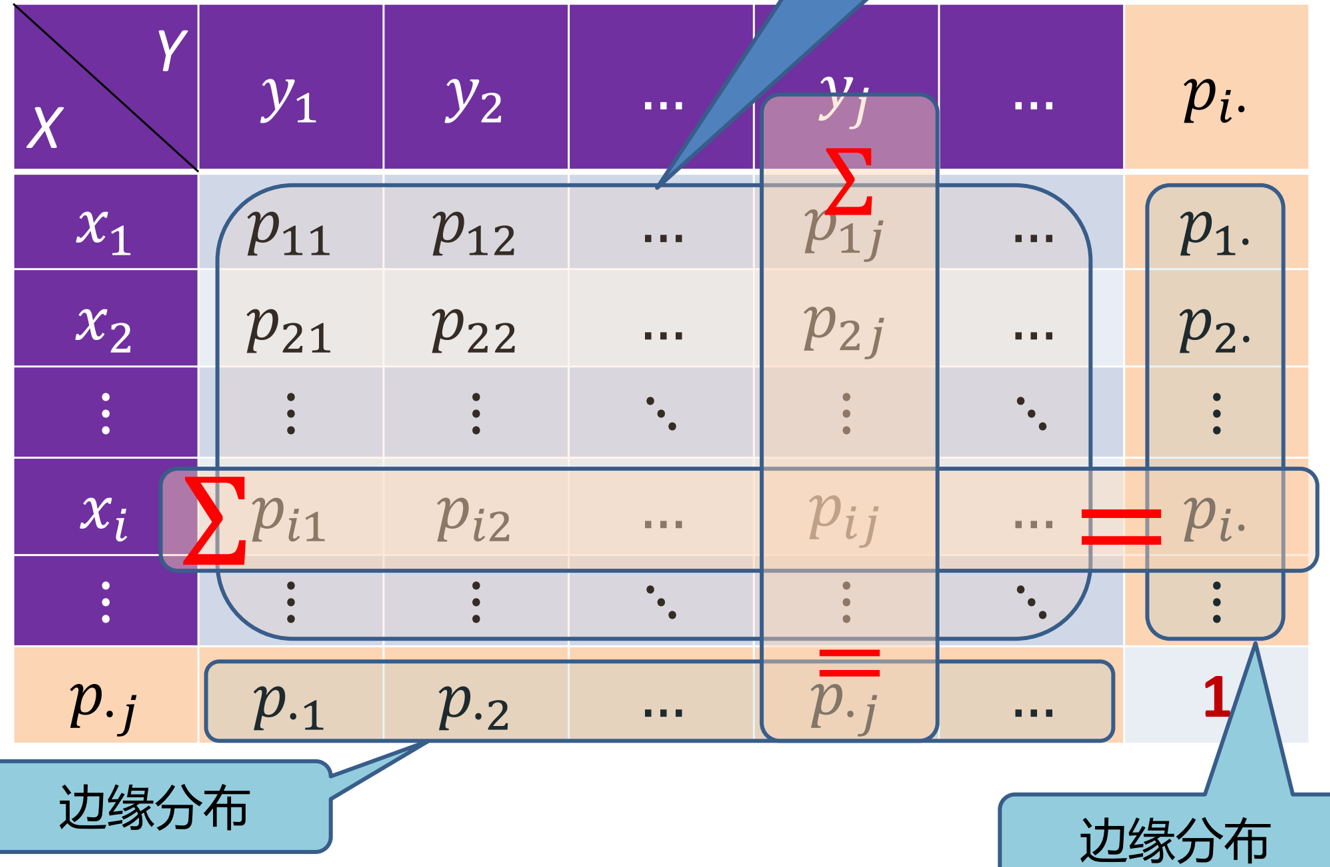
\includegraphics[width=0.8\textwidth]{figures/fig_marginal_distribution_table.png}
    \caption{联合分布律与边缘分布示意图}
    \label{fig:marginal_distribution_table}
\end{figure}

\begin{example}[例8：鸟类寄生虫的边缘分布]
下表中给出了两种不同类型的鸟（A和B）寄生了两种类型的寄生虫——虱子和螨虫。由于这两种寄生虫相当大，鸟身上有同类寄生虫的数量不会超过两个。对每一种鸟身上具有的特定寄生虫数量的概率进行了统计。例如，在一只鸟身上有一只螨虫和两支虱子的概率为 $0.09$，有两只螨虫和一只虱子的概率为 $0.06$。求两类鸟的边缘分布。
\end{example}

\begin{table}[htbp]
\centering
\caption{Bird A 的联合分布律与边缘分布}
\begin{tabular}{@{}ccccc@{}}
\toprule
虱子\textbackslash 螨虫 & 0 & 1 & 2 & 边缘 \\
\midrule
0 & 0.20 & 0.15 & 0.15 & 0.5 \\
1 & 0.12 & 0.09 & 0.09 & 0.3 \\
2 & 0.08 & 0.06 & 0.06 & 0.2 \\
\midrule
边缘 & 0.4 & 0.3 & 0.3 & \\
\bottomrule
\end{tabular}
\end{table}

\begin{table}[htbp]
\centering
\caption{Bird B 的联合分布律与边缘分布}
\begin{tabular}{@{}ccccc@{}}
\toprule
虱子\textbackslash 螨虫 & 0 & 1 & 2 & 边缘 \\
\midrule
0 & 0.33 & 0.08 & 0.09 & 0.5 \\
1 & 0.05 & 0.13 & 0.12 & 0.3 \\
2 & 0.02 & 0.09 & 0.09 & 0.2 \\
\midrule
边缘 & 0.4 & 0.3 & 0.3 & \\
\bottomrule
\end{tabular}
\end{table}

\textbf{解}：为求出每类鸟身上虱子的数量的边缘概率分布，将每一列中的数字相加。例如 A 类鸟身上有一只虱子的概率为
\[
0.15+0.09+0.06=0.3.
\]
类似的，螨虫数量的边缘分布为每一行中的数字相加，例如 B 类鸟身上有两只螨虫的概率为
\[
0.02+0.09+0.09=0.2.
\]

\begin{note}
尽管两类鸟身上昆虫的分布不同，但边缘分布是一样的，也就是从边缘分布不能唯一确定联合分布。从联合分布律求边缘分布律仅适用于离散分布。
\end{note}

\subsection{边缘密度函数}

利用联合概率密度函数求边缘密度函数。

已知二维连续型随机变量 $(X,Y)$，已知其联合分布密度函数为 $f(x,y)$，则随机变量 $X$ 的边缘分布为
\[
F_{X}(x)=P\{X\leq x\}=F(x,+\infty)=\int_{-\infty}^{x}\int_{-\infty}^{+\infty}f(x,y)\,dy\,dx=\int_{-\infty}^{x}f_{X}(x)\,dx.
\]
于是，
\[
\boxed{f_{X}(x)=\int_{-\infty}^{+\infty}f(x,y)\,dy}.
\]
类似地，
\[
\boxed{f_{Y}(y)=\int_{-\infty}^{+\infty}f(x,y)\,dx}.
\]

\begin{example}[例9：均匀分布的边缘密度]
设平面区域 $D$ 是由抛物线 $y=x^{2}$ 及直线 $y=x$ 所围成，随机变量 $(X,Y)$ 服从区域 $D$ 上的均匀分布，试求随机变量 $(X,Y)$ 的联合密度函数及 $X,Y$ 各自的边缘密度函数。
\end{example}

\textbf{解}：区域 $D$ 的面积为
\[
S=\int_{0}^{1}\int_{x^{2}}^{x}dy\,dx=\int_{0}^{1}(x-x^{2})\,dx=\left[\frac{x^{2}}{2}-\frac{x^{3}}{3}\right]_{0}^{1}=\frac{1}{6}.
\]
于是 $(X,Y)$ 的联合概率密度函数为
\[
f(x,y)=
\begin{cases}
6, & (x,y)\in D, \\[0.3em]
0, & (x,y)\notin D.
\end{cases}
\]

\begin{figure}[htbp]
    \centering
    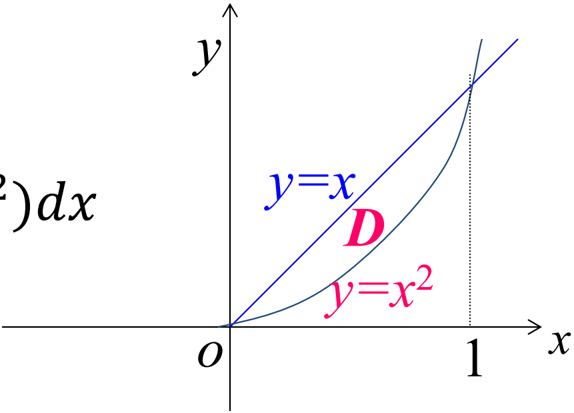
\includegraphics[width=0.5\textwidth]{figures/fig_region_D.png}
    \caption{区域 $D$ 由 $y=x^{2}$ 与 $y=x$ 围成}
    \label{fig:region_D}
\end{figure}

求 $X$ 的边缘密度函数：
\[
f_{X}(x)=\int_{x^{2}}^{x}6\,dy=6(x-x^{2}),\quad 0\leq x\leq 1.
\]
于是
\[
f_{X}(x)=
\begin{cases}
6(x-x^{2}), & 0\leq x\leq 1, \\[0.3em]
0, & \text{其他}.
\end{cases}
\]

类似地，求 $Y$ 的边缘密度函数：
\[
f_{Y}(y)=\int_{y}^{\sqrt{y}}6\,dx=6(\sqrt{y}-y),\quad 0\leq y\leq 1.
\]
于是
\[
f_{Y}(y)=
\begin{cases}
6(\sqrt{y}-y), & 0\leq y\leq 1, \\[0.3em]
0, & \text{其他}.
\end{cases}
\]

\begin{example}[例10：二维正态分布的边缘分布]
设二维随机变量 $(X,Y)$ 服从参数为 $(\mu_{1},\mu_{2},\sigma_{1}^{2},\sigma_{2}^{2},\rho)$ 的正态分布，即密度函数为
\[
\begin{aligned}
f(x,y)&=\frac{1}{2\pi\sigma_{1}\sigma_{2}\sqrt{1-\rho^{2}}} \\
&\quad\cdot\exp\left\{-\frac{1}{2(1-\rho^{2})}\left[\frac{(x-\mu_{1})^{2}}{\sigma_{1}^{2}}-\frac{2\rho(x-\mu_{1})(y-\mu_{2})}{\sigma_{1}\sigma_{2}}+\frac{(y-\mu_{2})^{2}}{\sigma_{2}^{2}}\right]\right\},
\end{aligned}
\]
给出 $X$ 和 $Y$ 的边缘分布。
\end{example}

\textbf{解}：先求 $Y$ 的边缘密度函数
\[
f_{Y}(y)=\int_{-\infty}^{+\infty}f(x,y)\,dx.
\]
记 $C=\dfrac{1}{2\pi\sigma_{1}\sigma_{2}\sqrt{1-\rho^{2}}}$，则
\begin{align*}
f_{Y}(y)&=C\int_{-\infty}^{\infty}\exp\left\{-\frac{1}{2(1-\rho^{2})}\left[\frac{(x-\mu_{1})^{2}}{\sigma_{1}^{2}}-\frac{2\rho(x-\mu_{1})(y-\mu_{2})}{\sigma_{1}\sigma_{2}}+\frac{(y-\mu_{2})^{2}}{\sigma_{2}^{2}}\right]\right\}dx \\
&=C\exp\left\{-\frac{(y-\mu_{2})^{2}}{2(1-\rho^{2})\sigma_{2}^{2}}\right\}\int_{-\infty}^{\infty}\exp\left\{-\frac{1}{2(1-\rho^{2})}\left[\frac{(x-\mu_{1})^{2}}{\sigma_{1}^{2}}-\frac{2\rho(x-\mu_{1})(y-\mu_{2})}{\sigma_{1}\sigma_{2}}\right]\right\}dx.
\end{align*}
对指数部分配方，令
\[
x'=\frac{x-\mu_{1}}{\sigma_{1}}-\frac{\rho(y-\mu_{2})}{\sigma_{2}},
\]
则
\[
f_{Y}(y)=C\sigma_{1}\exp\left\{-\frac{(y-\mu_{2})^{2}}{2\sigma_{2}^{2}}\right\}\int_{-\infty}^{\infty}\exp\left\{-\frac{1}{2(1-\rho^{2})}x'^{2}\right\}dx'.
\]
注意到
\[
\int_{-\infty}^{\infty}\exp\left\{-\frac{1}{2(1-\rho^{2})}x'^{2}\right\}dx'=\sqrt{2(1-\rho^{2})\pi},
\]
于是
\[
f_{Y}(y)=C\sigma_{1}\exp\left\{-\frac{(y-\mu_{2})^{2}}{2\sigma_{2}^{2}}\right\}\sqrt{2(1-\rho^{2})\pi}
=\frac{1}{\sqrt{2\pi}\sigma_{2}}\exp\left\{-\frac{(y-\mu_{2})^{2}}{2\sigma_{2}^{2}}\right\}.
\]

类似地，
\[
f_{X}(x)=\frac{1}{\sqrt{2\pi}\sigma_{1}}\exp\left\{-\frac{(x-\mu_{1})^{2}}{2\sigma_{1}^{2}}\right\}.
\]

于是
\[
X\sim N(\mu_{1},\sigma_{1}^{2}),\qquad Y\sim N(\mu_{2},\sigma_{2}^{2}).
\]

\begin{note}[几点有关的结论]
\begin{enumerate}[leftmargin=2em]
    \item 二维正态分布的边缘分布还是正态分布，且与相关系数 $\rho$ 无关；
    \item 相同的两个边缘分布不能唯一决定联合分布，这时 $\rho$ 可以不同；
    \item 甚至两个正态的边缘可以来自一个非正态的二维分布。
\end{enumerate}
\end{note}

关于第三点的一个例子：
\[
f(x,y)=\frac{1}{2\pi}\exp\left\{-\frac{x^{2}+y^{2}}{2}\right\}(1+\sin x\sin y),\quad -\infty<x,y<+\infty,
\]
其边缘分布为 $X\sim N(0,1)$，$Y\sim N(0,1)$。

\subsection{从二维到\texorpdfstring{$n$}{n}维}

设 $(X_{1},X_{2},\dots,X_{n})$ 是一个 $n$ 维随机变量，若存在非负函数 $f(x_{1},x_{2},\dots,x_{n})$，使得对任意实数 $x_{1},x_{2},\dots,x_{n}$ 有
\[
F(x_{1},x_{2},\dots,x_{n})=\int_{-\infty}^{x_{n}}\cdots\int_{-\infty}^{x_{2}}\int_{-\infty}^{x_{1}}f(x_{1},x_{2},\dots,x_{n})\,dx_{1}\,dx_{2}\dots dx_{n},
\]
称 $f(x_{1},x_{2},\dots,x_{n})$ 为 $n$ 维随机变量 $(X_{1},X_{2},\dots,X_{n})$ 的分布密度函数。

相应地，一个 $k$-维分布函数的例子为
\[
F_{(X_{1},X_{2},\dots,X_{k})}(x_{1},x_{2},\dots,x_{k})=F(x_{1},x_{2},\dots,x_{k},+\infty,\dots,+\infty).
\]
一个 $k$-维分布密度函数的例子为
\[
\begin{aligned}
&f_{(X_{1},X_{2},\dots,X_{k})}(x_{1},x_{2},\dots,x_{k}) \\
&\qquad=\int_{-\infty}^{+\infty}\cdots\int_{-\infty}^{+\infty}\int_{-\infty}^{+\infty}f(\dots,x_{k+1},x_{k+2},\dots,x_{n})\,dx_{k+1}\,dx_{k+2}\dots dx_{n}.
\end{aligned}
\]

\section*{作业}

\addcontentsline{toc}{section}{作业}

教材《概率论与数理统计》第三章（pp.~84--86）：\#1, \#5, \#6, \#9.

\section{两个随机变量的函数的分布}

\subsection{回顾随机变量函数的分布}

上一章中讨论了单个随机变量的函数的分布。一般方法：若 $X\sim f(x)$，$-\infty<x<+\infty$，$Y=g(X)$ 为随机变量 $X$ 的函数，则可先求 $Y$ 的分布函数
\[
F_{Y}(y)=P\{Y\leq y\}=P\{g(X)\leq y\}=\int_{g(x)\leq y}f(x)\,dx,
\]
进一步获得 $Y$ 的概率密度函数
\[
f_{Y}(y)=\frac{dF_{Y}(y)}{dy}.
\]

\subsection{二元随机变量的函数的分布}

若 $(X,Y)\sim f(x,y)$，$-\infty<x,y<+\infty$，$Z=g(X,Y)$ 为随机变量 $(X,Y)$ 的函数，则可先求 $Z$ 的分布函数
\[
F_{Z}(z)=P\{Z\leq z\}=P\{g(X,Y)\leq z\}=\iint_{g(x,y)\leq z}f(x,y)\,dx\,dy.
\]
进一步获得 $Z$ 的概率密度函数
\[
f_{Z}(z)=\frac{dF_{Z}(z)}{dz}.
\]

本节考虑几种特殊的二元函数：
\begin{itemize}[leftmargin=2em]
    \item $Z=X+Y$；
    \item $Z=Y/X$ 和 $Z=XY$；
    \item $Z=\max\{X,Y\}$ 和 $Z=\min\{X,Y\}$。
\end{itemize}

\subsection{几个常用二维随机变量函数的分布}

\subsubsection{\texorpdfstring{$Z=X+Y$}{Z=X+Y} 的分布}

设 $(X,Y)$ 的概率密度为 $f(x,y)$，则 $Z=X+Y$ 的分布函数为
\[
F_{Z}(z)=P\{Z\leq z\}=\iint_{x+y\leq z}f(x,y)\,dx\,dy.
\]

\begin{figure}[htbp]
    \centering
    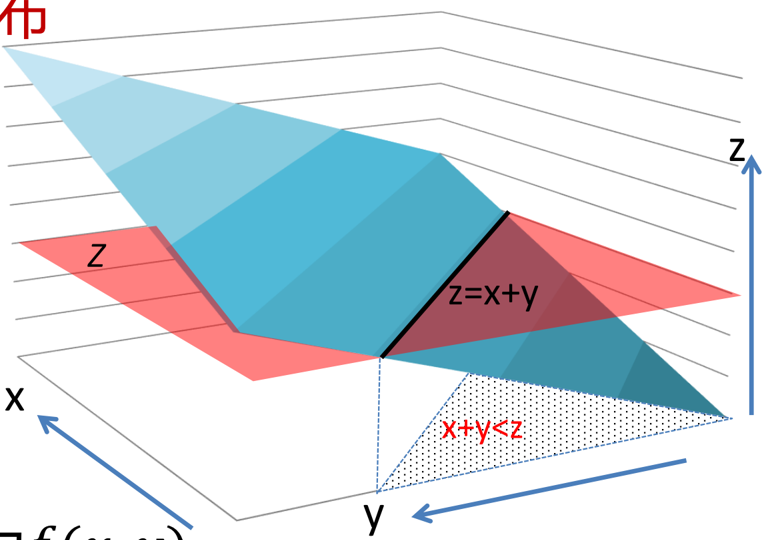
\includegraphics[width=0.6\textwidth]{figures/fig_sum_distribution_3d.png}
    \caption{$Z=X+Y$ 的分布：积分区域 $x+y<z$}
    \label{fig:sum_distribution_3d}
\end{figure}

将重积分化为累次积分：
\[
F_{Z}(z)=\int_{-\infty}^{\infty}\left[\int_{-\infty}^{z-y}f(x,y)\,dx\right]dy.
\]
固定 $y,z$，作变量代换，令 $x=u-y$，得
\[
\int_{-\infty}^{z-y}f(x,y)\,dx=\int_{-\infty}^{z}f(u-y,y)\,du.
\]
于是
\[
F_{Z}(z)=\int_{-\infty}^{\infty}\int_{-\infty}^{z}f(u-y,y)\,du\,dy
=\int_{-\infty}^{z}\left[\int_{-\infty}^{\infty}f(u-y,y)\,dy\right]du.
\]
由概率密度的定义，即得到 $Z$ 的概率密度为
\[
\boxed{f_{Z}(z)=\int_{-\infty}^{\infty}f(z-y,y)\,dy}. \tag{*1}
\]
由 $X,Y$ 的对称性，有
\[
\boxed{f_{Z}(z)=\int_{-\infty}^{\infty}f(x,z-x)\,dx}. \tag{*2}
\]
以上两式是两个随机变量和的概率密度的一般公式。

\textbf{卷积公式}

当 $X$ 和 $Y$ 相互独立时，则 $(*1)$ 和 $(*2)$ 式分别化为
\[
\boxed{f_{Z}(z)=\int_{-\infty}^{\infty}f_{X}(z-y)f_{Y}(y)\,dy}
\]
和
\[
\boxed{f_{Z}(z)=\int_{-\infty}^{\infty}f_{X}(x)f_{Y}(z-x)\,dx}.
\]
这两个公式称为\textbf{卷积公式}，记作 $f_{X}*f_{Y}$。

\begin{example}[例1：正态分布的可加性]
设随机变量 $X$ 与 $Y$ 独立且均服从标准正态分布，求 $Z=X+Y$ 的概率密度函数。
\end{example}

\textbf{解}：由于
\[
f_{X}(x)=\frac{1}{\sqrt{2\pi}}e^{-x^{2}/2},\quad
f_{Y}(y)=\frac{1}{\sqrt{2\pi}}e^{-y^{2}/2},\quad
(-\infty<x,y<\infty)
\]
于是 $Z$ 的密度函数为
\begin{align*}
f_{Z}(z)&=\int_{-\infty}^{\infty}f_{X}(z-y)f_{Y}(y)\,dy
=\frac{1}{2\pi}\int_{-\infty}^{\infty}e^{-\frac{(z-y)^{2}+y^{2}}{2}}\,dy\\
&=\frac{1}{2\pi}e^{-\frac{z^{2}}{4}}\int_{-\infty}^{\infty}e^{-\left(y-\frac{z}{2}\right)^{2}}\,dy
=\frac{1}{2\pi}e^{-\frac{z^{2}}{4}}\cdot\sqrt{\pi}
=\frac{1}{2\sqrt{\pi}}e^{-\frac{z^{2}}{4}}.
\end{align*}
于是 $Z\sim N(0,2)$。

\begin{note}[更为一般的结论]
有限个相互独立的正态随机变量的线性组合仍然服从正态分布，即

若 $X_{i}\sim N(\mu_{i},\sigma_{i}^{2})\;(i=1,2,\dots,n)$，且相互独立，$Z=\sum_{i=1}^{n}X_{i}$，则
\[
\boxed{Z\sim N\left(\sum_{i=1}^{n}\mu_{i},\;\sum_{i=1}^{n}\sigma_{i}^{2}\right)}.
\]
\end{note}

\begin{example}[例2：串联电阻]
在一简单电路中，两个电阻 $R_{1}$ 和 $R_{2}$ 串联连接，设 $R_{1}$ 和 $R_{2}$ 相互独立，它们的概率密度函数均为
\[
f(x)=
\begin{cases}
\dfrac{10-x}{50}, & 0\leq x\leq 10,\\[0.5em]
0, & \text{其他},
\end{cases}
\]
求总电阻 $R=R_{1}+R_{2}$ 的概率密度。
\end{example}

\textbf{解}：$R$ 的概率密度为
\[
f_{R}(z)=\int_{-\infty}^{\infty}f(x)f(z-x)\,dx.
\]
非零的积分区域如右图中阴影区域，即
\[
\begin{cases}
0\leq x\leq 10,\\[0.3em]
0\leq z-x\leq 10.
\end{cases}
\]

\begin{figure}[htbp]
    \centering
    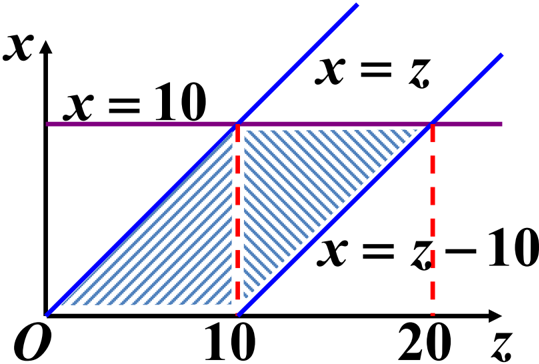
\includegraphics[width=0.5\textwidth]{figures/fig_resistor_convolution_region.png}
    \caption{卷积非零积分区域示意图}
    \label{fig:resistor_convolution_region}
\end{figure}

于是
\[
f_{R}(z)=
\begin{cases}
\displaystyle\int_{0}^{z}f(x)f(z-x)\,dx, & 0\leq z<10,\\[1em]
\displaystyle\int_{z-10}^{10}f(x)f(z-x)\,dx, & 10\leq z<20,\\[1em]
0, & \text{其他}.
\end{cases}
\]
代入 $f(x)=\dfrac{10-x}{50}$ 计算得
\[
f_{R}(z)=
\begin{cases}
\dfrac{600z-60z^{2}+z^{3}}{15000}, & 0\leq z<10,\\[0.8em]
\dfrac{(20-z)^{3}}{15000}, & 10\leq z<20,\\[0.8em]
0, & \text{其他}.
\end{cases}
\]

\begin{example}[例3：均匀分布与指数分布之和]
设随机变量 $X$ 与 $Y$ 相互独立，$X$ 服从区间 $(0,1)$ 上的均匀分布，$Y$ 服从 $\lambda=1$ 的指数分布，令 $Z=X+Y$，试求随机变量 $Z$ 的密度函数。
\end{example}

\textbf{解}：由题意：
\[
f_{X}(x)=
\begin{cases}
1, & 0<x<1,\\[0.3em]
0, & \text{其他},
\end{cases}
\qquad
f_{Y}(y)=
\begin{cases}
e^{-y}, & y>0,\\[0.3em]
0, & y\leq 0.
\end{cases}
\]
于是
\[
f_{X}(x)f_{Y}(z-x)=
\begin{cases}
e^{-(z-x)}, & 0<x<1,\;z-x>0,\\[0.3em]
0, & \text{其他}.
\end{cases}
\]

\begin{figure}[htbp]
    \centering
    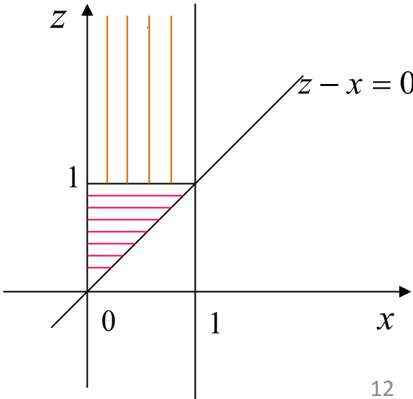
\includegraphics[width=0.5\textwidth]{figures/fig_uniform_exponential_sum.png}
    \caption{$Z=X+Y$ 的积分域示意图}
    \label{fig:uniform_exponential_sum}
\end{figure}

注意积分域如右图，于是分情况讨论：
\begin{enumerate}[label=(\arabic*),leftmargin=2em]
    \item 若 $z\leq 0$，则 $f_{Z}(z)=0$；
    \item 若 $0<z\leq 1$，
    \[
    f_{Z}(z)=\int_{0}^{z}e^{-(z-x)}\,dx=e^{-z}\int_{0}^{z}e^{x}\,dx=1-e^{-z};
    \]
    \item 若 $z>1$，
    \[
    f_{Z}(z)=\int_{0}^{1}e^{-(z-x)}\,dx=e^{-z}\int_{0}^{1}e^{x}\,dx=e^{-z+1}-e^{-z}.
    \]
\end{enumerate}

于是，$(0,1)$ 上均匀分布与 $\lambda=1$ 的指数分布的和函数的密度函数为
\[
f_{Z}(z)=
\begin{cases}
0, & z\leq 0,\\[0.3em]
1-e^{-z}, & 0<z\leq 1,\\[0.3em]
e^{-z+1}-e^{-z}, & z>1.
\end{cases}
\]

\begin{figure}[htbp]
    \centering
    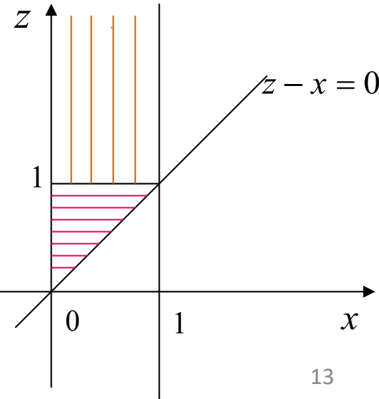
\includegraphics[width=0.5\textwidth]{figures/fig_sum_pdf_plot.png}
    \caption{$Z=X+Y$ 的概率密度函数示意图}
    \label{fig:sum_pdf_plot}
\end{figure}

\subsubsection{商\texorpdfstring{$(Z=Y/X)$}{(Z=Y/X)} 和积\texorpdfstring{$(Z=XY)$}{(Z=XY)} 的分布}

已知 $(X,Y)\sim f(x,y)$，$(x,y)\in\mathbb{R}^{2}$，推导 $Z=Y/X$ 和 $Z=XY$ 的概率密度。

\textbf{(1) $Z=Y/X$ 的概率密度}

\[
F_{Y/X}(z)=P(Y/X\leq z)=\iint_{G_{1}\cup G_{2}}f(x,y)\,dx\,dy,
\]
其中 $G_{1},G_{2}$ 分别为 $x<0$ 和 $x>0$ 时 $y/x\leq z$ 对应的区域。

\begin{figure}[htbp]
    \centering
    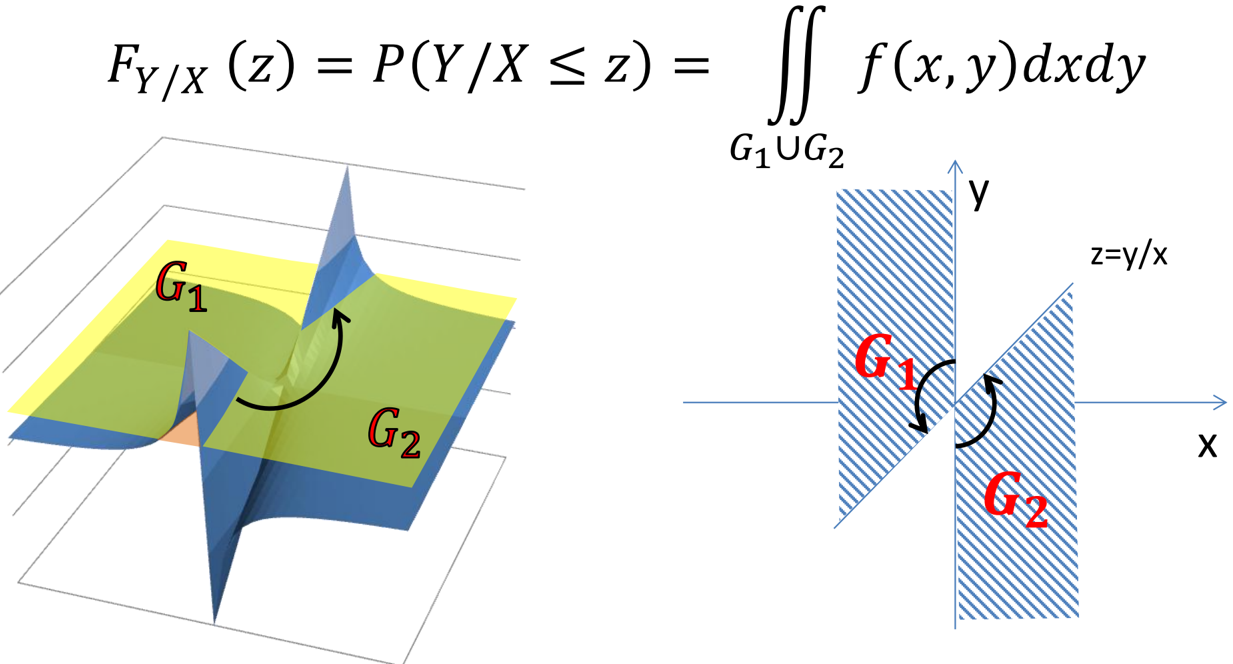
\includegraphics[width=0.6\textwidth]{figures/fig_quotient_regions.png}
    \caption{$Z=Y/X$ 的积分区域 $G_{1}\cup G_{2}$}
    \label{fig:quotient_regions}
\end{figure}

\begin{align*}
F_{Y/X}(z)&=\int_{-\infty}^{0}\int_{zx}^{\infty}f(x,y)\,dy\,dx+\int_{0}^{\infty}\int_{-\infty}^{zx}f(x,y)\,dy\,dx\\
&\quad(\text{令 }y=xu)\\
&=\int_{-\infty}^{0}\int_{z}^{-\infty}xf(x,xu)\,du\,dx+\int_{0}^{\infty}\int_{-\infty}^{z}xf(x,xu)\,du\,dx\\
&=\int_{-\infty}^{0}\int_{-\infty}^{z}-x f(x,xu)\,du\,dx+\int_{0}^{\infty}\int_{-\infty}^{z}x f(x,xu)\,du\,dx\\
&=\int_{-\infty}^{z}\int_{-\infty}^{\infty}|x|f(x,xu)\,dx\,du.
\end{align*}
由概率密度定义得
\[
\boxed{f_{Y/X}(z)=\int_{-\infty}^{\infty}|x|f(x,xz)\,dx}.
\]

\textbf{(2) $Z=XY$ 的概率密度}

当 $z<0$ 时，
\[
F_{XY}(z)=P(XY\leq z)=\iint_{G_{1}\cup G_{2}}f(x,y)\,dx\,dy.
\]

\begin{figure}[htbp]
    \centering
    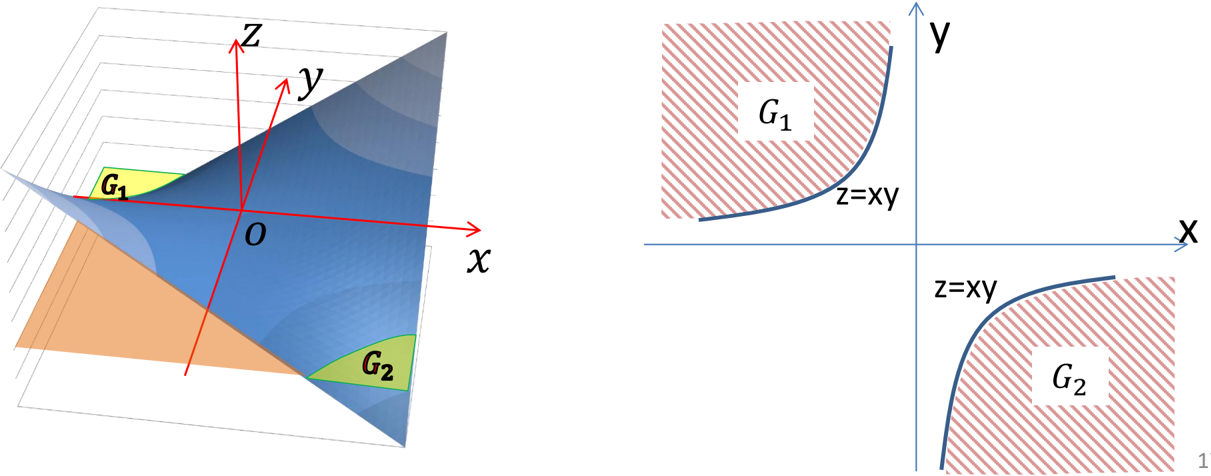
\includegraphics[width=0.6\textwidth]{figures/fig_product_regions.png}
    \caption{$Z=XY$ 的积分区域 $G_{1}\cup G_{2}$（$z<0$）}
    \label{fig:product_regions}
\end{figure}

\begin{align*}
F_{XY}(z)&=\int_{-\infty}^{0^{-}}\int_{z/x}^{\infty}f(x,y)\,dy\,dx+\int_{0^{+}}^{\infty}\int_{-\infty}^{z/x}f(x,y)\,dy\,dx\\
&\quad(\text{令 }y=u/x)\\
&=\int_{-\infty}^{0^{-}}\int_{z}^{-\infty}\frac{1}{x}f\left(x,\frac{u}{x}\right)du\,dx+\int_{0^{+}}^{\infty}\int_{-\infty}^{z}\frac{1}{x}f\left(x,\frac{u}{x}\right)du\,dx\\
&=\int_{-\infty}^{z}\int_{-\infty}^{\infty}\left|\frac{1}{x}\right|f\left(x,\frac{u}{x}\right)dx\,du.
\end{align*}
由概率密度定义得
\[
\boxed{f_{XY}(z)=\int_{-\infty}^{\infty}\left|\frac{1}{x}\right|f\left(x,\frac{z}{x}\right)dx}.
\]

当 $z>0$ 时，可自行类似推导。

\begin{figure}[htbp]
    \centering
    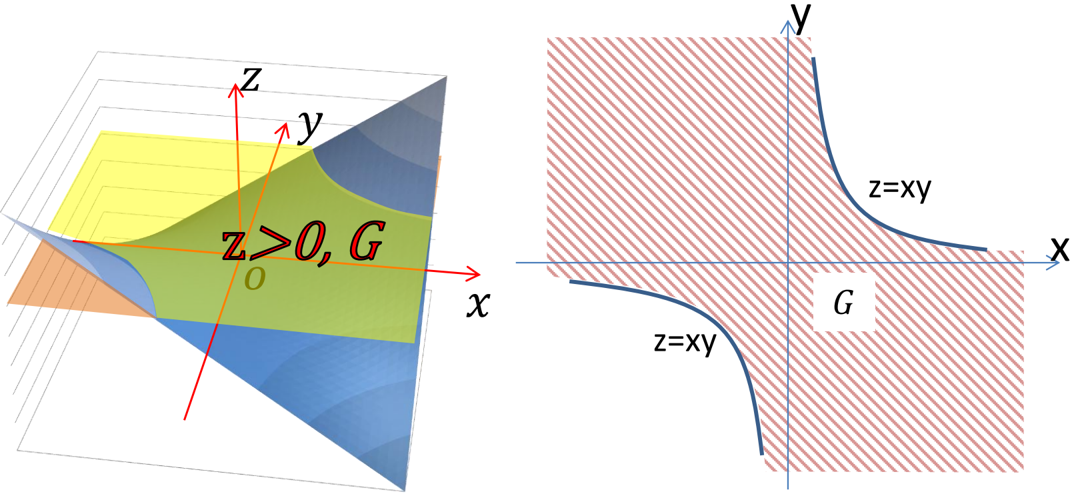
\includegraphics[width=0.6\textwidth]{figures/fig_product_z_positive.png}
    \caption{$Z=XY$ 的积分区域（$z>0$）}
    \label{fig:product_z_positive}
\end{figure}

\subsubsection{相互独立随机变量的极大(小)值的分布}

设 $X,Y$ 是相互独立的随机变量，其分布函数分别为 $F_{X}(x)$ 和 $F_{Y}(y)$，推导 $M=\max\{X,Y\}$ 和 $N=\min\{X,Y\}$ 的分布函数。

由独立性，以及 $M=\max\{X,Y\}$，于是
\[
P\{M\leq z\}=P\{X\leq z,\;Y\leq z\}=P\{X\leq z\}P\{Y\leq z\},
\]
故
\[
\boxed{F_{\max}(z)=F_{X}(z)F_{Y}(z)}.
\]

对于 $N=\min\{X,Y\}$，利用补集关系有
\begin{align*}
P\{N\leq z\}&=1-P\{N>z\}\\
&=1-P\{X>z,\;Y>z\}\\
&=1-P\{X>z\}P\{Y>z\}\\
&=1-[1-F_{X}(z)][1-F_{Y}(z)].
\end{align*}
于是
\[
\boxed{F_{\min}(z)=1-[1-F_{X}(z)][1-F_{Y}(z)]}.
\]

\begin{note}
推广到任意 $n$ 个相互独立的随机变量 $X_{1},X_{2},\dots,X_{n}$，其分布函数分别为 $F_{X_{i}}(x_{i})\;(i=1,2,\dots,n)$，则 $M=\max\{X_{1},X_{2},\dots,X_{n}\}$ 的分布函数为
\[
F_{\max}(z)=\prod_{i=1}^{n}F_{X_{i}}(z).
\]
$N=\min\{X_{1},X_{2},\dots,X_{n}\}$ 的分布函数为
\[
F_{\min}(z)=1-\prod_{i=1}^{n}\bigl[1-F_{X_{i}}(z)\bigr].
\]
这两个分布分别对应不同的可靠性模型。
\end{note}

在实际系统中，经常假定 $X_{1},X_{2},\dots,X_{n}$ 符合独立同分布（iid）$F(x)$，于是有
\[
F_{\max}(z)=[F(z)]^{n},\qquad F_{\min}(z)=1-[1-F(z)]^{n}.
\]
进一步地，若独立同分布的 $X_{i}\;(i=1,2,\dots,n)$ 的密度函数为 $f(x)$，则 $M$ 和 $N$ 对应的密度函数分别为
\[
f_{\max}(z)=n[F(z)]^{n-1}f(z),\qquad f_{\min}(z)=n[1-F(z)]^{n-1}f(z).
\]

\begin{example}[可靠性模型]
设系统 $L$ 由两个相互独立的子系统 $L_{1}$ 和 $L_{2}$ 构成，构成的方式分别为 (1) 串联，(2) 并联，(3) 备份。设 $L_{1},L_{2}$ 的寿命分别为 $X$ 与 $Y$，已知它们的概率密度分别为
\[
f_{X}(x)=
\begin{cases}
\alpha e^{-\alpha x}, & x>0,\\[0.3em]
0, & x\leq 0,
\end{cases}
\qquad
f_{Y}(y)=
\begin{cases}
\beta e^{-\beta y}, & y>0,\\[0.3em]
0, & y\leq 0,
\end{cases}
\]
分别考虑三种情况下系统寿命 $Z$ 的概率密度。
\end{example}

\textbf{分析}：
\begin{itemize}[leftmargin=2em]
    \item \textbf{串联}：一个子系统出故障即导致系统不可用，此时的寿命为 $Z=\min\{X,Y\}$；
    \item \textbf{并联}：可靠性并联模型（热备份），两个子系统均出故障时系统才不可用，此时的寿命为 $Z=\max\{X,Y\}$；
    \item \textbf{备份}：冷备份，两个子系统均出故障时系统才不可用，此时的寿命为 $Z=X+Y$。
\end{itemize}

\begin{figure}[htbp]
    \centering
    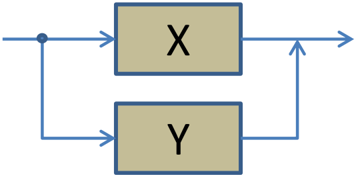
\includegraphics[width=0.3\textwidth]{figures/fig_reliability_series.png}
    \caption{串联系统示意图}
    \label{fig:reliability_series}
\end{figure}

\begin{figure}[htbp]
    \centering
    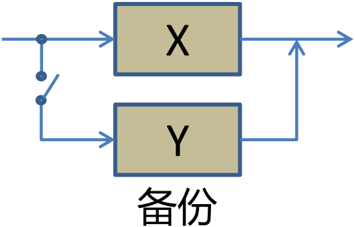
\includegraphics[width=0.3\textwidth]{figures/fig_reliability_parallel.png}
    \caption{并联系统示意图}
    \label{fig:reliability_parallel}
\end{figure}

\begin{figure}[htbp]
    \centering
    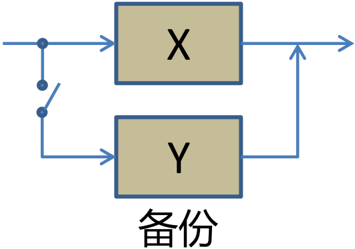
\includegraphics[width=0.3\textwidth]{figures/fig_reliability_backup.png}
    \caption{备份系统示意图}
    \label{fig:reliability_backup}
\end{figure}

\textbf{解}：

(1) \textbf{串联情况}，此时的寿命为 $Z=\min\{X,Y\}$。于是有
\[
F_{\min}(z)=1-[1-F_{X}(z)][1-F_{Y}(z)]
=1-\left[1-\int_{0}^{z}\alpha e^{-\alpha x}\,dx\right]\left[1-\int_{0}^{z}\beta e^{-\beta y}\,dy\right]
=
\begin{cases}
1-e^{-(\alpha+\beta)z}, & z>0,\\[0.3em]
0, & z\leq 0.
\end{cases}
\]
从而概率密度为：
\[
f_{\min}(z)=\frac{dF_{\min}(z)}{dz}=
\begin{cases}
(\alpha+\beta)e^{-(\alpha+\beta)z}, & z>0,\\[0.3em]
0, & z\leq 0.
\end{cases}
\]

(2) \textbf{并联情况}，此时的寿命为 $Z=\max\{X,Y\}$。于是有
\begin{align*}
F_{\max}(z)&=F_{X}(z)F_{Y}(z)\\
&=\int_{0}^{z}\alpha e^{-\alpha x}\,dx\cdot\int_{0}^{z}\beta e^{-\beta y}\,dy\\
&=
\begin{cases}
\bigl(1-e^{-\alpha z}\bigr)\bigl(1-e^{-\beta z}\bigr), & z>0,\\[0.3em]
0, & z\leq 0.
\end{cases}
\end{align*}
从而概率密度为：
\[
f_{\max}(z)=\frac{dF_{\max}(z)}{dz}=
\begin{cases}
\alpha e^{-\alpha z}+\beta e^{-\beta z}-(\alpha+\beta)e^{-(\alpha+\beta)z}, & z>0,\\[0.3em]
0, & z\leq 0.
\end{cases}
\]

(3) \textbf{备份情况}，此时的寿命为 $Z=X+Y$。于是有
\begin{align*}
f_{X+Y}(z)&=\int_{-\infty}^{\infty}f_{X}(z-y)f_{Y}(y)\,dy
=\int_{-\infty}^{\infty}\alpha e^{-\alpha(z-y)}\beta e^{-\beta y}\,dy\\
&=\alpha\beta e^{-\alpha z}\int_{0}^{z}e^{-(\beta-\alpha)y}\,dy
=
\begin{cases}
\dfrac{\alpha\beta}{\beta-\alpha}\bigl(e^{-\alpha z}-e^{-\beta z}\bigr), & z>0,\\[0.8em]
0, & z\leq 0.
\end{cases}
\end{align*}

\section*{本章小结}

\addcontentsline{toc}{section}{本章小结}

\begin{figure}[htbp]
    \centering
    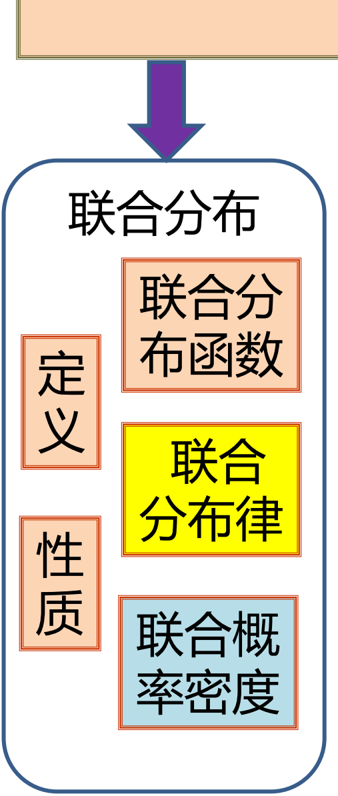
\includegraphics[width=0.3\textwidth]{figures/fig_chapter3_summary.png}
    \caption{第三章知识结构总图}
    \label{fig:chapter3_summary}
\end{figure}

\textbf{要求}：
\begin{itemize}[leftmargin=2em]
    \item 掌握二维随机变量的分布函数的定义及性质；
    \item 掌握二维随机变量的边缘分布与条件分布，及其与联合分布的关系；
    \item 理解随机变量的独立性；
    \item 掌握二维随机变量函数的分布的一般方法以及常用的多维随机变量的和、积、商以及极值等函数的分布。
\end{itemize}

\textbf{核心概念脉络}：

\begin{enumerate}[leftmargin=2em]
    \item \textbf{二维随机变量}：从单个试验同时获得的多个随机变量，$(X,Y)$ 应看作一个整体。联合分布函数 $F(x,y)=P\{X\leq x,\;Y\leq y\}$ 具有单调性、有界性、右连续性和非负性四条基本性质。
    
    \item \textbf{边缘分布}：遍历某一变量所有可能的分布。由联合分布可唯一确定边缘分布，但边缘分布不能唯一确定联合分布。
    
    \item \textbf{条件分布}：联合分布唯一确定边缘分布和条件分布；边缘分布和条件分布各自都不能唯一确定联合分布；一个条件分布和对应的边缘分布一起，能唯一确定联合分布（贝叶斯公式）。
    
    \item \textbf{独立性}：随机变量 $X$ 与 $Y$ 满足 $P\{X\leq x,\;Y\leq y\}=P\{X\leq x\}P\{Y\leq y\}$。独立时联合分布可由边缘分布唯一确定：$F(x,y)=F_{X}(x)F_{Y}(y)$，$f(x,y)=f_{X}(x)f_{Y}(y)$，$p_{ij}=p_{i\cdot}p_{\cdot j}$。
    
    \item \textbf{随机变量的函数的分布}：一般方法为先求分布函数 $F_{Z}(z)=\iint_{g(x,y)\leq z}f(x,y)\,dx\,dy$，再求导得密度。常用结论包括：
    \begin{itemize}
        \item 和分布（卷积公式）：$f_{X+Y}(z)=\int_{-\infty}^{\infty}f(x,z-x)\,dx$；
        \item 商分布：$f_{Y/X}(z)=\int_{-\infty}^{\infty}|x|f(x,xz)\,dx$；
        \item 积分布：$f_{XY}(z)=\int_{-\infty}^{\infty}\frac{1}{|x|}f(x,\frac{z}{x})\,dx$；
        \item 极值分布：$F_{\max}(z)=\prod F_{X_{i}}(z)$，$F_{\min}(z)=1-\prod[1-F_{X_{i}}(z)]$。
    \end{itemize}
\end{enumerate}

\section*{作业}

\addcontentsline{toc}{section}{作业}

教材《概率论与数理统计》第三章（pp.~86--88）：\#18, \#21, \#24, \#29, \#34.

\newpage
\chapter{随机变量的数字特征}

\section{数字特征}

研究概率的目的很大程度在于关心其总体特性。

\begin{example}[投资回报率]
对于投资而言，关心平均回报率。
\end{example}

\begin{example}[学校升学率]
对中学而言，关心学生的升学率；对大学而言，关心毕业生受社会欢迎的程度。
\end{example}

\begin{example}[企业返修率]
对于企业而言，关心产品的返修率。
\end{example}

可以有多种不同的数字特征，本章将关注一些常用的数字特征：
\begin{itemize}[leftmargin=2em]
    \item 数学期望（Expectation）
    \item 方差（Variance）
    \item 协方差（Covariance）
    \item 相关系数（Correlation Coefficient）
    \item 矩（Moment）
\end{itemize}

\section{数学期望}

\subsection{日常生活中的``期望''}

日常生活中的对``期望''的使用：
\begin{enumerate}[label=(\arabic*),leftmargin=2em]
    \item 高考的总分；
    \item 长途旅行时关心目的地平均温度；
    \item 定飞机票时如果连接多个航班，考虑准点率；
    \item 公平问题——赌徒分金问题；
    \item 设计分类器或学习模型时关心错误率/正确率。
\end{enumerate}

\subsubsection*{回顾赌徒分金问题}

梅累和赌友各人下赌注$32$个金币，先赢三局为胜。赌博进行至梅累已赢了两局，而赌友赢了一局时，需要终止赌博，此时的这$64$个金币两人应该怎样分才算合理呢？（假设两人赌技相当）

分析：记梅累赢得次数为$M(n)$，其赌友赢得次数为$F(n)$。

\begin{figure}[htbp]
    \centering
    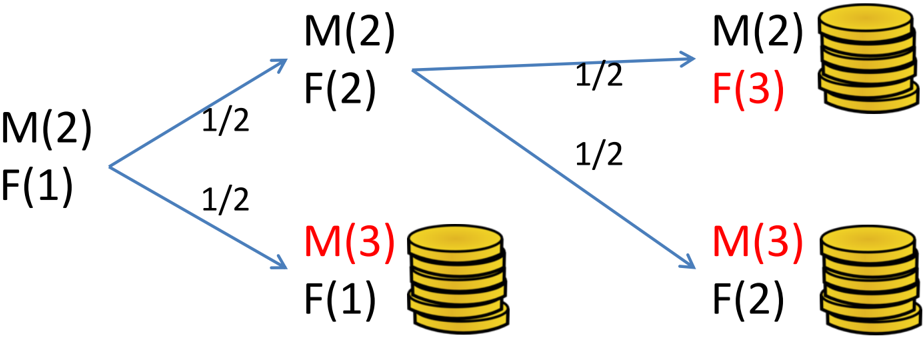
\includegraphics[width=0.5\textwidth]{figures/fig_gambler_tree.png}
    \caption{赌徒分金问题的树状图}
    \label{fig:gambler_tree}
\end{figure}

故在赌技相同的情况下，梅累有$3/4$的希望赢得赌博，梅累的赌友赢得的机会为$1/4$。

因此，梅累能``期望''得到的金币为
\[
64\times\frac{3}{4}+0\times\frac{1}{4}=48.
\]
梅累赌友``期望''得到的金币为
\[
64\times\frac{1}{4}+0\times\frac{3}{4}=16.
\]

从期望的角度，要考虑每种可能的收益/风险。

\subsection{离散型随机变量的数学期望}

\begin{definition}[离散型随机变量的数学期望]
设离散型随机变量$X$的分布律为
\[
P\{X=x_{k}\}=p_{k},\quad k=1,2,\ldots
\]
如果$\sum_{k=1}^{\infty}x_{k}p_{k}$绝对收敛（即$\sum_{k=1}^{\infty}|x_{k}|p_{k}<\infty$），则称级数$\sum_{k=1}^{\infty}x_{k}p_{k}$为随机变量$X$的数学期望（又称均值），记为$E(X)$，即
\[
E(X)=\sum_{k=1}^{\infty}x_{k}p_{k}.
\]
\end{definition}

\begin{note}
$E(X)$是一个实数，而非变量——回到普通大众关心的本质。
\end{note}

\subsubsection*{均值与幸存者偏见}

幸存者偏见意思是指，采样的样本仅来自于幸存者时，存在与实际情况不同的偏差。
\begin{itemize}[leftmargin=2em]
    \item 喝葡萄酒的人长寿；
    \item 二战中的飞机；
    \item 要不要读博士。
\end{itemize}

对策：
\begin{itemize}[leftmargin=2em]
    \item 建立``概率论''思维；
    \item 避免陷入``简单逻辑''。
\end{itemize}

\begin{figure}[htbp]
    \centering
    
\includegraphics[width=0.5\textwidth]{figures/fig_survivor_bias.png}
    \caption{二战中返航飞机弹孔分布示意图（幸存者偏见）}
    \label{fig:survivor_bias}
\end{figure}

\subsubsection*{常见离散型分布的期望}

\textbf{1. 0--1分布}

\begin{table}[htbp]
\centering
\begin{tabular}{@{}ccc@{}}
\toprule
$X$ & $0$ & $1$ \\
\midrule
$p_{X}$ & $1-p$ & $p$ \\
\bottomrule
\end{tabular}
\end{table}

\[
E(X)=1\times p+0\times(1-p)=p.
\]

\textbf{2. 二项分布}

设$X\sim B(n,p)$，即
\[
P(X=k)=\binom{n}{k}p^{k}(1-p)^{n-k},\quad k=0,1,\ldots,n.
\]
则
\[
E(X)=\sum_{k=0}^{n}k\binom{n}{k}p^{k}(1-p)^{n-k}.
\]
注意到$k\binom{n}{k}=n\binom{n-1}{k-1}$，于是
\[
E(X)=np\sum_{k=1}^{n}\binom{n-1}{k-1}p^{k-1}(1-p)^{n-k}=np.
\]

\begin{figure}[htbp]
    \centering
    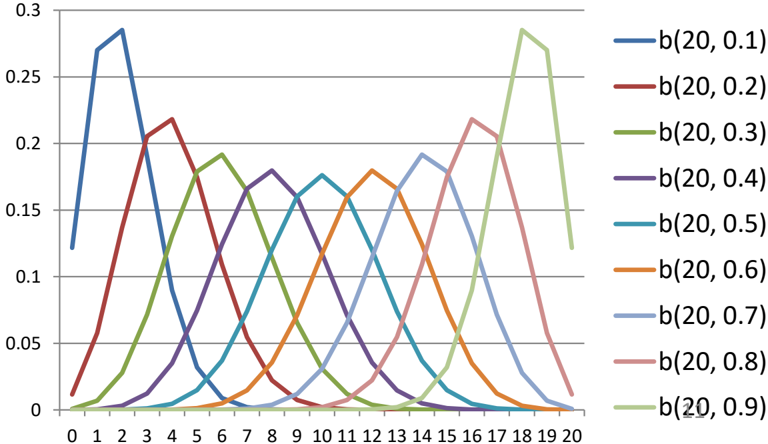
\includegraphics[width=0.5\textwidth]{figures/fig_binomial_pmf.png}
    \caption{二项分布 $b(20,p)$ 的概率质量函数图（$p=0.1,0.2,\ldots,0.9$）}
    \label{fig:binomial_pmf}
\end{figure}

\textbf{3. 几何分布}

设$X\sim g(k,p)$，即
\[
P(X=k)=p(1-p)^{k-1},\quad k=1,2,\ldots
\]
则
\[
E(X)=\sum_{k=1}^{\infty}kp(1-p)^{k-1}=p\sum_{k=1}^{\infty}k(1-p)^{k-1}=\frac{1}{p}.
\]

\begin{figure}[htbp]
    \centering
    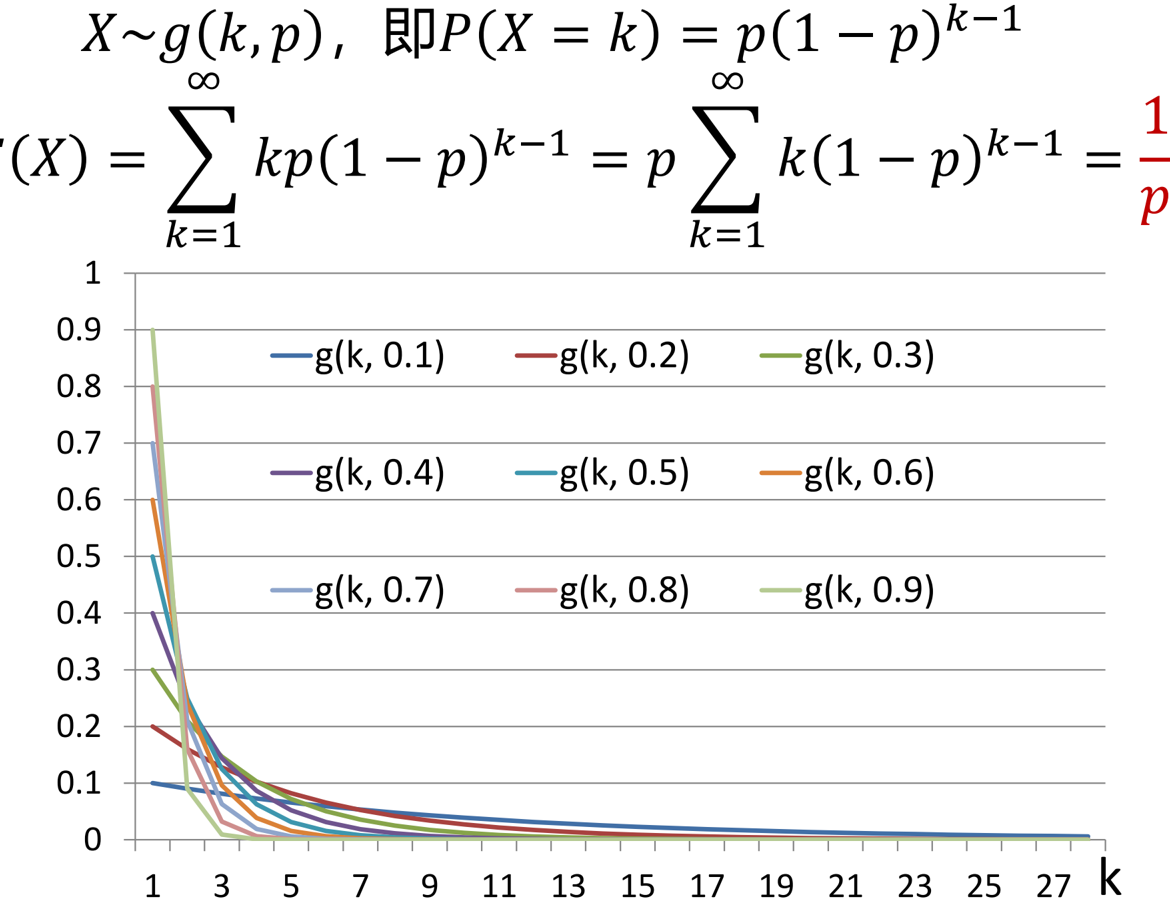
\includegraphics[width=0.5\textwidth]{figures/fig_geometric_pmf.png}
    \caption{几何分布 $g(k,p)$ 的概率质量函数图}
    \label{fig:geometric_pmf}
\end{figure}

\textbf{附：几何分布均值推导}

令$Z_{n}=\sum_{k=1}^{n}kq^{k-1}$（其中$q=1-p$），于是有$Z_{1}=1$，且
\begin{align*}
Z_{n}&=\sum_{k=1}^{n}q^{k-1}+q\sum_{k=2}^{n}(k-1)q^{k-2}\\
&=\sum_{k=1}^{n}q^{k-1}+q\sum_{k=1}^{n-1}kq^{k-1}\\
&=\frac{1-q^{n}}{1-q}+qZ_{n-1}.
\end{align*}
递推可得
\[
\lim_{n\to\infty}Z_{n}=\frac{1}{p^{2}},
\]
故
\[
E(X)=p\cdot\frac{1}{p^{2}}=\frac{1}{p}.
\]

\textbf{4. 泊松分布}

设$X\sim P(\lambda)$，即
\[
P(X=k)=\frac{\lambda^{k}e^{-\lambda}}{k!},\quad k=0,1,2,\ldots
\]
则
\[
E(X)=\sum_{k=1}^{\infty}k\frac{\lambda^{k}e^{-\lambda}}{k!}
=\lambda e^{-\lambda}\sum_{k=1}^{\infty}\frac{\lambda^{k-1}}{(k-1)!}
=\lambda e^{-\lambda}e^{\lambda}=\lambda.
\]

\begin{figure}[htbp]
    \centering
    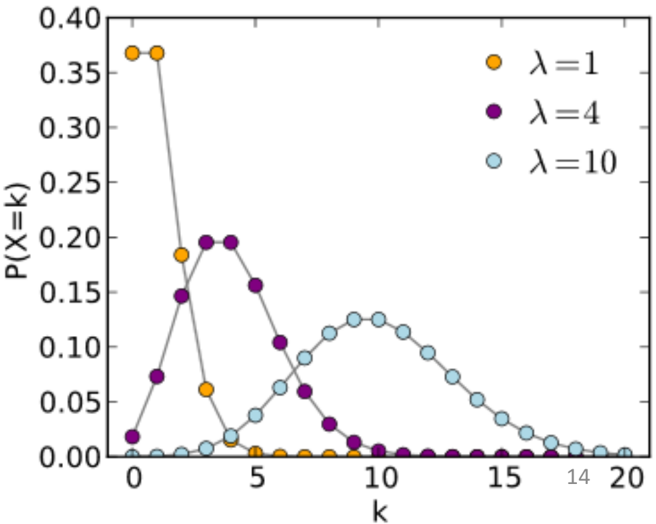
\includegraphics[width=0.5\textwidth]{figures/fig_poisson_pmf.png}
    \caption{泊松分布概率质量函数示意图}
    \label{fig:poisson_pmf}
\end{figure}

\subsubsection*{例子}

\begin{example}[车站候车时间]
按规定，某车站每天$8{:}00$--$9{:}00$，$9{:}00$--$10{:}00$都恰有一辆客车出发，但发车是在三个随机的时刻，且两者发车时间相互独立，其规律为：

\begin{table}[htbp]
\centering
\begin{tabular}{@{}cccc@{}}
\toprule
到站时刻 & $8{:}10$ & $8{:}30$ & $8{:}50$ \\
\midrule
概率 & $1/6$ & $1/2$ & $1/3$ \\
\bottomrule
\end{tabular}
\end{table}

（车2对应$9{:}10,9{:}30,9{:}50$，概率相同）

一旅客$8{:}20$到车站，求他候车时间的数学期望。
\end{example}

\textbf{解}：设旅客的候车时间为$X$（以分计），$X$的分布律为：

\begin{table}[htbp]
\centering
\begin{tabular}{@{}cccccc@{}}
\toprule
$X$ & $10$ ($8{:}30$) & $30$ ($8{:}50$) & $50$ ($9{:}10$) & $70$ ($9{:}30$) & $90$ ($9{:}50$) \\
\midrule
$p_{k}$ & $1/2$ & $1/3$ & $1/6\times 1/6$ & $1/6\times 1/2$ & $1/6\times 1/3$ \\
\bottomrule
\end{tabular}
\end{table}

注意：其中$9{:}00$--$10{:}00$之间车的前提之一是$8{:}00$--$9{:}00$之间的车在$8{:}10$出发。

于是候车的数学期望为
\[
E(X)=10\times\frac{1}{2}+30\times\frac{1}{3}+50\times\frac{1}{36}+70\times\frac{1}{12}+90\times\frac{1}{18}=27.22.
\]

\begin{example}[商店的销售策略]
某商店对某种家用电器的销售采用先使用后付款的方式，记使用寿命为$X$（以年计），规定：
\[
\begin{cases}
X\leq 1, & \text{一台付款}1500\text{元},\\[0.3em]
1<X\leq 2, & \text{一台付款}2000\text{元},\\[0.3em]
2<X\leq 3, & \text{一台付款}2500\text{元},\\[0.3em]
3<X, & \text{一台付款}3000\text{元}.
\end{cases}
\]
设寿命$X$服从指数分布，概率密度为
\[
f(x)=
\begin{cases}
\dfrac{1}{10}e^{-x/10}, & x>0,\\[0.5em]
0, & x\leq 0,
\end{cases}
\]
求该商店一台家电收费$Y$的数学期望。
\end{example}

\textbf{解}：
\begin{align*}
P\{X\leq 1\}&=\int_{0}^{1}\frac{1}{10}e^{-x/10}\,dx=1-e^{-0.1}=0.0952,\\
P\{1<X\leq 2\}&=\int_{1}^{2}\frac{1}{10}e^{-x/10}\,dx=e^{-0.1}-e^{-0.2}=0.0861,\\
P\{2<X\leq 3\}&=\int_{2}^{3}\frac{1}{10}e^{-x/10}\,dx=e^{-0.2}-e^{-0.3}=0.0779,\\
P\{X>3\}&=\int_{3}^{+\infty}\frac{1}{10}e^{-x/10}\,dx=e^{-0.3}=0.7408.
\end{align*}

因而收费的分布律为

\begin{table}[htbp]
\centering
\begin{tabular}{@{}ccccc@{}}
\toprule
$Y$ & $1500$ & $2000$ & $2500$ & $3000$ \\
\midrule
$p_{k}$ & $0.0952$ & $0.0861$ & $0.0779$ & $0.7408$ \\
\bottomrule
\end{tabular}
\end{table}

于是
\[
E(Y)=1500\times 0.0952+2000\times 0.0861+2500\times 0.0779+3000\times 0.7408=2732.15,
\]
即每台的数学期望为$2732.15$元。

\begin{example}[机场爆炸物检查]
机场进行爆炸物检查，可以用两种方法进行：
\begin{enumerate}[label=(\arabic*),leftmargin=2em]
    \item 每个人分别用试纸检测，这就需验$N$次；
    \item $k$个人一组，每组用同一试纸擦拭，然后检查。
    \begin{itemize}
        \item 若呈阴性，直接放行，$k$个人只需验一次；
        \item 若呈阳性，则再对这$k$个人分别进行检查，$k$个人共要$k+1$次。
    \end{itemize}
\end{enumerate}
设每个人接触过爆炸品的概率为$p$，且相互独立。试说明当$p$较小时，选取适当的$k$，按第二种方法可以减少次数，并说明$k$取什么值时最适宜。
\end{example}

\begin{figure}[htbp]
    \centering
    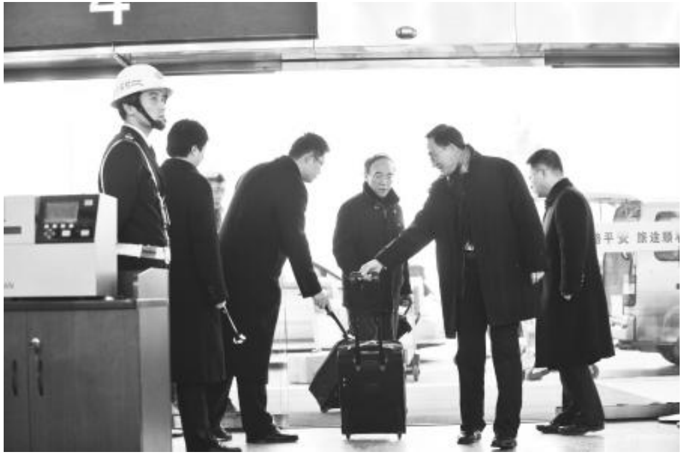
\includegraphics[width=0.5\textwidth]{figures/fig_airport_security.png}
    \caption{机场安检示意图}
    \label{fig:airport_security}
\end{figure}

\textbf{解}：每个人未接触过爆炸品的概率为$q=1-p$。

设以$k$个人为一组时，组内每人化验的次数为$X$，则：

\begin{table}[htbp]
\centering
\begin{tabular}{@{}ccc@{}}
\toprule
$X$ & $1/k$ & $(k+1)/k$ \\
\midrule
$p_{k}$ & $q^{k}$ & $1-q^{k}$ \\
\bottomrule
\end{tabular}
\end{table}

于是
\[
E(X)=\frac{1}{k}q^{k}+\frac{k+1}{k}(1-q^{k})=1+\frac{1}{k}-q^{k}.
\]

于是只要$\frac{1}{k}-q^{k}<0$，即可减少平均次数。

最佳分组大小与$q$的关系如下图所示。

\begin{figure}[htbp]
    \centering
    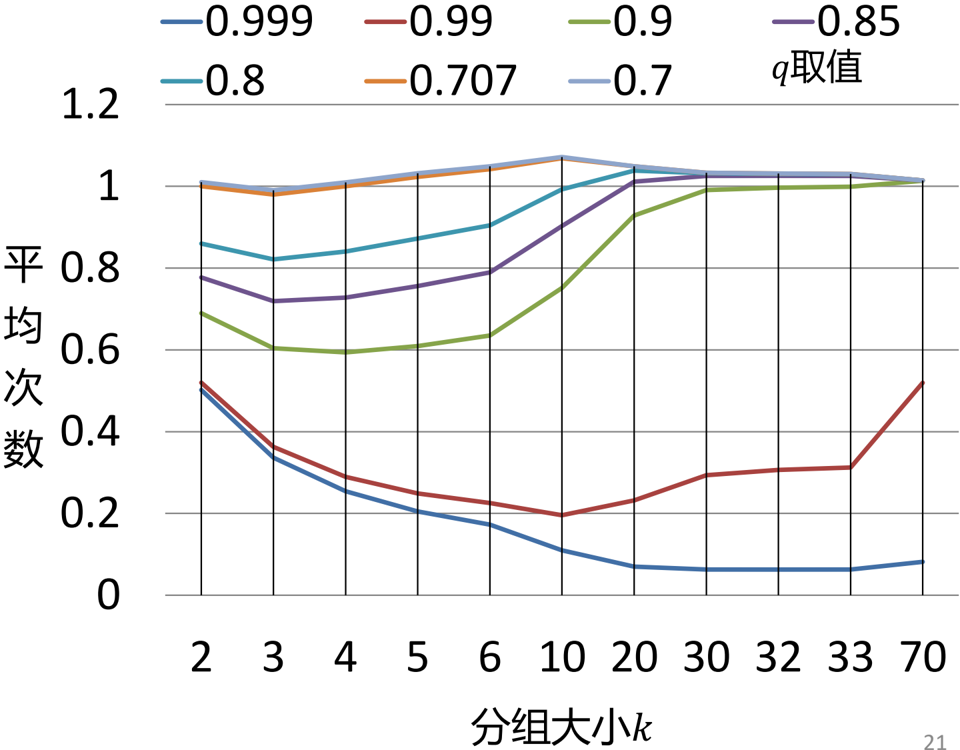
\includegraphics[width=0.5\textwidth]{figures/fig_optimal_group_size.png}
    \caption{最佳分组大小与 $q$ 的关系图（平均次数随分组大小 $k$ 变化的曲线，$q$ 取不同值）}
    \label{fig:optimal_group_size}
\end{figure}

可见当$p$较小（例如，$\leq 0.01$）时，$10\sim 20$人的分组是非常有效的。

\subsection{连续型随机变量的数学期望}

\begin{definition}[连续型随机变量的数学期望]
设连续型随机变量$X$的概率密度函数为$f(x)$，如果
\[
\int_{-\infty}^{+\infty}|x|f(x)\,dx
\]
绝对收敛，则称
\[
\int_{-\infty}^{+\infty}xf(x)\,dx
\]
的值为随机变量$X$的数学期望，记为
\[
E(X)=\int_{-\infty}^{+\infty}xf(x)\,dx.
\]
\end{definition}

\begin{example}[服务等待时间]
设顾客在某银行的窗口等待服务的时间$X$（以分计）服从指数分布，其概率密度为
\[
f(x)=
\begin{cases}
\dfrac{e^{-x/5}}{5}, & x>0,\\[0.5em]
0, & x\leq 0.
\end{cases}
\]
试求顾客等待服务的平均时间。
\end{example}

\textbf{解}：
\[
E(X)=\int_{-\infty}^{+\infty}xf(x)\,dx=\int_{0}^{+\infty}\frac{x e^{-x/5}}{5}\,dx
=5\left(-\frac{x}{5}-1\right)e^{-x/5}\Big|_{0}^{\infty}=5.
\]

\subsubsection*{常见连续型分布的期望}

\textbf{1. 均匀分布}

设$X\sim U(a,b)$，即
\[
f(x)=
\begin{cases}
\dfrac{1}{b-a}, & a<x<b,\\[0.5em]
0, & \text{其他}.
\end{cases}
\]
则
\[
E(X)=\int_{-\infty}^{+\infty}xf(x)\,dx=\int_{a}^{b}\frac{x}{b-a}\,dx=\frac{b^{2}-a^{2}}{2(b-a)}=\frac{a+b}{2}.
\]

\textbf{2. 指数分布}

设$X\sim\text{Exponential}(\lambda)$，即
\[
f(x)=
\begin{cases}
\lambda e^{-\lambda x}, & x>0,\\[0.3em]
0, & x\leq 0.
\end{cases}
\]
则
\[
E(X)=\int_{0}^{+\infty}x\lambda e^{-\lambda x}\,dx
=\lambda\left(-\frac{x}{\lambda}-\frac{1}{\lambda^{2}}\right)e^{-\lambda x}\Big|_{0}^{+\infty}
=\frac{1}{\lambda}.
\]

\begin{figure}[htbp]
    \centering
    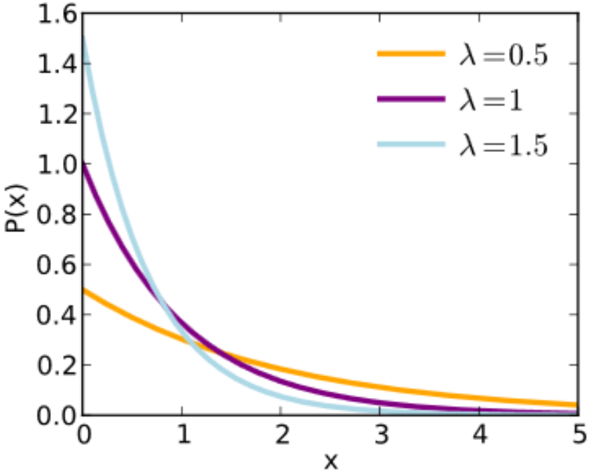
\includegraphics[width=0.5\textwidth]{figures/fig_exponential_pdf_params.png}
    \caption{指数分布概率密度函数图（$\lambda=0.5,1,1.5$）}
    \label{fig:exponential_pdf_params}
\end{figure}

\textbf{3. 正态分布}

设$X\sim N(\mu,\sigma^{2})$，即
\[
f(x)=\frac{1}{\sqrt{2\pi}\sigma}e^{-\frac{(x-\mu)^{2}}{2\sigma^{2}}}.
\]
则
\begin{align*}
E(X)&=\int_{-\infty}^{+\infty}x\frac{1}{\sqrt{2\pi}\sigma}e^{-\frac{(x-\mu)^{2}}{2\sigma^{2}}}\,dx\\
&=\int_{-\infty}^{+\infty}\frac{x-\mu}{\sqrt{2\pi}\sigma}e^{-\frac{(x-\mu)^{2}}{2\sigma^{2}}}\,dx
+\int_{-\infty}^{+\infty}\frac{\mu}{\sqrt{2\pi}\sigma}e^{-\frac{(x-\mu)^{2}}{2\sigma^{2}}}\,dx\\
&=\frac{\mu}{\sqrt{2\pi}\sigma}\int_{-\infty}^{+\infty}e^{-\frac{u^{2}}{2\sigma^{2}}}\,du\quad(u=x-\mu)\\
&=\mu.
\end{align*}
（其中利用了极坐标代换计算$[E(X)]^{2}=\mu^{2}$以验证归一性）

\subsection{随机变量函数的数学期望}

\begin{theorem}[一维随机变量函数的期望]
设$Y$是随机变量$X$的函数，即$Y=g(X)$，$g(x)$是连续函数。
\begin{enumerate}[label=(\arabic*),leftmargin=2em]
    \item 若$X$是离散型随机变量，且其概率分布为$P\{X=x_{i}\}=p_{i}$，$i=1,2,\ldots$。若$\sum_{i=1}^{\infty}g(x_{i})p_{i}$绝对收敛，则$Y$的数学期望为
    \[
    E(Y)=E[g(X)]=\sum_{i=1}^{\infty}g(x_{i})p_{i}.
    \]
    \item 若$X$是连续型随机变量，且其概率密度为$f(x)$。若$\int_{-\infty}^{+\infty}g(x)f(x)\,dx$绝对收敛，则$Y$的数学期望为
    \[
    E(Y)=E[g(X)]=\int_{-\infty}^{+\infty}g(x)f(x)\,dx.
    \]
\end{enumerate}
\end{theorem}

\begin{note}
这一定理的价值在于给出了求$E(Y)$时，不必算出$Y$的分布律或概率密度，而是直接利用$X$的分布律或概率密度即可。
\end{note}

从一维到二维随机变量的扩展，有下面的定理：

\begin{theorem}[二维随机变量函数的期望]
设$Z$是随机变量$X,Y$的函数，即$Z=g(X,Y)$，$g(x,y)$是连续函数。
\begin{enumerate}[label=(\arabic*),leftmargin=2em]
    \item 若二维离散型随机变量$(X,Y)$的分布律为
    \[
    P(X=x_{i},Y=y_{j})=p_{ij},\quad i,j=1,2,\ldots
    \]
    若$\sum_{i=1}^{\infty}\sum_{j=1}^{\infty}g(x_{i},y_{j})p_{ij}$绝对收敛，则$Z$的数学期望为
    \[
    E(Z)=E[g(X,Y)]=\sum_{i=1}^{\infty}\sum_{j=1}^{\infty}g(x_{i},y_{j})p_{ij}.
    \]
    \item 若二维连续型随机变量$(X,Y)$的概率密度为$f(x,y)$，若
    \[
    \int_{-\infty}^{+\infty}\int_{-\infty}^{+\infty}g(x,y)f(x,y)\,dx\,dy
    \]
    绝对收敛，则$Z$的数学期望为
    \[
    E(Z)=E[g(X,Y)]=\int_{-\infty}^{+\infty}\int_{-\infty}^{+\infty}g(x,y)f(x,y)\,dx\,dy.
    \]
\end{enumerate}
\end{theorem}

\begin{example}[飞机机翼的正压力]
设风速$V$在$(0,a)$上服从均匀分布，即具有概率密度
\[
f(v)=
\begin{cases}
\dfrac{1}{a}, & 0<v<a,\\[0.5em]
0, & \text{其他}.
\end{cases}
\]
又设飞机机翼受到的正压力$W$是$V$的函数，$W=kV^{2}$，$k>0$是常数，求$W$的数学期望。
\end{example}

\textbf{解}：由上述定理有
\[
E(W)=\int_{0}^{a}kv^{2}f(v)\,dv=\int_{0}^{a}\frac{kv^{2}}{a}\,dv=\frac{1}{3}ka^{2}.
\]

\begin{example}[二维随机变量函数的期望]
设随机变量$(X,Y)$的概率密度为
\[
f(x,y)=
\begin{cases}
\dfrac{3}{2x^{3}y^{2}}, & \dfrac{1}{x}<y<x,\;x>1,\\[0.5em]
0, & \text{其他}.
\end{cases}
\]
求数学期望$E(Y)$，$E\!\left(\dfrac{1}{XY}\right)$。
\end{example}

\begin{figure}[htbp]
    \centering
    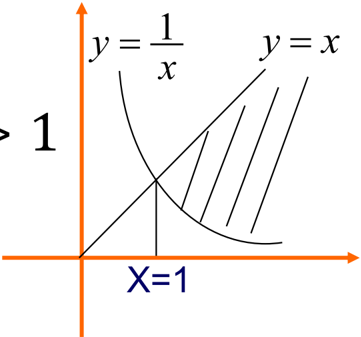
\includegraphics[width=0.5\textwidth]{figures/fig_integration_region.png}
    \caption{积分区域示意图（$y=1/x, y=x, x=1$ 围成的区域）}
    \label{fig:integration_region}
\end{figure}

\textbf{解}：
\[
E(Y)=\int_{-\infty}^{+\infty}\int_{-\infty}^{+\infty}yf(x,y)\,dy\,dx
=\int_{1}^{+\infty}\int_{1/x}^{x}\frac{3}{2x^{3}y}\,dy\,dx
=3\int_{1}^{+\infty}\frac{\ln x}{x^{3}}\,dx=\frac{3}{4}.
\]

另外，
\[
E\!\left(\frac{1}{XY}\right)=\int_{1}^{+\infty}\int_{1/x}^{x}\frac{3}{2x^{4}y^{3}}\,dy\,dx
=\frac{3}{4}\int_{1}^{+\infty}\left(\frac{1}{x^{2}}-\frac{1}{x^{6}}\right)dx=\frac{3}{5}.
\]

\begin{note}
另外的解法，按照定义，先求出$f_{Y}(y)$，之后再求出$E(Y)=\int_{-\infty}^{+\infty}yf_{Y}(y)\,dy$。
\end{note}

\begin{example}[生产决策]
某航空公司打算开辟新航线，并考虑航班的运力，估计每售出一张机票可获利$300$元，而出现一个空座将导致$700$元的损失，预计每周旅行的乘客数$Y$服从指数分布
\[
f_{Y}(y)=
\begin{cases}
\lambda e^{-\lambda y}, & y>0,\\[0.3em]
0, & y\leq 0.
\end{cases}
\]
试为这条航线确定每周需要的座位数。
\end{example}

\begin{figure}[htbp]
    \centering
    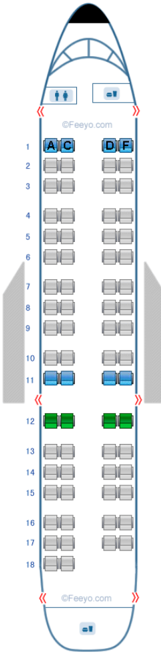
\includegraphics[width=0.25\textwidth]{figures/fig_production_decision.png}
    \caption{生产决策示意图}
    \label{fig:production_decision}
\end{figure}

\textbf{解}：设安排的座位数为$x$，则获利（损失）函数如下
\[
g(y)=
\begin{cases}
300y-700(x-y), & y<x,\\[0.3em]
300x, & y\geq x.
\end{cases}
\]

预期获益（损失）$E[g(y)]$为
\[
E[g(y)]=\int_{0}^{x}[300y-700(x-y)]\lambda e^{-\lambda y}\,dy+\int_{x}^{\infty}300x\lambda e^{-\lambda y}\,dy.
\]
计算得
\[
E[g(y)]=\frac{1000}{\lambda}(1-e^{-\lambda x})-700x.
\]

令
\[
\frac{dE(g(y))}{dx}=1000e^{-\lambda x}-700=0,
\]
得
\[
x=-\frac{1}{\lambda}\ln 0.7\approx\frac{0.3567}{\lambda}.
\]

由于
\[
\frac{d^{2}E(g(y))}{dx^{2}}=-1000\lambda e^{-\lambda x}<0,
\]
故此时有最大收益（最小损失）。

于是收益（损失）为
\[
\frac{1000}{\lambda}(1-e^{-0.3567})-700x=\frac{300.0173711}{\lambda}-700x.
\]

如果$\lambda=0.0001$，则每周安排大约$3567$个座位，预计可以取得最佳效益，大约获利$503{,}273.71$元。

\subsubsection*{数学期望的特性}

\begin{property}[数学期望的基本性质]
\begin{enumerate}[label=\arabic*.,leftmargin=2em]
    \item 设$C$是常数，则有$E(C)=C$。
    
    \item 设$X$是一个随机变量，$C$是常数，则有
    \[
    E(CX)=CE(X).
    \]
    
    \item 设$X,Y$是两个随机变量，则有
    \[
    E(X+Y)=E(X)+E(Y).
    \]
    
    \item 设$X,Y$是相互独立的随机变量，则有
    \[
    E(XY)=E(X)E(Y).
    \]
\end{enumerate}
\end{property}

\textbf{证明}（性质3）：
\[
E(X+Y)=\int_{-\infty}^{+\infty}\int_{-\infty}^{+\infty}(x+y)f(x,y)\,dx\,dy
=\int_{-\infty}^{+\infty}\int_{-\infty}^{+\infty}xf(x,y)\,dx\,dy
+\int_{-\infty}^{+\infty}\int_{-\infty}^{+\infty}yf(x,y)\,dx\,dy
=E(X)+E(Y).
\]

\textbf{证明}（性质4）：
\[
E(XY)=\int_{-\infty}^{+\infty}\int_{-\infty}^{+\infty}xyf(x,y)\,dx\,dy
=\int_{-\infty}^{+\infty}\int_{-\infty}^{+\infty}xyf_{X}(x)f_{Y}(y)\,dx\,dy
=E(X)E(Y).
\]

将上述性质结合有：
\[
E(aX+bY+c)=aE(X)+bE(Y)+c.
\]
这一性质可推广至任意有限个随机变量线性组合的情况。

\begin{example}[电梯停留层数]
酒店客房均匀分布在$2$--$11$层，电梯从一层出发载有$20$位客人，假定没有来自电梯外部的停留请求，以$X$表示停的次数，求$X$的数学期望（设各位客人在各层离开电梯是等可能的，并设各客人是相互独立的）。
\end{example}

\textbf{解}：引入随机变量
\[
X_{i}=
\begin{cases}
0, & \text{第}i+1\text{层无人离开},\\[0.3em]
1, & \text{第}i+1\text{层有人离开},
\end{cases}
\quad i=1,2,\ldots,10.
\]

于是
\[
X=X_{1}+X_{2}+\cdots+X_{10}.
\]
\[
E(X_{i})=P(X_{i}=1)=1-\left(\frac{9}{10}\right)^{20}.
\]
故
\[
E(X)=\sum_{i=1}^{10}E(X_{i})=10\left[1-\left(\frac{9}{10}\right)^{20}\right]\approx 8.784.
\]

\begin{note}
将$X$分解成数个随机变量之和，然后利用随机变量和的数学期望等于随机变量数学期望之和来求数学期望。
\end{note}

\subsubsection*{关于期望的直觉理解}

\begin{itemize}[leftmargin=2em]
    \item 期望就是加权平均；
    \item 加权的对象就是随机变量或随机变量的函数；
    \item ``权''就是概率的分布律，或概率密度函数。
\end{itemize}

\subsubsection*{期望的统一表达}

\begin{definition}[期望的统一表达]
$X$的期望值定义为
\[
E(X)=\int x\,dF(x)=
\begin{cases}
\sum_{k=1}^{\infty}x_{k}p_{k}, & \text{离散型},\\[0.5em]
\int_{-\infty}^{+\infty}xf(x)\,dx, & \text{连续型}.
\end{cases}
\]
如果上式绝对收敛，则称其值为随机变量$X$的数学期望。
\end{definition}

\section{方差}

\begin{example}[投资与风险]
对于投资而言，关心平均回报率，但也关心可能的风险。
\end{example}

\begin{example}[学校教育的质量]
对中学而言，关心学生的升学率，但也关心最好考取好学校的人数，和落在最差的那一部分人数；对大学而言关心毕业生受社会欢迎的程度，但也关心产生的各类领袖人数等。
\end{example}

\begin{example}[企业产品质量]
对于企业而言，关心产品的返修率，但也关心极端故障（需要危机公关），和极端的优秀产品（用来做广告）。
\end{example}

考虑一个问题：如果你是射击队教练，有两个队员，一个肯定能进前$8$名，另一位发挥好能拿冠军，发挥失常则无缘决赛，现在只有一个参赛名额，你会选择哪一位？

\begin{example}[灯泡质量]
设有一批灯泡寿命为：一半约$950$小时，另一半约$1050$小时，平均寿命为$1000$小时；另一批灯泡寿命为：一半约$1300$小时，另一半约$700$小时，平均寿命为$1000$小时。哪批灯泡的质量更好？
\end{example}

单从平均寿命这一指标无法判断，进一步考察灯泡寿命$X$与均值$1000$小时的偏离程度。

方差——正是体现这种意义的数学特征。

\begin{definition}[方差]
设$X$是一个随机变量，若$E\{[X-E(X)]^{2}\}$存在，则称其为$X$的\textbf{方差}，记为$D(X)$或$\mathrm{Var}(X)$，即
\[
D(X)=\mathrm{Var}(X)=E\{[X-E(X)]^{2}\}.
\]
将$\sqrt{D(X)}$记为$\sigma(X)$，称为$X$的\textbf{标准差}或\textbf{均方差}，它是与随机变量$X$具有相同量纲的量。
\end{definition}

方差$D(X)$刻画了$X$取值的分散程度，它是衡量$X$取值分散程度的度量。若$X$取值集中，则$D(X)$较小；反之，若$X$取值比较分散，则$D(X)$较大。

\subsubsection*{方差的几何解释}

考虑分布$(2,4,4,4,5,5,7,9)$：
\begin{enumerate}[label=\arabic*.,leftmargin=2em]
    \item 分布的几何图示；
    \item 分布的均值；
    \item 每个点到均值的距离为边的正方形；
    \item 将所有正方形重排成一边长为$n$（样本点数）的矩形，另一边长为方差$\sigma^{2}$。
\end{enumerate}

\begin{figure}[htbp]
    \centering
    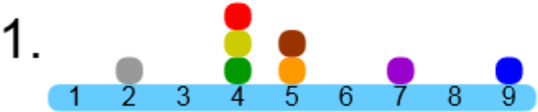
\includegraphics[width=0.5\textwidth]{figures/fig_variance_geometry.png}
    \caption{方差的几何解释示意图}
    \label{fig:variance_geometry}
\end{figure}

对离散型随机变量$X$，其分布律为$P(X=x_{k})=p_{k}$，对应的方差为
\[
D(X)=\sum_{k=1}^{\infty}[x_{k}-E(X)]^{2}p_{k}.
\]
对连续型随机变量$X$，其概率密度为$f(x)$，对应的方差为
\[
D(X)=\int_{-\infty}^{+\infty}[x-E(X)]^{2}f(x)\,dx.
\]
统一表达：
\[
D(X)=\int[x-E(X)]^{2}\,dF(x).
\]

注意下面的方法推导过程，由此产生另一个计算的方法：
\begin{align*}
D(X)&=E\{[X-E(X)]^{2}\}\\
&=E\{X^{2}-2XE(X)+[E(X)]^{2}\}\\
&=E(X^{2})-2E(X)E(X)+[E(X)]^{2}\\
&=E(X^{2})-[E(X)]^{2}.
\end{align*}

\begin{example}[随机变量的标准化]
设随机变量$X$具有数学期望$E(X)=\mu$，方差$D(X)=\sigma^{2}\neq 0$，记
\[
X^{*}=\frac{X-\mu}{\sigma},
\]
并称为$X$的\textbf{标准化变量}，证明$E(X^{*})=0$，$D(X^{*})=1$。
\end{example}

\textbf{证明}：
\[
E(X^{*})=\frac{1}{\sigma}E(X-\mu)=\frac{1}{\sigma}[E(X)-\mu]=0.
\]
\[
D(X^{*})=E[(X^{*})^{2}]-[E(X^{*})]^{2}
=E\left[\left(\frac{X-\mu}{\sigma}\right)^{2}\right]
=\frac{1}{\sigma^{2}}E[(X-\mu)^{2}]
=\frac{\sigma^{2}}{\sigma^{2}}=1.
\]

\subsubsection*{常见分布的方差}

\textbf{1. 0--1分布}

已知$E(X)=p$，且
\[
E(X^{2})=0^{2}\cdot(1-p)+1^{2}\cdot p=p.
\]
故
\[
D(X)=E(X^{2})-[E(X)]^{2}=p-p^{2}=p(1-p).
\]

\textbf{2. 二项分布}

设$X\sim B(n,p)$，已知$E(X)=np$。
\[
E(X^{2})=\sum_{k=0}^{n}k^{2}\binom{n}{k}p^{k}(1-p)^{n-k}.
\]
利用$k\binom{n}{k}=n\binom{n-1}{k-1}$，有
\begin{align*}
E(X^{2})&=\sum_{k=1}^{n}nk\binom{n-1}{k-1}p^{k}(1-p)^{n-k}\\
&=np\sum_{k=1}^{n}(k-1)\binom{n-1}{k-1}p^{k-1}(1-p)^{n-k}+np\\
&=n(n-1)p^{2}\sum_{k=2}^{n}\binom{n-2}{k-2}p^{k-2}(1-p)^{n-k}+np\\
&=n(n-1)p^{2}+np.
\end{align*}
故
\[
D(X)=E(X^{2})-[E(X)]^{2}=n(n-1)p^{2}+np-(np)^{2}=np(1-p).
\]

\begin{figure}[htbp]
    \centering
    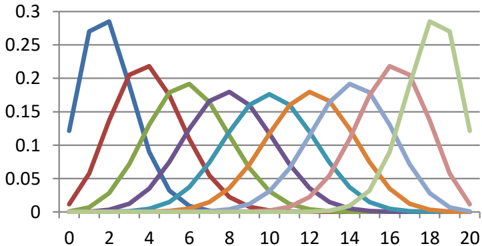
\includegraphics[width=0.5\textwidth]{figures/fig_binomial_variance.png}
    \caption{二项分布方差示意图}
    \label{fig:binomial_variance}
\end{figure}

\textbf{3. 泊松分布}

设$X\sim P(\lambda)$，已知$E(X)=\lambda$。
\[
E(X^{2})=\sum_{k=1}^{\infty}k^{2}\frac{\lambda^{k}e^{-\lambda}}{k!}
=\sum_{k=1}^{\infty}k(k-1)\frac{\lambda^{k}e^{-\lambda}}{k!}
+\sum_{k=1}^{\infty}k\frac{\lambda^{k}e^{-\lambda}}{k!}
=\lambda^{2}+\lambda.
\]
故
\[
D(X)=E(X^{2})-[E(X)]^{2}=\lambda^{2}+\lambda-\lambda^{2}=\lambda.
\]

\begin{note}
泊松分布的期望和方差均是$\lambda$。
\end{note}

\begin{figure}[htbp]
    \centering
    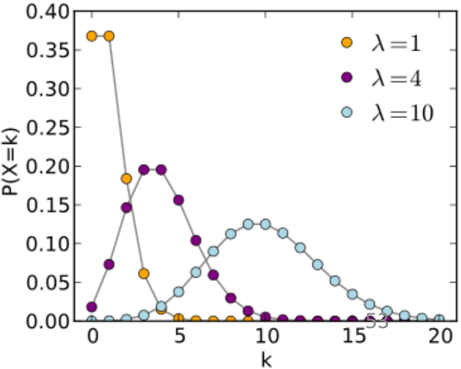
\includegraphics[width=0.5\textwidth]{figures/fig_poisson_pmf_variance.png}
    \caption{泊松分布概率质量函数示意图}
    \label{fig:poisson_pmf_variance}
\end{figure}

\textbf{4. 均匀分布}

设$X\sim U(a,b)$，已知$E(X)=\dfrac{a+b}{2}$。
\[
E(X^{2})=\int_{a}^{b}\frac{x^{2}}{b-a}\,dx=\frac{b^{3}-a^{3}}{3(b-a)}=\frac{a^{2}+b^{2}+ab}{3}.
\]
故
\[
D(X)=E(X^{2})-[E(X)]^{2}
=\frac{a^{2}+b^{2}+ab}{3}-\frac{(a+b)^{2}}{4}
=\frac{(b-a)^{2}}{12}.
\]

\textbf{5. 指数分布}

设$X\sim\text{Exponential}(\lambda)$，已知$E(X)=\dfrac{1}{\lambda}$。
\[
E(X^{2})=\int_{0}^{+\infty}x^{2}\lambda e^{-\lambda x}\,dx
=\lambda e^{-\lambda x}\left(-\frac{x^{2}}{\lambda}-\frac{2x}{\lambda^{2}}-\frac{2}{\lambda^{3}}\right)\Big|_{0}^{+\infty}
=\frac{2}{\lambda^{2}}.
\]
故
\[
D(X)=E(X^{2})-[E(X)]^{2}=\frac{2}{\lambda^{2}}-\frac{1}{\lambda^{2}}=\frac{1}{\lambda^{2}}.
\]

\begin{figure}[htbp]
    \centering
    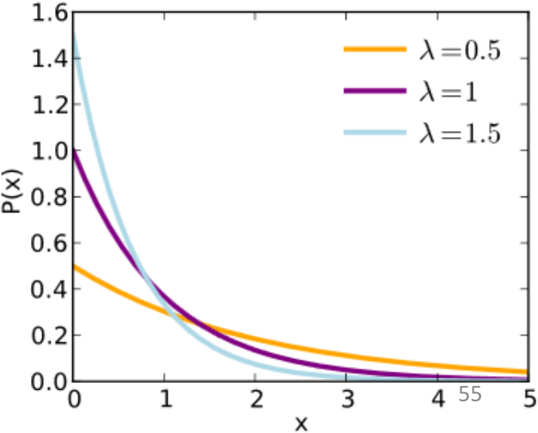
\includegraphics[width=0.5\textwidth]{figures/fig_exponential_pdf_variance.png}
    \caption{指数分布概率密度函数图}
    \label{fig:exponential_pdf_variance}
\end{figure}

\section*{作业}

\addcontentsline{toc}{section}{作业}

教材《概率论与数理统计》第四章（pp.~114--115）：\#9，\#14，\#18。

教材《概率论及其应用》（pp.~182--183/197--201）：\#8，\#19，\#38。

\subsection{方差的性质}

\begin{property}[方差的基本性质]
\begin{enumerate}[label=\arabic*.,leftmargin=2em]
    \item 设$C$是常数，则有$D(C)=0$。
    
    \textbf{证明}：
    \[
    D(C)=E\{[C-E(C)]^{2}\}=0.
    \]
    
    \item 设$X$是一个随机变量，$C$是常数，则有
    \[
    D(CX)=C^{2}D(X).
    \]
    
    \textbf{证明}：
    \[
    D(CX)=E[(CX)^{2}]-[E(CX)]^{2}=C^{2}E(X^{2})-C^{2}[E(X)]^{2}=C^{2}D(X).
    \]
    
    \item 设$X,Y$是两个随机变量，则有
    \[
    D(X+Y)=D(X)+D(Y)+2E\{[X-E(X)][Y-E(Y)]\}.
    \]
    特别地，若$X,Y$相互独立，则有
    \[
    D(X+Y)=D(X)+D(Y).
    \]
    
    \textbf{证明}：
    \begin{align*}
    D(X+Y)&=E\{[(X+Y)-E(X+Y)]^{2}\}\\
    &=E\{[(X-E(X))+(Y-E(Y))]^{2}\}\\
    &=E\{[X-E(X)]^{2}\}+E\{[Y-E(Y)]^{2}\}\\
    &\quad+2E\{[X-E(X)][Y-E(Y)]\}\\
    &=D(X)+D(Y)+2\mathrm{Cov}(X,Y).
    \end{align*}
    若$X,Y$相互独立，$X-E(X)$与$Y-E(Y)$相互独立，有
    \[
    E\{[X-E(X)][Y-E(Y)]\}=E[X-E(X)]\cdot E[Y-E(Y)]=0,
    \]
    于是$D(X+Y)=D(X)+D(Y)$。
    
    \item 将上述性质结合，若$X,Y$相互独立，$a,b,c$是常数，则有
    \[
    D(aX+bY+c)=a^{2}D(X)+b^{2}D(Y).
    \]
    这一性质可推广至任意有限个相互独立的随机变量线性组合的情况。
    
    \item $D(X)=0\Leftrightarrow P\{X=E(X)\}=1$。
\end{enumerate}
\end{property}

\begin{example}[活塞与气缸]
设活塞直径（cm）$X\sim N(22.40,0.03^{2})$，气缸直径$Y\sim N(22.50,0.04^{2})$，$X,Y$相互独立，求任取一只活塞和一只气缸，活塞能装入气缸的概率。
\end{example}

\textbf{解}：由正态分布和的分布规律，有
\[
X-Y\sim N(-0.10,0.05^{2}).
\]
于是
\begin{align*}
P\{X\leq Y\}&=P\{X-Y\leq 0\}\\
&=P\left\{\frac{(X-Y)-(-0.10)}{0.05}\leq\frac{0-(-0.10)}{0.05}\right\}\\
&=\Phi(2)=0.9772.
\end{align*}

\begin{theorem}[样本均值与样本方差]
令$X_{1},X_{2},\ldots,X_{n}$为iid随机变量，$\mu=E(X_{i})$，$\sigma^{2}=D(X_{i})$。定义样本均值为
\[
\bar{X}_{n}=\frac{1}{n}\sum_{i=1}^{n}X_{i},
\]
样本方差为
\[
S_{n}^{2}=\frac{1}{n-1}\sum_{i=1}^{n}(X_{i}-\bar{X}_{n})^{2}.
\]
则
\[
E(\bar{X}_{n})=\mu,\qquad D(\bar{X}_{n})=\frac{\sigma^{2}}{n},\qquad E(S_{n}^{2})=\sigma^{2}.
\]
\end{theorem}

\begin{figure}[htbp]
    \centering
    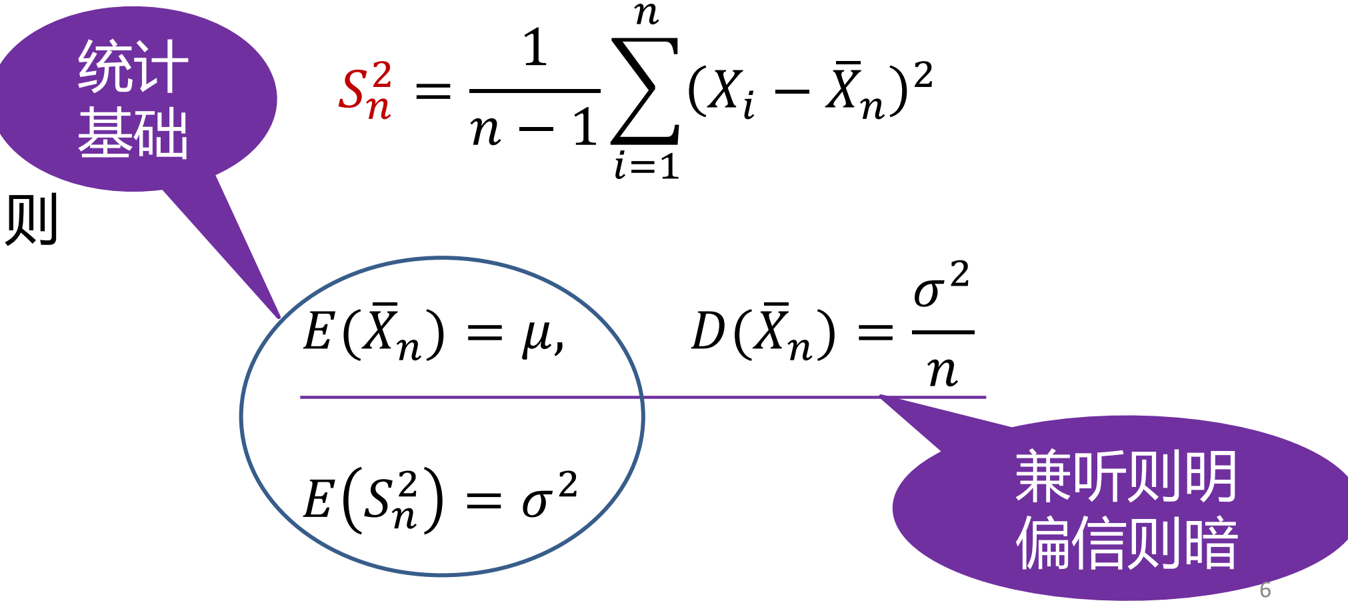
\includegraphics[width=0.5\textwidth]{figures/fig_statistics_basics.png}
    \caption{统计基础示意图（样本均值、样本方差的性质）}
    \label{fig:statistics_basics}
\end{figure}

\subsubsection{切比雪夫不等式}

\begin{theorem}[切比雪夫(Chebyshev)不等式]
设随机变量$X$具有数学期望$E(X)=\mu$，方差$D(X)=\sigma^{2}$，则对于任意正数$\varepsilon$，不等式
\[
P\{|X-\mu|\geq\varepsilon\}\leq\frac{\sigma^{2}}{\varepsilon^{2}}
\]
成立，等价地
\[
P\{|X-\mu|<\varepsilon\}\geq 1-\frac{\sigma^{2}}{\varepsilon^{2}}.
\]
\end{theorem}

\begin{figure}[htbp]
    \centering
    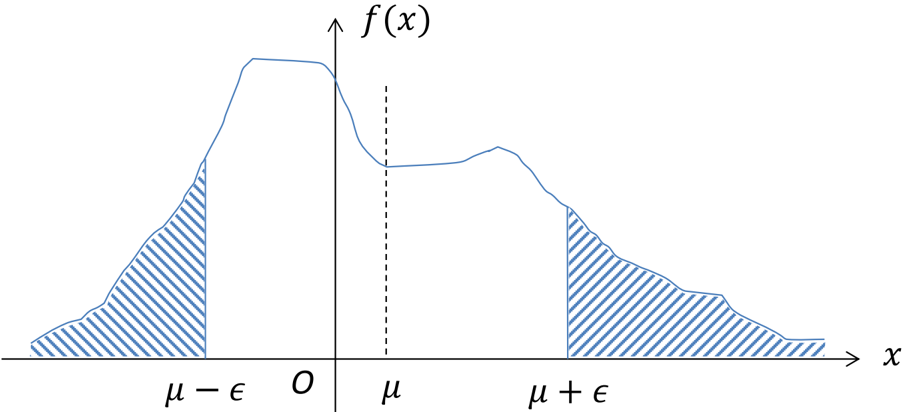
\includegraphics[width=0.5\textwidth]{figures/fig_chebyshev.png}
    \caption{切比雪夫不等式示意图（概率密度曲线，两侧尾部阴影区域）}
    \label{fig:chebyshev}
\end{figure}

\textbf{证明}：
\[
P\{|X-\mu|\geq\varepsilon\}=\int_{|x-\mu|\geq\varepsilon}f(x)\,dx
\leq\int_{|x-\mu|\geq\varepsilon}\frac{(x-\mu)^{2}}{\varepsilon^{2}}f(x)\,dx
\leq\frac{1}{\varepsilon^{2}}\int_{-\infty}^{+\infty}(x-\mu)^{2}f(x)\,dx
=\frac{\sigma^{2}}{\varepsilon^{2}}.
\]

由切比雪夫不等式可证明下面的性质：

\begin{property}
$D(X)=0\Leftrightarrow P\{X=E(X)\}=1$。
\end{property}

\textbf{证明}：由方差定义，若$X=\text{Const}$，则显然$D(X)=0$。

若$D(X)=0$，假设$P\{X=E(X)\}<1$，即存在$\varepsilon>0$，使得$P\{|X-E(X)|\geq\varepsilon\}>0$，但由切比雪夫不等式
\[
P\{|X-E(X)|\geq\varepsilon\}\leq\frac{D(X)}{\varepsilon^{2}}=0,
\]
与假设矛盾，于是$P\{X=E(X)\}=1$。

\section{协方差及相关系数}

对于二维随机变量$(X,Y)$，除了需要讨论$X$与$Y$的数学期望和方差外，还需讨论$X$与$Y$之间相互关系的数字特征。

\subsection{协方差与相关系数的定义}

\begin{definition}[协方差]
量$E\{[X-E(X)][Y-E(Y)]\}$称为随机变量$X$与$Y$的\textbf{协方差}，记为$\mathrm{Cov}(X,Y)$，即
\[
\mathrm{Cov}(X,Y)=E\{[X-E(X)][Y-E(Y)]\}.
\]
称
\[
\rho_{XY}=\frac{\mathrm{Cov}(X,Y)}{\sqrt{D(X)}\sqrt{D(Y)}}
\]
为随机变量$X$与$Y$的\textbf{相关系数}。$\rho_{XY}$无量纲，有时又称为\textbf{标准协方差}。
\end{definition}

\subsection{协方差的性质}

\begin{property}[协方差的基本性质]
\begin{enumerate}[label=\arabic*.,leftmargin=2em]
    \item 对称性：$\mathrm{Cov}(X,Y)=\mathrm{Cov}(Y,X)$。
    \item $\mathrm{Cov}(X,Y)=E(XY)-E(X)E(Y)$。
    
    \textbf{证明}：
    \begin{align*}
    \mathrm{Cov}(X,Y)&=E\{[X-E(X)][Y-E(Y)]\}\\
    &=E[XY-YE(X)-XE(Y)+E(X)E(Y)]\\
    &=E(XY)-2E(X)E(Y)+E(X)E(Y)\\
    &=E(XY)-E(X)E(Y).
    \end{align*}
    
    \item $\mathrm{Cov}(aX,bY)=ab\,\mathrm{Cov}(X,Y)$，其中$a,b$为常数。
    \item $\mathrm{Cov}(X_{1}+X_{2},Y)=\mathrm{Cov}(X_{1},Y)+\mathrm{Cov}(X_{2},Y)$。
    \item 若$X=Y$，则退化为$\mathrm{Cov}(X,X)=D(X)$。
    \item $\mathrm{Cov}(aX,bX)=ab\,D(X)$。
\end{enumerate}
\end{property}

\subsection{随机变量和的方差}

由协方差定义，有
\[
D(X+Y)=E\{[(X+Y)-E(X+Y)]^{2}\}=D(X)+D(Y)+2\mathrm{Cov}(X,Y).
\]
若$X$与$Y$相互独立，则有$\mathrm{Cov}(X,Y)=E(XY)-E(X)E(Y)=0$，于是
\[
D(X+Y)=D(X)+D(Y).
\]

\begin{example}[二维正态分布的相关系数]
设$(X,Y)\sim N(\mu_{1},\mu_{2},\sigma_{1}^{2},\sigma_{2}^{2},\rho)$，求$X$与$Y$的相关系数。
\end{example}

\textbf{解}：二维正态分布的密度函数为
\[
f(x,y)=\frac{1}{2\pi\sigma_{1}\sigma_{2}\sqrt{1-\rho^{2}}}
\exp\left\{-\frac{1}{2(1-\rho^{2})}\left[\frac{(x-\mu_{1})^{2}}{\sigma_{1}^{2}}
-\frac{2\rho(x-\mu_{1})(y-\mu_{2})}{\sigma_{1}\sigma_{2}}
+\frac{(y-\mu_{2})^{2}}{\sigma_{2}^{2}}\right]\right\}.
\]
由前面第三章知边缘分布
\[
f_{X}(x)=\frac{1}{\sqrt{2\pi}\sigma_{1}}e^{-\frac{(x-\mu_{1})^{2}}{2\sigma_{1}^{2}}},\qquad
f_{Y}(y)=\frac{1}{\sqrt{2\pi}\sigma_{2}}e^{-\frac{(y-\mu_{2})^{2}}{2\sigma_{2}^{2}}}.
\]
由本章第一、第二节有
\[
E(X)=\mu_{1},\quad E(Y)=\mu_{2},\quad D(X)=\sigma_{1}^{2},\quad D(Y)=\sigma_{2}^{2}.
\]
由协方差定义，作变量代换
\[
t=\frac{1}{\sqrt{1-\rho^{2}}}\left(\frac{y-\mu_{2}}{\sigma_{2}}-\rho\frac{x-\mu_{1}}{\sigma_{1}}\right),\qquad
u=\frac{x-\mu_{1}}{\sigma_{1}},
\]
计算可得
\[
\mathrm{Cov}(X,Y)=\rho\sigma_{1}\sigma_{2}.
\]
于是
\[
\rho_{XY}=\frac{\mathrm{Cov}(X,Y)}{\sigma_{1}\sigma_{2}}=\rho.
\]

\begin{note}
\begin{enumerate}[leftmargin=2em]
    \item 二维正态分布密度函数中，参数$\rho$代表了$X$与$Y$的相关系数；
    \item 对二维正态分布而言，相关系数为零等价于$X$与$Y$相互独立。
\end{enumerate}
\end{note}

\begin{example}[线性组合的期望与方差]
已知随机变量$X,Y$分别服从$N(1,3^{2})$，$N(0,4^{2})$，且$\rho_{XY}=-1/2$。设$Z=\dfrac{X}{3}+\dfrac{Y}{2}$，求：
\begin{enumerate}[label=(\arabic*),leftmargin=2em]
    \item $Z$的数学期望和方差；
    \item $X$与$Z$的相关系数；
    \item $X$与$Z$是否独立？为何？
\end{enumerate}
\end{example}

\textbf{解}：(1)
\[
E(Z)=\frac{1}{3}E(X)+\frac{1}{2}E(Y)=\frac{1}{3}.
\]
\begin{align*}
D(Z)&=D\left(\frac{X}{3}\right)+D\left(\frac{Y}{2}\right)+2\mathrm{Cov}\left(\frac{X}{3},\frac{Y}{2}\right)\\
&=\frac{1}{9}D(X)+\frac{1}{4}D(Y)+\frac{1}{3}\mathrm{Cov}(X,Y)\\
&=1+4+\frac{1}{3}\rho_{XY}\sqrt{D(X)}\sqrt{D(Y)}\\
&=5+\frac{1}{3}\left(-\frac{1}{2}\right)\times 3\times 4=3.
\end{align*}

(2)
\begin{align*}
\mathrm{Cov}(X,Z)&=\mathrm{Cov}\left(X,\frac{X}{3}+\frac{Y}{2}\right)\\
&=\frac{1}{3}\mathrm{Cov}(X,X)+\frac{1}{2}\mathrm{Cov}(X,Y)\\
&=\frac{1}{3}D(X)+\frac{1}{2}\rho_{XY}\sqrt{D(X)}\sqrt{D(Y)}\\
&=3-3=0.
\end{align*}
于是
\[
\rho_{XZ}=\frac{\mathrm{Cov}(X,Z)}{\sqrt{D(X)}\sqrt{D(Z)}}=0.
\]

(3) 注意到$X$和$Z$均为正态分布，且$\rho_{XZ}=0$，于是$X$与$Z$是相互独立的。

\subsection{方差、协方差与相关系数的实例}

\begin{figure}[htbp]
    \centering
    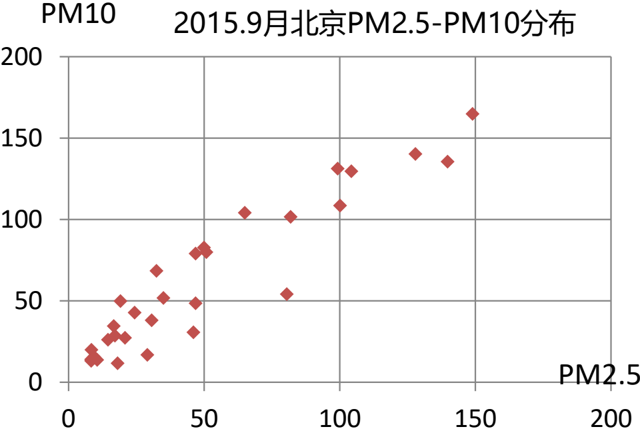
\includegraphics[width=0.6\textwidth]{figures/fig_pm25_pm10_scatter.png}
    \caption{2015年9月北京PM2.5-PM10分布散点图}
    \label{fig:pm25_pm10_scatter}
\end{figure}

\begin{figure}[htbp]
    \centering
    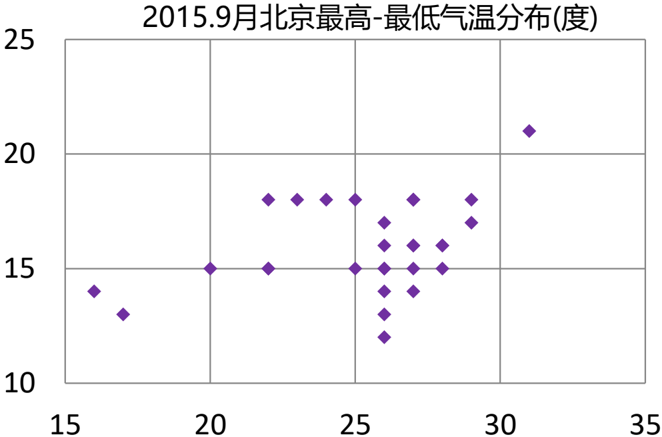
\includegraphics[width=0.6\textwidth]{figures/fig_temp_scatter.png}
    \caption{2015年9月北京最高-最低气温分布散点图}
    \label{fig:temp_scatter}
\end{figure}

\begin{figure}[htbp]
    \centering
    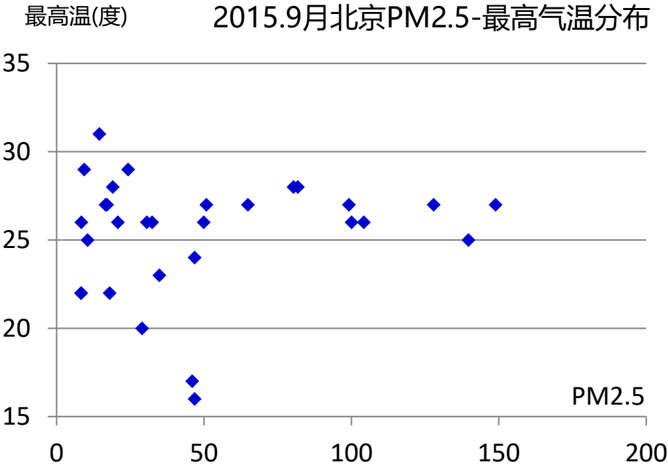
\includegraphics[width=0.6\textwidth]{figures/fig_pm25_high_temp.png}
    \caption{2015年9月北京PM2.5-最高气温分布散点图}
    \label{fig:pm25_high_temp}
\end{figure}

\begin{figure}[htbp]
    \centering
    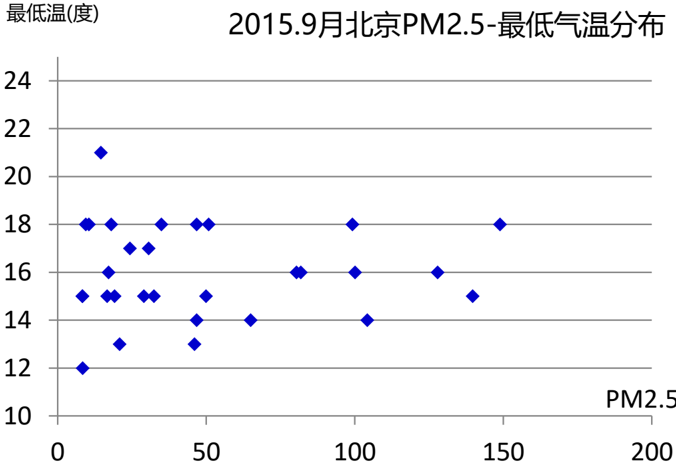
\includegraphics[width=0.6\textwidth]{figures/fig_pm25_low_temp.png}
    \caption{2015年9月北京PM2.5-最低气温分布散点图}
    \label{fig:pm25_low_temp}
\end{figure}

PM2.5/PM数据源于：http://www.aqistudy.cn

气温数据源于：http://lishi.tianqi.com/

\subsection{相关系数的几何意义}

随机变量$X$与$Y$是否可以通过线性拟合（回归）加以逼近，考虑最小化均方误差
\[
\min_{a,b}\Bigl\{e=E\bigl[(Y-(a+bX))^{2}\bigr]\Bigr\}.
\]

\begin{figure}[htbp]
    \centering
    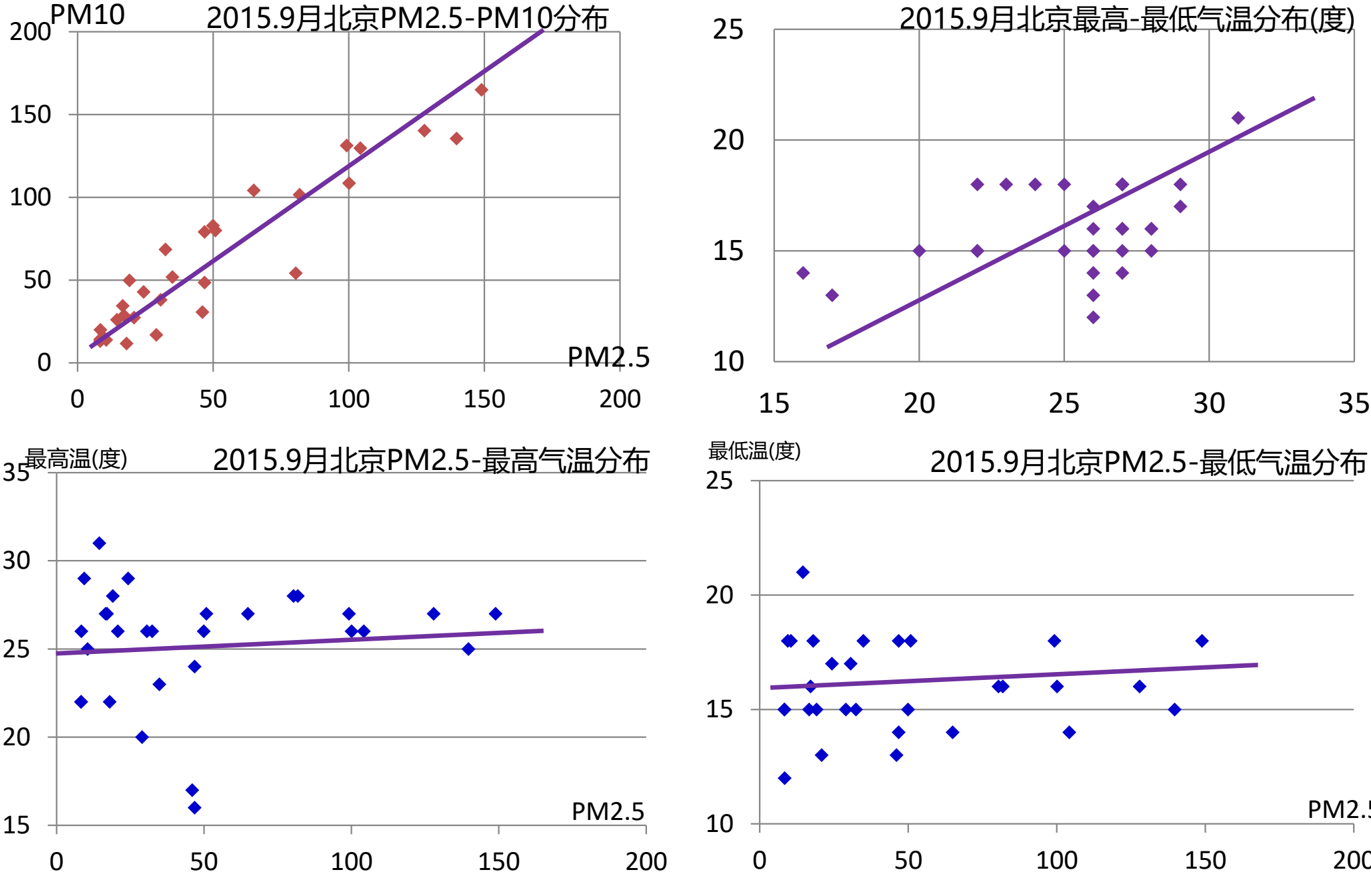
\includegraphics[width=0.6\textwidth]{figures/fig_linear_regression.png}
    \caption{PM2.5-PM10分布带线性回归线}
    \label{fig:linear_regression}
\end{figure}

求关于$a,b$的偏导，并令它们为零，有
\[
\begin{cases}
\dfrac{\partial e}{\partial a}=2a+2bE(X)-2E(Y)=0,\\[0.5em]
\dfrac{\partial e}{\partial b}=2bE(X^{2})-2E(XY)+2aE(X)=0.
\end{cases}
\]

解得
\[
a=E(Y)-\frac{E(X)\mathrm{Cov}(X,Y)}{D(X)},\qquad b=\frac{\mathrm{Cov}(X,Y)}{D(X)}.
\]

代回$e$的表达式：
\begin{align*}
e&=E\left[\left(Y-E(Y)-\frac{\mathrm{Cov}(X,Y)}{D(X)}(X-E(X))\right)^{2}\right]\\
&=D(Y)-\frac{[\mathrm{Cov}(X,Y)]^{2}}{D(X)}\\
&=D(Y)(1-\rho_{XY}^{2}).
\end{align*}

\textbf{几何解释}：
\begin{enumerate}[label=\arabic*.,leftmargin=2em]
    \item 当$|\rho_{XY}|$较大时，$e$较小，$X,Y$的线性关系较为紧密；$|\rho_{XY}|=1$时，$e=0$，$X$与$Y$以概率$1$线性相关。
    \item 当$|\rho_{XY}|$较小时，$e$较大，$X,Y$的线性关系较差；$\rho_{XY}=0$时，$X$与$Y$完全不相关。
\end{enumerate}

\subsection{随机变量的不相关与独立}

\begin{definition}[不相关]
若$\rho_{XY}=0$，则称随机变量$X$与$Y$\textbf{不相关}。
\end{definition}

\begin{note}
是否相关只是针对线性关系而言的，$X$与$Y$相互独立则是相对一般关系而言的。
\end{note}

随机变量$X$与$Y$不相关（即$\rho_{XY}=0$）的等价条件：
\begin{enumerate}[label=(\arabic*),leftmargin=2em]
    \item $\mathrm{Cov}(X,Y)=0$；
    \item $E(XY)-E(X)E(Y)=0$，即$E(XY)=E(X)E(Y)$；
    \item $D(X+Y)=D(X)+D(Y)$。
\end{enumerate}

\begin{property}
$X$与$Y$相互独立$\Longrightarrow$$X$与$Y$一定不相关，反之则不然。
\end{property}

\begin{example}[不相关但不独立]
设$\theta$服从$[0,2\pi]$上的均匀分布，$\xi=\cos\theta$，$\eta=\cos(\theta+a)$，这里$a$是常数，求$\xi$和$\eta$的相关系数。
\end{example}

\textbf{解}：
\[
E(\xi)=\frac{1}{2\pi}\int_{0}^{2\pi}\cos x\,dx=0,\qquad
E(\eta)=\frac{1}{2\pi}\int_{0}^{2\pi}\cos(x+a)\,dx=0.
\]
\[
D(\xi)=\frac{1}{2\pi}\int_{0}^{2\pi}\cos^{2}x\,dx=\frac{1}{2},\qquad
D(\eta)=\frac{1}{2\pi}\int_{0}^{2\pi}\cos^{2}(x+a)\,dx=\frac{1}{2}.
\]
\[
\mathrm{Cov}(\xi,\eta)=\frac{1}{2\pi}\int_{0}^{2\pi}\cos x\cos(x+a)\,dx=\frac{1}{2}\cos a.
\]
于是相关系数
\[
\rho=\frac{\mathrm{Cov}(\xi,\eta)}{\sqrt{D(\xi)}\sqrt{D(\eta)}}=\cos a.
\]

\begin{enumerate}[label=\arabic*.,leftmargin=2em]
    \item $a=0$时，$\rho=1$，$\xi=\eta$，存在线性关系；
    \item $a=\pi$时，$\rho=-1$，$\xi=-\eta$，存在线性关系；
    \item $a=\dfrac{\pi}{2}$或$a=\dfrac{3\pi}{2}$时，$\rho=0$，$\xi$与$\eta$不相关，但$\xi^{2}+\eta^{2}=1$，因此$\xi$与$\eta$不独立。
\end{enumerate}

\section{矩、协方差矩阵}

\subsection{矩的定义}

\begin{definition}[矩]
设$X$和$Y$是随机变量，
\begin{enumerate}[label=\arabic*.,leftmargin=2em]
    \item 若$E(X^{k})\;(k=1,2,\ldots)$存在，则称它为$X$的\textbf{$k$阶原点矩}，简称\textbf{$k$阶矩}。
    \item 若$E\{[X-E(X)]^{k}\}\;(k=2,3,\ldots)$存在，则称它为$X$的\textbf{$k$阶中心矩}。
    \item 若$E(X^{k}Y^{l})\;(k,l=1,2,\ldots)$存在，则称它为$X$和$Y$的\textbf{$k+l$阶混合矩}。
    \item 若$E\{[X-E(X)]^{k}[Y-E(Y)]^{l}\}\;(k,l=1,2,\ldots)$存在，则称它为$X$和$Y$的\textbf{$k+l$阶混合中心矩}。
\end{enumerate}
\end{definition}

\begin{note}
\begin{itemize}[leftmargin=2em]
    \item 数学期望$E(X)$是$X$的一阶原点矩；
    \item 方差$D(X)$是$X$的二阶中心矩；
    \item 协方差$\mathrm{Cov}(X,Y)$是$X$与$Y$的二阶混合中心矩；
    \item 三阶中心矩可以用来衡量随机变量的分布是否有偏；
    \item 更高阶中心矩可以用来衡量随机变量的分布在均值附近的陡峭程度如何。
\end{itemize}
高阶矩很少使用。
\end{note}

\begin{figure}[htbp]
    \centering
    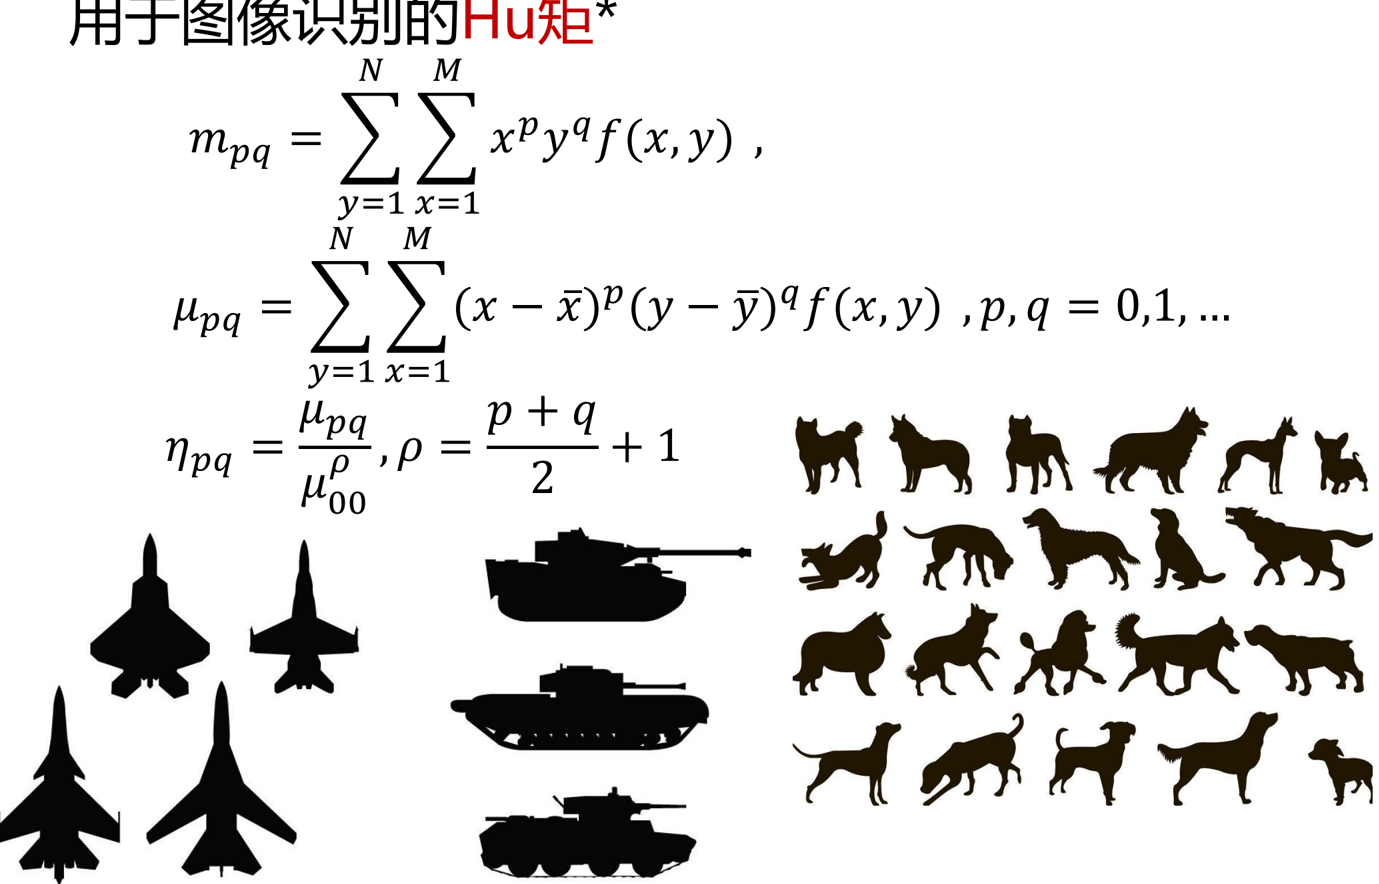
\includegraphics[width=0.5\textwidth]{figures/fig_hu_moments.png}
    \caption{Hu矩用于图像识别的示意图}
    \label{fig:hu_moments}
\end{figure}

\subsection{协方差矩阵}

\begin{definition}[协方差矩阵]
设$n$维随机变量$(X_{1},X_{2},\ldots,X_{n})$的二阶混合中心矩
\[
c_{ij}=\mathrm{Cov}(X_{i},X_{j})=E\{[X_{i}-E(X_{i})][X_{j}-E(X_{j})]\},\quad i,j=1,2,\ldots,n
\]
都存在，则称矩阵
\[
\boldsymbol{C}=\left[\begin{matrix}
c_{11} & c_{12} & \cdots & c_{1n}\\
c_{21} & c_{22} & \cdots & c_{2n}\\
\vdots & \vdots & \ddots & \vdots\\
c_{n1} & c_{n2} & \cdots & c_{nn}
\end{matrix}\right]
\]
为$n$维随机变量的\textbf{协方差矩阵}。
\end{definition}

\begin{note}
\begin{enumerate}[leftmargin=2em]
    \item 协方差矩阵是一个对称非负定矩阵；
    \item 协方差矩阵可用来表示多维随机变量的概率密度，从而可通过协方差矩阵达到对多维随机变量的研究。
\end{enumerate}
\end{note}

\subsection{二维正态分布的矩阵表示}

设$(X_{1},X_{2})\sim N(\mu_{1},\mu_{2},\sigma_{1}^{2},\sigma_{2}^{2},\rho)$，引入
\[
\boldsymbol{x}=\left[\begin{matrix}x_{1}\\x_{2}\end{matrix}\right],\qquad
\boldsymbol{\mu}=\left[\begin{matrix}\mu_{1}\\\mu_{2}\end{matrix}\right],
\]
协方差矩阵为
\[
\boldsymbol{C}=\left[\begin{matrix}
c_{11} & c_{12}\\
c_{21} & c_{22}
\end{matrix}\right]
=
\left[\begin{matrix}
\sigma_{1}^{2} & \rho\sigma_{1}\sigma_{2}\\
\rho\sigma_{1}\sigma_{2} & \sigma_{2}^{2}
\end{matrix}\right].
\]
其逆矩阵为
\[
\boldsymbol{C}^{-1}=\frac{1}{\sigma_{1}^{2}\sigma_{2}^{2}(1-\rho^{2})}
\left[\begin{matrix}
\sigma_{2}^{2} & -\rho\sigma_{1}\sigma_{2}\\
-\rho\sigma_{1}\sigma_{2} & \sigma_{1}^{2}
\end{matrix}\right].
\]

注意到
\[
(\boldsymbol{x}-\boldsymbol{\mu})^{\mathrm{T}}\boldsymbol{C}^{-1}(\boldsymbol{x}-\boldsymbol{\mu})
=\frac{1}{1-\rho^{2}}\left[\frac{(x_{1}-\mu_{1})^{2}}{\sigma_{1}^{2}}
-2\rho\frac{(x_{1}-\mu_{1})(x_{2}-\mu_{2})}{\sigma_{1}\sigma_{2}}
+\frac{(x_{2}-\mu_{2})^{2}}{\sigma_{2}^{2}}\right].
\]
故
\[
f(x_{1},x_{2})=\frac{1}{2\pi(\det\boldsymbol{C})^{1/2}}
\exp\left[-\frac{1}{2}(\boldsymbol{x}-\boldsymbol{\mu})^{\mathrm{T}}\boldsymbol{C}^{-1}(\boldsymbol{x}-\boldsymbol{\mu})\right].
\]

\subsection{\texorpdfstring{$n$}{n}维正态分布}

类似地，可以推广到$n$维：
\[
\boldsymbol{x}=\left[\begin{matrix}x_{1}\\x_{2}\\\vdots\\x_{n}\end{matrix}\right],\qquad
\boldsymbol{\mu}=\left[\begin{matrix}\mu_{1}\\\mu_{2}\\\vdots\\\mu_{n}\end{matrix}\right],\qquad
\boldsymbol{C}=[c_{ij}]_{n\times n}.
\]
$(X_{1},X_{2},\ldots,X_{n})$的概率密度定义为
\[
f(x_{1},x_{2},\ldots,x_{n})=\frac{1}{(2\pi)^{n/2}|\boldsymbol{C}|^{1/2}}
\exp\left[-\frac{1}{2}(\boldsymbol{x}-\boldsymbol{\mu})^{\mathrm{T}}\boldsymbol{C}^{-1}(\boldsymbol{x}-\boldsymbol{\mu})\right].
\]

\subsection{\texorpdfstring{$n$}{n}维正态分布的性质}

\begin{property}[$n$维正态分布的性质]
\begin{enumerate}[label=\arabic*.,leftmargin=2em]
    \item $n$维正态变量$(X_{1},X_{2},\ldots,X_{n})$的每一个分量$X_{i}\;(i=1,2,\ldots)$都是正态变量；反之，若$X_{1},X_{2},\ldots,X_{n}$都是正态变量，且相互独立，则$(X_{1},X_{2},\ldots,X_{n})$是$n$维正态变量。
    \item $n$维正态变量$(X_{1},X_{2},\ldots,X_{n})$服从$n$维正态分布$\Longleftrightarrow$$X_{1},X_{2},\ldots,X_{n}$的任意线性组合服从正态分布。
    \item 若$(X_{1},X_{2},\ldots,X_{n})$服从$n$维正态分布，设$Y_{1},Y_{2},\ldots,Y_{k}$是$X_{j}$的线性函数，则$(Y_{1},Y_{2},\ldots,Y_{k})$也服从多维正态分布。
    \item 设$(X_{1},X_{2},\ldots,X_{n})$服从$n$维正态分布，则$X_{1},X_{2},\ldots,X_{n}$相互独立$\Longleftrightarrow$$X_{1},X_{2},\ldots,X_{n}$两两不相关。
\end{enumerate}
\end{property}

\subsection{多元正态分布的数字特征与几何意义}

从一元分布到多元分布：
\begin{itemize}[leftmargin=2em]
    \item 一元正态分布的一组样本：$\{x_{1},x_{2},\ldots,x_{N}\}$；
    \item 多元正态分布的一组样本：$\{\boldsymbol{x}_{1},\boldsymbol{x}_{2},\ldots,\boldsymbol{x}_{N}\}$，其中$\boldsymbol{x}_{i}=[x_{i1},x_{i2},\ldots,x_{id}]^{\mathrm{T}}$，$i=1,\ldots,N$。
\end{itemize}

用矩阵表示为
\[
\boldsymbol{X}=[\boldsymbol{x}_{1},\boldsymbol{x}_{2},\ldots,\boldsymbol{x}_{N}]
=
\left[\begin{matrix}
x_{11} & \cdots & x_{N1}\\
\vdots & \ddots & \vdots\\
x_{1d} & \cdots & x_{Nd}
\end{matrix}\right].
\]

密度函数：
\[
f(\boldsymbol{x};\boldsymbol{\mu},\boldsymbol{\Sigma})=\frac{1}{(2\pi)^{d/2}|\boldsymbol{\Sigma}|^{1/2}}
\exp\left[-\frac{1}{2}(\boldsymbol{x}-\boldsymbol{\mu})^{\mathrm{T}}\boldsymbol{\Sigma}^{-1}(\boldsymbol{x}-\boldsymbol{\mu})\right].
\]

\textbf{多元分布的参数}
\begin{itemize}[leftmargin=2em]
    \item 均值（$d$维向量）：
    \[
    \boldsymbol{\mu}=\left[\begin{matrix}\mu_{1}\\\vdots\\\mu_{d}\end{matrix}\right].
    \]
    \item 协方差矩阵（$d\times d$矩阵）：
    \[
    \boldsymbol{\Sigma}=\left[\begin{matrix}
    \sigma_{11} & \cdots & \sigma_{1d}\\
    \vdots & \ddots & \vdots\\
    \sigma_{d1} & \cdots & \sigma_{dd}
    \end{matrix}\right].
    \]
    其中$\sigma_{ii}$为第$i$个特征的方差，$\sigma_{ij}$为第$i,j$个特征的协方差。当$\boldsymbol{\Sigma}$为对角阵时，不同特征之间不具备相关性。
\end{itemize}

\textbf{均值与协方差对样本分布的影响}：

\begin{itemize}[leftmargin=2em]
    \item $\boldsymbol{\mu}_{1}=\left[\begin{matrix}0\\0\end{matrix}\right]$，$\boldsymbol{\Sigma}_{1}=\left[\begin{matrix}1&0\\0&1\end{matrix}\right]$：特征彼此不相关，形状正圆；
    \item $\boldsymbol{\mu}_{2}=\left[\begin{matrix}0\\-7\end{matrix}\right]$，$\boldsymbol{\Sigma}_{2}=\left[\begin{matrix}4&0\\0&0.25\end{matrix}\right]$：特征彼此不相关，第一维特征方差较大；
    \item $\boldsymbol{\mu}_{3}=\left[\begin{matrix}4\\4\end{matrix}\right]$，$\boldsymbol{\Sigma}_{3}=\left[\begin{matrix}4&-3\\-3&0.25\end{matrix}\right]$：两维特征之间负相关，左上方倾斜椭圆。
\end{itemize}

\begin{figure}[htbp]
    \centering
    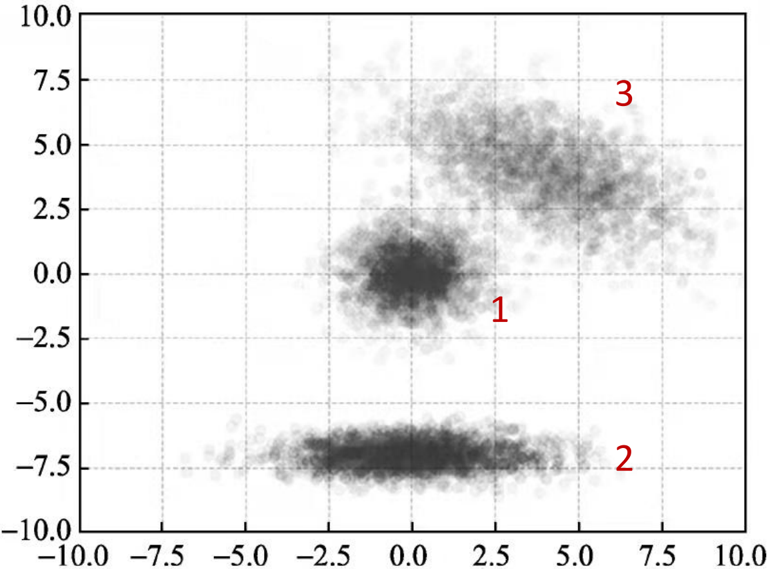
\includegraphics[width=0.6\textwidth]{figures/fig_multivariate_normal_scatter.png}
    \caption{不同均值和协方差矩阵对应的二维正态分布样本散点图（三组对比）}
    \label{fig:multivariate_normal_scatter}
\end{figure}

\textbf{多元正态分布的几何特征}：

协方差矩阵分解：$\boldsymbol{\Sigma}=\boldsymbol{Q}\boldsymbol{\Lambda}\boldsymbol{Q}^{\mathrm{T}}$，其中$\boldsymbol{Q}\boldsymbol{Q}^{\mathrm{T}}=\boldsymbol{I}$，
\[
\boldsymbol{\Lambda}=\left[\begin{matrix}
\lambda_{1} & & \\
& \ddots & \\
& & \lambda_{d}
\end{matrix}\right].
\]

协方差矩阵的逆：
\[
\boldsymbol{\Sigma}^{-1}=\boldsymbol{Q}\boldsymbol{\Lambda}^{-1}\boldsymbol{Q}^{\mathrm{T}}
=\sum_{i=1}^{d}\frac{1}{\lambda_{i}}\boldsymbol{q}_{i}\boldsymbol{q}_{i}^{\mathrm{T}}.
\]

概率密度表达：
\[
(\boldsymbol{x}-\boldsymbol{\mu})^{\mathrm{T}}\boldsymbol{\Sigma}^{-1}(\boldsymbol{x}-\boldsymbol{\mu})
=\sum_{i=1}^{d}\frac{1}{\lambda_{i}}(\boldsymbol{x}-\boldsymbol{\mu})^{\mathrm{T}}\boldsymbol{q}_{i}\boldsymbol{q}_{i}^{\mathrm{T}}(\boldsymbol{x}-\boldsymbol{\mu})
=\sum_{i=1}^{d}\frac{y_{i}^{2}}{\lambda_{i}},
\]
其中$y_{i}=(\boldsymbol{x}-\boldsymbol{\mu})^{\mathrm{T}}\boldsymbol{q}_{i}$。

当$d=2$时，
\[
\frac{y_{1}^{2}}{\lambda_{1}}+\frac{y_{2}^{2}}{\lambda_{2}}=1
\]
表示椭圆，$\boldsymbol{q}_{1}$和$\boldsymbol{q}_{2}$为其长轴和短轴方向，长度分别为$\sqrt{\lambda_{1}}$和$\sqrt{\lambda_{2}}$。$y_{1}$和$y_{2}$为样本在$\boldsymbol{q}_{1}$和$\boldsymbol{q}_{2}$上的投影长度。

当$\dfrac{y_{1}^{2}}{\lambda_{1}}+\dfrac{y_{2}^{2}}{\lambda_{2}}=\text{常数}$，每个椭圆上样本出现的概率相同；越大的椭圆上分布的样本概率越小。

\begin{figure}[htbp]
    \centering
    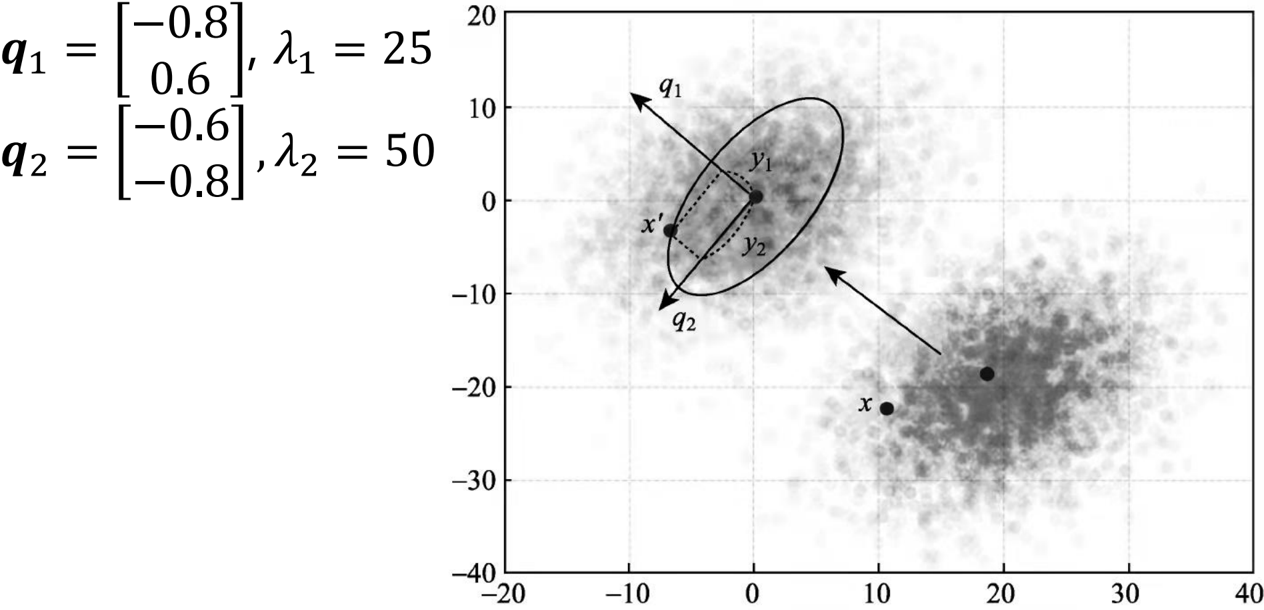
\includegraphics[width=0.6\textwidth]{figures/fig_covariance_eigen_decomposition.png}
    \caption{协方差矩阵特征分解几何示意图（椭圆、长轴短轴、样本点投影）}
    \label{fig:covariance_eigen_decomposition}
\end{figure}

\begin{example}[协方差矩阵特征分解]
设
\[
\boldsymbol{\mu}=\left[\begin{matrix}20\\-20\end{matrix}\right],\qquad
\boldsymbol{\Sigma}=\left[\begin{matrix}34&12\\12&41\end{matrix}\right].
\]
则
\[
\boldsymbol{q}_{1}=\left[\begin{matrix}-0.8\\0.6\end{matrix}\right],\;\lambda_{1}=25,\qquad
\boldsymbol{q}_{2}=\left[\begin{matrix}-0.6\\-0.8\end{matrix}\right],\;\lambda_{2}=50.
\]
\end{example}

% 图：上述均值和协方差对应的二维正态分布样本及特征向量示意图

\subsection{利用协方差进行识别}

一种局部描述子，在纹理分类、物体检测等方面获得很好的应用。用$d$维特征（比如R,G,B和前$2$阶差分）的协方差描述了感兴趣的区域。协方差矩阵不在欧氏空间上，因此采用广义特征值表示的距离度量。

（Tuzel, Porikli, and Peter Meer, Region Covariance: A Fast Descriptor for Detection and Classification, ECCV 2006）

\textbf{作为区域描述子}

给定区域$R$，其尺寸为$W\times H$。$\{\boldsymbol{z}_{k}\}_{k=1,2,\ldots,n}\in R$为$R$中的$n$个$d$维特征，采用$d\times d$协方差矩阵作为特征描述：
\[
\boldsymbol{C}_{R}=\frac{1}{n-1}\sum_{k=1}^{n}(\boldsymbol{z}_{k}-\boldsymbol{\mu})(\boldsymbol{z}_{k}-\boldsymbol{\mu})^{\mathrm{T}},
\]
其中$\boldsymbol{\mu}$是特征点的均值向量。

\textbf{方法特点}
\begin{itemize}[leftmargin=2em]
    \item \textbf{自然的特征融合方式}：对角线对应每个特征的方差，非对角线对应特征间的相关性；
    \item \textbf{噪声可以用平均的方法滤除}；
    \item \textbf{特征维度低}：直方图特征维度为$\prod_{i=1}^{d}h_{i}$（$h_{i}$为特征$i$的Bin数量），原始数据维数为$n\times d$，协方差特征维数为$(d^{2}+d)/2$；
    \item \textbf{一定尺度上的旋转和尺度不变}。
\end{itemize}

\textbf{距离计算}

协方差矩阵的距离不能用欧氏空间计算。两个协方差矩阵的不相似度定义为
\[
\rho(\boldsymbol{C}_{1},\boldsymbol{C}_{2})=\sqrt{\sum_{i=1}^{n}\ln^{2}\lambda_{i}(\boldsymbol{C}_{1},\boldsymbol{C}_{2})},
\]
其中$\lambda_{i}(\boldsymbol{C}_{1},\boldsymbol{C}_{2})$是$\boldsymbol{C}_{1},\boldsymbol{C}_{2}$的广义特征值，由下式计算获得：
\[
\lambda_{i}\boldsymbol{C}_{1}\boldsymbol{x}_{i}-\boldsymbol{C}_{2}\boldsymbol{x}_{i}=0,
\]
$\boldsymbol{x}_{i}$为第$i$个广义特征向量。

$\rho(\boldsymbol{C}_{1},\boldsymbol{C}_{2})$满足距离的非负性、交换性和三角不等式：
\begin{itemize}[leftmargin=2em]
    \item $\rho(\boldsymbol{C}_{1},\boldsymbol{C}_{2})\geq 0$，且$\rho(\boldsymbol{C}_{1},\boldsymbol{C}_{2})=0$当且仅当$\boldsymbol{C}_{1}=\boldsymbol{C}_{2}$；
    \item $\rho(\boldsymbol{C}_{1},\boldsymbol{C}_{2})=\rho(\boldsymbol{C}_{2},\boldsymbol{C}_{1})$；
    \item $\rho(\boldsymbol{C}_{1},\boldsymbol{C}_{2})+\rho(\boldsymbol{C}_{2},\boldsymbol{C}_{3})\geq\rho(\boldsymbol{C}_{1},\boldsymbol{C}_{3})$。
\end{itemize}

（W. Forstner, B. Moonen. A metric for covariance matrices. Technical report, Dept. of Geodesy and Geoinformatics, Stuttgart University, 1999）

\textbf{目标检测示例}

% 图：目标检测示例图（输入图像、协方差特征检测结果、直方图特征检测结果对比）
% 包括人脸检测、物体检测、场景识别等

\section{本章小结}

\begin{itemize}[leftmargin=2em]
    \item 总体特性是关心概率的目的；
    \item 从矩的角度理解多种数字特征；
    \item 矩包含了多种数字特征；
    \item 协方差矩阵包含了丰富的信息；
    \item 切比雪夫不等式；
    \item 不相关性与独立性之间的关系；
    \item 正态随机变量的特征。
\end{itemize}

\section*{作业}

\addcontentsline{toc}{section}{作业}

教材《概率论与数理统计》第四章（pp.~117--118）：\#34，\#35，\#37。

\end{document}